% Created 2024-04-19 Fri 02:49
% Intended LaTeX compiler: xelatex
\documentclass[11pt]{article}
\usepackage{graphicx}
\usepackage{longtable}
\usepackage{wrapfig}
\usepackage{rotating}
\usepackage[normalem]{ulem}
\usepackage{amsmath}
\usepackage{amssymb}
\usepackage{capt-of}
\usepackage{hyperref}
\author{saltb0rn}
\date{2018-08-31}
\title{Emacs Tips(持续更新)}
\hypersetup{
 pdfauthor={saltb0rn},
 pdftitle={Emacs Tips(持续更新)},
 pdfkeywords={},
 pdfsubject={},
 pdfcreator={Emacs 29.3 (Org mode 9.6.15)}, 
 pdflang={English}}
\begin{document}

\maketitle
\tableofcontents

\index{Emacs Tips(持续更新)}
\begin{abstract}
如果学一样东西不做知识管理的话,时间久了就会陷入Problem-Google-Solution-Forgotten 这样的循环中,记得读书时候有人说,看那个人做笔记那么

认真但还是考不好,真蠢.首先我个人不认为做笔记是一件蠢事,不过做笔记是需要技巧的,那个考不好的人可能是这里出了问题,或者只是他单纯的只是做笔

记而已.每当遇到问题去Google实际是一件很浪费时间的事情,为何不把内存里面的数据持久化下并且给它这个索引呢?记录的东西大部份都是很琐碎的,毕竟

是因为琐碎才要以这种形似记录下来.

P.S: 这文章做为我个人的知识管理方案之一会一直会更新.为什么不把每个话题分开写,那时因为记录的东西太琐碎了,不记录又不好,所以才写成一篇,不过分量大的话题会分开写,比如一些packages的用法.
\end{abstract}

\section{使用Emacs的一些tips}
\label{sec:org746168d}

\begin{itemize}
\item 如何快速了解Emacs内置库和内置功能的用法

很多人,包括我,都很好奇写Emacs Lisp的高人是如何知道那么多奇怪的功能,而且这些功能文档上又没提到.

现在有答案了,以下提示可以帮助你快速浏览这些奇怪的功能.

\begin{enumerate}
\item \texttt{C-h p},根据分类浏览,缺点里面会混杂一些非内置的库并且貌似不全

\item \texttt{M-x find-library},根据名字搜索库,缺点没有一个系统的分类

\item \texttt{M-x apropos-library},根据名字搜索库,可以看到库里面全部重要的定义

\item \texttt{M-x find-function} 查看函数定义, \texttt{C-h f} 或 \texttt{M-x describe-function} 查看函数描述以及用法

\item \texttt{M-x find-variable} 查看变量定义, \texttt{C-h v} 或 \texttt{M-x describe-variable} 查看变量描述以及用法

\item \texttt{C-h b} 或 \texttt{M-x describe-bindings} 查看所有按键绑定信息,包含了全局按键绑定,以及使用该命令当前的缓冲区所启用的 \texttt{minor mode} 和 \texttt{major mode} 的按键绑定.

可以配合 \texttt{apropos-library} 查看 \texttt{mode} 定义来快速掌握 \texttt{mode} 的使用.

\texttt{C-h k} 则查询某个绑定按键所对应的信息,比如绑定的是哪个命令,定义在哪里等等.

\item \texttt{C-h a} 或 \texttt{M-x apropos-command} 输入想要搜索的命令名字,模糊搜索命令,比 \texttt{M-x} 自动提示的好

\item \texttt{M-x apropos-variable} 输入需要搜索的变量名字,模糊搜索变量
\end{enumerate}

总之, \texttt{C-h} 是 \texttt{Emacs} 的 \texttt{help-command},可以通过它查看一些你不知道的Emacs的用法,是一个极其有用的内置文档,对于新手来说是一个不错的起点.比如 \texttt{C-h C-h} 就是一个非常有用的命令.

还有 \texttt{apropos} 库是一个辅助开发人员和用户的好东西,推荐使用.

上面都是一些比较常用和有用的命令,可以了解一下.

P.S: 顺便提一下,代码也是很重要的文档.

\item 如何学习库的API或者某一个API的用法呢

学习一个新的库/API也不是一件简单的事情,比如Emacs的文档上有很多东西都没给出,给出了但working examples太少,等等.对于这些问题我有一套学习策略.

\begin{enumerate}
\item 阅读库/API的文本文档/维基

文档虽然不一定有想要的答案,但依然是一个不错的起点.但是使用文档也是有学问的(,我没多少就是了).

\begin{enumerate}
\item 学习这个库/API之前了解所需要的概念和相关背景.

\textbf{比如},

\begin{itemize}
\item 这个库/API是解决什么问题的?

\item 它的使用流程是怎么样?(库的设计/架构)

\item 需要注意版本问题吗?(版本是否导致跟其它库/API冲突)

\item 它的changelog在哪?(一般文档里面有)

\item 需要了解的术语有哪些?(一般可以找文档里面找到,遇到不懂的就弄明白)
\end{itemize}

这样自己大概就可以给库的APIs分个类,对库有个全貌的认识,并且能够保证自己不会对这个库/API产生什么误解,对以后使用同样类型的库也能快速上手.

\item 了解文档.文档也是有分类的,每种文档的侧重点都不太一样.以Racket为例子,有 \texttt{tutorial}, \texttt{guide} 和 \texttt{reference} 3类.

\begin{itemize}
\item \texttt{tutorial} 就是给新手一个快速上手的例子,这种例子很丰富,但往往会忽略很多关于Racket东西.

\item \texttt{guide} 比 \texttt{tutorial} 更具备针对性,会利用例子对某一个点进行比较深入地说明,展示这个东西这么用,例子丰富.这类是给那种刷过一遍 \texttt{tutorial} 的新手使用的.

\item \texttt{reference} 比 \texttt{guide} 更加详细,大部份这类文档都仅仅给出一大段的说明,不会给出例子教你怎么使用,或者例子简陋难以掌握用法,这种文档是给熟悉了Racket一段时间的开发人员查阅用的.(而Emacs的内置文档就是这样.)
\end{itemize}
\end{enumerate}

了解库的相关信息后,读懂文档应该就问题不大了.掌握了文档属性以后就可以知道该如何选择和使用文档了.

P.S: 身边有不少,包括我自己,这里怎么不对呢?跟文档说的不一样啊?这个库是不是有Bug啊?怎么这个库这么难用,就没有更好的解决方法吗?文档上面没有啊!.其实只要做足了功课,这些问题就很少听到了.不仅仅是读文档,读代码也是一样的.

\item 阅读别人利用该库/API写的代码

有时候文档上面过程关于某个API的例子很简陋或者没有给出例子,而自己又实在头疼,那么只能到网上找例子,比如Github的repo,gist,Stack Exchange,别人的blog,等等.

\item 阅读库/API的单元测试代码

如果找不到别人的代码可以去看一看这个库有没有单元测试的代码,如果有,那么它们就是你想要的API文档了.

\item 阅读库/API的源代码

如果单元测试的代码也没有,那么可以自己去读想要了解的API的源代码,使用到它的地方就是你想要的例子.

\item 请教别人

如果上面的方法全部失效,那去问别人吧.
\end{enumerate}

\item 快速做正则测试 (一次关于是否使用 \texttt{\textbackslash{}} 的思考,不仅仅限于 \texttt{Emacs Lisp})

首先要清楚一点, \texttt{Emacs Lisp} 严格上来说没有正则表达式这个数据类型, 它是直接用字符串来表示正则表达式.

这么说可能不太好理解, 就拿 \texttt{Python} 和 \texttt{JavaScript} 来说, 它们都有单独的语法来表示正则表达式.

\texttt{Python} 用 \texttt{r"."} 来表示匹配换行符号以为的任意一个字符的正则表达式, \texttt{JavaScript} 则使用 \texttt{/./} 来表示同样的正则表达式.

但 \texttt{Emacs Lisp} 它没有, 而是直接用"特殊"一点的字符串来表示: \texttt{"."}.

在表示文本的场合下它就是字符串, 在正则表达式场合下它就是正则表达式.

但是正则表达式是定义了一些有特殊含义的字符的, 比如句号(.), 它是用来表示换行符以外的任意一个字符的, 并非表示句号本身.

我们把表示字符本身叫做表达字符含义, 发挥正则定义叫做表达正则含义.

有一些特殊字符会同时存在两种含义, 这个时候就要求开发人员要对字符的含义进行选择.

具体做法就是使用 \texttt{\textbackslash{}} 字符放在需要进行选择的字符前面, 如果被标记的字符是有正则含义的特殊字符,

那它就会反向表达为字符含义, 否则就直接表达为正则含义.

就比如 \texttt{"\textbackslash{}."} 就是让句号表达了它的字符含义, 用来匹配句号本身.

\begin{quote}
实际上使用起来有两种情况, 在使用 \texttt{Emacs} 的交互命令时, 比如 \texttt{M-x re-search-forward},

假设想匹配当前缓冲区里的句号, 那么就得在 \texttt{minibuffer} 里面输入 \texttt{\textbackslash{}.}.

但是如果你是在写代码的时候进行对句号本身的匹配, 那么就得这么写:

\begin{verbatim}
(re-search-forward "\\.")
\end{verbatim}

你可以理解为 \texttt{minibuffer} 里面写的并不是编码中字符串(, 毕竟没有双引号包着), 而是人们眼中看到的字符串,

最终会在 \texttt{Emacs} 的内部处理中转化成编码中字符串.

怎么理解呢? 就比如说调用 \texttt{(insert "\textbackslash{}nabc")} 会在缓冲区中的光标位置插入一个换行和 \texttt{abc} 三个字符,

而不是看到 \texttt{\textbackslash{}nabc} 这一串东西.

使用这个例子是为了阐述一个道理: 实际编码和最终眼中看到的是不一样的. \texttt{minibuffer} 的正则表达式非常符合人们直觉上的正则表达式.

在编写 \texttt{Elisp} 的正则表达式时, 开发人员心里需要清楚编码字符串最终会转换称什么样的眼中字符串, 眼中字符串如果和心目中的正则表达式一致的话就是没写错.

转换的方法很简单: 忽略掉所有转义字符(escaped characters)及相关处理, 移除掉所有其它字符的一个前置 \texttt{\textbackslash{}} 符号.

所谓转义字符就是在字符串中有着由特殊含义的字符, 它们看起来像是一个字符串的字符, 比如前面提到的 \texttt{\textbackslash{}n}.

举些例子:

\begin{verbatim}
"abc\\.txt" => "abc\.txt"
"abc\\ndef" => "abc\ndef"
"abc\ndef" => "abc
def"
\end{verbatim}
\end{quote}

虽然说看上去对没有正则含义的字符使用 \texttt{\textbackslash{}} 标记好像什么问题, 但字符串本身也是有转义字符(escaped characters)的,

这种字符就是以 \texttt{\textbackslash{}} 开头的字符序列, 比如换行符 \texttt{\textbackslash{}n}, 因此开发人员不能乱用 \texttt{\textbackslash{}} 对字符进行标记.

此外, \texttt{Emacs Lisp} 的正则也像字符串那样定义了一些有着特殊含义的字符序列, 他们被称为特殊构造(special constructs).

比如 \texttt{\textbackslash{}(...\textbackslash{})}, 在正则表达式里面它是用来对匹配内容进行分组的, 要想发挥它们的正则作用, 字符串就得这么写: \texttt{"\textbackslash{}\textbackslash{}(...\textbackslash{}\textbackslash{})"};

再比如 \texttt{\textbackslash{}w} 是用来匹配单词组成(word-constituent)的字符, 需要这样 \texttt{"\textbackslash{}\textbackslash{}w"} 来发挥正则作用.

\begin{quote}
\begin{itemize}
\item 单词是由字母, 数字以及下划线组成, 这三种字符就叫做单词组成字符.

\item 特殊构造和特殊字符也是一样分两种使用情况.

在 \texttt{minibuffer} 进行输入的时候不需要多加一个 \texttt{\textbackslash{}}, 比如 \texttt{\textbackslash{}w} 就直接输入 \texttt{\textbackslash{}w};

在编码的时候就得写成 \texttt{"\textbackslash{}\textbackslash{}w"}.
\end{itemize}
\end{quote}

\texttt{Emacs} 提供了一些辅助编写正则表达式的工具, 本人还是极力推荐 \textbf{不要} 依赖这些工具.

跟 \texttt{Racket} 提供 \texttt{regexp-quote} 反输出用于匹配目标字符串的正则表达式一样, \texttt{Emacs} 也提供一些辅助工具帮助你写"RegEx":

对当前缓冲区即时比对正则表达式的 \texttt{M-x re-builder} (注意要写在它给你的双引号里面),以及简单强大的 \texttt{rx}.

早日熟悉 \texttt{Emacs} 的正则表达式可以让你最大化享受到文本处理的便利.

比如你想把缓冲区中 \texttt{adj(M)} 的 \texttt{adj()} 去掉留下 \texttt{M},

那么可以使用 \texttt{replace-regexp} 命令: \texttt{M-x replace-regexp RET adj(\textbackslash{}(.*\textbackslash{})) RET \textbackslash{}1},

这是无法只用一次 \texttt{replace-string} 命令来完成的.

\item Linux上远程编辑和编辑需要sudo认证的文件

使用tramp库,它不仅可以远程编辑文件,也可以sudo修改本地文件

\begin{enumerate}
\item 编辑远程文件

\texttt{C-x C-f} 输入 \texttt{/ssh:user@host\#port:/path/to/file}, 就是说通过 \texttt{ssh} 以 \texttt{user} 身份编辑 \texttt{host:port} 上的 \texttt{/path/to/file} 文件.

\item sudo修改文件

\texttt{C-x C-f} 输入 \texttt{/sudo::/path/to/file}, 这样打开 \texttt{/path/to/file} 的时候就会提示输入密码了
\end{enumerate}

\item \texttt{Emacs Lisp} 的交互式编程

和很多直译型语言一样, \texttt{Emacs Lisp} 也支持 \texttt{REPL},不过这个功能藏得挺深得, \texttt{M-x ielm}.

\texttt{ielm} 全称 \texttt{Inferior Emacs Lisp Mode}. \texttt{Inferior Modes} 是个好东西.

\item 如何了解在使用 \texttt{Emacs} 的过程中发生的事情

有时候想知道自己操作了什么,使用按键输入对应什么命令,使用命令时发生了什么事情.

这种时候就会想起日志,在网上搜索后发现有三种打印日志:

\textbf{使用 Emacs 自带的 \texttt{command-history} 变量,或者 (command-history)},

但是这种方式有很多信息没有记录下来,具体可以看 \texttt{(info "(elisp)Command Loop")};

\textbf{使用第三方库 command-log-mode},这种能记录大部分命令,比第一种方案好不少,支持日志序列化,

不过还是有些输入是没法记录下来的,比如 \texttt{Calc} 里的输入是没有被记录下来的;

\textbf{使用第三方库 interaction-log},相比 \texttt{command-log-mode} 支持实时日志打印,

并且能够记录下 \texttt{command-log-mode} 的一些盲点,比如上面提到在 \texttt{Calc} 的输入,还会记录下一些文件按加载信息,内容十分详细.

我个人是用的第三种方案.

\item 把提示输入yes或no简化成y或n

\begin{verbatim}
(fset 'yes-or-no-p 'y-or-n-p)
\end{verbatim}

\item \texttt{C-x C-e} 默认eval的输出太丑,怎么美化

\begin{verbatim}
(fset 'eval-last-sexp 'pp-eval-last-sexp)
\end{verbatim}

\item \texttt{Linux} 上无法在使用 \texttt{Fcitx} 输入中文?

这是 \texttt{Emacs} 的一个古老的 \href{https://wiki.archlinux.org/title/fcitx\#Emacs}{bug}, 解决方法就是修改 \texttt{LC\_CTYPE} 这个变量为 \texttt{zh\_CN.UTF-8} 再运行 \texttt{Emacs},

写脚本的时候需要这么写:

\begin{verbatim}
env LC_CTYPE=zh_CN.UTF-8 emacs
\end{verbatim}

如果只是在命令行里面运行, 可以偷懒点写成:

\begin{verbatim}
LC_CTYPE=zh_CN.UTF-8 emacs
\end{verbatim}

没有特殊情况就尽量用第一种形式.
\end{itemize}

\section{写 Elisp 时候遇到的一些问题}
\label{sec:orgf04bd4a}

\subsection{如何解决写Elisp时候遇到的一些需要密码认证的命令行操作}
\label{sec:orgdc565b6}

以在个人版的Debian上面安装nodejs为例子.

\begin{verbatim}
先了解一下sudo,sudo的作用就是以另外一个用户身份执行命令,默认身份是superuser(这里是root),执行时候需要提供这个用户的密码.
sudo有一个sudoers policy缓存凭证15分钟,除非重写了凭证,否则在这15分钟内以这个用户身份执行命令是不需要再次输入任何密码的.
\end{verbatim}

\begin{enumerate}
\item 利用tramp库,设定默认目录为"/sudo::"

\begin{verbatim}
(let ((default-directory "/sudo::"))
  (shell-command "apt-get install nodejs"))
\end{verbatim}

缺点就是认证后不会生成凭证

\item 对命令进行修改

\begin{verbatim}
(shell-command (string-join (list "echo" (shell-quote-argument (read-passwd "Password: "))
                                  "|" "sudo" "-S" "apt-get" "install" "nodejs") " "))
\end{verbatim}

缺点就是比较麻烦,也没凭证管理,优点就是你可以自己实现凭证管理(怎么安全管理是一个问题).

\item 使用 \texttt{eshell-command}

\begin{verbatim}
(eshell-command "sudo apt-get install nodejs")
\end{verbatim}

优点是简单,但还是没有凭证管理.
\end{enumerate}


\subsection{如何让调试器可以调试user-error?}
\label{sec:org53cb559}
\begin{verbatim}
写于 2018/10/21
\end{verbatim}

Drew已经在这\href{https://superuser.com/questions/782313/emacs-make-debug-on-error-catch-errors/782365}{里面}进行回答了,文档上只是做了暗示,之所以调试器不能调试 \texttt{user-error},那么是因为 \texttt{debug-ignored-errors} 这个变量有 \texttt{user-error} 这个变量,

\texttt{debug-ignored-errors} 是告诉 \texttt{Emacs Debugger} 忽略哪些错误,所以只需要把 \texttt{debug-ignored-errors} 里面的 \texttt{user-error} 条目清空掉就可以了.也就是说 \texttt{user-error} 实际上还是可以唤醒 \texttt{debugger}.

\begin{verbatim}
(setq debug-ignored-errors
      (remove-if
       (lambda (item) (eq item 'user-error))
       debug-ignored-errors))
\end{verbatim}


\subsection{Autoload函数引用未被require的变量,修改该变量后无法读取变量?}
\label{sec:org17d7844}
\begin{verbatim}
写于 2018/10/21
\end{verbatim}

注意: \textbf{该问题虽然已经解决了,但是途中遇到一个奇怪现象我没有办法解释,以后还是会更新}.

解决问题时候的 \texttt{org-mode} 版本为 \texttt{org-plus-contrib-20181015}.

实际情况就是: 写了一个函数 \texttt{publish-all-posts} 需要使用 \texttt{org-publish} 作为 \texttt{subroutine}, 主要是利用 \texttt{Emacs Lisp} 的动态作用域名来临时绑定全局变量,特别是 \texttt{org-publish-project-alist} 并且调用 \texttt{org-publish}.

目的是为了不污染全局变量和环境,然而有一个问题, \texttt{org-publish} 是 \texttt{Autoload} 函数,可是我并没有 \texttt{require} 它引用的变量 \texttt{org-publish-project-alist},就在我用 \texttt{let} 进行绑定的时候发生了一个奇怪现象.

第一次执行函数 \texttt{publish-all-posts} 的时候报错了: "Unknown component static in project DarkSalt",引发错误的函数是 \texttt{org-publish-expand-projects}, 这还是可以理解,因为 \texttt{org-publish-project-alist} 并没有进行全局绑定默认是 \texttt{nil} 所以引发异常.

我不能理解的地方就在于接下来函数 \texttt{publish-all-posts} 的调用居然正常,没有发生报错.我读了一下 \texttt{org-publish, org-publish-projects 和 org-publish-expand-projects} 这3个函数的源代码并没发现在哪里给 \texttt{org-publish-project-alist} 进行赋值.

不过我还是带着疑惑把\href{https://github.com/saltb0rn/emacs.d/commit/b146dffaa096683e1f1eee171d6e292af719cdb1\#diff-64ed6d0a7a4f2eaf33cacc2454a19cff}{报错解决}了, \texttt{require} \texttt{ox-publish} (也就是 \texttt{org-publish-project-alist} 的定义文件) 就可以解决问题,不过还是不明白这个奇怪现象的原因,有可能是我没有读透代码,所以这个问题不能算是完全解决.

\begin{verbatim}
(defun publish-all-posts (project &optional force async)
  "Now the project of blog is isolated from `org-publish-project-alist'.
That is, when calling `org-publish-project' or `org-publish' would not
see any project of blog, vice versa."
  (interactive
   (list (assoc (completing-read "Publish project: "
                                 blog-alist nil t)
                blog-alist)
         current-prefix-arg))
  (create-project-directory-if-necessary)
  (write-posts-to-tag-inc)
  (rewrite-theindex-inc)
  (let ((org-publish-project-alist blog-alist)
        (org-html-home/up-format (ht-get home/up-formats 'blog))
        (org-html-head (ht-get html-heads 'blog))
        (org-html-preamble nil)
        (org-html-doctype "html5")
        (org-html-link-home "/")
        (org-html-link-up "/")
        (org-export-with-toc nil)
        (org-export-with-author t)
        (org-export-with-email nil)
        (org-export-with-creator nil)
        (org-export-with-date nil)
        (org-export-with-section-numbers nil))
    (org-publish project))
  (rename-theindex-to-index))
\end{verbatim}


\subsection{如何请求接口(JSON)}
\label{sec:orgc374eb7}
\begin{verbatim}
写于 2019/2/26
\end{verbatim}
\texttt{Emacs Lisp} 没有 \texttt{Python} 那么直接的网络请求库,不过我们可以自己手动封装一下(这里只是提供一下思路)

\begin{verbatim}
(require 'json)
(require 'url)

(defstruct response headers body)

(defun url-open (url)
  "Return the response by requesting the url."
  (with-temp-buffer
    (insert-buffer (url-retrieve-synchronously url)) ;; the message containing the headers and body
    (set-buffer-multibyte t)
    (decode-coding-region (point-min) (point-max) 'utf-8) ;; needed if text contains non-ascii character
    (goto-char (point-min))
    (re-search-forward "^$" nil 'move)
    (make-response :headers (buffer-substring-no-properties (point-min) (point))
                   :body (buffer-substring-no-properties (point) (point-max)))))

(defun response-to-json (response)
  (json-read-from-string (response-body response)))

;; example
(response-to-json (url-open "https://api.jikan.moe/v3/anime/1/characters_staff"))
\end{verbatim}


\subsection{如果读取JSON文件}
\label{sec:org0814dfa}
\begin{verbatim}
写于 2020/10/26
\end{verbatim}
\texttt{Emacs Lisp} 读取 \texttt{JSON} 文件的方式比很多语言自带的灵活得多.

假设现有个JSON文件,

\begin{verbatim}
{
  "name": "xxxxx",
  "job": "xxxxxx",
  "projects": [
    {
      "name": "xxxxx",
      "date": "xxxxx",
      "about": "xxxxxxxxxx"
    },
    {
      "name": "xxxxx",
      "date": "xxxxx",
      "about": "xxxxxxxxxx"
    },
    {
      "name": "xxxxx",
      "date": "xxxxx",
      "about": "xxxxxxxxxx"
    }
  ]
}
\end{verbatim}

现在需要读取它的 "projects" 值并且重新封装成一个 \texttt{JSON},在 \texttt{Emacs Lisp} 里面可以这么做,

\begin{verbatim}
(require 'json)

(let* ((json-object-type 'alist)              ;; 指定 JSON 的对象解析为 alist 类型
       (json-array-type 'list)                ;; 指定 JSON 的数组解析为 list 类型
       (json-key-type 'keyword)               ;; 指定 JSON 的键解析为 keyword 类型
       (json (json-read-file "~/test.json")))
  (json-encode (alist-get :projects json)))
\end{verbatim}

如果你不喜欢把 \texttt{JSON} 的对象解析成 \texttt{alist}, 可以把 \texttt{json-object-type} 设置为 \texttt{hash-table}, \texttt{plist} 这样的值,

自由设置解析的类型正是 \texttt{Emacs Lisp} 的 \texttt{json.el} 的灵活之处.


\section{Emacs Lisp 学习笔记}
\label{sec:org59dbc11}

\begin{quote}
这段话写于 2018/9/30

\sout{最后更新于 2020/10/31}

最后更新于 2021/12/18

我会对这段内容进行改版,理由如下:

\begin{enumerate}
\item 距离刚开始写下这段内容已经过去快 3 年了,期间断断续续使用 \texttt{Emacs} 完成工作,查阅文档的能力已经挺熟练了,基本上每次看文档都不需要翻阅这里的内容

\item 查阅这里的内容只有两种情况: 某个 \texttt{API} 的文档描述没有提供例子以致难以理解其用法,以及某些概念不好理解.

这也是我最初写这段内容就是为了通过补充理解和例子来解决这两个问题,但写着写着,不知不觉就想把文档翻译一边了.

由于太罗嗦了,在我遇到问题时不能马上解决问题.每当这时候我都会想为啥当初要翻译文档,我要的是错题集,又不百科全书.

不过即便如此,这些内容里面还是有不少值得保留的东西.

\\[0pt]
\end{enumerate}

接下来我先要做的是对这段内容进行瘦身,然后针对于一些对于大部分人都不太好理解的概念,把我的理解整理下来,补充原本该有的例子.
\end{quote}

我是以终身使用 \texttt{Emacs} 的目的去学 \texttt{Emacs Lisp} 的,而提用 \texttt{Emacs Lisp} 的使用水平的最好方法就是掌握 \texttt{reference} 文档的使用.

加上网上对于 \texttt{Emacs} 的相关内容整体看下来相对较少,有些问题还搜索不到解决办法,这有两种可能,其他人没有遇到,问题无解,或者问题的描述不对,

这里的所有可能都只能靠自己去读 \texttt{reference} 找解决办法.

\texttt{Emacs Lisp} 的 \texttt{reference} 有一个特点,很多 \texttt{APIs} 的说明文档都缺乏详细的使用例子,

如果掌握了相关概念的话这都不是问题,可碰巧就是这方面做得不好,很多概念说明都不够直观,

明明只要画个简单的图就可以解决的问题,它就是没有这么做,不过这也只限于 \texttt{Emacs} 相关的 \texttt{APIs} 了.

\texttt{Emacs Lisp} 和其它语言一样有着这操作进程,线程的等等能力,也就是说,开发人员要像熟悉使用这部分的接口,就必须去了解这类的"通用概念",

这对于开发人员来是说百利而无一害的,遇到这类概念又不懂的话把就老实的补上吧.

我写这部分的笔记有两个目的: 一是为了直观理解 \texttt{Emacs} 那些不太容易理解的概念;二是为了针对通用概念进行补盲.

因此这部分笔记的信息量会比较大(我会在保证内容直观的前提下尽量精简),更新期也会很长,计划一个星期更新一个概念的笔记.

最后重伸一遍,这并不是 \texttt{APIs} 的笔记(我没有抄一遍 \texttt{reference} 的理由,顶多补充一些使用例子),而是一些概念的笔记.

当然不同版本的 \texttt{Emacs} 所关联的概念也会不一样,这些我会尽可能进行说明.

\subsection{Emacs Lisp 数据类型概览}
\label{sec:org0c26040}

\texttt{Emacs Lisp} 的数据类型分两大类: \textbf{语言内置的数据类型} 以及 \texttt{Emacs} 编辑器内置的数据类型.

所谓的语言内置的数据类型就是像整数,浮点数,字符串等等这些基本是编程语言都会有的类型;

像线程,进程这种类型是为了操作特定平台功能的数据类型而不属于语言内置的数据类型, \texttt{Emacs} 编辑器内置的数据类型就是相当于这个,

可以理解为这是专门用于配置 \texttt{Emacs} 的数据类型.在文档里面,这两类型分别叫做 \texttt{programming types} 和 \texttt{editing types}.

\texttt{Emacs Lisp} 提供 \texttt{type-of} 来获取对象的类型.


每一种数据类型都有它们自己唯一 \textbf{文本} 输出格式,叫做打印表示(textual/printed representation),可以 \texttt{prin1} 函数来打印得到.

比如,

\begin{verbatim}
(prin1 (lambda (v) (+ v 1)))
;; (closure (t) (v) (+ v 1))
(prin1 (make-hash-table :size 30))
;; #s(hash-table size 30 test eql rehash-size 1.5 rehash-threshold 0.8125 data ())
\end{verbatim}

要向 \texttt{Emacs Lisp} 输入一个对象必须要符合某种的 \textbf{文本} 输入格式要求,叫做读取语法(read syntax),用 \texttt{read} 函数来读取.

有大部分对象的打印表示可以作为读取语法,看上面的例子你会发现 \texttt{\#s} 开头的打印表示,这就是特殊对象的读取语法 \texttt{M-: (info "(elisp)Special Read Syntax")}.

\begin{verbatim}
(apply '(closure (t) (v) (+ v 1)) '(1)) ;; 2
(hash-table-size #s(hash-table size 30 test eql rehash-size 1.5 rehash-threshold 0.8125 data ())) ;; 30
\end{verbatim}

还有的对象是没有读取语法的,它们的打印表示都是 \texttt{\#< xxxxxx >} 这种格式,这种对象要通过构造器(construct)定义.

此外,一个对象可能会有多种读取语法.

在别的语言里面一个表达式得出就是一段文本,但在 \texttt{Lisp} 里面一个表达式首先是一个 \texttt{Lisp} 对象,其次是对象的读取语法,

在 \texttt{Lisp} 里面表达式也会被成为 \texttt{form} 或者 \texttt{S-expression(sexp)},这个名词的关系要时刻记载心里,因为文档里面经常混用这几个词.

在交互运行一个表达式时,直译器 (\texttt{Lisp interpreter}) 会读取它的文本表示来生成一个 \texttt{Lisp} 对象,然后才运算对象,

读取和运算是两个不同的概念.

这个章节的剩下部分主要介绍一下在别的语言里不太常见的语言向数据类型,也就是 \texttt{programming types},

\texttt{editing types} 会另行在别的章节介绍.

\subsubsection{Records}
\label{sec:org4196448}

\texttt{Record} 允许用户定义 \texttt{Emacs Lisp} 没有的数据类型,底层实际是用 \texttt{cl-defstruct} 和 \texttt{defclass} 定义的实例作为表示.

从内部实现来讲,一个 \texttt{record} 对象更像是一个向量,可以是用 \texttt{aref} 来访问它的槽位(\texttt{slots}),以及能够使用 \texttt{copy-sequence} 进行复制.

在当前的实现中, \texttt{record} 对象最多自由 \texttt{4096} 个槽位,而向量(\texttt{vector})可以有更多, \texttt{records} 和数组(\texttt{arrays})一样是用 \texttt{0} 做为第一个索引的 (\texttt{zero-origin indexing}).

\texttt{record} 的第一个槽位是用来存放类型的,叫做类型槽(type slot),不是叫做 \texttt{slot one} (索引为 \texttt{1} 的槽位才是),类型槽位的值可以通过 \texttt{(type-of RECORD)} 这种方式获取.

而类型槽存放的值有两种,类型名字的 \texttt{symbol} 以及类型描述符(\texttt{type descriptor}),类型描述符也是一个 \texttt{record} 对象,特别之处在于这个 \texttt{record} 对象的 \texttt{slot one} 存放的类型名字的 \texttt{symbol},这个值同样也是可以通过 \texttt{type-of} 获取的.

\begin{verbatim}
(setq si (make-record 'salt 5 'x))

(type-of si)                            ; => 'salt

(setq sii (make-record si 5 'z))

(setf (aref si 1) 'saltII)

(type-of sii)                           ; => 'saltII
\end{verbatim}

\texttt{record} 的打印是一个以 \texttt{\#s} 开头的 \texttt{list}: \texttt{\#s(elm1 elm2 ... elmn)}. \texttt{record} 对象被认为是一个常

\texttt{recordp} 判断对象是否 \texttt{record} 对象; \texttt{record} 和 \texttt{make-record} 创建并且返回 \texttt{record} 对象.

老版本的代码都是用 \texttt{cl-defstruct} 而不是用 \texttt{record},如果这些代码在新版本的 \texttt{Emacs} 上使用可能会引发一些问题.

\texttt{Emacs} 会在检测到老版本的 \texttt{cl-defstruct} 的调用时候启用一个模式,这个模式下 \texttt{type-of} 会像是处理 \texttt{record} 对象那样处理一个老版本的 \texttt{struct} 对象.

\texttt{(cl-old-struct-compat-mode t)} 就可以启用这个模式.


\subsubsection{Finalizer Type}
\label{sec:orgee7b098}

\texttt{make-finalizer} 接收一个函数作为参数,并且返回一个对象,在 \texttt{Emacs} 进行垃圾回收后,如果这个对象被 \texttt{Emacs Lisp} 认为不可到达(\texttt{unreachable}),

那么这个对象关联的函数就会执行,这种对象就叫做清理器对象(\texttt{finalizer object}),它关联的函数一般用来执行相关清理工作.

如果一个清理器对象只被别的清理器对象引用,这种情况=Emacs= \textbf{不} 认为它可到达(\texttt{reachable}).

\begin{verbatim}
(setq obj (make-finalizer #'(lambda () (message "Do something"))))
(setq obj 1)
(garbage-collect)      ;; 手动执行垃圾回收
\end{verbatim}


\subsection{运算 (Evaluation)}
\label{sec:org461fa1d}

\texttt{Lisp} 解释器(\texttt{Lisp interpreter}),或者说求值程序(\texttt{evaluator})是 \texttt{Emacs} 的一部分,负责计算表达式的值.

当调用一个 \texttt{Lisp} 函数时,求值程序会通过计算函数里表达式的值作为函数的值,因此运算 \texttt{Lisp} 程序就意味着运行 \texttt{Lisp} 解释器.

任何对象都可以被运算,实际常用的有 \texttt{number}, \texttt{symbol} \texttt{list} 和 \texttt{string}.

读取(\texttt{reading})一个 \texttt{form} 然后运算这个 \texttt{form},读取和运算是两个独立的活动.读取不会运算任何东西,只是把 \texttt{Lisp} 对象的打印表示(\texttt{printed representation})转成对象本身.

运算则是一个递归过程,运算一个 \texttt{form} 通常都是每次只是运算 \texttt{form} 的一部分,比如 \texttt{(car (cdr x))}:

\texttt{Emacs} 首先检查第一个元素 \texttt{car} 是函数,宏还是 \texttt{special form}, 是函数,那么计算 \texttt{(cdr x)} 的值,在计算 \texttt{(cdr x)} 的时候同样先检查 \texttt{cdr} 是什么,是函数,那么先计算 \texttt{x} 的值,然后执行函数 \texttt{cdr} 得出结果,

这里我们给它个名字 \texttt{res1};最后就运算 \texttt{(car res1)},按照前面的步骤得出最终结果,注意, \texttt{list form} 的第一个元素(这里是 \texttt{car} 和 \texttt{cdr})是没有会被运算的.

运算发生在一个叫做环境(\texttt{environment})的上下文中,由所有 \texttt{Lisp} 变量当前的值和绑定(bindings)组成.当 \texttt{form} 引用了一个变量,变量就会运算得到由当前环境为该变量提供的值,除非环境没有这个变量的绑定.

当然运算一个绑定变量的 \texttt{form} 可能会临时改变环境的.运算 \texttt{form} 的过程中可能会导致一些持久性的改变,这些改变叫做副作用(\texttt{side effects}),比如 \texttt{(setq foo 1)} 就是改变的内存上的地址.

\subsubsection{Forms}
\label{sec:orgb13dba3}

\texttt{Form} 分类型,不同种类的 \texttt{form} 的运算方式不一样,分三种: \texttt{list}, \texttt{symbol} 和其它类型.

\begin{enumerate}
\item 自运算form (Self-Evaluating Forms)
\label{sec:orgda9f61b}

自运算 \texttt{form} 就是 \texttt{list} 和 \texttt{symbol} 之外的 \texttt{form},它们的运算结果是它们自己,比如 \texttt{number}, \texttt{string} 和 \texttt{vector} 对象运算结果就是它们自己.

这种 \texttt{form} 可以直接写下来,这是很常见的事情,但是对于那些没有读取语法(read syntax)的类型就不怎么常见了,不过还是可以做得到的,比如,

\begin{verbatim}
;; Build an expression containing a buffer object.
(setq print-exp (list 'print (current-buffer)))
;; ⇒ (print #<buffer eval.texi>)
;; Evaluate it.
(eval print-exp)
;; ⊣ #<buffer eval.texi>
;; ⇒ #<buffer eval.texi>
\end{verbatim}

\texttt{symbol} 中 \texttt{nil}, \texttt{t} 以及 \texttt{:} 开头的 \texttt{symbol} 都是比较特殊的,它们被 \texttt{Emacs Lisp} 看做常量不可改变,都属于自运算 \texttt{form}.


\item List Forms分类 (Classifying Lists)
\label{sec:org5402598}

一个非空列表有可能是一个函数调用,或者是一个 \texttt{special form},又或者是一个宏调用, \texttt{Emacs} 是根据列表的第一个元素来判断的,其它元素则是组成参数.

函数,宏以及 \texttt{special form} 三者的运算方式是不一样的.


\item 函数的间接调用 (Function Indirection)
\label{sec:orgda2871a}

如果 \texttt{list} 的第一个元素是 \texttt{symbol},运算的第一步会检查这个 \texttt{symbol} 的 \texttt{function cell} 并使用里面的内容,如果里面的内容是另外一个 \texttt{symbol},那么重复这个过程,直到获取到一个 \texttt{non-symbol}.

这个过程叫做 \texttt{symbol} 函数的间接调用(\texttt{symbol function indirection}),这个过程有可能会是一个无限循环,一个 \texttt{symbol} 的 \texttt{function cell} 最终引用到它自己身上就会发生这种情况.

正确的情况下,这个 \texttt{non-symbol} 应该是函数, \texttt{lambda} 表达式, 字节码函数(\texttt{byte-code function}), 原函数(\texttt{primitive function}),宏(macro), \texttt{special form} 和 \texttt{autoload} 对象的其中一个.

不正确的情况 \texttt{Emacs} 会引发一个 \texttt{invalid-function} 错误. \texttt{fset} 和 \texttt{symbol-function} 能够分别设置和获取 \texttt{symbol} 的 \texttt{function cell}.

比如这个文档的例子,

\begin{verbatim}
;; Build this function cell linkage:
;;   -------------       -----        -------        -------
;;  | #<subr car> | <-- | car |  <-- | first |  <-- | erste |
;;   -------------       -----        -------        -------
(symbol-function 'car)
;; ⇒ #<subr car>
(fset 'first 'car)
;; ⇒ car
(fset 'erste 'first)
;; ⇒ first
(erste '(1 2 3))   ; Call the function referenced by ‘erste’.
;; ⇒ 1
\end{verbatim}

如果第一个元素是 \texttt{lambda} 表达式,那么就不会发生函数间接调用了.

\texttt{indirect-function} 能够获取 \texttt{symbol} 的真正含意,比如上面例子的后续,

\begin{verbatim}
(indirect-function 'erste) ; ⇒ #<subr car>
\end{verbatim}


\item 函数Form (Function Form)
\label{sec:org5e3bc5d}

如果 \texttt{list} 的第一个函数是 \texttt{function}, \texttt{byte-code function} 或者 \texttt{primitive function},那么这个 \texttt{list} 就是一个函数调用(\texttt{function call}).

\texttt{function call}. 运算的第一步是计算出除了第一个元素之外所有元素的值,也就是参数的值,每个参数都有一个值.下一步就是根据这些值来调用函数: \texttt{(apply 'FIRST-ELEMENT '(REST-ELEMENT-VALUES ...))}.

函数是用 \texttt{Lisp} 写的,那么参数会被绑定到函数的参数变量上,然后按顺序运算函数体里面的 \texttt{form},最后一个 \texttt{form} 的值就是函数调用的结果.


\item 宏Forms (Macro Forms)
\label{sec:orgacc3cfc}

如果 \texttt{list} 的第一个元素是 \texttt{macro} 对象,那么这个 \texttt{list} 就是一个宏调用 (\texttt{macro call}).宏调用的情况下, \texttt{list} 剩余的元素是不会被马上运算的.

这些元素会做为宏的参数,计算的时机由宏决定.宏的定义实际是计算出一个替代 \texttt{form} (\texttt{replacement form}),这叫做宏的展开式 (\texttt{expansion of the macro}): 一个新的 \texttt{form} 用来替代原来的 \texttt{form}.

调用宏叫做展开宏调用,或者叫展开宏.宏的展开式可能是以下其中一种 \texttt{form}: 一个自运算常量,一个 \texttt{symbol} 或者是一个 \texttt{list}.如果展开式本身也是一个宏调用,展开处理会一直重复直到不能计算出展开式为止.

一个宏调用是以运算完展开式为结束,然而,并非一得到宏的展开式就马上进行运算,因为其它 \texttt{Lisp} 的程序也会展开宏调用,并且它们"可能"会运算展开式.

通常,宏的参数不会在计算宏的展开式中进行计算,而是应该做为宏的展开式的一部分,在展开式被运算的时候一起被运算.

\begin{verbatim}
(defmacro mcadr (x)
  (list 'car (list 'cdr x)))
;; or using backquote

(defmacro mcadr (x)
  `(car (cdr ,x)))


(mcadr (cons 0 '(1 2 3))) ;; 展开式是 (car (cdr (cons 0 '(1 2 3))))
\end{verbatim}

注意上面上面的展示式有 \texttt{(cons 0 '(1 2 3))},与宏调用发生时候传入的参数是一样的,并不是被运算后的 \texttt{'(0 1 2 3)}.


\item Special Forms (Special Forms)
\label{sec:orgce4d77a}

\texttt{Special Form} 是原函数的一种,它们的参数是不会被全部运算的.大部份 \texttt{special forms} 是用来定义控制结构或者执行变量绑定,这些都是函数不能做的.

每个 \texttt{special form} 都有自己的运算规则,可以通过 \texttt{special-form-p} 来判断对象是不是 \texttt{special form}, 比如 \texttt{(special-form-p 'and)}.


\item 自动加载 (Autoloading)
\label{sec:org5845c43}

自动加载特性允许调用一个定义未被加载进 \texttt{Emacs} 的函数或者宏,自动加载对象指定了包含了定义的文件,它做为一个函数定义对应的 \texttt{symbol} 出现,调用这个 \texttt{symbol} 会自动加载指定的文件,然后调用真正的函数定义.
\end{enumerate}



\subsubsection{引用 (Quoting)}
\label{sec:org2f6eba5}

\texttt{special form} \texttt{quote} 直接返回它未被经过运算的参数,这是 \texttt{Lisp} 给非自运算对象提供的一种免受运算的方法.

一般用于 \texttt{symbols} 和 \texttt{lists} 身上,对于 \texttt{number, string, vector} 这种类型的对象就没必要使用了.

因为 \texttt{quote} 很常用,所以 \texttt{Lisp} 为它提供了一种方便的读取语法(\texttt{read syntax}): \texttt{'} 撇号后面跟着一个 \texttt{Lisp} 对象,

\texttt{Lisp} 会把这种形式展开成一个第一个元素为 \texttt{quote} 的 \texttt{list},该 \texttt{list} 的第二个元素就是后面跟着的 \texttt{Lisp} 对象.

所以 \texttt{'x} 就是 \texttt{(quote x)} 的缩写.

其它类似的 \texttt{quoting constructs} 还有让 \texttt{lambda} 表达式被编译的 \texttt{special form} \texttt{function},以及能够引用 \texttt{list} 任何一部分并且能够计算以及替换其他部分的 \texttt{backquote} (\texttt{`}).


\subsubsection{反向引用 (Backquote)}
\label{sec:org3cd5560}

反向引用允许你引用一个 \texttt{list},但能够选择性地运算该 \texttt{list} 的元素.在最简单的情况下它的作用等同于 \texttt{quote}.

\begin{verbatim}
'(a (+ 1 2))
`(a (+ 1 2))
\end{verbatim}

反向引用支持一些特别标记符号来告诉 \texttt{Lisp} 运算器如何处理标记符号后面的参数.有两种标记符号: \texttt{,} 和 \texttt{,@}.

用上面的例子来说明它们的用法.

\begin{verbatim}
`(a ,(+ 1 2)) ; => '(a 3)
\end{verbatim}

\texttt{(+ 1 2)} 被进行了运算, \texttt{,} 的作用就是告诉 \texttt{Lisp} 运算器跟在它后面的对象不是一个常量,这样 \texttt{Lisp} 计算器就会运算该对象.

\begin{verbatim}
`(a ,@'(1 2)) ; => '(a 1 2)
`(a ,@(+ 1 2)) ; => '(a . 3)
\end{verbatim}

这里有两个例子,第一个, \texttt{'(1 2)} 被去掉括号并且成为 \texttt{a} 的同级元素.
第二个可以看出 \texttt{,@} 后面的对象也是会被运算的,并非单纯的去掉括号,并且和 \texttt{`(a ,(+ 1 2))} 的结果不一样,
这两个例子可以用 \texttt{cons} 进行改写,

\begin{verbatim}
(cons 'a '(1 2))  ; => '(a 1 2)
(cons 'a (+ 1 2)) ; => '(a . 3)
\end{verbatim}



\subsubsection{运算 (Eval)}
\label{sec:orgf192f77}

大部份情况下, \texttt{form} 会在 \texttt{Lisp} 程序运行中被使用的时候自动被 \texttt{Lisp} 运算器运算,在一些场景下可能需要写一些在运行时候运算的代码,

在运行的时候(比如读取文本时获得 \texttt{form} ,根据情况生成 \texttt{form},从属性列表获取 \texttt{form} 等)从某处获得了一个 \texttt{form},需要对它进行运算,在这些场景下使用 \texttt{eval} 进行运算.

通常 \texttt{eval} 并不是必须的,如果 \texttt{form} 是一个 \texttt{symbol},那么 \texttt{symbol-value} 就更合适;除非 \texttt{form} 是一个 \texttt{function call}, 否则 \texttt{funcall} 或者 \texttt{apply} 更合适.

\texttt{eval} 的用法是 \texttt{(eval FORM \&optional LEXICAL)}, \texttt{FORM} 就是要在当前环境下被运算的 \texttt{form}, \texttt{LEXICAL} 指定作用域规则,默认是 \texttt{nil},表示动态作用域, \texttt{t} 就是表示词法作用域.

\texttt{LEXICAL} 也可以是一个 \texttt{lexical environment},调试器就用了这个来调试,比如

\begin{verbatim}
(eval '(+ a 1) '((a . 1))) ; => 2
\end{verbatim}

\texttt{eval} 是一个函数, \texttt{FORM} 在 \texttt{eval} 调用前作为准备而运算一次,然后 \texttt{eval} 本身的调用运算一次,所以一个 \texttt{eval} 调用会运算 \texttt{2} 次.

比如上面的例子, \texttt{'(+ a 1)} 要先运算一次得到自己,然后 \texttt{eval} 的调用本身再运算一次. \texttt{Emacs Lisp} 有最大调用数,由 \texttt{max-lisp-eval-depth} 决定.

还有 \texttt{eval-region} 和 \texttt{eval-buffer} 这两个从流中读取 \texttt{form} 进行运算,还能够自定义读取用的函数,具体就不介绍了.

上面说到 \texttt{max-lisp-eval-depth} 会限制函数的最大调用层数,默认是 \texttt{800}, 如果超过了这个限制,那么就会引发错误,错误信息为 \texttt{Lisp nesting exceeds max-lisp-eval-depth}.

实际上,局部绑定(比如let)以及 \texttt{unwind-protect} 的嵌套层数也有限制,由 \texttt{max-specpdl-size} 限制,默认是1500,超过这个限制会引发错误,

错误信息为 \texttt{Variable binding depth exceeds max-specpdl-size}.

变量 \texttt{values} 是一个列表,记录了最近被读取,被运算,被 \texttt{Emacs} 命令打印到缓冲区(不包括 \texttt{*ielm*} 中运算和使用 \texttt{C-j}, \texttt{C-x C-e} 以及 \texttt{lisp-interaction-mode} 中类似命令的结果)上的表达式返回的结果.

最近的运算结果排列表第一位.


\subsubsection{延迟运算 (Deferred Eval)}
\label{sec:org949d7b8}

\texttt{Emacs Lisp} 有一个 \texttt{thunk} 库专门用来处理延迟运算.

\texttt{thunk-delay} 宏接收多个 \texttt{forms} 返回一个 \texttt{thunk},一个 \texttt{thunk} 是一个继承了 \texttt{thunk-delay} 调用时候的环境的闭包,这个宏需要启用 \texttt{lexical-binding}.

\texttt{thunk-force} 强制 \texttt{thunk} 执行运算并且返回 \texttt{thunk} 里面最后一个 \texttt{form} 的结果, \texttt{thunk} 会记住自己有没有被强制执行过,如果有被强制执行过,

如果以后再次调用 \texttt{thunk-force} 会在没运算的情况下直接返回上一次的运算结果.

\texttt{thunk-let} 宏是 \texttt{let} 的惰性版本,每个绑定都是 \texttt{(SYMBOL VALUE-FORM)} 这种形式,只有 \texttt{SYMBOL} 第一次被使用的时候 \texttt{VALUE-FORM} 才会被运算,同样需要启用 \texttt{lexical-binding}.

\texttt{thunk-let*} 是 \texttt{let*} 的惰性版本,具体就不说了,和 \texttt{thunk-let} 差不多.

\texttt{thunk-let} 和 \texttt{thunk-let*} 会隐式使用 \texttt{thunks}: 它们的展开式会创建助手 \texttt{symbols} 并且绑定把这些 \texttt{symbols} 绑定到由 \texttt{value-forms} 转化成的 \texttt{thunks} 上,

先把这些 \texttt{thunks} 叫做 \texttt{thunk-of-value-forms},单个 \texttt{thunk} 叫做 \texttt{thunk-of-value-form},

所有出现在 \texttt{body forms} 的变量的引用(reference)都会在之后被 \texttt{(thunk-force  thunk-of-form)} 这种形式的表达式替换.



\subsection{控制结构 (Control Structures)}
\label{sec:orgd9ba9d2}


\subsubsection{按序计算 (Sequencing)}
\label{sec:org04716a4}

按照顺序计算,基本所有 \texttt{Lisp} 方言差不多,和 \texttt{Racket} 对比的话,

\texttt{progn} 相当于 \texttt{Racket} 的 \texttt{begin}, \texttt{prog1} 相当于 \texttt{begin0}, \texttt{prog2} 是 \texttt{prog1} 的变种.

三者都是按照顺序计算表达式,差别在于返回值不一样, \texttt{progn} 返回最后一个表达式的值, \texttt{prog1} 返回第一个表达式的值, \texttt{prog2} 返回第二个表达式的值.


\subsubsection{模式匹配条件 (Pattern-Matching Conditional)}
\label{sec:org9ad25b0}

\texttt{Emacs Lisp} 也像其它的 \texttt{Lisp} 方言那样具有模式匹配 \texttt{form}: \texttt{pcase} 宏,是 \texttt{cond} 以及 \texttt{cl-case} 的混合体.

\texttt{pcase} 克服了 \texttt{cond} 以及 \texttt{cl-case} 的限制并引入了模式匹配编程风格(\texttt{pattern matching programming style}).

所克服的限制有:

\begin{itemize}
\item \texttt{cond} 的主要限制在于 \texttt{cond} 的条件表达式里用 \texttt{let} 绑定的变量不能在从句体里面使用;

另外一个就是当一系列的条件预测都是等性测试(equality tests),那么就会有一大堆重复代码,

(因为 \texttt{cond} 的用法需要每一个分支都要写全,这个问题被 \texttt{cl-case} 的 \texttt{first-arg focus} 风格解决了.)

\item \texttt{cl-case} 宏运算第一个元素 \texttt{EXPR} ,并根据运算结果和特定的值集合 \texttt{KEYLIST} 做等性测试来决定是否运算 \texttt{BODY},

它的用法 \texttt{(cl-case EXPR (KEYLIST BODY...)...)},它的限制有两个: 使用 \texttt{eql} 做等性测试以及需要提前知道值集合 \texttt{KEYLIST}.

因为这样, (\texttt{eql} 的原因) \texttt{cl-case} 不适合判断字符和混合型数据结构.
\end{itemize}

因此, \texttt{pcase} 借用 \texttt{cl-case} 的 \texttt{first-arg focus} 的做法以及 \texttt{cond} 的从句处理流(\texttt{clause-processing flow}),

用模式匹配的变种等性测试来替换判断条件,并且添加了一些功能,这样才能简单明了地表达从句,并且能够在条件语句以及从句之间共享 \texttt{let} 绑定.

对于序列,还可以用 \texttt{seq-let} 进行解构.

\subsubsection{生成器 (Generators)}
\label{sec:orgabc9970}

迭代器的就是一个产生潜能无限(potentially-infinite)的数值流的函数,每次产生一个值然后挂起自己,等待调用者(caller)请求下一个值.

如果你接触过其它编程语言的迭代器,比如 \texttt{Python}, \texttt{JavaScript}, \texttt{Racket} 等等,那么 \texttt{Emacs Lisp} 的迭代器对于你而言会很熟悉.

\textbf{要在 \texttt{Emacs Lisp} 使用迭代器就需要使用 \texttt{generator} 库并且开启 \texttt{lexical-binding}.}

拿 \texttt{Python} 的迭代器来做类比,说真的我很惊讶它们的迭代器是如此相似,

\begin{verbatim}
#!/usr/bin/env python3
def gen(x):
    while x > 0:
        print("%s was passed\n" % (yield x))
        x = x - 1
    return -1          # 引发 StopIteration 异常时候的返回值


def client(n):
    g1 = gen(n)
    g1.send(None)      # 等于 next(g1)
    while 1:
        try:
            res = g1.send(100)
            print("The return value %s from generator" % res)
        except StopIteration as e:
            return e.value


client(5)

g1 = gen(5)
# g1.send(None)
g1.close()

for i in gen(5):
    print("value is %s" i)


def subgen_wrapper(n):
    res = yield from gen(n)
    print("result is %s" % res)


for i in subgen_wrapper(5):
    print(i)
\end{verbatim}

\begin{verbatim}
(require 'generator)
(setq lexical-binding t)

(iter-defun gen (x)
  (while (> x 0)
    (message (format "return yes %s\n" (iter-yield x)))
    (setq x (1- x)))
  -1)

(defun client (n)
  (let ((g1 (gen n)))
    (condition-case e
        (while t
          (message (format "the return value %s from generator\n" (iter-next g1 100))))
      (iter-end-of-sequence
       (print (cdr e))))))

(client 5)

(setq g1 (gen 5))
(iter-close g1)

(setq res (iter-do (i (gen 5))
            (message (format "value is %s\n" i))))  ;; res 为 -1

(iter-defun subgen-wrapper (n)
  (message (format "result is %s" (iter-yield-from (gen n)))))

(setq res (iter-do (i (subgen-wrapper 5))
            (message (format "value is %s\n" i))))
\end{verbatim}

最后要注意 \texttt{iter-yield}, \texttt{iter-yield-from} 只能出现在 \texttt{iter-defun} 之中, \texttt{unwind-protect} 之外.

除了上面例子中的 \texttt{forms},还有一个 \texttt{iter-lambda} 是 \texttt{iter-defun} 的匿名版.



\subsubsection{非本地退出 (Nonlocal Exits)}
\label{sec:org905d736}

\begin{verbatim}
写于 2018/9/4
\end{verbatim}

一个 \texttt{nonlocal exit} 是一个把当前程序的点的控制(control)到另外一个点(remote point)的转移过程(transfer).

在 Emacs Lisp 中, \texttt{Nonlocal exits} 可以以一个错误结果(a result of errors)的形式出现,也可以通过显式控制(explicit control)的方式使用它们.

(这里的错误和异常是同样一个意思,虽然英文中的词是不一样,但的确指同一个东西).

下面我会用别的语言特性来做类比,主要是 \texttt{C} 语言和 \texttt{Python}

\begin{itemize}
\item 显式控制(Catch and Throw)

实现手段是利用 \texttt{catch} 和 \texttt{throw} 两个 special forms.如何理解它们?如果对支持 \texttt{goto功能} 的语言有了解,那么这就很好理解了.

用 \texttt{C} 语言作为例子, \texttt{catch} 就相当于设置跳转点的 \texttt{label} 语句,而 \texttt{throw} 相当于执行跳转的 \texttt{goto} 语句,而跳转的目的地就是 \texttt{catch} 设置点.

最后,它们的 \texttt{while} 循环都不会被执行,并且都返回0.

\begin{verbatim}
#include <stdio.h>

int main()
{
  goto back;

  while(1){
    //do something
    printf("%d", 1);
  }

 back: printf("You are going to exit now");
  return 0;
}
\end{verbatim}

\begin{verbatim}
(defun catch-throw-example ()
  (catch 'back
    (progn
      (print "You are going to exit now")
      (throw 'back 0))
    (while t
      (print 1))))
\end{verbatim}

在 \texttt{Emacs Lisp} 中是没有 \texttt{return} 表达式的,函数的返回值只有函数最后一句执行的表达式的值,如何让函数在执行到一半的时候返回?现在可以通过 \texttt{catch} 和 \texttt{throw} 来实现, \texttt{(throw tag value)} 相当于 \texttt{c} 语言的 \texttt{return value;}.

关于 \texttt{catch} 和 \texttt{throw} 更多的示例可以在 \texttt{M-: (info "(elisp)Examples of Catch")} 找到,这里就不写了.

\item 利用错误/异常(Errors)

这个就是编程语言的异常处理机制.

这里用 \texttt{Emacs Lisp} 和 \texttt{Python} 的异常处理机制对比一下,除了语法不一样以外真是十分一致.下面两个例子的变量的名字已经保持一样了.

其中, 下面的 \texttt{error} 不是平时的 \texttt{(error string \&rest args)} ,这里代表所有类型的错误的"祖先"/"root",所有类型的错误直接或间接派生自它.

它与 \texttt{Python} 的 \texttt{Exception} 一样可以用于捕捉使用错误/异常(事实上, \texttt{Python} 的 \texttt{Exception} 有3个系统级别的异常捕捉不了).

\begin{verbatim}
(defun err-handle-example ()
  (condition-case err
      (+ 1 a)
    (error
     (message "Error occurs")
     err)))
\end{verbatim}

\begin{verbatim}
def err_handle_example():
    try:
        return 1 + a
    except Exception as err:
        print("Error occurs")
        return err
\end{verbatim}

\texttt{Emacs Lisp} 有3个引发异常的 special forms 和支持自定义异常.

如何引发一个异常 \texttt{M-: (info "(elisp) Signaling Errors")}

关于定义新异常和标准的异常 \texttt{M-: (info "(elisp) Error Symbols")}

\item 清理(Cleanups)

通过利用 \texttt{Emacs Lisp} 的 \texttt{unwind-protect} 来确保在结束前执行动作,不论结束之前发生了什么,哪怕是发生报错.

如果问这个跟 \texttt{Python} 里面的哪样东西最像,那必然是异常捕捉的 \texttt{finally} 从语,都是不管发生前面什么事情,都会在结束前执行.

\begin{verbatim}

这里只是为了作例子, Python 实际处理文本写入最好用 with 上下文管理器(其实一开始我就想用 with 做类比,不过对比发现 finally 更合适).

当然如果 f.open() 打开失败还是不会执行以后的语句.权限不足,文件所在的目录不存在,就会发生报错的情况.

使用 Emacs Lisp 的 find-file-noselect 是不会发生这种事情,现在假定 Python 不会发生这些情况.

\end{verbatim}

两个程序都是打开一个文本名叫"text.txt"并且插入"Insert content"内容,最后关闭文本.

其中, \texttt{(kill-buffer buffer)} 跟 \texttt{f.close()} 一样都是关闭文本,前者是 \texttt{Emacs Lisp} 的 \texttt{unwindform}, 后者是 \texttt{Python} 的 \texttt{finally} 从句.

而 \texttt{(insert "Insert content")} 和 \texttt{f.write("Insert content")} 都是处于异常捕捉的保护区域里面,这样两者的关系就很明了了.

\begin{verbatim}
(let ((buffer (find-file-noselect "text.txt")))
  (unwind-protect
      (with-current-buffer buffer
        (insert "Insert content"))
    (kill-buffer buffer)))
\end{verbatim}

\begin{verbatim}
f = open('text.txt', 'w')
try:
    f.write("Insert content")
except Exception:
    pass
finally:
    f.close()
\end{verbatim}
\end{itemize}


\subsection{变量 (Variables)}
\label{sec:org5848082}

事实上变量并不简单,变量绑定这个概念决定了你是否够理解代码的上下文.

网络上好多前端的面试问题里面都有这类问题: 讲一下你对作用域链/闭包的理解,好多人都没有回到到点上,这是因为他们都不知道问题的本质.

这问题其实就是在问: 讲一下你对变量作用域的理解.

每一个变量绑定都有一个特定的作用域(scope)和绑定持续时间(extent),也就是在程序的哪个 \textbf{范围内} 能够访问到变量以及绑定在什么 \textbf{时候} 才失效.

假如下面是一个完整的 \texttt{Lisp} 程序:

\begin{verbatim}
(setq a 1)
;; `a' = 1, 这个绑定的作用域为整个程序
;; 也就是说如果运行的时候没有对它进行修改,那么在整个程序的任意地方获取它都能得到 1

(defun set-a (v)
;; 函数 `set-a' 的作用域也是整个程序,和上面的 `a' 同级,
;; 但是 `v' 的作用域只有函数 `set-a' 的内部,这个作用域比 a = 1 的作用域低一级
  (setq a v))

;; `空白处'

(let ((a 2))
;; 这个 `a' 不是第一个 `a', 这个 `a' 的绑定是 a = 2,作用域只有该 let 表达式内部
  a)  ;; 所以访问到的这个 `a' 是 a = 2 的这个绑定,

(let ()
 a)
;; 同样这个 let 表达式内部也是一个作用域,但是在这个作用域里没有找到 `a' 的相关绑定,
;; 因此往上一级作用域找,找到 a = 1,所以该 let 表达式结果为 1,
;; a 这种在作用域内没有找到绑定的变量叫做 `自由变量' (free variables,因为没有绑定所以自由),

(prin1 a) ;; 打印结果是 1,这里也属于 a = 1 这个绑定的作用域
\end{verbatim}

然而这里有一个关键点没有提到: 函数 \texttt{set-a} 里面的自由变量 \texttt{a} 呢?它引用的是 \(a = 1\) 这个绑定吗?

这里的回答为是和否都可以,取决于接下来语言采用的作用域规则,分两种:

动态作用域(dynamic scope)和词法作用域(lexical scope),其中词法作用域又叫做静态作用域(static scope).

目前大部分编程语言采用的是词法作用域的设计, \texttt{Emacs Lisp} 采用的设计则是:默认动态作用域,可选开启词法作用域.

两者的差别体现在对自由变量的引用上,

\textbf{在动态作用域下}, \texttt{set-a} 的 \texttt{a} 引用的是最近一次创建的 \texttt{a} 绑定,也就是说这是由调用 \texttt{set-a} 的时机决定的,

如果在空白处后面加上代码 \texttt{A}:

\begin{verbatim}
(set-a 4)
\end{verbatim}

那么程序最后的 \texttt{(prin1 a)} 打印结果毫无疑问是4,因为代码 \texttt{A} 访问到的是 \(a = 1\) 绑定的 \texttt{a},

如果在空白处后面加上的是代码 \texttt{B}:

\begin{verbatim}
(let ((a 3))
  (set-a 4))
\end{verbatim}

那么程序最后的 \texttt{(prin1 a)} 打印结果是1,因为计算 \texttt{(set-a 4)} 时, \texttt{set-a} 里面的 \texttt{a} 是 \(a = 3\) 绑定的 \texttt{a},

因此被改变绑定也是这个;

\textbf{在词法作用域下}, \texttt{set-a} 里面的 \texttt{a} 引用到的是 \(a = 1\), 就是引用到的绑定处于在 \textbf{文本上} 绑定创建的范围内,

通俗点就是, \texttt{set-a} 里面的自由变量 \texttt{a} 是引用 \texttt{set-a} 定义附近的绑定,所以就是 \texttt{(setq a 1)},

把 \texttt{(setq a 1)} 移动到 \texttt{set-a} 定义后一句的位置也是完全一样的结果.

关于如何在 \texttt{Emacs} 里面开启词法作用域可以看文档: \texttt{M-: (info "(elisp)Using Lexical Binding")}.


大部分语言采取词法作用域的原因应该能够看出来了: 动态作用域容易得到意料之外的结果.

就好比上面动态作用域下的 \texttt{set-a} 在代码 \texttt{B} 的情况下修改到的居然是同名的局部变量 \texttt{a},

这点对于开发模块而言是很糟糕的,没办法保证模块能够在任何上下文中都能够达到期待的结果.


\texttt{Emacs} 的变量除了作用域以外,还有一些地方和其它语言的变量不同.

在常量方面, \texttt{Emacs Lisp} 的常量分两种,分别含义是: \textbf{值不能发生改变的变量} 以及 \textbf{值不应该发生改变的变量}.

前者只有 \texttt{nil}, \texttt{t} 以及关键字(keyword)类型(就是以 \texttt{:} 开头的 \texttt{symbols})这三种,一旦试图给它们赋值就会引发 \texttt{setting-constant} 异常,这种是真正意义上的常量,

具体看 \texttt{M-: (info "(elisp)Constant Variables")}.

后者则只是警告用户不应该改变的变量,具体看 \texttt{M-: (info "(elisp)Defining Variables")} 中对 \texttt{defconst} 的说明.

在变量方面, \texttt{Emacs Lisp} 除了全局变量以及局部变量以外还支持 \texttt{buffer-local} 变量,也就是针对特定缓冲区的变量,

用于创建 \texttt{buffer-local} 变量的基础上还有 \texttt{file-local} 变量, \texttt{directory-local} 变量以及 \texttt{connection-local} 变量,

\texttt{file-local} 变量是由文件(只能是 \texttt{Emacs Lisp} 代码文件)本身定义的,用来给文件关联的缓冲区创建 \texttt{buffer-local} 变量;

\texttt{directory-local} 变量由目录(其实是目录下特别的文件指定: \texttt{M-: (info "(elisp)Directory Local Variables")})指定,

作为目录下所有文件的 \texttt{file-local} 变量,并且文件本身就有的 \texttt{file-local} 变量也会被覆盖掉,当然也可以通过设置来让文件本身的 \texttt{file-local} 变量优先于 \texttt{directory-local} 变量;

\texttt{connection-local} 变量则是针对和远程连接关联的缓冲区定义的,具体就看 \texttt{M-: (info "(elisp)Connection Local Variables")}.

关于变量方面的细节就不展开说了,基本比较重要的内容(包括了 \texttt{Emacs Lisp} 变量不同的总结)都在上面了.


\subsection{函数 (Functions)}
\label{sec:org2f940bd}

\subsubsection{什么是函数 (What is a Function)}
\label{sec:orgbed91bd}

广而言之(In a general sense),函数就是一套计算规则: 给出一些名为参数(arguments)的值作为输入,然后进行计算,计算最终结果叫做函数的值(value)或者返回值(return value),

计算可能会产生副作用(side effects),比如对变量或者数据结构的内容产生持久改变(lasting changes),参见的 \texttt{print} 语句也是一种;

有的函数在计算过程中不会产生任何副作用,并且不管处于何种外部因素下(比如机器类型,系统状态),每次输入同样参数总能产生一样的计算结果,这种函数叫做纯函数(pure function).


大部分的编程语言的每个函数都有自己的名字,不过 \texttt{Lisp} 的函数在严格意义上是没有名字(function name)的,它只是一个可以和 \texttt{symbol} 关联的对象(function object),

一旦关联上,我们就把关联的 \texttt{symbol} 称作(refer to \ldots{} as)函数,话虽如此,我们还是需要把 \textbf{函数名字} 和 \textbf{函数对象} 的区别铭记于心.


\texttt{Emacs Lisp} 有类函数(\texttt{function-like})的对象,和函数一样都能够执行计算,但并不被认为是函数,因此在使用 \texttt{Emacs Lisp} 进行编程的时候要分清楚以下几个概念:

\begin{itemize}
\item \textbf{\texttt{Lambda Expression}}: 函数对象,常说的匿名函数;

\item \textbf{\texttt{Primitive}}: 用 \texttt{C} 语言编写并且能够被 \texttt{Emacs Lisp} 调用的函数,也叫 \texttt{built-in function} 或者 \texttt{subrs},请参考 \texttt{(info "Writing Emacs Primitives")};

\item \textbf{\texttt{Special Form}}: 属于 \texttt{primitive},和函数一样可以执行计算,但是不像函数一样按照定义顺序运算所有参数,

它可以只运行部分参数,也可以不按照定义顺序对参数进行运算,还可以控制运算参数的次数,在别的语言里面它被叫做结构控制语句.

\item \textbf{\texttt{Macro}}: 和函数一样可以调用,不同的是 \texttt{macro} 把 \texttt{Emacs Lisp} 表达式翻译成另外一个表达式,表达式再被执行,开发人员可以通过它来做到 \texttt{special form} 能够做到的事情;

\item \textbf{\texttt{Command}}: 可以通过 \texttt{command-execute} \texttt{primitive} 激活的对象叫做 \texttt{command},定义函数的时候可以通过添加 \texttt{interactive form} 把函数变成 \texttt{command},

此外不是函数的键盘宏(\texttt{Keyboard macros},本质是字符串和向量)也是 \texttt{commands}.

\item \textbf{\texttt{Closure}}: 类似 \texttt{Lambda Expression},除了它还闭合了一个包含词法变量绑定的环境;

\item \textbf{\texttt{Byte-code Function}}: 被字节码编译器编译过的函数;

\item \textbf{\texttt{Autoload Object}}: 函数的占位符(place-holder). \texttt{Emacs} 一旦调用 \texttt{autoload object} 就会加载包含函数定义的文件然后调用真正的函数.
\end{itemize}


\subsubsection{Lambda表达式 (Lambda Expressions)}
\label{sec:org5ffd341}

\begin{enumerate}
\item Lambda的组件 (Lambda Components)
\label{sec:orgb61b28d}

一个 \texttt{lambda} 表达式就是以下形式的一个列表.

\begin{verbatim}
(lambda (ARG-VARIABLES...)
  [DOCUMENTATION-STRING]
  [INTERACTIVE-DECLARATION]
  BODY-FORMS...)
\end{verbatim}

第一个元素 \texttt{lambda} 是必定要有的,目的是为了与其他列表进行区分,以及告诉 \texttt{Emacs} 这个列表是一个函数.

第二个元素 \texttt{(ARG-VARIABLES...)} 就是一个 \texttt{symbol list},这些 \texttt{symbols} 都是参数(\texttt{arguments})的名字.

在调用函数的时候,参数的值就会根据该列表来进行匹配,形成 \texttt{local bindings}.

第三个元素 \texttt{DOCUMENTATION-STRING} 是可选的,是一个 \texttt{string} 对象,用来描述该函数.

第四个元素 \texttt{INTERACTIVE-DECLARATION} 也是可选的,是一个形式为 \texttt{(interactive CODE-STRING)} 的列表.

这是用来声明在函数成为命令时候提供参数的方式,成为命令的函数可以通过 \texttt{M-x} 来调用或者被绑定到一个按键上.

剩下部分就是函数体,在 \texttt{Lisp} 下我们叫做 \texttt{a list of Lisp forms to evaluate},函数的返回值就是 \texttt{BODY-FORMS} 里的最后一个 \texttt{form}.


\item 参数列表 (Argument List)
\label{sec:org7df97be}

参数列表的完整语法如下,

\begin{verbatim}
(REQUIRED-VARS...
 [&optional [OPTIONAL-VARS...]]
 [&rest [REST-VAR]])
\end{verbatim}

\texttt{REQUIRED-VARS...} 是必要参数列表,在其他语言可能叫做 \texttt{POSITION ARGUMENTS}.

定义函数的时候有多少个 \texttt{REQUIRED-VAR},调用的时候就需要传入多少个实际参数(\texttt{actual argument}),否则会有 \texttt{wrong-number-of-arguments} 错误.

\texttt{\&optional} 后面的 \texttt{OPTIONAL-VARS...} 是可选参数,调用时候的参数数量不能超过定义时候的数量,并且传入的参数序号一定要和定义的匹配.

\texttt{\&rest} 后面跟着只有一个 \texttt{REST-VAR},调用时传入的实际参数数量为大于等于0.

结合上面的描述你会发现 \texttt{\&optional} 以及 \texttt{\&rest} 的参数在调用时是可以不传入的,不传入的情况下默认值是 \texttt{nil}.

函数没有办法区分显示传入 \texttt{nil} 以及默认 \texttt{nil}.

比如有一个这样的参数列表:

\begin{verbatim}
(a b &optional c d &rest e)
\end{verbatim}

调用时候的参数数量:

\begin{itemize}
\item \texttt{2个}: \texttt{a} 和 \texttt{b} 分别绑定, \texttt{c,d,e} 都为 \texttt{nil};

\item \texttt{3个}: \texttt{a}, \texttt{b} 和 \texttt{c} 分别绑定, \texttt{d,e} 为 \texttt{nil};

\item \texttt{大于等于5个}: \texttt{a,b,c,d} 分别绑定传入的前四个参数,剩下的参数都被打包成一个列表和 \texttt{e} 进行绑定.
\end{itemize}

和 \texttt{Python} 这些语言不一样, \texttt{Emacs Lisp} 不能在不传入 \texttt{c, d} 的情况下直接给 \texttt{e} 传入参数,必须给 \texttt{c,d} 传入 \texttt{nil}.

和 \texttt{Common Lisp} 不同, \texttt{Emacs Lisp} 的函数不支持用户给可选参数设定默认值,也不支持原生定义关键字参数(keyword arguments),

其实 \texttt{Emacs Lisp} 里面也是有使用了关键字参数的函数,比如 \texttt{make-hash-table},

\texttt{EmacsWiki} 上有如何自己实现 \texttt{Keyword Arguments} 的\href{https://emacswiki.org/emacs/KeywordArguments}{话题}: 把 \texttt{\&rest} 当作 \texttt{plist} 处理来实现类似与 \texttt{Common Lisp} 的关键字参数.

比如这下面使用 \texttt{Emacs} 的关键字(keyword)类型作为参数列表中的关键字,

\begin{verbatim}
(defun keyword-support-func (&rest keywords)
  (let ((key1 (plist-get keywords :key1))
        (key2 (plist-get keywords :key2)))
    (+ key1 key2)))

(keyword-support-func :key2 2 :key1 1)
\end{verbatim}

也不一定要用关键字类型的,能够正确访问就可以,比如下面用普通 \texttt{symbol} 作为关键字,

\begin{verbatim}
(defun keyword-support-func (&rest keywords)
  (let ((key1 (plist-get keywords 'key1))
        (key2 (plist-get keywords 'key2)))
    (+ key1 key2)))

(keyword-support-func 'key2 2 'key1 1)
\end{verbatim}

不过这样不符合(\texttt{Common Lisp} 的)"规范",因此在实际中看到的都是第一种.

除此以外可以通过 \texttt{cl-lib} 的 \texttt{cl-defun} 宏来使用 \texttt{Common Lisp} 那样的函数定义方式.


\item 函数文档 (Function Documentation)
\label{sec:org7e15d7f}

\texttt{lambda} 表达式有一个可选的文档字符串,该字符串不影响函数执行,就是一个注释,它会被 \texttt{Emacs} 里面的帮助文档功能适用,比如 \texttt{apropos} 会显示文档字符串的第一行,

所以第一行文档字符串应该用一两句话来总结函数的意图.写文档字符串的时候需要注意几点:

\begin{enumerate}
\item 文档字符串的第一行总是会自动缩进,比如下面这样,
\end{enumerate}

\begin{verbatim}
(defun fn-example (arg)
  "This is an examnple only to show the indetation of
the documentation string."
  )
\end{verbatim}

这样是正确的,但是有人会这么做,

\begin{verbatim}
(defun fn-example (arg)
  "This is an examnple only to show the indetation of
   the documentation string."
  )
\end{verbatim}

这是错误的,虽然在源代码中看起来不错,但这在帮助功能的显示下会十分难看.

\begin{enumerate}
\item 最后一行可以指定调用规范,比如
\end{enumerate}
\begin{verbatim}
(defun fn-example (arg)
  "This is the example only to show how document looks like.

\(fn-example ARG)"
  )
\end{verbatim}

\texttt{\textbackslash{}} 的使用是为了避免和 \texttt{Emacs} 的动作命令(\texttt{motion commands})搞混.
\end{enumerate}





\subsubsection{函数名字 (Function Names)}
\label{sec:org249d2bd}

当 \texttt{symbol} 的 \texttt{function cell} 包含了一个函数对象,它就是函数的名字,它也就是一个可调用对象.

\texttt{function cell} 的内容被称为 \texttt{symbol} 的函数定义,如果 \texttt{function cell} 是另外一个 \texttt{symbol},

那么就会用另外的这个 \texttt{symbol} 的函数定义来替代原来 \texttt{symbol} 的 \texttt{function cell},这叫做函数间接调用.

实际中几乎所有函数都有名字,通常都是通过它们的名字来调用,你可以通过定义一个 \texttt{lambda} 表达式再把它放到 \texttt{function cell} 里面的方式来定义函数,

当然最常见的方法就是用 \texttt{defun}. 给函数名字是因为可以通过名字来引用,特别是对于递归函数来说函数名字是必须的.

还有就是原函数(\texttt{primitive function})只能通过名字引用,因为原函数没有读取语法.

函数不需要有一个唯一的名字,通常一个函数对象只会出现在一个 \texttt{symbol} 的 \texttt{function cell} 里面,

实际上用 \texttt{fset} 能够把一个函数对象储存到几个 \texttt{symbols} 上,这样这几个 \texttt{symbols} 都是不同名字的同一个函数.

\texttt{Emacs Lisp} 的 \texttt{symbol} 可以同时作为变量以及函数,变量和函数有不同的命名空间,这叫做 \texttt{Lisp-2},而 \texttt{Scheme/Racket} 这种就不是,叫做 \texttt{Lisp-1}.

在 \texttt{Emacs Lisp} 中,函数名字中有 \texttt{-{}-{}} 分隔号的函数是用于内部使用的,而 \texttt{C} 语言实现的函数的名字一般都是以 \texttt{-internal} 结尾来表示内部使用.



\subsubsection{定义函数 (Defining Functions)}
\label{sec:org5307245}

\texttt{Emacs Lisp} 定义函数有几种方式,

\begin{itemize}
\item \texttt{defun} (重新)定义函数(甚至是原函数);

\item \texttt{defalias} 给函数一个别名,一般在内部它用了 \texttt{fset} 来设定函数定义,

如果该别名有一个 \texttt{defalias-fset-function} 属性,该属性关联的值酒会做为函数来使用,替代 \texttt{fset}.

\texttt{defalias} 像 \texttt{defun} 记录函数定义的位置一样来记录赋予别名的时候的位置.

\item \texttt{define-inline} 宏定义内联函数,比起同样作用的 \texttt{defsubst}, \texttt{define-inline} 可以作为 \texttt{mapcar} 的参数,

并且更加有效率,还能作为 \texttt{place forms} 储存值.还有一些应该用在 \texttt{define-inline} 内部的宏,具体看文档.
\end{itemize}



\subsubsection{调用函数 (Calling Functions)}
\label{sec:orgd3b08af}

调用(call/invocation)函数就是运行函数.调用函数分两种情况,硬编码调用以及运行时调用.

硬编码调用一般就是确定和限定程序要调用什么函数以及需要多少参数,这种情况可以用 \texttt{function call} 的 \texttt{list form} 来调用函数.

运行时调用就是不确定调用哪个函数以及传入多少参数,都是由运行时决定的,这种情况可以用 \texttt{funcall} 或者 \texttt{apply} 根据情况来进行调用.

\texttt{funcall} 和 \texttt{apply} 的区别在于 \texttt{apply} 的最后一个参数必须是个 \texttt{list},如果想让 \texttt{funcall} 想使用命令那样调用一个命令,那么请使用 \texttt{funcall-interactively}.

有时候可能因为某些原因不想每次调用参数的时候传入相同的参数,需要固定函数的一部分参数的值,这种叫做偏函数 (\texttt{partial application}),结果是一个新的函数,

如下面这个例子,

\begin{verbatim}
(defun example (a b c)
  (+ a b c))

(defun partial-example (c)
  (+ 1 2 c))
\end{verbatim}

偏函数和柯里化(\texttt{Currying})相似也有关,但两者不一样,而且目的也不一样,在编程语义学中,柯里化是由于 \texttt{lambda} 表达式只能接收一个参数,但想要实现接收多个参数的一种技术.

这个是 \texttt{Racket} 代码,下面的例子就是一个如何利用柯里化实现一个计算两个参数的和的 \texttt{lambda} 表达式.

\begin{verbatim}
(((lambda (x)
    (lambda (y)
      (+ x y))) 1) 2)
\end{verbatim}

\texttt{Emacs Lisp} 因为 \texttt{Lisp-2} 的原因要这么写

\begin{verbatim}
(funcall
 ((lambda (y)
    (lambda (x) (+ y x)))
  2)
 1)
\end{verbatim}

在 \texttt{Emacs Lisp} 中有专门的 \texttt{apply-partial} 来实现偏函数.还有可以用 \texttt{call-interactively} 调用一些身为命令的函数.

\subsubsection{匿名函数 (Anonymous Functions)}
\label{sec:orgb2f4645}

匿名函数就是没有名字的函数,有三种构建匿名函数, \texttt{lambda} 宏, \texttt{function} \texttt{special form} 以及 \texttt{\#'} 读取语法.

\texttt{lambda} 都很熟悉,具体不说了, \texttt{function} 接收一个函数对象,在没有运算的情况下返回一个函数对象,读取语法 \texttt{\#'} 就是它的简写(short-hand).

当 \texttt{function} 接收的 \texttt{FUNCTION-OBJECT} 是一个合法的 \texttt{lambda} 表达式,有两种效果:

\begin{itemize}
\item 当代码被编译的时候, \texttt{FUNCTION-OBJECT} 就会被编译成字节码函数(\texttt{byte-code function});
\item 当启用了词法绑定, \texttt{FUNCTION-OBJECT} 会转换成一个闭包对象.
\end{itemize}

如果 \texttt{FUNCTION-OBJECT} 是一个 \texttt{symbol} 并且代码被编译,那么字节编译器(\texttt{byte-compiler})会因为函数没有被定义,或者编译器不知道定义的情况下进行警告.

就个人目前使用 \texttt{Emacs} 的经历来看,后一种情况比较多.



\subsubsection{通用函数 (Generic Functions)}
\label{sec:org0ae616d}

一般函数都是硬编码(\texttt{hard-coded})的,也就是假定了函数的类型以及预期的参数值(预期的参数类型),调用的时候只能传入特定的参数以及根据返回值类型来使用返回值.

相反,面向对象程序(\texttt{object-oriented programs})能够使用多态函数(\texttt{polymorphic functions})解决这个问题,

多态函数: 就是一个有相同名字的函数集合,每一个函数都有自己的参数类型集合,多态函数会根据运行时传入的参数类型决定调用集合里面的某个函数.

\texttt{Emacs} 提供了像其他 \texttt{Lisp} 方言的多态支持,特别像 \texttt{Common Lisp} 以及它的 \texttt{Common Lisp Object System} (\texttt{CLOS}), \texttt{Emacs} 的通用函数就类似多态函数,

\texttt{Emacs} 的多态支持就是模仿 \texttt{CLOS}.一个通用函数就是一个抽象,定义函数名字以及参数,通常是没有函数的实现.

实际的实现会根据特定参数类型来由对应的"方法"提供,每个方法实现一个与通用函数同名的函数,但要指定它接受的参数类型,这就是专化(specializing)参数,这些参数类型叫做参数专化器(\texttt{argument specializers}).

参数的专化程度可以或多或少,比如 \texttt{string} 比 \texttt{sequence} 更加特定/专有化.

不像基于消息传递的面向对象的编程语言(\texttt{message-based OO languages}),比如, \texttt{C++} 和 \texttt{Simula}, \texttt{Emacs Lisp} 实现通用函数的方法不属于类,

它们属于它们实现的通用函数,所以才说通用函数就是一个抽象.当调用一个通用函数的时候,它会通过比对实际传入的参数以及方法的参数专化器来选择合适的方法(applicable methods).

为同一个通用函数提供实现的方法的参数数量必须要一样,通过参数类型来区分,会出现有多于1个合适方法的情况,这种情况下这些合适的方法会根据特定规则组合在一起.

来一个简单的例子,

\begin{verbatim}
(cl-defgeneric genericFunc (a)
  "Example for generaic" nil
  (message "Body as default method"))

(genericFunc 0) ;; 如果没有提供方法,那么就调用提供的函数体,作为默认方法

;; 提供方法,方法的参数可以和通用函数定义的不一样,因为目前而言定义通用函数时的参数不会被处理的

;; 提供主要实现, primary implementation

(cl-defmethod genericFunc ((a (eql 1))) ; (eql 1) 表示判断实际参数a是否等于1
  1)

(cl-defmethod genericFunc ((c (eql 2)))
  2)

(genericFunc 1) ; => 1
(genericFunc 2) ; => 2


;; 提供辅助实现, auxiliary method

(cl-defmethod genericFunc :before ((c (eql 3)))
  3)
;; 使用辅助实现要求通用函数提供函数体,否则会有 No primary method 报错
;; 辅助函数对通用函数有一个要求: 通用函数的参数数量要和辅助方法的参数数量一样,因为辅助方法的参数会传入到通用函数里面,这个时候需要参数数量一致.

\end{verbatim}


\subsubsection{闭包 (Closures)}
\label{sec:org4f01ce8}

在 \texttt{Emacs} 启用了词法绑定的情况下,任何有名字的函数以及用 \texttt{lambda/function} 或者 \texttt{\#'} 读取语法构建的匿名函数,都会被自动转化成闭包对象(\texttt{closure}).

闭包就是一个包含了定义发生时的词法环境(\texttt{lexical environment})记录的函数,在调用的时候,任何自由/词法变量都会从这个记录里面找值.

所谓自由变量就是不是在函数内部定义但却在内部被引用的的变量. \texttt{Emacs} 中的闭包是暴露的,是一个首个元素为 \texttt{symbol} \texttt{closure} 的列表,可以手动构建.

\begin{verbatim}
#'(closure (t) (x) (* x x)) ; => 相当于 (lambda (x) (* x x))
(funcall #'(closure (t) (x) (* x x)) 2) ; => 相当于 ((lambda (x) (* x x)) 2)
\end{verbatim}

这里的第二个元素 \texttt{(t)} 表示词法环境, \texttt{(x)} 就是这个闭包函数接受的参数, \texttt{(* x x)} 毫无疑问就是函数体了.



\subsubsection{Advising Functions}
\label{sec:org632874d}

当需要修改定义在别的库的函数,或者需要修改一个 \texttt{hook},一个进程过滤器,或者持有函数值的任意变量或者对象字段,你可以是用恰当的 \texttt{setter} 来修改定义,

对于命名函数可以用 \texttt{fset} 或者 \texttt{defun}, 对于 \texttt{hook} 可以用 \texttt{setq}, 对于进程过滤器可以用 \texttt{set-process-filter},但是这些会完全覆盖旧的定义.

\texttt{Emacs Lisp} 提供 \texttt{advice} 特性让你在不覆盖原有定义的情况下对原有定义进行拓展. \texttt{Emacs} 的 \texttt{advice} 系统提供两类原操作,

针对变量和对象字段(variable and object fields)有 \texttt{add-function} 和 \texttt{remove-function},针对命名函数有 \texttt{advice-add} 和 \texttt{advice-remove}.


\begin{itemize}
\item advising 已经存在的函数,就是组合函数,想想钩子(hooks)

\texttt{defadvice} 和 \texttt{advice-add}

比如,在display-buffer命令执行之后提示buffer的名字,用display-buffer做实验是因为一旦出错了 \texttt{minibuffer} 都用不了,反馈快速.

\begin{itemize}
\item 老风格 \texttt{defadvice}

\begin{verbatim}
(defadvice display-buffer (after after-display-buffer
                                 (buffer-or-name &optional action frame)
                                 activate)
  (message "buffer is named %S" (if (bufferp buffer-or-name)
                                    (buffer-name buffer-or-name)
                                  buffer-or-name)))
(ad-deactivate #'display-buffer)
\end{verbatim}

可以以 \texttt{:around} 来执行,不过写法稍微有点不太一样,around是直接把advised函数给包裹起来

\begin{verbatim}
(defadvice display-buffer (around around-display-buffer
                                  (buffer-or-name &optional action frame)
                                  activate)
  (interactive (list (read-buffer "Display buffer: " (other-buffer))
                     (if current-prefix-arg t)))
  (if (called-interactively-p)
      (progn
        (message "buffer is named %S" (if (bufferp buffer-or-name)
                                          (buffer-name buffer-or-name)
                                        buffer-or-name))
        (funcall-interactively (ad-get-orig-definition 'display-buffer)
                               buffer-or-name action frame))
    (progn
      (funcall-interactively (ad-get-orig-definition 'display-buffer)
                             buffer-or-name action frame)
      (funcall (ad-get-orig-definition 'display-buffer) buffer-or-name action frame))))
\end{verbatim}

\item 新写法 \texttt{advice-add} 和 \texttt{advice-remove}

\begin{verbatim}
(defun after-display-buffer (buffer-or-name &optional action frame)
  (message "buffer is named %S" (if (bufferp buffer-or-name)
                                    (buffer-name buffer-or-name)
                                  (buffer-or-name))))
(advice-add 'display-buffer :after #'after-display-buffer)
(advice-remove 'display-buffer #'after-display-buffer)
\end{verbatim}

对于 \texttt{:around} 位置可以这么写

\begin{verbatim}
(defun around-display-buffer (orig-fun buffer-or-name &optional action frame)
  (interactive (list (read-buffer "Display buffer: " (other-buffer))
                     (if current-prefix-arg t)))
  (if (called-interactively-p)
      (progn
        (message "buffer is named %S" (if (bufferp buffer-or-name)
                                          (buffer-name buffer-or-name)
                                        buffer-or-name))
        (funcall-interactively orig-fun buffer-or-name action frame))
    (progn
      (message "buffer is named %S" (if (bufferp buffer-or-name)
                                        (buffer-name buffer-or-name)
                                      buffer-or-name))
      (funcall orig-fun buffer-or-name action frame))))
(advice-add 'display-buffer :around #'around-display-buffer)
\end{verbatim}

注意到 \texttt{around-display-buffer} 跟 \texttt{after-display-buffer} 相比多了一个 \texttt{orig-fun} 了吗?

它表示advised函数,最后还要注意剩下的参数要与advised函数的参数兼容.

其它位置 \texttt{:before}, \texttt{:after} ,advising函数的参数格式不能这么定义,要把表示advised函数的 \texttt{orig-fun} 去掉,否则参数会错位.

\textbf{上面的例子,特别是around-display-buffer,最好不要用,因为一旦Emacs的display-buffer发生了改变就很可能报错了,总的来说defadvice是挺危险的,不太推荐使用}
\end{itemize}

\item advising那些持有函数值(function value)的进程(process filters)/变量(variables)/对象(objects)

\begin{itemize}
\item \texttt{add-function} 和 \texttt{remove-function-}

比如定义一个赋值了函数的变量 \texttt{my-func-var},现在用 \texttt{my-tracing-function} 包裹它

\begin{verbatim}
(setq my-func-var
      (lambda (arg)
        (1+ arg)))

(defun my-tracing-function (orig-variable arg)
  (message (format "Result is %S" (funcall orig-variable arg))))

(add-function :around my-func-var #'my-tracing-function)
(funcall my-func-var 1)
(remove-function my-func-var #'my-tracing-function)
\end{verbatim}

其他位置也可以是一样的参数格式, \texttt{:around} 位置是必须这种参数格式,

如果advised变量的持有函数需要一个参数,那么advising函数就要有两个参数,

第一个表示advised变量,剩下的表示advised变量的持有函数所需要的参数.

其它位置如 \texttt{:before}, \texttt{:after} 可以不按照这种参数格式,区别就是把表示advised变量的参数去掉就好,

advising函数的参数跟advised变量的持有函数要求的参数一样就可以.
\end{itemize}
\end{itemize}



\subsubsection{废弃函数 (Obsolete Functions)}
\label{sec:org84adc74}

可以把一个有名字的函数标记为废弃(\texttt{obsolete}),表示该函数可能会在将来被移除.当编译的代码包含一个废弃的函数时候, \texttt{Emacs} 会警告说该函数是废弃的.

除此以外废弃函数与一般函数没有行为上的差别.

把一个函数标记为废弃的最简单做法就是在使用 \texttt{defun} 定义函数的时候使用 \texttt{(declare obsolete ...)} \texttt{form},还可以使用 \texttt{make-obsolete} 函数来进行设定.

这里有一个 \texttt{set-advertised-calling-convention} 的函数,可以给函数指定 \texttt{signature},相当于指定函数调用时候需要的参数类型,有点像 \texttt{Racket} 的 \texttt{Contract}.



\subsubsection{内联函数 (Inline Functions)}
\label{sec:org5294563}

内联函数的行为和普通函数一样,差别在于编译时候调用函数会不一样,内联函数会像宏一样被编译器张开,通俗点就是出现调用内联函数的地方就用内联函数的定义替换, \texttt{defsubst} 可以定义内联函数,

內联函数在编译时候被调用发生的事情可以这么理解,


\begin{verbatim}
(defun fake-inline-func () (message "hello")) ;; 这不是内联函数,只是用来演示,真正的内联函数请用 =defsubst= 或者 =define-inline=

(defun caller ()
  (fake-inline-func))

;; 被编译后,上面的部分等于以下

(defun caller ()
  (message "hello"))
\end{verbatim}

既有优点,也有缺点,减少调用次数,提高程序性能,但是缺点也明显,由于展开是发生在编译的,所以一旦编译,之后每次修改程序后都需要重新编译,其次內联函数不能是用递归;

还有就是內联函数只适合小规模功能的实现,否则大量是用内联函数会大程度地编译文件在文件系统上和内存上所需要的空间,最后一个缺点就是不方便调试.




\subsubsection{Declare Form}
\label{sec:org7969039}

在函数/宏的定义中(\texttt{defun/defsubst/defmacro})使用,给函数/宏设定元属性. \texttt{declare} 宏,如果用在函数和宏之外,那么就无视自己的函数并且返回 \texttt{nil},不影响运行时.

只有用在函数/宏的定义中才能够设定元属性.




\subsubsection{声明函数 (Declaring Functions)}
\label{sec:org7f9467f}

编译一个文件经常会产生一些警报:编译器不知到函数的定义.有时候确实有这个问题,但通常不是问题,这个不是问题的警告是由于运行时才会加载的在别的文件中定义的函数.

比如编译依赖了 \texttt{shell-mode} 的 \texttt{simple.el} 时候, \texttt{shell-mode} 只能在执行 \texttt{(require 'shell)} 之后才能被调用,所以 \texttt{shell-mode} 会在运行时被正确定义,这明显不是一个问题.

我们可以让编译器不再警告这个问题,在第一次是用 \texttt{shell-mode} 之前执行以下 \texttt{form},

\begin{verbatim}
(declare-function shell-mode "shell" ()) ;; or shell.,el for 2nd argument
\end{verbatim}

这是告诉编译器 \texttt{shell-mode} 被定义在 \texttt{shell.el} 中.第三个参数是 \texttt{shell-mode} 的参数列表,如果提供了该参数,编译器就会根据参数列表检查 \texttt{shell-mode} 的调用;如果是 \texttt{t},

那么就是指不提供参数列表,而不是 \texttt{nil}.

在声明后,可以用 \texttt{check-declare-file} 或者 \texttt{check-declare-function} 来检测特定文件和文件目录中所有的 \texttt{declare-function} 表达式,用此来判断函数是否真的被定义.

这些命令实际上都用了 \texttt{locate-library} 来做判断.


\subsubsection{函数安全 (Function Safety)}
\label{sec:org7ced617}

有些函数可能会定义在一些不值得信任/来历不明的文件中,直接调用这些函数可能会有风险, \texttt{unsafep} 会简单分析 \texttt{form} 是否安全,

如果安全就返回 \texttt{nil}.


\subsection{宏 (Macros)}
\label{sec:org49f5b21}

在语法上来看宏和函数的调用是一样的, \textbf{函数的本质是一套计算规则},调用函数就会根据定义进行计算并且得到结果;

而宏不是, \textbf{宏是一种能够生成代码的功能}, 调用宏会先根据定义生成代码,也就是 \texttt{form},生成的代码 \textbf{在之后} 会被直译器执行得到结果.

宏计算并且生成代码这个过程叫做展开(expanding),生成的代码叫做展开式(expansion).

代码生成实际上就是编译,编译发生的过程叫做编译时(compile time),执行代码的过程叫做运行时(runtime),

大部分编程语言的实现都是编译时和运行时是严格分开的,编译型实现都是先编译完然后再根据编译结果执行,

不能编译到一半进入执行阶段或者运行到一半进入编译阶段,甚至有不支持编译的纯直译型实现.

有部分语言会支持宏,最常见的就是 \texttt{C/C++},但是和 \texttt{Lisp} 的宏不一样,通常 \texttt{C/C++} 都是编译型实现,它们的宏只能在编译时展开,

而 \texttt{Lisp} 的宏可以在运行时被展开,这是因为 \texttt{Lisp} 的宏这是语言层面上定义的, \texttt{C/C++} 语言定义中就没有宏这东西,都是编译器提供的.

因此 \texttt{Lisp} 的编译时和运行时可以交错: 在运行时中编译代码,编译后回到运行时执行代码,

哪怕 \texttt{Lisp} 的实现不是编译型, \texttt{Lisp} 也能够支持编译,并且还能在编译时和运行时之间随意切换.

不过总的来说,不管是 \texttt{Lisp} 还是 \texttt{C/C++} 的宏,它们都能够做到函数做不了的事情: 一定程度上定义新语法.

经常拿来和宏比较的概念非内联函数莫属了, \texttt{Emacs Lisp} 支持编译和直译两种模式,也支持内联函数,

在编译模式下内联函数和宏的作用非常相似的: 用于生成代码;不过它们的出发点是不一样的,因此它们看着相似实际差了不少.

宏可以根据情况生成代码,比如根据变量来判断生成怎么样的代码,并且不会对参数进行运算,这些都是内联函数做不到的,

内联函数设计出来目的是通过把函数的代码编译到需要调用它的代码中,免去了运行函数前先寻找函数地址的这个过程,

从而提高调用函数的效率,但是相应增加了编译工作量,为了不要对编译造成太大的影响,内联函数因此只适合用于简单的函数.


\subsubsection{宏例子 (Defining Macros)}
\label{sec:org6979f02}

\texttt{Lisp} 是支持匿名宏的,但是 \texttt{Emacs Lisp} 并没有支持,只能用 \texttt{defmacro} 宏去定义宏: \texttt{(defmacro NAME ARGS [DOC] [DECLARE] BODY ...)}.

\texttt{Emacs Lisp} 的宏对象是一个 \texttt{list}: \texttt{(macro lambda ARGS . BODY)}, 这个 \texttt{list} 的 \texttt{CDR} 是一个 \texttt{lambda} 表达式,

也就是说宏对象储存在 \texttt{NAME} 的 \texttt{function cell} 里面,这意味着宏对象的 \texttt{ARGS} 是和函数的参数列表一样的.

(相比其他 \texttt{Lisp} 方言 \texttt{Emacs Lisp} 的宏可以说是非常简单了).

\\[0pt]

这里写一个自己的 \texttt{if}, 具体思路就是把 \texttt{myif} 的调用展开成 \texttt{if} 表达式,

\begin{verbatim}
(defmacro myif (cond-expr if-branch else-branch)
  (list 'if cond-expr
        if-branch
        else-branch))
\end{verbatim}

如果你把 \texttt{defmacro} 换成 \texttt{defun},那么不管是 \texttt{if-branch} 还是 \texttt{else-branch} 都会在传入参数的时候对参数进行运算,

不需要通过 \texttt{cond-expr} 的判断,这么一来就不是和 \texttt{if} 做一样的事情了.

还可以用  来写,相比上面用 \texttt{list} 构造 \texttt{form}, 用 \texttt{backquote} 构造 \texttt{form} 会更加简洁,

\begin{verbatim}
(defmacro myif (cond-expr if-branch else-branch)
  `(if ,cond-expr
       ,if-branch
     ,else-branch))
\end{verbatim}

具体关于 \texttt{backquote} 的内容可以查看 \texttt{M-: (info "(elisp) Backquote")},

最后再来定义一个接受任意参数的宏,这种宏看起来就像 \texttt{progn} 的用法一样,

\begin{verbatim}
(defmacro test-macro (&rest body)
  `(let ((a 1)
         (b 2))
     ,@body))

(test-macro
 (let ((c (+ a b))
       (d (- b a)))
   (+ c d))))       ;; => 4
\end{verbatim}

\subsubsection{宏的展开式 (Expansion)}
\label{sec:org2d0da3d}

宏的调用形式和函数的调用形式都是一个 \texttt{(NAME ARGS ...)} 形式的列表.

因为展开式是以正常方式的运算的,并且展开式 \textbf{可能} 会包含其它的宏调用,所以宏也是和函数一样支持递归的.

\texttt{Emacs} 在加载未编译的 \texttt{Lisp} 文件会先尝试展开里面的宏,如果成功,那么就可以提高后续的执行速度.

和大部份 \texttt{Lisp} 方言一样, \texttt{Emacs Lisp} 也提供检查宏展开式的函数: \texttt{macroexpand}, \texttt{macroexpand-all} 以及 \texttt{macroexpand-1}.

比如,

\begin{verbatim}
(defmacro prefixed-setq (name value)
  `(set (intern (format "prefixed-%s" (symbol-name (quote ,name)))) ,value))

(prefixed-setq var 1)
;; (macroexpand-1 '(prefixed-setq var 1)) => (set (intern (format "prefixed-%s" (symbol-name (quote var)))) 1)
(+ prefixed-var 1)
\end{verbatim}


\subsubsection{宏和编译 (Compiling Macros)}
\label{sec:orgf8d1361}

当宏调用出现在编译时中, \texttt{Lisp} 编译器会像 \texttt{Lisp} 解析器那样调用宏,然后得到一个展开式.

由于宏调用是发生在编译阶段,展开式后并不会被执行,因为这是直译器的工作.

编译器把展开式编译到程序中,就好像是直接嵌入到程序里面一样.

宏展开的时候会进行一定程度的运算,这个过程可能会产生运算的值以及副作用,

然而这些产生的结果并不会出现在运行时中,只会在出现在编译阶段,因为这些东西没有被编译进去.

对于那些本以产生副作用为目的的宏来说并不是什么好事,比如

\begin{verbatim}
(defmacro myif (cond-expr if-branch else-branch)
  (message "Some imporant side effects just like me")
  (list 'if cond-expr
        if-branch
        else-branch))
\end{verbatim}

编译后大概是这个样子,

\begin{verbatim}
(if cond-expr if-branch else-branch)
\end{verbatim}

实际上通常副作用都是用于控制宏的展开行为的,比如下面这个在不同操作系统上进行不同的展开,

\begin{verbatim}
(defmacro myif-mod (cond-expr if-branch else-branch)
  (if (eq system-type 'windows-nt)
      (list 'or (list 'and cond-expr if-branch)
            else-branch)
    (list 'if cond-expr
          if-branch
          else-branch)))
;; 在 Windows 上编译得到 form 只会为: (or (and cond-expr if-branch) else-branch),
;; 在其它系统上编译得到的 form 只会为: (if cond-expr if-branch else-branch)
\end{verbatim}

\\[0pt]

为了保证宏调用通过编译,编译器要求 \texttt{macro} 在调用前定义好.对于这个问题,编译器有一个特性做出这样的处理:

如果在编译文件时候发现了 \texttt{defmacro form},那么宏就会被进行临时定义,在对文件的剩余部分进行编译的过程中都能够看到这个宏的定义.

编译文件时会在文件的 \texttt{top-level} 执行任何次数的 \texttt{require} 调用,也可以用这来确保所需的宏定义在编译时候可用.

要注意一个问题, \texttt{require} 调用也会被编译到生成的代码中,在运行生成的代码时会加载宏的定义,

然而对于编译得到的程序来说是没必要的, \texttt{Emacs Lisp} 提供 \texttt{eval-when-compile} 来解决这个问题,

\begin{verbatim}
(eval-when-compile
  (require 'macro-definition))
\end{verbatim}

这样 \texttt{require} 调用就能既可以在编译阶段运行,也可以在直译阶段下运行,并且在编译阶段中不会被编译进生成代码中.


\subsubsection{宏的问题 (Problems With Macros)}
\label{sec:org1856407}

\texttt{Lisp} 的宏算是语言特色了,虽然说 \texttt{C} 也支持宏,但后者在能力上起 \texttt{Lisp} 的相差太远,同时 \texttt{Lisp} 的宏也更复杂.

所以一个不留神就容易出现一些问题.

\begin{enumerate}
\item 时机错误 (Wrong Time)
\label{sec:org4f5cb25}

这是最常见的问题之一: 在展开宏的时候处理想要完成事情,而不是在展开式本身进行处理.

假设有一个宏想要设置缓冲区为 \texttt{multibyte} 缓冲区,

\begin{verbatim}
(defmacro my-set-buffer-multibyte (arg)
  (if (fboundp 'set-buffer-multibyte)
      (set-buffer-multibyte arg)))
\end{verbatim}

在直译模式下这个宏是能够正确完成任务的,然后在编译后是不行的,理由可以参考上面的 \textbf{宏和编译}.

正确的做法是,

\begin{verbatim}
(defmacro my-set-buffer-multibyte (arg)
  (if (fboundp 'set-buffer-multibyte)
      `(set-buffer-multibyte ,arg)))
\end{verbatim}


\item 重复运算宏的参数 (Argument Evaluation)
\label{sec:orgd5f4437}

定义宏的时候需要注意运行展开式的时候参数的运算次数.

比如定义一个 \texttt{for} 循环结构,

\begin{verbatim}
(defmacro for (var from init to final do &rest body)
  "Execute a simple \"for\" loop.
     For example, (for i from 1 to 10 do (print i))."
  (list 'let (list (list var init))
        (cons 'while
              (cons (list '<= var final)
                    (append body (list (list 'setq var (list '1+ var)))))))))
\end{verbatim}

它的 \texttt{backquote} 版本如下,

\begin{verbatim}
(defmacro for (var from init to final do &rest body)
  `(let ((,var ,init))
     (while (<= ,var ,final)
       ,@body
       (setq ,var (1+ ,var)))))
\end{verbatim}

下面是它的一个调用的展开式,

\begin{verbatim}
(for i from 1 to 3 do
     (setq square (* i i))
     (princ (format "\n%d %d" i square)))
↦
(let ((i 1))
  (while (<= i 3)
    (setq square (* i i))
    (princ (format "\n%d %d" i square))
    (setq var (1+ var))))

⊣1       1
⊣2       4
⊣3       9
⇒ nil
\end{verbatim}

\texttt{from}, \texttt{to} 以及 \texttt{do} 就是语法糖(\texttt{syntactic sugar}),可以无视它们.

这里有一个问题,在每一轮迭代中,参数 \texttt{final} 都会进行运算,

如果 \texttt{final} 是常量的话没有问题;

如果是一个复杂的 \texttt{form}, 比如一个耗时的函数调用,那么这会造成严重的性能问题,

并且如果 \texttt{final} 存在副作用,多次执行可能照成一些意想不到的结果.

正确的做法应该是把 \texttt{final} 的计算放到循环之外,

\begin{verbatim}
(defmacro for (var from init to final do &rest body)
  `(let ((,var ,init)
         (max ,final))
     (while (<= ,var max)
       ,@body
       (setq ,var (1+ ,var)))))
\end{verbatim}

不过这样会引入另外一个问题,下个小节接着讨论它.


\item 展开式的局部变量覆盖用户定义的变量 (Surprising Local Vars)
\label{sec:org82c5802}

上一个章节说的引入的问题是引入了新的变量 \texttt{max},如果使用该宏的时候用户也定义了一个 \texttt{max} 的变量,

\begin{verbatim}
(let ((max 0))
  (for x from 0 to 10 do
       (let ((this (frob x)))
         (if (< max this)
             (setq max this)))))
\end{verbatim}

通过观察这个 \texttt{form} 的展开式可以看到用户的 \texttt{max} 被 \texttt{for} 宏里面的 \texttt{max} 遮掩了,因此用户定义的 \texttt{max} 就没用了.

解决这个问题的核心在于如何避免临时宏的变量 \texttt{max} 不会和用户的变量发生冲突,正好 \texttt{Lisp} 有 \texttt{uninterned symbol},

这种 \texttt{symbol} 可以被绑定以及被引用,并且不会和任何其它的 \texttt{symbol} 发生冲突,哪怕是同名的 \texttt{symbol},

如果不进行绑定的话,这种 \texttt{symbol} 就没法引用了.

可以利用这特性来解决上面的问题,

\begin{verbatim}
(defmacro for (var from init to final do &rest body)
  (let ((tempvar (make-symbol "max")))
    `(let ((,var ,init)
           (,tempvar ,final))
       (while (<= ,var ,tempvar)
         ,@body
         (setq ,var (1+ ,var))))))
\end{verbatim}

\texttt{uninterned symbol} \texttt{max} (make-symbol 生成的 \texttt{max}) 不会和 \texttt{interned symbol} \texttt{max} (用户定义的 \texttt{max}) 发生冲突.


\item 展开时运算参数 (Eval During Expansion)
\label{sec:org2e0a2b7}

\textbf{PS: 标题是 "Eval During Expansion", During 说明了 Expansion}

另外一个问题,就是不要在展开时通过调用 \texttt{eval} 这样的方式去对参数(arguments)进行运算,

因为一旦用户传入的变量名字和参数名字一样就会出现问题,

比如下面要引用 \textbf{用户传入的变量} 所指向的 \textbf{变量},

\begin{verbatim}
(defmacro foo (a)
  (list 'setq (eval a) t))

(setq x 'b)

(foo x)  ;; -> (setq b t)

(setq a 'c)

(foo a) ;;-> (setq a t), 这是因为用户传入的参数和宏定义的参数发生冲突了
\end{verbatim}

因此定义的宏最好 \textbf{别} 在展开过程中运算参数.


\item 重复展开 (Repeated Expansion)
\label{sec:org1445e1d}

如果在直译函数里面执行宏调用,那么每次调用都会展开;对于编译函数,那么宏调用只会在编译时展开一次,之后编译函数只会调用编译好的展开式.

因为这个原因,如果宏的定义有副作用,那么宏调用的次数不同就有可能会产生不同结果,直译函数每次都会产生副作用,而编译函数只有编译的时候才会产生副作用.

因此尽量不要在宏展开的时候使用副作用(可以在展开式中使用),比如,

\begin{verbatim}
(defmacro my-message (msg)
  `(message msg))

;; NOT THIS
(defmacro wrong-message (msg)
  (message msg))
\end{verbatim}

只有一种副作用不能避免: 构建 \texttt{Lisp} 对象.这是大部份宏的重点,这是没问题的,只有一种情况需要注意:

构建的对象是宏展开式的一个被引用常量(\texttt{quoted constant})的一部分.
\end{enumerate}


\subsubsection{缩进宏 (Indenting Macros)}
\label{sec:org3ff3e7d}

在宏的定义中,可以使用 \texttt{declare} 指定宏使用多少个 \texttt{<TAB>}: \texttt{(declare (indent INDENT-SPEC))}.


\subsubsection{更多的宏例子}
\label{sec:org666734c}

这是我个人写的例子,都是心血来潮的时候写的,主要是为了验证自己的学习成果和备忘,并不保证宏的实用性.

比如说,这下面的一些例子是可以通过函数实现的.

\begin{enumerate}
\item \href{../../../files/alist-get-rec.el}{alist-get-rec.el} (可以用函数实现)
\end{enumerate}


\subsection{个性化 (Customization)}
\label{sec:org9e30833}

\texttt{Emacs} 用户可以在不编写 \texttt{Lisp} 代码的情况下通过自定义界面来自定义变量和外观(\texttt{face}),详情阅读 \texttt{M-: (info "(Emacs)Easy Customization")}

可自定义的项包括可自定义变量(使用 \texttt{defcustom} 宏定义);可自定义外观(使用 \texttt{defface} 定义)和可自定义组(用 \texttt{defgroup} 定义得到一组相关的可自定义项).


\subsection{加载 (Loading)}
\label{sec:org94c2213}

加载 \texttt{Lisp} 代码文件意味着把文件内容以 \texttt{Lisp} 对象的形式带入到 \texttt{Lisp} 环境中.

\texttt{Emacs} 查找并且打开文件,读取文本然后运算每个 \texttt{form},最后关闭文件,这个文件也可以称作一个 \texttt{Lisp} 库.

加载文件的函数会运算文件中所有的表达式,就像 \texttt{eval-buffer} 运算 \texttt{buffer} 里面的所有表达式一样.

被加载的文件必须包含 \texttt{Lisp} 表达式,不管文件是源代码还是字节码形式.文件中每个 \texttt{form} 被叫作一个 \texttt{top-level form}.

已经加载文件的 \texttt{forms} 并没有什么特别的格式,任何 \texttt{forms} 都可以直接输入到 缓冲区 中并且运行它们.

\texttt{Emacs} 也可以加载已经编译好的动态模块:共享库(shared libraries),通常由 \texttt{C/C++} 编写,在动态模块被加载时,

\texttt{Emacs} 会调用一个特别命名的初始化函数,这个函数需要模块自己实现,该函数的工作就是把函数以及变量暴露给 \texttt{Emacs Lisp} 程序.

关于编写动态模块可以阅读这里: \texttt{(info "(elisp) Writing Dynamic Modules")}.

\subsubsection{程序的加载过程 (How Programs Do Loading)}
\label{sec:orga1ba538}

\texttt{Emacs Lisp} 有几个用于加载的接口,不过所有接口最后都是调用 \texttt{load} 函数来加载文件,因此,这里只了解 \texttt{load} 就可以.

假设现在执行一个表达式 \texttt{(load "FILENAME")},那么就会按照以下程序执行:

\begin{enumerate}
\item 先查找 \texttt{FILENAME.elc}, \texttt{.elc} 文件格式是 \texttt{.el} 文件的字节码编译格式,

如果找到就打开并且读取文件内容,然后运算,最后关闭文件,然后返回 \texttt{t} 表示加载完毕,

否则进行下一步;

\item 如果编译文件不存在就尝试查找 \texttt{FIELNAME.el},如果找到就加载,否者进行下一步;

\item 如果编译的 \texttt{Emacs} 支持加载动态模就尝试查找 \texttt{FILENAME.EXT}, \texttt{EXT} 表示动态模块的后缀,不同的系统后缀不一样.

如果找到后就加载,如果没有找到或者 \texttt{Emacs} 不支持加载动态模块,那么就进行下一步;

\item 其实前 3 步是由 \texttt{load-suffixes} 变量决定的, \texttt{load-suffixes} 记录了文件后缀,前面的查找顺序就根据这个执行的.

一旦前 3 个步骤都没找到文件,那么就尝试查找 \texttt{FILENAME},如果找到就加载,否者进行下一步;

\item 如果启用了 \texttt{Auto Compression mode},就尝试查找压缩版本,默认是 \texttt{FILENAME.gz},

\texttt{Emacs} 是通过文件后缀判断文件是否被压缩, \texttt{jka-compr-load-suffixes} 记录了若干个压缩文件后缀,默认值是 \texttt{(.gz)}.

会按照 \texttt{("FILENAME.elc.gz" "FILENAME.el.gz" "FILENAME.gz")} 顺序查找(这个说法可能有误,不过经过验证的确是会加载这三个其中一个,有时间的话用三个类似名字但代码不同的包做验证),

找到后在其中尝试查找 \texttt{FILENAME} 文件: \texttt{(load "FILENAME")},找到后进行解压加载,这是一个递归过程.

\item 如果都没找到,默认引发 \texttt{file-error} 错误,可以在参数 \texttt{missing-ok} 位置传入 \texttt{non-nil} 让它不报错并且返回 \texttt{nil}.
\end{enumerate}


\subsubsection{加载后缀 (Load Suffixes)}
\label{sec:orgb22e8fd}

事实上, \texttt{load} 函数的查找文件过程是由变量 \texttt{load-suffixes} 决定的,该变量的标准值是 \texttt{(".elc" ".el")},

如果 \texttt{Emacs} 支持加载动态模块 \texttt{.EXT},那么值是 \texttt{(".elc" ".el" ".EXT")}. \texttt{load} 函数有 \texttt{nosuffix} 参数,

如果该参数为 \texttt{t} 就无视 \texttt{load-suffixes} 的设定,把 \texttt{load-suffixes} 看做 \texttt{nil}.

\texttt{load-file-rep-suffixes} 指定了同一个文件的各个表示(representations),默认是 \texttt{("")},这个也就是文件名的后缀,

该变量会把 \texttt{jka-compr-load-suffixes} 的值 \texttt{(".gz")} 添加到该变量中得到 \texttt{("" ".gz")},表示启用了 \texttt{Auto Compression mode}.


\subsubsection{库的查找 (Library Search)}
\label{sec:org85d39a9}

\subsubsection{加载非 ASCII 字符 (Loading Non-ASCII)}
\label{sec:org47f7ebe}

\subsubsection{自动加载 (Autoload)}
\label{sec:orgfa9d108}

自动加载功能允许先注册函数或者宏,但是没有加载定义了函数或者宏的文件本身,第一次调用这个函数或者宏的时候先自动加载对应的文件/库,

这是为了安装真正的定义以及其他相关的代码,然后运行真正的定义.自动加载也可以在查找函数和宏的文档时/补全变量名字以及函数名字时触发.

说的简单点,自动加载就是按需加载/懒加载,防止无用加载减少时间.

有两种方法使用自动加载: 调用 \texttt{autoload} 函数,以及在源文件里的函数/宏定义前面加上"魔法"注释("magic" comment).

后者实际上是基于前者实现的.

比如 \texttt{(autoload 'fn-to-call "/path/to/source.el")}, 这里的情况是函数 \texttt{fn-to-call} 定义在 \texttt{/path/to/source.el} 中,

这样就有一个名叫 \texttt{fn-to-call} 的占位符,通过 \texttt{(symbol-function 'fn-to-call)} 可以获得获取到一个 \texttt{autoload} 对象,

第一次调用 \texttt{fn-to-call} 的时候先判断它的定义是否存在,如果不存在就触发自动加载:通过 \texttt{load} 函数加载 \texttt{/path/to/source.el} 文件,

如果没有找到文件或者加载文件后没有 \texttt{fn-to-call} 这个定义就会报错.除了函数,也可以定义宏/按键映射(keymap)作为函数来自动加载.

至于"魔法"注释则是这么使用,

\begin{verbatim}
;; source.el

;;;###autoload
(defun fn-to-call () (message "Hello"))

(provide 'source)
\end{verbatim}

其中 \texttt{;;;\#\#\#autoload} 就是"魔法"注释,单独一行,一个"魔法"注释通常被称为一个 \texttt{autoload cookie}.

实际上这个注释本身没什么动作,它是作为一个标记来服务 \texttt{update-file-autoloads} 或者 \texttt{update-directory-autoloads} 命令的,

当使用这两个命令其中一个的时候, \texttt{Emacs} 会把这个注释后面的定义写成对应的 \texttt{autoload} 对象到一个文件中,加载这个文件可以在以后的调用中触发自动加载,

典型的例子 \texttt{lisp/loaddefs.el}, 可以通过 \texttt{(find-library "loaddefs")} 查找到里面的内容.


\subsection{字节编码 (Byte Compilation)}
\label{sec:orga414471}

\texttt{Emacs} 拥有两个直译器和一个编译器,编译器可以把 \texttt{Emacs Lisp} 代码编译成字节码(byte-code),

然后由 \texttt{Emacs} 的字节直译器(byte-code interpreter)运行.字节码直译器和平常的 \texttt{Emacs Lisp} 直译器不是同一个直译器.

由于字节码不是由真正的硬件运算,所以不可能像真正的字节码一样快,正是因为这样,字节码可以在无需重新编译的情况下在转移于不同机器之间.

任何版本的 \texttt{Emacs} 可以运行旧版本 \texttt{Emacs} 产生的字节码,但是反过来不行.

可以通过设定文件变量(file-local variable)来让阻止 \texttt{Lisp} 文件编译.

\begin{verbatim}
;; -*-no-byte-compile: t; -*-
\end{verbatim}

\subsubsection{编译字节函数 (Compilation Functions)}
\label{sec:orge554397}

可以针对函数(byte-compile-function),文件(byte-compile-file)和目录(byte-compile-file)3个等级进行编译.




\subsubsection{文档字符串和编译 (Docs and Compilation)}
\label{sec:org51dc337}

加载编译后的文件是不会把函数和变量的文档加载进内存的,目的是为节省内存以及加快加载速度,只有在有需要的时候才会加载.

这叫做动态加载(dynamical loading)/惰性加载(lazy loading),不过有一个坏处,如果编译文件被删除/移动/修改(比如重新编译)了就不能访问之前加载函数/变量的文档了.

有两种方法可以解决,一是编译时候把 \texttt{byte-compile-dynamic-docstrings} 变量设置为 \texttt{nil},二是重新编译文件.



\subsubsection{动态加载个别函数 (Dynamic Loading)}
\label{sec:org8ff206a}

其实函数也可以动态加载的,加载文件的时候会给函数的定义留下一个 \texttt{place-holder},这个 \texttt{place-holder} 引用定义它的(编译)文件,只有在第一次调用的时候才读取函数的定义并且替换掉 \texttt{place-holder}.

它的优缺点和上面数的动态加载文档一样,解决方法也很相似,一是编译时候设定 \texttt{byte-compile-dynamic} 为 \texttt{nil},而是重新编译.



\subsubsection{在编译期间运行 (Eval During Compile)}
\label{sec:org661752f}

要清楚编译时和运行时是不同的两个阶段, \texttt{Emacs} 提供了两个 \texttt{forms} 来允许代码在运行时候执行: \texttt{eval-and-compile} 和 \texttt{eval-when-compile}.

通俗点讲,如果你想让代码 \texttt{body} 在编译时以及在使用编译得到的代码时运行,那么用 \texttt{eval-and-compile};

如果一段代码 \texttt{body} 只是针对编译时,对在执行编译得到的代码时没所谓,那么用 \texttt{eval-when-compile}.

最后要注意,这两个 \texttt{forms} 的 \texttt{body} 在直译时也是会被运行的.



\subsubsection{编译器错误 (Compiler Errors)}
\label{sec:org64f9dea}

编译时候产生的错误和警告信息会输出到 \texttt{*Compile-Log*} 缓冲区上面,这些信息包括文件名字和问题发生位置的行数.

当引发语法错误,字节编译器可能会不知道错误的实际位置,这个时候可以到 \texttt{" *Compiler Input*"} 缓冲区查看(注意有个空格).

这个缓冲区包含编译后的程序并且指出字节编译器能够读取到多远,问题可能就在附近.

一个常见的警告类型是使用的函数和变量没有定义,这些警告会报告文件最后的行号,不是使用的函数或者变量丢失的位置,只能手动搜索文档.

如果要消除这些警告,有以下手段:

\begin{enumerate}
\item 通过 \texttt{fboundp/boundp} 判断 \texttt{函数/变量} 确实定义后才使用;

\item 在定义面可以通过 \texttt{declare-function声明函数/defvar定义没有初始值的变量} 告诉字节编译器它们已经定义;

\item 把不想提示错误和警告表达式放到 \texttt{with-no-warnings} 里面;

\item 通过设置 \texttt{byte-compile-warnings} 做更精确的控制.
\end{enumerate}


\subsubsection{字节码函数对象 (Byte-Code Objects)}
\label{sec:orgdd14129}

编译器函数后会产生一个 \texttt{byte-code function object},看起来就像一个以 \texttt{\#[} 开头的 \texttt{vector},只要有4个元素,没有最大个数,

只有前面6个是有正常作用的:

\begin{itemize}
\item ARGDESC

参数的描述符(descriptor),可以是一个参数列表(argument list)或者一个表示参数个数的整数.

后者的值的0到6位指定参数的最小个数,8到14位指定函数的最大个数,如果参数中有 \texttt{\&rest} ,那么就会设定第7位.

如果 \texttt{ARGDESC} 是一个列表,那么在执行字节码之前动态绑定参数;如果是整数,在执行直接码之前,参数就会被压到字节码直译器的 \texttt{stack} 中.

\item BYTE-CODE

包含字节码指令(byte-code instructions)的字符串.

\item CONSTANTS

字节码引用的对象的 \texttt{Vector},包含用于函数和变量对应的 \texttt{symbols}.

\item STACKSIZE

函数需要的最大 \texttt{stack} 大小.

\item DOCSTRING

函数的文档字符串(如果有的话),否则为空.如果有文档字符串,那么它可以是一个数字或者列表.

可以通过 \texttt{documentation} 函数获取真正的字符串.

\item INTERACTIVE

交互配置(interactive spec)(如果有的话).它可以是一个字符串或者一个 \texttt{Lisp} 表达式.
\end{itemize}

\begin{verbatim}

;; backward-sexp 的字节码

#[256                                   ;; ARGDESC
  "\211\204^G^@\300\262^A\301^A[!\207"  ;; BYTE-CODE
  [1 forward-sexp]                      ;; CONSTANTS
  3                                     ;; STACKSIZE
  1793299                               ;; DOCSTRING
  "^p"]                                 ;; INTERACTIVE
\end{verbatim}

可以通过 \texttt{make-byte-code} 创建一个字节码对象,不过我们不应该手动编写字节码,因为很容易会不一致而导致程序崩溃.

不过总有人想走不同的路,这里有一篇很不错的\href{https://nullprogram.com/blog/2014/01/04/}{文章}教你手写字节码.


\subsubsection{反汇编字节码(Disassembly)}
\label{sec:org7e7a147}

(在不了解汇编知识的情况下,理解这章节的内容可能会有点难.本人后面写了一篇汇编的\href{file:///docs/posts/2020/12/assembly.html}{学习笔记},想要快速了解背景知识,可以阅读 \textbf{机器码和字节码} 的那一小节)

\texttt{Emacs Lisp} 支持把代码编译成字节码, \texttt{Emacs Lisp} 的虚拟机是采用堆栈机(stack machine)作为计算模型的.

此外,自己阅读字节码时必然要一份 \texttt{opcode} 的参考文档,这份文档就是 \texttt{M-x find-library RET bytecomp}.

需要注意的是,不同版本的 \texttt{Emacs} 的字节码定义是不一样的,因此必须阅读对应版本的 \texttt{bytecomp.el}.

通过自带的函数 \texttt{disassemble} 就能对别的函数反汇编,并且把结果显示出来,文档 \texttt{M-: (info "(elisp) Disassembly")} 上也有给出了几个具体例子.

我这里也补充一些关于显示结果的说明,出于演示目的,这里给出一个"啰嗦版本"的绝对值函数 \texttt{my-abs}.

\begin{verbatim}
(defun my-abs (num)
  (cond ((> num 0) num)
        ((= num 0) num)
        ((< num 0) (- num))))
\end{verbatim}

\texttt{(disassemble 'my-abs)} 可以得到反汇编结果如下:

\begin{verbatim}
byte code for my-abs:
  doc:   ...
  args: (arg1)
0       dup
1       constant  0
2       gtr
3       goto-if-nil 1
6       return
7:1     dup
8       constant  0
9       eqlsign
10      goto-if-nil 2
13      return
14:2    dup
15      constant  0
16      lss
17      goto-if-nil-else-pop 3
20      dup
21      negate
22:3    return
\end{verbatim}

这个例子的前面3行给出了 \texttt{my-abs} 的一些信息: 文档和参数.关键是后面的内容,为了看懂它们需要了解相关概念.

它实际编译出来的字节码对象是这样的 (\texttt{(byte-compile 'my-abs)}):

\begin{verbatim}
#[257
  "\211\300V\203^G^@\207\211\300U\203^N^@\207\211\300W\205^V^@\211[\207"
  [0]
  3
  "\n\n(fn NUM)"]
\end{verbatim}

\texttt{M-: (info "(elisp) Byte-Code Objects")} 描述了一个字节对象的通用格式,

这里我们稍微结合例子来理解一下文档上的说明:

\begin{itemize}
\item \texttt{ARGDESC: 257}

该元素描述了字节码对象的参数(arguments)信息,在整数时,它描述了最少需要多少个参数,最多需要多少个参数,有没有使用 \texttt{\&rest}.

换成二进制,它的格式是这样的 \texttt{xxxxxxx x xxxxxxx} (这里用空格隔开是为了让读者能一目了然每一段是有不同作用的).

0 到 6 位表示最少需要的参数个数, 8 到 14 位表示最多需要的参数个数,7 位就是表示是否用了 \texttt{\&rest} 了.

257 的二进制为 \texttt{0000001 0 0000001},

可以看到 0 到 6 位(右手边的第一段)的十个进制值为 1,那么该字节码对象最少需要 1 个参数;

7 位是 0,表示没有使用 \texttt{\&rest};

8 到 16 位的十进值同样为 1,最多需要 1 个参数.

\item \texttt{BYTE-CODE: "\textbackslash{}211\textbackslash{}300V\textbackslash{}203...\textbackslash{}211[\textbackslash{}207"}

编译 \texttt{my-abs} 后得到的字节码,是一个 \texttt{unibyte} 字符串.

\item \texttt{CONSTANTS: [0]}

该元素记录了字节码所引用到的 \texttt{Lisp} 对象,是一个向量(vector),包含了函数/变量名字所对应的 \texttt{symbol} 以及一些字面值.

这个例子就只有 0 这 1 个字面值.

\item \texttt{STACKSIZE: 3}

该字节码对象最多需要 3 个字节栈空间.

\item \texttt{DOCSTRING: "\textbackslash{}n\textbackslash{}n(fn NUM)"}

函数的文档说明,如果没有些文档说明,那么默认为 "\n\n" 后面接着类似函数签名的字符串.

你可以通过 \texttt{(documentation 'my-abs)} 来验证这一点.

(本人在实验时,同时加了 \texttt{doc string} 以及 \texttt{interactive form} 后得到的字节码对象的该元素还是为默认值,然而一些 \texttt{Emacs} 自带的函数没有出现这个问题.)

有些已编译函数的 \texttt{doc string} 会单独保存在一个文件中,比如 \texttt{(byte-compile 'disassemble)} 结果的 \texttt{DOCSTRING} 项类似如: \texttt{("/PATH/TO/XXX/lisp/emacs-lisp/disass.elc" . 696)},

意思是说 \texttt{disassemble} 的 \texttt{doc string} 保存在 "/PATH/TO/XXX/lisp/emacs-lisp/disass.elc" 上,从第 \texttt{696} 个字符开始的一些内容就是它的 \texttt{doc string}.

\item \texttt{INTERACTIVE:}

由于 \texttt{my-abs} 不是命令,因此该元素就是没有的;该元素是显示 \texttt{(interactive xxx)} 的里面的内容 \texttt{xxx}.

所以,如果 \texttt{my-abs} 的 \texttt{interactive form} 是 \texttt{(interactive)} 这样定义,那么该元素就是 \texttt{nil} (是显示出来的).

因此需要注意 \textbf{没有内容} 和 \textbf{nil} 的区别,这和文档上的描述是不同的.
\end{itemize}


然后下面就是字节码信息,分两列:

第一列的数字叫做程序计数器(\texttt{program counter},简称 \texttt{PC}),也叫指令指针,表示它对应指令在编译代码中的地址;

第二列就是字节对应的 \texttt{opcode} 以及参数.

这里还有一些小细节,这个例子上没有序号 4 和 5,根据 \texttt{bytecomp.el} 上定义的 \texttt{byte-goto-if-nil} 可以知道, \texttt{goto-if-nil} 需要使用它后面的两个字节用来储存参数,

而 \texttt{goto-if-nil} 正是 3 号字节对应的 \texttt{opcode},这两个字节不属于代码上的字节码,所以没有这两个序号;

此外,有些字节序号后面跟了一些类似于 ":<label>" 这样的额外东西,这个和汇编码里面的标签是一个意思,比如序号 7 后面跟着的 ":1",

3 号字节的 \texttt{goto-if-nil} 的参数就是标签: \texttt{goto-if-nil 1}.

更多关于输出细节可以看 \texttt{M-x find-function RET disassemble}.


\subsection{调试 (Debugging)}
\label{sec:org4ccd253}

\texttt{Emacs Lisp} 有几种调试手段排查问题,不同手段针对不同情况下的问题:

\begin{itemize}
\item 如果在程序运行时发生错误, \texttt{Emacs Lisp} 内置的调试器会挂起执行中的程序, 可以在这个时候检查/修改运行时的状态.

\item 如果知道源代码的定义在哪里,可以使用 \texttt{Edebug} 这个源码层级的调试器,这功能可以用来高效了解源码.

\item 如果是想要跟踪函数的执行,或者跟踪变量的变化,可以使用 \texttt{trace.el}.

\item 如果是语法问题,只需要使用 \texttt{Emacs Lisp} 的编辑命令就好了.

\item 如果是编译时产生的错误或者警告,那么只要通过查看错误/警告内容就可以了.

\item 如果是想做回归测试,可以使用 \texttt{ERT} 包.

\item 如果是优化程序,那么可以查看文档这里: \texttt{M-: (info "(elisp)Profiling")}.
\end{itemize}


\subsubsection{Debugger}
\label{sec:org6946f2a}

\texttt{Debugger} 提供挂起 \texttt{form} 执行的能力,挂起(suspended)通常也被叫做中断(break),

这个状态实际上就是 \texttt{Emacs} 的一个递归编辑(recursive edit)

可以在这个状态下检查运行时栈(run time stack),检查局部或者全局变量,甚至还能改变这些变量.



当执行中的一个挂起(suspended,或者叫中断,break)实际是一个递归编辑(recursive edit),

在挂起的时候可以执行普通的编辑,比如检查运行时的栈,变量的值或者改变这些值等等.关于 \texttt{Recursive Editing} 可以查看 \texttt{M-: (info "(elisp) Recursive Editing")}.

关于如何阅读 \texttt{Emacs Lisp Debugger} 的 \texttt{backtrace},它是以栈的顺序动态显示的,也就是说,最底下底语句是第一句,顶层语句是目前执行的语句,也就是当前执行点.

\begin{enumerate}
\item 错误调试 (Error Debugging)
\label{sec:org62e3dfb}

设定调试的入口,也就是什么时候才唤醒调试器.

\begin{itemize}
\item debug-on-error

设定该变量为 \texttt{t} ,可以在 \texttt{debug-ignored-errors} 以外的错误发生时进入调试, \texttt{debug-ignored-errors} 告诉调试器无视哪些错误.

如果值是一个错误条件的列表,那么只有引发列表中的错误才会进入调试.

当这个变量的值为 \texttt{non-nil} 的时候, \texttt{Emacs} 是不会为进程过滤函数和哨兵 (\texttt{process filter functions and sentinels})创建错误处理器,也就是它们一旦有错误就会进入调试.

\item eval-expression-debug-on-error

如果该变量为 \texttt{t}, 那么在执行 \texttt{eval-expression} 命令,默认 \texttt{M-:},的时候动态绑定 \texttt{debug-on-error} 为 \texttt{t},其它时候 \texttt{debug-on-error} 的值还是原来的值.

也就是针对执行 \texttt{eval-expression} 发生的错误进行调试.

\item debug-on-signal

正常来说, \texttt{condition-case} 捕捉到的错误是不会唤醒调试器的,因为 \texttt{condition-case} 在调试器之前处理了错误.

假如 \texttt{debug-on-signal} 这个变量设定为 \texttt{non-nil},那么调试器就可以无视 \texttt{condition-case} 在第一时间处理错误.

这个变量可以在 \texttt{Emacs} 的 \texttt{-{}-{}eval} 选项进行设定,如果运行时候发生了错误,那么 \texttt{Emacs} 就会弹出一个 \texttt{backtrace}.

\textbf{最好不要在编码中设定这个变量,因为会导致所有 condition-case 语句失去处理错误的机会,包括你计划外的部分.}

如果需要调试 \texttt{condition-case} 里面的代码,可以考虑使用 \texttt{condition-case-unless-debug}.

\item debug-on-event

如果给该变量设定一个特别事件(special event),那么 \texttt{Emacs} 就会在接受到事件的第一时间绕过 \texttt{special-event-map} 进入调试器.

目前值支持对应 \texttt{SIGUSER1} 和 \texttt{SIGUSER2} 的值,当设定好 \texttt{inhibit-quit} 并且在 \texttt{Emacs} 没有响应时候这个变量十分有用.

\item debug-on-message

给该变量设定用来匹配回显区域(echo area)的消息(message)的正则表达式(regular expression),如果匹配就会进入调试.用来查找造成该消息的原因就很有用.

比如,

\begin{verbatim}
(setq debug-on-message
      ".*\"q\".*")

(defun test ()
  (message "\"q\""))

(test)
\end{verbatim}
\end{itemize}


\item 无限循环 (Infinite Loops)
\label{sec:org0c2ddb2}

当程序死循环的时候,可以通过 \texttt{C-g},也就是调用 \texttt{keyboard-quit} 来终止程序.这样直接停止的话是获取不了死循环的信息,可以设置 \texttt{debug-on-quit} 为 \texttt{non-nil} 来在 \texttt{C-g} 的时候进入调试.


\item 函数调试器 (Function Debugging)
\label{sec:org64766e1}

如果想在调用特定函数的时候进入调试,可以通过使用 \texttt{debug-on-entry} 函数添加想要的调试的函数,比如 \texttt{(debug-on-entry 'example)}.

有一点要注意的是, \texttt{debug-on-entry} 不能直接添加 \texttt{C} 语言实现的原函数和 \texttt{Special Forms},间接是可以的,也就是 \texttt{Lisp} 函数用它们作为 \texttt{subroutine}.

如果要取消对某个参数的调试,可以通过 \texttt{cancel-debug-on-entry} 来取消,比如 \texttt{(cancel-debug-on-entry 'example)}.


\item 直接调试 (Explicit Debug)
\label{sec:orgd400a0f}

可以在源代码中想要调试的位置添加 \texttt{(debug)} 来作为 \texttt{breakpoint},然后可以通过 \texttt{eval-defun} 等方式运行调试.


\item 使用调试器 (Using Debugger)
\label{sec:org81a9bdc}

进入 \texttt{Emacs} 调试器的时候会打开一个 \texttt{*Backtrace*} 缓冲区,它是一个使用了特别 \texttt{major mode} 的只读(read-only)缓冲区.

这个 \texttt{major mode} 是 \texttt{Debugger mode},把字母定义成调试命令.在该 \texttt{mode} 下依然可以做其它正常的 \texttt{Emacs} 操作,不过做这些操作之前最好用 \texttt{q} 命令退出调试.

\texttt{q} 命令可以 \texttt{*Backtrace*} 缓冲区 并且退出调试.默认情况下,退出只是隐藏 \texttt{*Backtrace*} 缓冲区,也就是该缓冲区没有被杀掉.

要杀掉的话就设定 \texttt{debugger-bury-or-kill} 为 \texttt{'kill}.

\begin{verbatim}
(and
 (require 'debug)
 (setq debugger-bury-or-kill 'kill))
\end{verbatim}

在进入调试的时候会根据 \texttt{eval-expression-debug-on-error} 临时设置 \texttt{debug-on-error} 变量,如果前者为 \texttt{non-nil},那么 \texttt{debug-on-error} 就会为 \texttt{t}.

这意味如果在调试的时候出现了更多错误, \texttt{Emacs} 将会触发另外的 \texttt{backtraces},如果不想这样的话可以在 \texttt{debugger-mode-hook} 里面把 \texttt{eval-expression-debug-on-error} 设置为 \texttt{nil} 或者把 \texttt{debug-on-error} 设置为 \texttt{nil}.

\textbf{关于如何查看调试器}

\texttt{Backtrace} 缓冲区 展示运行中的函数以及它们的参数值,可以该缓冲区在上面通过移动 \texttt{Emacs} 指针到对应的行来选择一个栈帧(stack frame),栈帧是指 \texttt{Lisp} 直译器储存特定函数的调用信息(information about a particular invocation of a function)的位置.

正在工作的栈帧被认为是当前帧(我也不太知道怎么翻译和理解,原文: The frame whose line point is on is considered the “current frame”.),只有一些调试命令可以操作当前栈帧.

\texttt{Backtrace} 的栈帧是倒着的,也就是要从底往上读(read from bottom up)才是正确的执行顺序,也就是正序第一行就是当前栈帧.

某些行的前面会有星号,一个星号表示一个函数调用的出口,该栈帧会在这个出口再次调用调试器,没错,调试器是一个递归编辑,每次进入一个栈帧就是进入一个子调试器,简单点就是调试器会在带星号的栈帧停下进行调试.

有一些函数名字会有下划线,这意味着调试器知道它们的源代码位置,可以通过鼠标点击或者指针加 \texttt{<RET>} 来浏览源代码.

其中是没有发生报错和因为报错而进入调试模式,两种的顶行显示是不一样的.



\begin{verbatim}
(setq debug-on-error t)

(defun raise-error (a)
  (+ a nil))

(raise-error (raise-error 1))
\end{verbatim}

\begin{figure}[htbp]
\centering
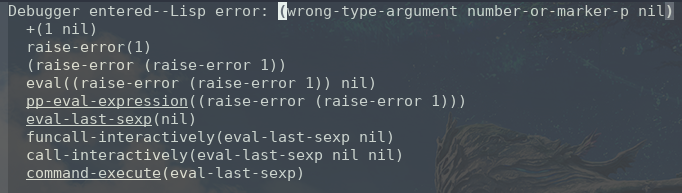
\includegraphics[width=.9\linewidth]{../../../files/raise-error.png}
\caption{报错的时候}
\end{figure}

上面可以看到一些行的前面有些"单词"会画上下划线,那些都是 \texttt{Lisp} 定义的函数或者宏,也是执行时候所调用的内容,从下往上看就是调用顺序.

调试的时候可以根据这个"大纲"来快速定位问题发生的位置.

\begin{verbatim}
(defun no-error (a)
  (+ a 1))

(debug-on-entry 'no-error)

(no-error (no-error 1))
\end{verbatim}


\begin{figure}[htbp]
\centering
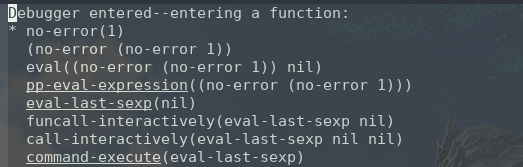
\includegraphics[width=.9\linewidth]{../../../files/no-error.png}
\caption{没有错误的时候}
\end{figure}

两者的提示是不一样的,除此以外,有一些命令在报错的时候是不可以执行的.比如 \texttt{r} 命令就不可以,因为错误是不能返回的.

调试器本身一定要经过编译运行,因为需要假设调试器自身需要使用多少个栈帧.如果是直译运行调试器,假设就会失败.


\item 调试器命令 (Debugger Commands)
\label{sec:org157e337}

如果能理解 \textbf{Emacs Lisp的调试器是一个递归编辑,每一个进入栈帧都是进入一个子调试器},文档上的说明就很好理解.尽管如此我还是要用自己的话总结一下(我没有了解以前可是一头雾水).

\begin{itemize}
\item c: 执行并且退出当前栈帧的调试,在下一个星号标记的栈帧处停止.
\item d: 进入当前栈帧并且给该栈帧添加星号, \texttt{debug-on-entry} 实际上就是给指定的函数添加星号.进入后可以通过c命令跳出.
\item b: 给当前栈帧添加星号.
\item u: 取消当前栈帧的星号.
\item j: 给当前栈帧添加星号然后和c命令一样执行,不过会无视 \texttt{debug-on-entry} 设定的星号(或者说临时禁止所有函数的break-on-entry). \texttt{c} 和 \texttt{j} 的区别可以通过调试上面没有错误的例子来了解一下.
\item e: 在 \texttt{minibuffer} 读取 \texttt{Lisp} 表达式并且(如果可以的划在当前词法环境)进行运算以及在回显区域(area echo)打印结果.调试器会在外部临时储存和恢复运行时变量值,所以可以随意检查和更改运行时的值.
\item R: 和e命令一样,不同的是R命令会储存计算结果到 \texttt{*Debugger-record*}.
\item q: 终止调试器(最开始的调试器),返回 \texttt{Emacs} 的 \texttt{top-level}.
\item r: 在带星号的栈帧返回时指定它的返回值,用于 \texttt{mock}.
\item l: 显示一个函数列表,这些函数都是会唤醒调试器的.
\item v: 切换显示当前栈帧的本地变量.
\end{itemize}


\item 唤醒调试器 (Invoking the Debugger)
\label{sec:org5b88c08}

关于 \texttt{debug} 函数的细节.该函数的第一个参数可以用来改变 \texttt{*Backtrace*} 顶部的提示信息 "Debugger entered--XXX".具体看文档就好.


\item 调试器内部 (Internals of Debugger)
\label{sec:org308d0f3}

关于调试器内部使用的函数和变量.

\begin{itemize}
\item \texttt{debugger} 变量: 用来指定调用 \texttt{debug} 函数时候使用的参数,默认是 \texttt{debug},参考 \texttt{debug} 函数的细节, \texttt{M-: (info "(elisp) Internals of Debugger")}.
\item \texttt{backtrace} 函数: \texttt{debug} 函数使用该函数给 \texttt{*Backtrace*} 缓冲区填充,它是用C语言写的,因为必须要访问栈来判断函数调用是否 \texttt{active},返回值总是 \texttt{nil},该函数的输出默认到 \texttt{standard-output} 的.
\item \texttt{debug-on-next-call} 变量: \texttt{non-nil} 表示在下一个 \texttt{eval, apply 或者 funcall} 之前调用调试器,进入调试器后把它设置为 \texttt{nil}.调试器的d命令就是通过设置这个变量来工作.如果直接手动设置该变量会进入调试器,可以试试.
\item \texttt{backtrace-debug} 函数: 设置 \texttt{LEVEL} 级别的栈帧的 \texttt{debug-on-exit flag} 为 \texttt{FLAG}, \texttt{LEVEL} 和 \texttt{FLAG} 是函数的参数. \texttt{FLAG} 为 \texttt{non-nil} 则是说在当前栈帧结束后进入调试器.
\item \texttt{command-debug-status} 变量: 记录当前交互命令的调试状态,每一次交互式调用命令就会把这个变量绑定为 \texttt{nil}.调试器可以设置这个变量来给在调试时引发的新调试器调用(debugger invocation)留下信息.
\item \texttt{backtrace-frame} 函数: 返回第 \texttt{FRAME-NUMBER} 层级栈帧的信息.
\end{itemize}
\end{enumerate}


\subsubsection{使用 Edebug 调试}
\label{sec:org84e4b30}

与 \texttt{Debugger} 相比, \texttt{Edebug} 更加适合用于阅读源码, \texttt{Debugger} 更多是输出回溯(backtrace)信息来进行调试,

这意味着如果要查看某处代码的运行细节,就得在那部分代码抛出异常进入调试模式,具体操作是在代码处添加 \texttt{(debug)},

然而修改别人的库/代码可是不是一件好事.

\texttt{Edebug} 作为一个源码级调试器(source-level debugger) 可以在不修改原有代码的前提下逐步执行,观察执行过程.

\subsubsection{Edebug}
\label{sec:orgca6b6f8}

\texttt{Emacs Lisp} 的代码级调试(source-level debugger),比 \texttt{Debugger} 强大好多.

\begin{enumerate}
\item 使用Edebug (Using Edebug)
\label{sec:org903f455}

使用 \texttt{Edebug} 调试需要先 \texttt{instrument} \texttt{Lisp} 代码,最简单的做法就是把指针移动到函数或者宏的定义然后执行 \texttt{C-u C-M-x} ,也就是带前缀参数的 \texttt{eval-defun} 命令.

一旦完成,任何该函数/宏的调用就会激活 \texttt{Edebug},定义的源代码的缓冲区就会临时变成 \texttt{read-only},当行的左边会有一个箭头表示当前执行的行,然后就可以在上面执行调试命令.

和 \texttt{Debugger} 一样,每一个 \texttt{list} 表达式的前面和后面都是点,和变量引用的后面也是点, \texttt{Edebug} 可以在这些点上面停止执行,叫做停止点(stop points).

可以通过 \texttt{<SPC>} 来执行直到下一个停止点,当 \texttt{Edebug} 在一个表达式后面停止执行,就会在回显区域里面显示表达式的值.

其它常用命令有:

\begin{itemize}
\item b: 在停止点设置 \texttt{breakpoint}
\item g: 执行直到到达一个 \texttt{breakpoint}
\item q: 退出 \texttt{Edebug}
\item ?: \texttt{Edebug} 的帮助命令
\end{itemize}


\item Instrumenting
\label{sec:org58e569f}

\texttt{Instrumenting} 代码其实就是给源代码插入额外的代码(当然并没有修改源代码),用来在合适的地方唤醒 \texttt{Edebug}.

如果要移除代码的 \texttt{instrumentation},只要以不添加 \texttt{instrumentation} 的方式重新运行一遍就好了.(在 \texttt{instrumenting} 之后修改源代码会导致 \texttt{instrumentation} 失效).

如果接移除单个定义的 \texttt{instrumentation},可以在定义上面执行 \texttt{C-M-x},也就是 \texttt{eval-defun} 命令.

可以通过 \texttt{M-x edebug-all-defs} 来切换 \texttt{edebug-all-defs} 变量,该变量可以控制 \texttt{eval-defun} 是否使用前缀参数来 \texttt{instrument} 定义, \texttt{nil} 表示需要.

如果 \texttt{edebug-all-defs} 为 \texttt{non-nil},那么直接移除单个定义的 \texttt{instrumentation} 就需要 \texttt{C-u C-M-x},为 \texttt{non-nil} 时候还可以配合 \texttt{eval-region, eval-current-buffer 和 eval-buffers} 命令来批量 \texttt{instrument},

如果要批量移除 \texttt{instrumentations} 先把 \texttt{edebug-all-defs} 切换回去再次运行命令就可以了(可以用 \texttt{eval-buffer} 体验一下).

还有一个特定用来控制 \texttt{eval-region} 是否 \texttt{instrument} 的 \texttt{edebug-all-forms}.

\texttt{M-x edebug-eval-top-level-form} 会无视 \texttt{edebug-all-defs} 和 \texttt{edebug-all-forms} 的值来进行 \texttt{instrumenting}. \texttt{edebug-defun} 是它的别名.

当 \texttt{Edebug} 激活的时候,命令I (\texttt{edebug-instrument-callee}) 可以根据调用来 \texttt{instrument} 定义(当然只能是没有添加instrumentation的情况下).

比如,

\begin{verbatim}
(defun fac (n)
  (if (< 0 n)
      (* n (fac (1- n)))
    (return-res 1)))

(defun return-res (n)
  (+ n 0))

(fac 3)
\end{verbatim}

如果 \texttt{edebug} 激活了,上面 \texttt{instrument fac} 只会给 \texttt{fac} 添加 \texttt{instrumentation},调试的时候可以把指针移动到 \texttt{(return-res 1)} 的前面使用I命令,

这样在 \texttt{fac} 调用 \texttt{(return-res 1)} 的时候就会进入 \texttt{return-res} .当然只能在 \texttt{Edebug} 知道定义源代码位置的时候才可以使用这命令.

如果想直接跳进 \texttt{return-res},可以直接使用i命令,它会先是 \texttt{instrument} 定义并且直接跳转.

Edebug 知道如何 \texttt{instrument} 所有标准 \texttt{special forms},但是不能靠它自己判断用户定义宏(user-defined macro)的参数信息.

因此唯一通过使用 \texttt{Edebug specifications} 来提供信息.当 \texttt{Edebug} 第一次 \texttt{instrument} 代码,它会运行 \texttt{edebug-setup-hook} 钩子然后把这个钩子设置为 \texttt{nil},可以使用这个钩子提供 \texttt{Edebug specification}.


\item Edebug执行模式 (Edebug Execution Modes)
\label{sec:org4b89d50}

\texttt{Edebug} 有很多个执行模式,比如可以手动逐步执行,可以自动逐步执行,可以手动逐个断点执行,当然也可以自动逐个断点执行,甚至可以无视断点执行.

在两种情况下可以设定模式,分别是使用对应模式的命令来设定调试时的模式和设定调试开始时的模式.

文档没有明说, \texttt{Edebug} 和 \texttt{Debugger} 一样都是递归编辑,每运算一次表达式都是进入 \texttt{Edebug},自己要清楚这一点.

下面是命令,

\begin{itemize}
\item S: Stop,不再执行调试,等待调试命令.
\item \texttt{<SPC>}: Step,在下一个停止点处停止.
\item n: Next,在下一个表达式的后面的停止点处停止.
\item t: Trace,默认每一秒后运行到下一个停止点,就是 \texttt{<SPC>} 的自动模式.
\item T: Rapid trace, \texttt{t} 的快速执行模式,中间没有停顿.
\item g: Go,运行到下一个断点.
\item c: Continue,在每个断点处停留一秒,然后继续,就是 \texttt{g} 的自动模式.
\item C: Rapid continue: \texttt{c} 的快速执行模式,中间没有停顿.
\item G: Go non-stop,无视断点执行,可以通过 \texttt{S} 停止.
\end{itemize}

可以通过 \texttt{edebug-set-initial-mode} 命令设置 \texttt{edebug-initial-mode} 来设定 \texttt{Edebug} 的初始模式.

对于自动模式的停顿时间,可以通过设置 \texttt{edebug-sit-for-seconds} 变量来修改.


\item 跳转 (Jumping)
\label{sec:org54b4956}

跳转就是指执行到哪个停止点.命令如下,

\begin{itemize}
\item h: 执行到下一个断点.
\item f: 执行完一个表达式.
\item o: 执行完一个 \texttt{containing sexp},也就是跳出(step out).
\item i: 跳进一个停字点后面函数或者宏(step in).
\end{itemize}

具体说明还是看文档吧.


\item Edebug 的杂项命令 (Edebug Misc)
\label{sec:org5475ff9}

\begin{itemize}
\item ?: 帮助命令.
\item C-]: 终止(abort)一个 \texttt{level} 返回到上一个 \texttt{command level}.
\item q: 返回到 \texttt{top level},也就是停止 \texttt{edebug} 调试器.然而,被 \texttt{unwind-protect} 或者 \texttt{condition-case} 保护的 \texttt{instrumented code} 会恢复 \texttt{edebug}.
\item Q: 像 \texttt{q} 一样,不过无视被保护的代码.
\item r: 重新显示最近的表达式的结果.
\item d: 显示 \texttt{backtrace},这个 \texttt{backtrace} 不像标准的 \texttt{Debugger} 那样执行命令.继续执行的时候会自动关闭 \texttt{backtrace}.
\end{itemize}


\item 中断 (Breaks)
\label{sec:orga448271}

一旦 \texttt{Edebug} 开始,除了 \texttt{step mode} 可以在下一个停止点停止执行,还有其它三种方法可以停止执行.

\begin{enumerate}
\item 断点 (Breakpoints)
\label{sec:orgc267c9f}

可以在任何一个停止点设置断点.关于断点的命令如下:

\begin{itemize}
\item b: 在停止点设置断点.如果使用了前缀参数,断点就是临时的,停止调试后断点就失效了.
\item u: 取消断点.
\item \texttt{x CONDITION <RET>}: 条件断点,只有 \texttt{CONDITION} 结果为 \texttt{non-nil} 才会停止.同样,如果使用了前缀参数的话就是临时的.
\item B: 移动到当前定义的下一个断点.
\end{itemize}

\item 全局中断条件 (Global Break Condition)
\label{sec:org129dbad}

全局中断条件不管在哪里,只要条件符合就停止调试的执行. \texttt{Edebug} 会在每个停止点运算全局中断条件的值,如果结果为 \texttt{non-nil} 就停止或者暂停执行,和断点一样.然而如果运行条件的时候报错是不会停止.

条件表达式储存在 \texttt{edebug-global-break-condition} 变量里面.可以在已经激活了 \texttt{Edebug} 的源代码缓冲区中使用X命令来添加条件表达式,也可以使用 \texttt{C-x X X} 按键(绑定 \texttt{edebug-set-global-break-condition})在任何缓冲区中添加条件表达式.

全局中断条件很容易让调试变慢,如果不使用的话要把 \texttt{edebug-global-break-condition} 设置为 \texttt{nil}.

\item 源码断点 (Source Breakpoints)
\label{sec:org194de51}

上面通过b命令设置的断点会在 \texttt{reinstrument} 定义后被遗忘(除了Emacs,人也可能会忘记),这个时候可以使用"源码断点"(和 \texttt{Debugger} 的 \texttt{(debug)} 的用法一样).

在想要断点的地方插入 \texttt{(edebug)} 表达式,如果定义没有被 \texttt{instrument},那么遇到 \texttt{(edebug)} 就会转而调用 \texttt{debug} 函数.可以使用g命令跳转到这种断点身上.
\end{enumerate}


\item 捕捉错误 (Trapping Errors)
\label{sec:org7576c47}

设置 \texttt{edebug-on-error} 或者 \texttt{edebug-on-quit} 可以快速定位没有被处理错误(unhandled errors),就拿 \texttt{edebug-on-error} 来说,它和 \texttt{debug-on-error} 的设置类似,用下面的例子来演示.

\begin{verbatim}
(setq edebug-on-error t)

;; 当然要先 instrument fac 的定义,这是必须的
(defun fac (n)
  (if (< 0 n)
      (* n (fac (1- n)))
    (return-res nil))) ; 错误在这里,会在 (return-res nil)前面的停止点停下

(defun return-res (n)
  (+ n 0))

(fac 3)
\end{verbatim}

在这个例子中可以使用 \texttt{Rapid Trace} 模式来直接运行到错误发生的地方,会发生和注释一样的结果.如果把 \texttt{edebug-on-error} 设置为 \texttt{nil},是不会停止到错误发生的地方,而是直接在回显区域显示信息.


\item Edebug Views
\label{sec:org914f5c8}

一些用来浏览已经激活 \texttt{Edebug} 的缓冲区和窗口状态的各个方面.

外部窗口配置(outside window configuration) 集合了窗口(windows)和在 \texttt{Edebug} 外部有效(in effect)的内容(个人认为像是发生调用的地方).

\begin{itemize}
\item v: 切换到外部窗口配置中.
\item p: 临时切换到等待 \texttt{N} 秒(可以通过 \texttt{C-u N p} 设定暂停时间)后返回 \texttt{Edebug} 中.
\item w: 把点(point)返回到到源码缓冲区当前的停止点上.
\item W: 切换是否保存和恢复外部窗口配置,有前缀参数的话就表明只是对被选择窗口切换是否保存和恢复.
\end{itemize}


\item 运算 (Edebug Eval)
\label{sec:orgfc2c140}

当 \texttt{Edebug} 启用的时候,你可以像在没有运行 \texttt{Edebug} 的情况下运算表达式.

\begin{itemize}
\item \texttt{e EXP <RET>},在 \texttt{Edebug} 外部的上下文运算表达式 \texttt{EXP}.这样 \texttt{Edebug} 可以减少它和运算之间的冲突/干扰(interference).

\item \texttt{M-: EXP <RET>},在 \texttt{Edebug} 的上下文中运算表达式 \texttt{EXP}.

\item \texttt{C-x C-e},在 \texttt{Edebug} 外面运算点之前表达式.
\end{itemize}

\texttt{Edebug} 支持运算引用由 \texttt{cl.el} 里面 \texttt{lexical-let, macrolet} 和 \texttt{symbol-macrolet} 词法绑定的 \texttt{symbols} 的表达式.


\item 运算列表缓冲区 (Eval List)
\label{sec:org5d95f89}

可以使用运算列表缓冲区(evaluation list buffer),叫做 \texttt{*edebug*} 的缓冲区,来交互运算表达式.也可以设置表达式的运算列表(evaluation list),这样它们在每次 \texttt{Edebug} 更新显示的时候都会更新.

在 \texttt{Edebug} 激活之后使用 \texttt{E} 命令切换到运算列表缓冲区 -- \texttt{*edebug*},然后在里面添加元素表达式组(evaluation list groups).一个运算表达式组包含一到多条表达式,用注释行(comment lines)分组,如下

\begin{verbatim}
(point)
                                        ; whatever comment you like, but the ';' must be without any prefix.
this-command
                                        ;
undefined
                                        ;
\end{verbatim}

再使用 \texttt{C-c C-u} 根据 \texttt{*edebug*} 缓冲区的内容建立新的运算列表(evaluation list),结果如下

\begin{verbatim}
(point)
264
                                        ;------------------------------------------------------------------------------------------------------
this-command
eval-last-sexp
                                        ;------------------------------------------------------------------------------------------------------
undefined
"Symbol's value as variable is void: undefined"
                                        ;------------------------------------------------------------------------------------------------------
\end{verbatim}

使用 \texttt{C-c C-u} 运算的话,只有每个组的第一条表达式会执行,结果会显示在第二行,其它行会被删除.如果运算时候发生错误,那么错误信息就会作为结果.

还可以把指针移动到组内然后使用 \texttt{C-c C-d} 删除分组.

除了 \texttt{C-c C-u},还有其它运行模式,看文档就好.


\item Edebug 的打印 (Printing in Edebug)
\label{sec:orgc31eb54}

如果尝试在 \texttt{Edebug} 中打印一个包含循环列表结构的值,那么可能会发生错误.

克服(cope with)循环结构的一个方法就是把 \texttt{print-length} 或者 \texttt{print-level} 来分断显示. \texttt{Edebug} 已经帮你做好了.

它把这两个变量分别绑定到 \texttt{edebug-print-length} 和 \texttt{edebug-print-level},默认值都是50.

也可以通过设置 \texttt{print-circle} 为 \texttt{non-nil} 来打印那种有着共享元素的循环结构体.

比如

\begin{verbatim}
(setq a '(x y))
(setcar a a)
;; 显示为 #1=(#1# y), #1= 表示用1标记结构,#1#表示引用前一个被标记的结构.这个标记可以用在任何列表或者向量的共享元素上.
\end{verbatim}

相应的 \texttt{Edebug} 有 \texttt{edebug-print-circle},会把这个变量的值绑定给 \texttt{print-circle}.


\item 运行步骤缓冲区 (Trace Buffer)
\label{sec:org25f2ffe}

\texttt{Edebug} 可以把执行步骤记录在叫做 \texttt{*edebug-trace*} 的缓冲区中,一个函数调用和返回的日志,显示函数的名字和它们的参数和值.只要把 \texttt{edebug-trace} 设置为 \texttt{non-nil} 就可以启用该功能.

比如上面 \texttt{fac} 的记录会是这样,

\begin{verbatim}
{ fac args: (3)
:{ fac args: (2)
::{ fac args: (1)
:::{ fac args: (0)
:::} fac result: 1
::} fac result: 1
:} fac result: 2
} fac result: 6
\end{verbatim}

\texttt{\{} 和 \texttt{\}} 分别表示函数的入口和出口, \texttt{:} 表示递归深度,同一深度的 \texttt{\{} 对应同样深度的 \texttt{\}}.可以通过重新定义 \texttt{edebug-print-trace-before} 和 \texttt{edebug-print-trace-after} 函数来自定义记录函数入口和出口显示的条目.

\texttt{edebug-tracing} 和 \texttt{edebug-trace} 函数在 \texttt{*edebug*} 中插入行,不管是否启用 \texttt{Edebug}.插入行也会自动滚动窗口来显示最新行.


\item 覆盖测试 (Coverage Testing)
\label{sec:org2ea4a30}

\texttt{Edebug} 还提供不完全的覆盖参数和执行频次(execution frequency)的显示.

\textbf{覆盖参数的原理就是比较每个表达式的当前结果和上一次结果,如果返回的两个结果不一样,这个表达式被覆盖了}.

覆盖参数就是需要在大量的各种不同条件下执行程序,并且观察程序是否符合预期, \texttt{Edebug} 会在足够的尝试后告诉开发人员是否每个 \texttt{form} 返回两个不同结果.

覆盖测试会让执行变慢, \texttt{edebug-test-coverage} 为 \texttt{non-nil} 的时候测试所有被调试的表达式.

不管是否启用了覆盖测试或者是否 \texttt{Go-nonstop} 执行模式, \texttt{instrumented function} 的所有执行都会伴随频次计数(frequency counting)的执行.

"C-x X =" (edebug-display-freq-count) 可以显示一个定义的覆盖信息和频次计数. 单纯 = (edebug-temp-display-freq-count) 会临时显示同样的信息,知道输入了另外一个按键.

还是用那个老例子说明,当然还有先 \texttt{instrument fac}.

\begin{verbatim}
(setq edebug-test-coverage t)

;; 1. instrument
;; 3. move cursor on definition and execute edebug-display-freq-count command
(defun fac (n)
  (if (< 0 n)
      (* n (fac (1- n)))
    (return-res 1)))

(defun return-res (n)
  (+ n 0))

;; 2. then execute, can use Rapid Trace mode for a quick travel
(fac 5)
\end{verbatim}

\texttt{edebug-display-freq-count} 的用法: 先调试运行一遍(否则全部数据为0),然后把指针移动到 \texttt{instrumentd} 定义中,然后执行该命令显示覆盖信息和执行频次.

结果如下,

\begin{verbatim}
(setq edebug-test-coverage t)

;; 1. instrument
;; 3. move cursor on definition and execute edebug-display-freq-count command
(defun fac (n)
  (if (< 0 n)
                                        ;#6
      (* n (fac (1- n)))
                                        ;#    5
    (return-res 1)))
                                        ;#  1            = 6

(defun return-res (n)
  (+ n 0))

(fac 5)
\end{verbatim}

执行频次会出现在表达式前面的 \texttt{(} ,后面的 \texttt{)} 或者是变量最后一个字母的底下.为了简化显示,如果表达式的频次计数等于同一行中前一个表达式的频次,那么这个频次就不显示.

跟在频次计数后面的 "=" 号表示表达式每次执行结果都是一样,也就是该表达式没有被覆盖.

再以文档上的例子来做说明,

\begin{verbatim}
(defun fac (n)
  ;; (edebug) 只是返回了一次,不算覆盖.
  ;; (if (= n 0) ... 执行了6次,每次结果都是 =nil=.
  ;; = 和频次计数是没有关系的,切记.
  (if (= n 0) (edebug))
                                        ;#6           1      = =6
  ;; (< 0 n) 和 (if (< 0 n) ... 的执行频次都是一样,所以 (< 0 n) 没有显示频次
  ;; (< 0 n) 每次的结果都为 t,
  (if (< 0 n)
                                        ;#6
      ;; (* n (fac ...  以及它的子表达式的执行频次都是一样的(并且都在同一行),所以简化显示只显示了第一个表达式的执行频次.
      (* n (fac (1- n)))
                                        ;#    5
    1))
                                        ;#   6

(fac 5)
\end{verbatim}

还可以在 \texttt{Edebug} 调试中的时候使用 = 命令临时显示覆盖信息和频次计数.


\item 外部上下文 (The Outside Context)
\label{sec:org73642fe}

对于调试中的程序来说, \texttt{Edebug} 尝试变得透明,然而没完全成功.也尝试过在我们运行e命令或者使用运算列表缓冲区的时候通过临时恢复外部上下文来变得透明.

这个章节主要介绍 \texttt{Edebug} 储存什么上下文并且为什么完全透明.

\begin{enumerate}
\item 检查是否停止 (Checking Whether to Stop)
\label{sec:org9afb4fb}

当进入 \texttt{Edebug} 的时候,它在决定是否产生执行信息(trace information)或者停止程序之前就需要储存和恢复一定的数据.

\begin{itemize}
\item 增加 \texttt{max-lisp-eval-depth} 和 \texttt{max-specpdl-size} 都可以减少 \texttt{Edebug} 对栈的影响.不过这样很容易用完栈的空间.

\item 键盘宏的执行状态回被保存和恢复.当 \texttt{Edebug} 激活的时候, \texttt{executing-kbd-macro} 会设置为 \texttt{nil}, 除非 \texttt{edebug-continue-kbd-macro} 为 \texttt{non-nil}.
\end{itemize}

\item Edebug显示更新 (Edebug Display Update)
\label{sec:org6143a97}

当 \texttt{Edebug} 需要显示一些信息的时候,它会储存 \texttt{Edebug} 外部的当前窗口配置.当退出 \texttt{Edebug} 的时候它就会恢复之前的窗口配置.

只有在 \texttt{Edebug} 暂停的时候 \texttt{Emacs} 才会重新显示(\texttt{redisplay}).通常,当继续执行的时候,程序会在断点处或者单步执行(stepping)后重新进入(re-enter) \texttt{Edebug},中间没有任何停顿或者输入读取.

在这写例子中, \texttt{Emacs} 没有任何机会重新显示外部配置.因此,你所看见的就是和最后一次激活 \texttt{Edebug} 时的同一个窗口配置,没有任何中断(interruption).

用于显示信息的 \texttt{Edebug} 入口也会储存和恢复以下数据(尽管它们中的一些会因为 \texttt{error and quit signal} 的发生而有意不储存).

\begin{itemize}
\item 当前的缓冲区,点的位置(point positions),marks和已经被储存的和恢复的数据.

\item 如果 \texttt{edebug-save-windows} 是 \texttt{non-nil},那么外部窗口配置就会被储存和恢复.不会在 \texttt{error} 或者 \texttt{quit} 的时候恢复,不过即使 \texttt{save-excursion} 激活时候出现了 \texttt{error} 或者 \texttt{quit},外部被选中的窗口还是会被重新选择.

如果 \texttt{edebug-save-windows} 是一个列表,只有被列出的窗口会被储存和恢复.窗口开始以源代码缓冲区的水平滚动位置是不会储存的.然而,它们仍然会被保留并且显示在 \texttt{Edebug} 中.

\item 如果 \texttt{edebug-save-displayed-buffer-points} 为 \texttt{non-nil},那么每个显示的缓冲区的点都会被保留和恢复.

\item \texttt{overlay-arrow-position} 和 \texttt{overlay-arrow-string} 会被储存和恢复,因此可以安全地从在同一个缓冲区中任何地方的递归编辑(recursive edit)唤醒 \texttt{Edebug}.

\item \texttt{cursor-in-echo-area} 局部绑定 \texttt{nil},这样指针(cursor)会显示到窗口上.
\end{itemize}

\item Edebug Recursive Edit
\label{sec:org2de2ce5}

当进入 \texttt{Edebug} 并且读取命令时,会储存和之后恢复以下额外的数据.

\begin{itemize}
\item 当前的匹配数据(Match Data)

\item \texttt{last-command, this-command, last-command-event, last-input-event, last-event-frame, last-nonmenu-event and trace-mouse}. \texttt{Edebug} 的命令不会在 \texttt{Edebug} 之外影响它们.

\texttt{Edebug} 的执行命令可以改变 \texttt{this-command-keys} 返回 \texttt{key sequence},并且没有办法从 \texttt{Lisp} 中重置.不能储存和恢复 \texttt{unread-command-events} 的值.

\item \texttt{command-history} 记录着 \texttt{Edebug} 中执行的命令,在北少数情况下这个可以修改执行(execution).

\item \texttt{Edebug} 中的递归深度比外部的递归深度要深,当时对于自动更新的运算列表窗口来说是错的.

\item \texttt{standard-output} 和 \texttt{standard-input} 会被 \texttt{recursive-edit} 命令绑定为 \texttt{nil},不过 \texttt{Edebug} 会在运算中临时恢复它们.

\item 键盘宏的定义的状态会被保存和恢复.当激活 \texttt{Edebug} 时, \texttt{defining-kbd-macro} 会绑定到 \texttt{edebug-continue-kbd-macro}.
\end{itemize}
\end{enumerate}


\item Edebug and Macros
\label{sec:org1280493}
\begin{enumerate}
\item Instrumenting Macro Calls
\label{sec:orgec25c1d}

当 \texttt{Edebug} \texttt{instrument} 一个调用 \texttt{Lisp} 宏的表达式,它需要额外的宏信息来保证正确工作.

那是因为没有一个先验 (\texttt{a-priori})的方法来判断会运算宏调用的哪些子表达式(宏体可能会发生运算,或者拓展时候发生运算,又或者之后任何时刻).

因此必须为每一个 \texttt{Edebug} 会遇到的宏定义 \texttt{Edebug specification} 来解释宏的调用格式.做法是给宏定义添加一个 \texttt{debug} 声明.

\texttt{Edebug specification} 告诉 \texttt{Edebug} 宏的哪些部分需要运算.关于如何为宏定义 \texttt{Edebug specification},看这里 \texttt{M-: (info "(elisp) Defining Macros")}.

当 \texttt{instrument} 代码的时候要保证 \texttt{Edebug} 知道 \texttt{specification}.如果 \texttt{instrument} 一个文件中的函数,并且这个函数引用了使用 \texttt{eval-when-compile} 导入另外一个文件的宏定义,那么就需要 \texttt{load} 一遍那个文件.

除了上面的方法外,还可以使用 \texttt{def-edebug-spec} 为宏定义 \texttt{Edebug specification}.添加 \texttt{debug} 更受欢迎以及更方便.不过 \texttt{def-edebug-spec} 可以为 \texttt{C} 实现的 \texttt{special forms} 定义 \texttt{Edebug specifications}.

如果一个宏没有 \texttt{Edebug specification}, \texttt{edebug-eval-macro-args} 就会参与进来,如果该变量为 \texttt{nil} (默认),运算的时候不会为任何一个参数 \texttt{instrument};否则全员 \texttt{instrumented}.

\item Specification List
\label{sec:org8c1ab1c}

自己看文档

\item Backtracking
\label{sec:org9704762}

自己看文档

\item Specification Examples
\label{sec:org35e6d13}

自己看文档
\end{enumerate}


\item Edebug Options
\label{sec:org4c0405c}

大部份上面都提过,自己看文档
\end{enumerate}


\subsubsection{语法错误 (Syntax Errors)}
\label{sec:orgb8061b0}

\texttt{Lisp reader} 会提示非法语法,不过不会提示问题发生的地方.对于 \texttt{Lisp} 来说,最常见的语法错误就是括号不匹配.

\begin{enumerate}
\item 多余的开括号 (Excess Open)
\label{sec:org199773d}

多余开括号的错误提示是 \texttt{End of file during parsing}.

\begin{enumerate}
\item 移动指针到发生错误的文件的最后执行 \texttt{C-u C-M-u},以此找到错误的函数.

\item 研究错误的函数,可以根据现有的缩进来判断.

\item 保证函数的定义有足够的闭括号(一般都是先移动到函数的结尾插入一个闭括号,不要使用 \texttt{C-M-e} 移动,括号不平衡时会报错),否则 \texttt{C-M-q} 会报错或者重新缩进到文件最后.

\item 移动到函数定义的开始处使用 \texttt{C-M-q} 来重新缩进并且过程哪部分发生右动,通常发生右偏移的起点的前一个点的附近就是少了闭括号或者多了开括号的地方(当然这不一定是对的).一定要细读代码.

\item 一旦找到了就用 \texttt{C-\_} 撤销(undo) \texttt{C-M-q},恢复到旧的缩进.

\item 再次移动到函数定义的起点执行 \texttt{C-M-q} 来检查缩进是否正常,如果缩进没有发生改变就证明括号匹配了.
\end{enumerate}


\item 多余的闭括号 (Excess Close)
\label{sec:orgacb1796}

多余闭括号的错误提示是 \texttt{Invalid read syntax: ")"}.

\begin{enumerate}
\item 移动指针到发生错误的文件的起点执行 \texttt{C-u -1 C-M-u} 查找第一个括号不平衡的函数.

\item 在函数定义的起点使用 \texttt{C-M-f} 来匹配闭括号,执行让指针移动到定义应该结束的地方.很有可能就找到多余的闭括号.

\item 如果上面还没有找到问题,那么就在函数的定义起点执行 \texttt{C-M-q} 进行缩进并且观察哪部分移动,通常发生左偏移的起点的前面一个点的附近就是多了闭括号或者少了开括号的地方(当然这不一定是对的).一定要细读代码.

\item 一旦找到了就用 \texttt{C-\_} 撤销 \texttt{C-M-q},恢复到旧缩进.

\item 再次移动到函数定义的起点执行 \texttt{C-M-q} 来检查缩进是否正常,如果缩进没有发生改变就证明括号匹配了.
\end{enumerate}
\end{enumerate}


\subsubsection{覆盖参数 (Test Coverage)}
\label{sec:org0e0e9d2}

除了 \texttt{Edebug} 可以做覆盖参数,还可以使用 \texttt{testcover} 库来做.

\begin{enumerate}
\item \texttt{M-x testcover-start <RET> FILE <RET>} 对整个文件进行 \texttt{instrument}.

\item 调用一到多次来测试代码.

\item \texttt{M-x testcover-mark-all} 高亮覆盖率低的代码.

\item \texttt{M-x testcover-next-mark} 移动到下一个高亮点(next highlighted spot).
\end{enumerate}

关于高亮的说明,

\begin{itemize}
\item 红色(red)高亮点是指 \texttt{form} 完全没被执行过.如果 \texttt{forms} 不能完成运行就会跳过红色高亮,比如 \texttt{error}.

\item 棕色(brown)高亮点是指 \texttt{form} 总是运行得到相同结果.如果 \texttt{forms} 是本来就是预期得到相同的值就跳过棕色高亮,比如 \texttt{(setq x 14)}.
\end{itemize}

\texttt{testcover} 库还可以提供 \texttt{1value} 和 \texttt{noreturn} \texttt{form} 来在特定情况下使用.


\subsubsection{性能测试 (Profiling)}
\label{sec:org5fa8c4b}

针对不同情况有以下4种方法可以测试性能,

\begin{enumerate}
\item \texttt{Emacs} 的内置支持

\begin{itemize}
\item 步骤

\begin{enumerate}
\item \texttt{M-x profiler-start} 开始测试,可以选择测试的指标 \texttt{(cpu, mem, cpu+mem)}.

\item 做想要测试的动作.

\item \texttt{M-x profiler-report} 显示测试结果.

\item 结束后关闭测试 \texttt{M-x profiler-stop}.
\end{enumerate}

\item 如何读懂结果

\begin{figure}[htbp]
\centering
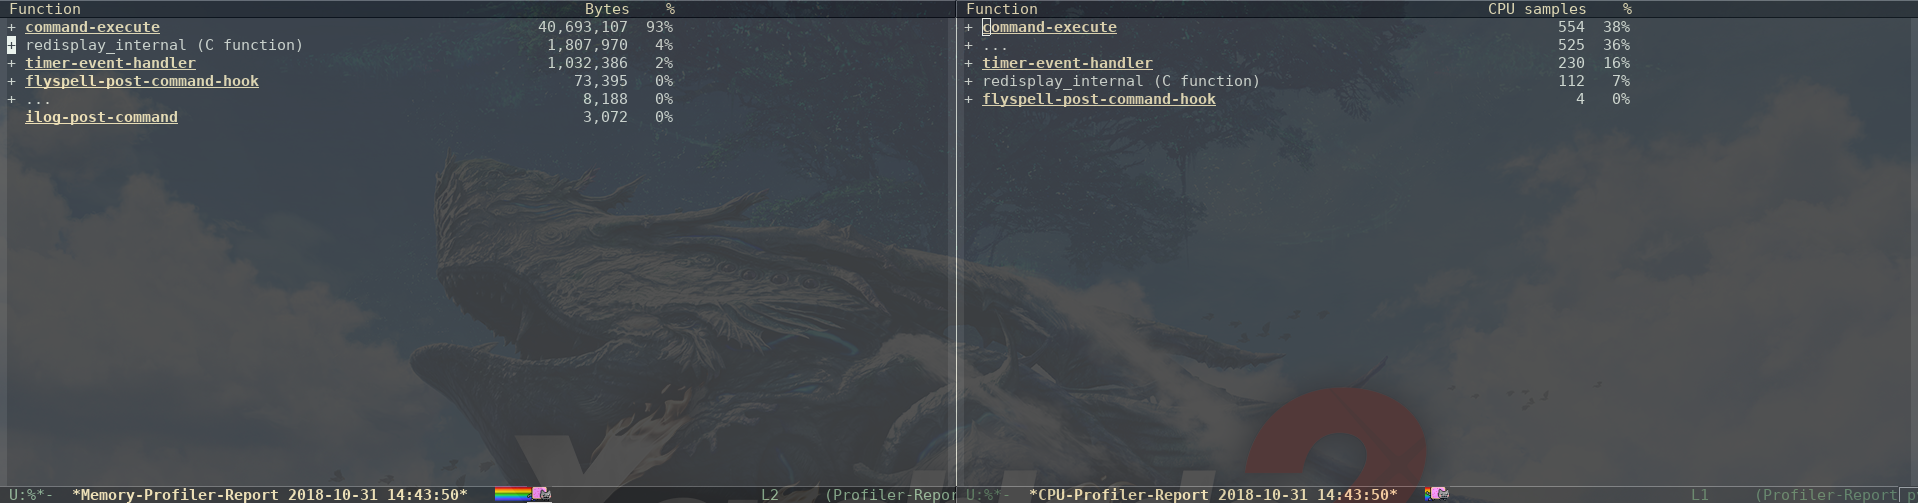
\includegraphics[width=.9\linewidth]{../../../files/cpu-mem.png}
\caption{cpu+mem usage}
\end{figure}

上面的图里分别是内存和cpu的使用率.

每一行的内容项分别为 \textbf{调用的函数名字}, \textbf{函数的资源使用} 以及 \textbf{函数执行时间占总测试时间的百分比}.

如果行的左边有 \texttt{+} 号,那么可以对着行输入 \texttt{<RET>} 进行展开,里面有这一行函数调用的 \texttt{subroutines}.可以通过 \texttt{C-u <RET>} 一次展开,再次 \texttt{<RET>} 可以再次折叠.

可以使用 \texttt{j} 或者 \texttt{mouse-2} 跳转到函数的定义.

使用 \texttt{d} 显示函数的文档.

使用 \texttt{C-x C-w} 保存测试结果.

使用 = 对比两份测试结果.
\end{itemize}

\item \texttt{elp} 库

可以做为 \texttt{profile} 的替代方案.

\item \texttt{bechmark} 库

使用 \texttt{benchmark-run} 和 \texttt{benchmark-run-compiled} 单独测试 \texttt{Emacs Lisp forms}.

\item 调试 \texttt{C} 实现的功能

需要在 \texttt{Emacs} 编译的时候启用 \texttt{configure} 选项的 \texttt{-{}-{}enable-profiling},

完成后会生成一份 \texttt{gmon.out} 文档,可以使用 \texttt{Linux} 的 \texttt{gprof} 命令来检测.

该特性主要用来调试 \texttt{Emacs} 的,并且会停止上面描述的 \texttt{Lisp-level} \texttt{M-x profiler-...} 命令.
\end{enumerate}



\subsubsection{ERT: Emacs Lisp Regression Testing}
\label{sec:org01f1f9c}

文档位于 \texttt{M-: (info "ert")}.

\texttt{ERT} 是 \texttt{Emacs Lisp} 的一个自动化测试库.主要功能有测试定义,运行测试,输出测试结果以及交互调试测试错误(debugging for test failures).

\textbf{交互调试测试错误这个真的是好东西}.

事实上 \texttt{ERT} 还适用于测试驱动开发(Test-driven development)模式和传统软件开发模式.

\begin{enumerate}
\item 简介 (Introduction)
\label{sec:org7db49bb}

\texttt{ERT} 允许组合函数,宏,变量以及其它 \texttt{Lisp} 的东西(construct)来定义测试(tests).测试只不过是调用其它的代码并且检查它们是否与期望的行为一样的 \texttt{Lisp} 代码.

\texttt{ERT} 会跟踪定义的测试和提供一些运行测试的命令,用于检测定义是否通过测试.

比如 \texttt{pp.el} 的文档中有这么一些测试用例,

\begin{verbatim}
;; (pp-to-string '(quote quote))          ; expected: "'quote"
;; (pp-to-string '((quote a) (quote b)))  ; expected: "('a 'b)\n"
;; (pp-to-string '('a 'b))                ; same as above
\end{verbatim}

用 \texttt{ERT} 写对应上面测试就是这样,

\begin{verbatim}
(ert-deftest pp-test-quote ()
  "Tests the rendering of `quote' symbols in `pp-to-string'."
  (should (equal (pp-to-string '(quote quote)) "'quote"))
  (should (equal (pp-to-string '((quote a) (quote b))) "('a 'b)\n"))
  (should (equal (pp-to-string '('a 'b)) "('a 'b)\n")))
\end{verbatim}

\texttt{ert-deftest} 和 \texttt{defun} 的用法比较像,定义一个名字叫 \texttt{pp-test-quote} 单元测试,加载后可以使用 \texttt{M-x ert <RET> t <RET>} 来运行测试.

如果三个调用结果全员 \texttt{non-nil} 的话,测试就通过.上面的 \texttt{should} 宏就是 \texttt{ert} 版本的断言语句(assertion).

每个测试应该有一个用来描述测试功能的名字,比如上面的 \texttt{pp-test-quote} 就是测试 \texttt{quote},测试的名字不会和函数和变量放在同一个命名空间,所以可以随意选择(还是要符合 \texttt{Emacs Lisp} 的规范,加上前缀表明属于哪一个包).

当测试不通过, \texttt{ERT} 就会显示测试的名字,还有测试的时候可以根据名字选择测试.

第一行的 \texttt{()} 目前没有任何意义,以后可能会用它来做拓展,同时也是为了接近 \texttt{defun} 的写法.

文档 (\texttt{docstring}) 用来描述所测试的功能点(feature).在交互测试中,如果测试失败,文档的第一行会被显示出来,当然文档是可选的.

测试体,也就是里面那三个表达式,可以是任何 \texttt{Lisp} 代码,可能的话可以有副作用,如果有,不论测试是否通过,应该完成后进行清理,还原成测试之前的状态.


\item 如何运行测试 (How to Run Tests)
\label{sec:org199125e}

有两种运行方式,第一种是在启动 \texttt{Emacs} 后交互运行,也就是上面章节提到的方法;第二种就是在命令行中运行,也就是 \texttt{batch mode}.

前者比较方便,后者可以与用户的自定义独立开;并且允许从 \texttt{makefiles} 中读取测试并且运行,能够根据不同版本的 \texttt{Emacs} 编写测试.

\begin{enumerate}
\item 交互运行测试 (Running Tests Interactively)
\label{sec:orgf13b6bf}

使用 \texttt{M-x ert <RET> t <RET>} 来运行所有已经加载了的测试.其中 \texttt{t} (也可以是字符串)是测试选择器(test selectors),还有别的选择器可以选.

假设现有测试如下,

\begin{verbatim}
(ert-deftest pp-test-quote ()
  "Tests the rendering of `quote' symbols in `pp-to-string'."
  (should (equal (pp-to-string '(quote quote)) "'quote"))
  (should (equal (pp-to-string '((quote a) (quote b))) "('a 'b)\n"))
  (should (equal (pp-to-string '('a 'b)) "('a 'b)\n")))

(ert-deftest addition-test ()
  "Addition"
  (should (equal (+ 1 2) 4)))
\end{verbatim}

其中 \texttt{addition-test} 是注定测试不通过的,

\begin{verbatim}
Selector: t
Passed:  1
Failed:  1 (1 unexpected)
Skipped: 0
Total:   2/2

Started at:   2018-11-01 00:00:17+0800
Finished.
Finished at:  2018-11-01 00:00:17+0800

F.

F addition-test
    Addition
    (ert-test-failed
     ((should
       (equal
        (+ 1 2)
        4))
      :form
      (equal 3 4)
      :value nil :explanation
      (different-atoms
       (3 "#x3" "?")
       (4 "#x4" "?"))))
\end{verbatim}

上面运行了两个测试,其中 \texttt{addition-test} 失败了,另外一个测试通过. \texttt{F} 和 \texttt{.} 分别表示一个失败的测试和一个通过的测试.

上面的 \texttt{:form} 指的是 \texttt{(equal (+ 1 2) 4)} 化简(reduced to)的结果,为 \texttt{(equal 3 4)}, \texttt{:value} 是 \texttt{(} 3 4)= 的结果.

和上面显示的一样,失败的测试会显示出细节,其中 \texttt{:explanation} 叫做解释 (Explanation). \texttt{M-: (info "(ert) Understanding Explanations")} 有关于如何理解解释.

在测试结果的缓冲区中,可以做以下命令,

\begin{itemize}
\item \texttt{TAB} 和 \texttt{S-TAB} 在按钮之间循环,函数和宏就是按钮.

\item \texttt{RET} 在按钮处跳转到按钮的定义.

\item \texttt{r} 重新运行指针附近的测试.

\item \texttt{d} 使用调试器重新运行.

\item \texttt{.} 跳转到点附近函数或者宏的定义,和 \texttt{RET} 差不多.

\item \texttt{b} 显示失败测试的 \texttt{backtrace}.

\item \texttt{l} 显示测试中的 \texttt{should} forms.

\item \texttt{m} 假如测试中使用了 \texttt{message} 函数产生信息,可以使用该命令进行显示.

\item \texttt{L} 失败测试的显示的表达式会根据 \texttt{print-length} 和 \texttt{print-level} 进行简短化.该命令可以增加显示限制.
\end{itemize}


\item 以 Batch Mode 运行测试 (Running Tests in Batch Mode)
\label{sec:orgca457ad}

可以从命令行或者脚本,又或者是 \texttt{makefiles} 自动运行测试.有两个函数可以做这件事情,分别是 \texttt{ert-run-tests-batch} 和 \texttt{ert-run-tests-batch-and-exit}.

在命令行下面可以这么用:

\begin{verbatim}
emacs -batch -l ert -l /path/to/tests.el -f ert-run-tests-batch-and-exit
\end{verbatim}

如果测试全员通过就返回 \texttt{0} 状态码,否则就是非 \texttt{0} 状态码.

还可以先把运行结果重定向到别的文件,比如 output.log,然后使用 \texttt{ert-summarize-tests-batch-and-exit} 产生总结信息,

\begin{verbatim}
emacs -batch -l ert -l tests.el -f ert-run-tests-batch-and-exit >& output.log
emacs -batch -l ert -f ert-summarize-tests-batch-and-exit output.log
\end{verbatim}

如果 \texttt{Emacs} 没有和 \texttt{ERT} 一起分发,那么需要 \texttt{-L /path/to/ert} 来先加载 \texttt{ert} 库,可能还需要用 \texttt{-L /path/to/tests.el} 来确保测试文件被加载.


\item 测试选择器 (Test Selectors)
\label{sec:orgb776f6e}

运行 \texttt{ert} 的时候需要选择测试选择器,也就是运行符合条件的测试.

\begin{itemize}
\item \texttt{nil},不选择任何测试.

\item \texttt{t},选择所有测试.

\item \texttt{:new},选择所有还没被运行过测试.

\item \texttt{:failed} 和 \texttt{:passed},分别选择最近的测试结果为 \texttt{failed} 和 \texttt{passed} 的测试.

\item \texttt{:expected} 和 \texttt{:unexpected},分别选择最近测试结果为 \texttt{expected} 和 \texttt{unexpected} 的测试.

\item 正则表达式字符串,匹配测试名字.

\item 测试,也就是 \texttt{ert-test} 数据类型.

\item \texttt{symbol} ,根据测试名字的 \texttt{symbol} 进行选择.

\item \texttt{(member TESTS...)},根据列表里面的测试进行选择.

\item \texttt{(eql TEST)},根据测试名字的 \texttt{symbol} 选择选择.

\item \texttt{(and SELECTORS... )},选择符合所有 \texttt{SELECTORS} 的测试.

\item \texttt{(or SELECTORS... )},选择符合所有 \texttt{SELECTORS} 其中之一的测试.

\item \texttt{(not SELECTORS... )},选择不符合所有 \texttt{SELECTORS} 的测试.

\item \texttt{(tag TAG)},选择所有拥有 \texttt{TAG} 的测试. \texttt{Tags} 可以在定义测试的时候定义,是可选的.

\item \texttt{(satisfies PREDICATE)}, 选择所有满足 \texttt{PREDICATE} 的测试, \texttt{PREDICATE} 是一个接受测试做为参数并且返回布尔值的函数,如果结果为 \texttt{non-nil} 就选择该测试.
\end{itemize}
\end{enumerate}


\item 如何编写测试 (How to Write Tests)
\label{sec:orgee43ea0}

在缓冲区通过 \texttt{ert-deftest} 定义测试,再用 \texttt{eval-defun} 或者 \texttt{compile-defun} 运行测试.

或者保存到文件中并且加载,还可以先编译.加载后可以像 \texttt{find-function} 查找函数那样查找测试定义.


\begin{enumerate}
\item should 宏 (The should Macro)
\label{sec:orgdcaf604}

和断言语句差不多,就是多了参数分析和记录 \texttt{ERT} 会显示的信息.

上面稍微提到过 \texttt{should} 的用法,就不再说了.除了 \texttt{should} 还有 \texttt{should-not}, \texttt{should-error} 两个宏.

分别用来检查判断是否返回 \texttt{nil} 和是否引发对应的异常.下面分别是关于减法和除法的测试的例子,都是可以通过的.

\begin{verbatim}
(ert-deftest subtraction-test ()
  (should-not (equal (+ 1 2) 4)))

(ert-deftest divide-by-zero ()
  (should-error (/ 1 0)
                :type 'arith-error))
\end{verbatim}

其中 \texttt{should-error} 的 \texttt{:type} 参数是可选的,如果不写就意味着接受所有类型的错误.

\texttt{should-error} 可以返回错误的描述,用来做额外的检查.错误描述的形式为 \texttt{(ERROR-SYMBOL . DATA)}.


\item 预期的错误 (Expected Failures)
\label{sec:orgb489503}

有些 \texttt{bugs} 难以修复或者是不太重要的,这些 \texttt{bugs} 会被留下来,称之为已知 \texttt{bugs} (known bugs).

如果有测试用例(test case)触发了 \texttt{bugs} 发生报错, \texttt{ERT} 就在你每次运行测试的时候进行警告.对于已知 \texttt{bugs} 则不会.

用文档上面例子,如下

\begin{verbatim}
(ert-deftest future-bug ()
  "Test `time-forward' with negative arguments.
     Since this functionality isn't implemented, the test is known to fail."
  :expected-result :failed
  (time-forward -1))
\end{verbatim}

测试上面的例子的时候会显示 \texttt{f} 表示 \texttt{future-bug} 是一个已知 \texttt{bug},仍然是一个失败的测试,不过不会显示它的错误细节.

如果没有修复某个 \texttt{bug} 的意愿,可以把它的测试删除,把这个 \texttt{bug} 做为一个 \texttt{accepted feature},这也是标记已 \texttt{bug} 的一种手段.

对于意外通过(\texttt{pass unexpectedly}) 的测试和意外错误(\texttt{unexpected failures})来说, 它们的 \texttt{ERT} 警告都是一样.这样的话就算无意修复了 \texttt{bug},也会知道要移除 \texttt{:expected-result} 从句来关闭相应的错误提示.

\texttt{:expected-result} 是在加载测试之后运算它的参数的,所以可以在做判断是需要标记为已知 \texttt{bug}.


\item 测试和环境 (Tests and Their Environment)
\label{sec:orgb6e23c8}

一些测试需要先决条件(preconditions)才可以运行.比如需要的 \texttt{Emacs feature} 需要编译才有,参数函数需要一个额外的二进制包并且参数机器上没有这包,等等.

这种情况下可以利用 \texttt{skip-unless} 宏根据条件来跳过测试.

\begin{verbatim}
(ert-deftest test-dbus ()
  "A test that checks D-BUS functionality."
  (skip-unless (featurep 'dbusbind))
  ;; do the test)
\end{verbatim}

测试结果不应该取决于当前的环境状态,并且每个测试应该保持结束时的环境和开始测试时的环境一样,特别是不能取决于 \texttt{=Emacs} 的自定义变量和钩子.

如果必须要改变 \texttt{Emacs} 的状态或者外部状态(比如文件),那么应该在测试结束之前撤销这些更改,不管是否通过.

这么做的目的是防止因为环境变动导致测试失效,或者导致在特定条件下(circumstances)发生错误并且难以重现(reproduce).

当然不是说不能有副作用(side effect),最好使用 \texttt{let} 绑定,这样副作用的范围就只能在测试阶段中了;也可以为每个测试设置不同的配置.

正如上面说的,在测试之后撤销对环境的更改,可以这么做,

\begin{itemize}
\item 对缓冲区(buffer)或者窗口配置(window confiugration)产生副作用,测试的时候应该用 \texttt{with-temp-buffer} 临时创建一个缓冲区,用 \texttt{save-window-excursion}.

\item 对于其它方面的可以使用 \texttt{unwind-protect} 保证测试之后清理环境.

\item 对于 \texttt{*Message*} 缓冲区, \texttt{message} 或者类似的函数会打乱该缓冲区的储存,这个也需要恢复到原来状态.
\end{itemize}

总的来说就是避免使用 \texttt{find-file} 这种可以自定义的命令(当然除了你是真的想测试它),因为这种命令取决于很多其它自定义变量,也就是上面提到的环境.

可以使用 \texttt{with-temp-buffer}, \texttt{insert} 或者 \texttt{insert-file-contents-literally} 并且在通过直接运行函数来激活想要的 \texttt{mode} (要先设定对应 \texttt{mode} 的钩子变量为 nil) 来避免 \texttt{file-file} 的问题.


\item 编写测试的技巧 (Useful Techniques)
\label{sec:orgb845462}

对于没有副作用和环境依赖的函数,基本就是 \texttt{(should (eql EXPECTED ACTUAL))} 可以完事,当然也可以 \texttt{(should (eql ACTUAL EXPECTED))},不过前者更受欢迎.

对于复杂的测试,比如文档的例子,

\begin{verbatim}
(ert-deftest ert-test-record-backtrace ()
  (let ((test (make-ert-test :body (lambda () (ert-fail "foo")))))
    (let ((result (ert-run-test test)))
      (should (ert-test-failed-p result))
      (with-temp-buffer
        (ert--print-backtrace (ert-test-failed-backtrace result))
        (goto-char (point-min))
        (end-of-line)
        (let ((first-line (buffer-substring-no-properties
                           (point-min) (point))))
          (should (equal first-line
                         "  signal(ert-test-failed (\"foo\"))")))))))
\end{verbatim}

先介绍一下这个例子的几个 \texttt{forms},

\begin{enumerate}
\item \texttt{ert-fail} 引发测试错误.

\item \texttt{make-ert-test} 接受一个函数,返回一个匿名测试.

\item \texttt{ert-run-test} 接受一个测试并且运行它,返回测试结果.

\item \texttt{ert-test-failed-p} 判断测试结果是否失败.

\item \texttt{ert-{}-{}print-backtrace} 接受测试结果,显示失败测试的结果 \texttt{backtrace}.
\end{enumerate}

这个例子就是通过检查 \texttt{backtrace} 的第一行来测试 \texttt{ert backtrace} 的记录功能,只检查第一行是因为是 \texttt{backtrace} 剩下部分都是依赖于 \texttt{ERT} 的内部.

通过检查第一行就可以检查到 \texttt{backtrace} 是否正确捕捉到 \texttt{signal} 的结果,而 \texttt{signal} 的结果就是 \texttt{ert-fail} 的结果.

这个例子告诉我们,先在脑海中构建出测试结构,再根据测试结构编写代码,这样再为该代码写测试(tests)就会变得很容易.

假如我们可以重写,这里还有几个可以提一下,

\begin{itemize}
\item 如果 \texttt{ert-run-test} 只是接受 \texttt{symbol} 来选择测试的话,可以使用 \texttt{make-symbol} 来生成临时用的 \texttt{symbol} 来避免对 \texttt{Emacs} 造成任何副作用.

\item 还有 \texttt{ert-{}-{}print-backtrace} 会把 \texttt{backtrace} 打印到另外一个有固定名字的缓冲区中,这样撤销副作用会比较困难.如果可以选择缓冲区名字就可以与环境或测试独立开,不用担心副作用问题.
\end{itemize}

以后会在 \texttt{Emacs} 中遇到很多没有根据脑海中测试结构写出来的代码,有时候可以重构代码来提供一个方便测试的接口,而且还有一个好处就是,通常这种接口也更加容易使用.

这一章节的目的就是 \textbf{讲如何写出可测试代码} ,网上有不少好的文章,\href{https://www.toptal.com/qa/how-to-write-testable-code-and-why-it-matters}{这篇}写得十分好.
\end{enumerate}


\item 如何调试测试 (How to Debug Tests)
\label{sec:org14dc789}

\begin{enumerate}
\item 理解解释 (Understanding Explanations)
\label{sec:orgaaf6582}

在上面交互运行测试中就提到过 \texttt{:explanation},实际上 \texttt{ERT} 只会给已经注册了 \texttt{explanation} 函数的谓词(predicates)提供 \texttt{explanations}.

比如上面写到的 \texttt{addition-test} 中的 \texttt{equal} 就是这一类谓词,如果把 \texttt{equal} 换成 "=" 号,那么结果就是这样了,

\begin{verbatim}
F addition-test
    Addition
    (ert-test-failed
     ((should
       (equal
        (+ 1 2)
        4))
      :form
      (equal 3 4)
      :value nil))
\end{verbatim}

里面的 \texttt{different-atoms} 是所谓的解释,当然还有很多其它类型的解释.

还有就是可以自定义 \texttt{explanation} 函数.


\item 交互式调试 (Interactive Debugging)
\label{sec:orgbafd6e6}

其中 \texttt{r}, \texttt{.}, \texttt{l}, \texttt{b}, \texttt{m} 和 \texttt{d} 命令都在交互运行测试中有提过.这里再补充两个,

\begin{itemize}
\item \texttt{D} 命令,该命令可以选择测试进行删除;

\item 通过 \texttt{C-u C-M-x} \texttt{instrument} 测试的定义,然后回到 \texttt{ERT} 缓冲区 通过 \texttt{r} 或者 \texttt{d} 调试运行(这里使用的调试器是 \texttt{Debugger}).
\end{itemize}
\end{enumerate}


\item 拓展 ERT (Extending ERT)
\label{sec:orga2819a2}

\begin{enumerate}
\item 定义 Explanation 函数 (Defining Explanation Functions)
\label{sec:org8f4fa5c}

\texttt{Explanation} 就是一个接受和谓语一样多参数并且返回一个 \texttt{explanation} 的函数.返回的结果应该解释为什么会返回这个结果,

可以是任何结果,不过一定要可以被详细打印的结果.对于不需要解释的输入则返回 \texttt{nil}.

如何定义呢? \textbf{文档上大概就是,先找一个用来表示谓词的 \texttt{symbol},然后为它定义一个函数,最后把该函数设置为 \texttt{symbol} 的属性}.

反过来想一下,可以获取 \texttt{equal} 的 \texttt{ert-explainer} 属性观察一下,

\begin{verbatim}
(get 'equal 'ert-explainer) ; => ert--explain-equal
\end{verbatim}

参考 \texttt{equal} 的代码如下,

\begin{verbatim}
(defun ert--explain-equal (a b)
  "Explainer function for `equal'."
  ;; Do a quick comparison in C to avoid running our expensive
  ;; comparison when possible.
  (if (equal a b)
      nil
    (ert--explain-equal-rec a b)))
(put 'equal 'ert-explainer 'ert--explain-equal)
\end{verbatim}


\item ERT 的底层代码 (Low-Level Functions for Working with Tests)
\label{sec:org644edee}

\texttt{ert-run-tests-interactively} 和 \texttt{ert-run-tests-batch} 都是基于在 \texttt{ert.el} 中标记为 \texttt{“Facilities for running a whole set of tests”} 部分的 \texttt{lower-level} 代码实现的.

如果想要使用 \texttt{ERT} 的代码实现一些功能,应该看一下它的 \texttt{lower level} 代码. \texttt{ert-{}-{}} 开头是指 \texttt{ERT} 内部使用, \texttt{ert-} 开头是指可以被其它代码使用.目前没有完善的 \texttt{API}.
\end{enumerate}


\item 其它测试概念 (Other Testing Concepts)
\label{sec:orgfa5df2c}

\begin{enumerate}
\item Mocks and Stubs
\label{sec:org79689db}

可以先了解一下什么是 \texttt{mock/stub} (叫法不一样而已),最后就是 \texttt{ERT} 官方没有支持 \texttt{mock/stub},不过 \texttt{el-mock} 提供了,还可以和 \texttt{ERT} 混合使用(不能混用才奇怪).


\item Fixtures and Test Suites
\label{sec:orgae0a05f}

\texttt{Fixtures} 主要用来为测试设置和清理测试环境的,包含 \texttt{set-up} 和 \texttt{tear-down} 两类函数.

\texttt{Test suites} 主要把相关测试分成一组,方便运行的时候可以一起运行.

然而 \texttt{ERT} 都没有这两个功能(其实也没有必要, \texttt{Lisp} 的强大可以轻松地解决这两个问题).

对于 \texttt{fixtures},可以利用 \texttt{unwind-protect} 宏作为 \texttt{subroutine} 来定义函数或者宏,使用这个定义来实现 \texttt{fixture},

文档上有函数版本的伪代码,

\begin{verbatim}
(defun my-fixture (body)
  (unwind-protect
      (progn [set up]
             (funcall body))
    [tear down]))

(ert-deftest my-test ()
  (my-fixture
   (lambda ()
     [test code])))
\end{verbatim}

宏版本的就自己研究了,都差不多的.

对于 \texttt{test suites},经常用来为特定模块运行测试或者根据测试的时间长度来少运行慢的测试,定义测试的时候所有相关模块的所有测试使用相同前缀,或者使用 \texttt{:tag},然后通过正则测试选择器或者 \texttt{tag} 测试选择器运行所有相关测试.
\end{enumerate}
\end{enumerate}



\subsection{读取和打印 (Read and Print)}
\label{sec:org1d26878}

打印是转换 \texttt{Lisp} 对象为文本形式的操作,而读取就是把文本转换为 \texttt{Lisp} 对象.它们会使用 \texttt{M-: (info "(elisp) Lisp Data Types")} 中描述的打印以及读取语法.

\subsubsection{读取和打印的简介 (Streams Intro)}
\label{sec:org1e29bf9}

读取一个 \texttt{Lisp} 对象意味着解析文本形式的 \texttt{Lisp} 表达式并且产生对应的 \texttt{Lisp} 对象.这也是 \texttt{Lisp} 代码文件怎么被读取进 \texttt{Lisp} 上并且运行的方式,这种文本叫做对象的读取语法 (\texttt{read syntax of the object}).

打印一个 \texttt{Lisp} 对象意味着产生一个表示该对象的文本,就是把对象转换成它打印表示(\texttt{printed representation}).

读取和打印是一对反操作:通常打印读取文本所得得结果会是同一段文本,反过来,读取一个打印对象时所得的结果通常会得到一个类似的对象.

然而这两操作是不能精确地互逆的,有这三个情况:

\begin{itemize}
\item 打印可以得到一些不可被读取的对象,比如, \texttt{buffers, windows, frames. subprocesses, markers} 这些都会得到 \texttt{\#} 开头的文本;
如果尝试读取这些文本会得到错误,没有方法读取这些数据.
\item 一个对象有多种文本表示.比如, \texttt{1} 和 \texttt{01} 表示同一个整数, \texttt{(a b)} 和 \texttt{(a . (b))} 表示同样的列表.任何一个都可以被读取,但是打印只有一种可能.
\item 注释可以出现再一个对象读取序列中间的任何一个点上,不会影响读取的结果,但是会影响打印的结果.
\end{itemize}


\subsubsection{输入流 (Input Streams)}
\label{sec:org8a69e84}

大部份用于读取的 \texttt{Lisp} 函数都会接收一个 \texttt{input stream},也就是叫做输入流的对象做为参数.输入流指定了在哪以及怎么读取文本的字符.输入流有以下几种:

\begin{itemize}
\item \texttt{BUFFER}: 从缓冲区读取字符,从点(point)的后面,也就是指针的后面开始读取.
\item \texttt{MARKER}: 在 \texttt{Marker} 所在的缓冲区读取字符,从 \texttt{Marker} 的位置后面开始读取,这并不会影响缓冲区上面点的位置.
\item \texttt{STRING}: 从字符串读取字符,在第一个字符的前边开始读取.
\item \texttt{FUNCTION}: 用于生成字符的函数,这种函数需要满足满足以下两种条件调用方式,
\begin{enumerate}
\item 不带参数调用,并且返回下一个字符;
\item 带一个参数调用,这参数还一定是个字符, \texttt{FUNCTION} 应该保存参数并且在下一次调用的时候返回这个参数.这叫做 \texttt{"unreading" the character};
这种调用发生在 \texttt{Lisp reader} 读取一个字符太多次并且想把它放回它所来自的地方.这种情况下, \texttt{FUNCTION} 返回的值没有区别.
\end{enumerate}
\item \texttt{t}: 表示流是 \texttt{minibuffer},一旦从 \texttt{minibuffer} 读取就会马上唤醒并且等待用户输入的字符串.如果 \texttt{Emacs} 是以 \texttt{batch mode} 下运行,那么就用标准输入(\texttt{standard input})作为输入流.
\item \texttt{nil}: 表示用标准输入 \texttt{standard-input} 作为输入流.
\item \texttt{SYMBOL}: \texttt{SYMBOL} 的函数定义作为输入流(如果有函数定义的话).
\end{itemize}

这章节的文档还有针对上面的演示,比如如何定义一个符合要求的 \texttt{FUNCTION}.


\subsubsection{输入函数 (Input Functions)}
\label{sec:orgdcba4bf}

与读取相关的函数以及变量.



\subsubsection{输出流 (Output Streams)}
\label{sec:orgdda13f2}

输出流指定了怎么处理打印的字符.输入流有可能是以下几种类型:

\begin{itemize}
\item \texttt{BUFFER}: 输出的字符被插入到缓冲区里面的点后面.
\item \texttt{MARKER}: 把输出的字符插入到 \texttt{Marker} 所在的缓冲区里面,在 \texttt{Marker} 的位置后面插入,这并不会影响缓冲区上面点的位置.
\item \texttt{FUNCTION}: 输出的字符会被传给 \texttt{FUNCTION} 进行储存,这个函数需要接收一个字符作为参数,输出的字符有多少个就需要传入多少次,并且能够在你想要的时候负责储存字符.
\item \texttt{t}: 把输出字符显示在回显区域中(echo area).
\item \texttt{nil}: 把输出字符输出到标准输出(\texttt{standard-out})中.
\item \texttt{SYMBOL}: \texttt{SYMBOL} 的函数定义作为输出流(如果有函数定义的话).
\end{itemize}

这章节的文档还有针对上面的演示,比如如何定义一个符合要求的 \texttt{FUNCTION}.


\subsubsection{输出函数 (Output Functions)}
\label{sec:org056c369}

一些打印函数会在必要时候给输出添加一些引用字符串(quoting character)来使这些输出能够被正常读取.引用字符有 \texttt{"} 和 \texttt{\textbackslash{}},可以区分 \texttt{string} 和 \texttt{symbol} 以及防止在读取 \texttt{string} 和 \texttt{symbol} 的时候有中断(punctuation)的发生.

\texttt{String} 用 \texttt{"} \texttt{\textbackslash{}} 大部份人都很熟悉,但是 \texttt{symbol} 用 \texttt{\textbackslash{}} 就不一定了,比如, \texttt{'What\textbackslash{} The\textbackslash{} Fuck\textbackslash{} !} 是一个合法的 \texttt{symbol},是的,就叫 \texttt{What The Fuck !}. 实际上可以设定打印函数是否添加引用字符.

\texttt{Lisp} 对象可以引用它们自身,也就是所谓的环状结构,用正常的方法打印这种对象会陷入无限递归的, 当 \texttt{Emacs} 检测到递归的时会打印 \texttt{\#LEVEL} 来表示对于当前打印操作而言一个在 \texttt{LEVEL} 级上的对象的引用,而不是递归打印一个已经打印过的对象.

比如,

\begin{verbatim}
(setq foo (list nil)) ;; => (nil)
(setcar foo foo) ;; => (#0)
\end{verbatim}

这章节的文档剩下的部分就是一些 \texttt{API} 说明了.


\subsubsection{影响输出的变量 (Output Variables)}
\label{sec:orga07abc0}

自行查阅.


\subsection{Minibuffers}
\label{sec:orgf16628d}

\texttt{minibuffer} 就是一种特别的缓冲区, \texttt{Emacs} 命令会用它来读取比数字前缀参数(numeric prefix argument)更加复杂的参数.

这些参数包括文件名字,缓冲区名字和命令名字. \texttt{minibuffer} 会显示在 \texttt{frame} 的底部,和回显区域(\texttt{echo area})的位置一样,区别在于 \texttt{minibuffer} 用来读取, \texttt{echo area} 用于打印.

\subsubsection{入门Minibuffers (Intro to Minibuffers)}
\label{sec:org3895fe5}

大部份情况下, \texttt{minibuffers} 就是一个普通的 \texttt{Emacs} 缓冲区.在缓冲区里面,大部份操作,比如编辑命令都能够正常工作.

然而,许多管理缓冲区的操作都不会应用到 \texttt{minibuffers} 上. \texttt{Minibuffer} 的名字必定是 \texttt{' *Minibuf-NUMBER*'} 这种形式并且不会被改变.

\texttt{Minibuffers} 只会显示在用于显示 \texttt{minibuffers} 的窗口中,这些窗口一定是显示在 \texttt{frame} 的底部.

有时候frame是没有 \texttt{minibuffer} 窗口的,还有种特别的frame是只包含一个 \texttt{minibuffer} 窗口 的.

\texttt{Minibuffer} 里面的文本必定是以提示字符串开头(prompt string)的, \texttt{prompt string} 可以被调用 \texttt{minibuffer} 的程序指定,用来告诉用户应该输入什么.

提示字符串是 \texttt{read-only} 的,所以不会有意外删除或者改变它的情况发生.它还被标识为一个 \texttt{field},一些动作函数(motion functions)包括 \texttt{beginning-of-line},

\texttt{forward-word}, \texttt{forward-sentence} 和 \texttt{forward-paragraph},会在提示文本和实际文本之间的边界停止.

\texttt{Minibuffer} 的窗口一般就是单行,它会在内容需要更多空间的情况下自动增长.在 \texttt{minibuffer} 激活的同时,可以通过改变窗口大小的命令临时改变 \texttt{minibuffer} 的窗口大小,

在 \texttt{minibuffer} 退出的时候会还原回去.在 \texttt{minibuffer} 没有激活的时候可以在同一个frame里其他窗口使用更改大小的命令或者通过鼠标拖动 \texttt{mode line} 来永远改变它 \texttt{minibuffer} 的大小.

由于目前版本 \texttt{27.0.50} 的实现细节,只有把 \texttt{resize-mini-window} 设置为 \texttt{nil} 才能成功.

对于只有 \texttt{minibuffer} 的frame,只要改变frame的大小就可以了.

\texttt{minibuffer} 的用途就是用于读取输入事件以及修改类似 \texttt{this-command} 和 \texttt{last-command} 这样变量的值.

如果你的程序不想改变这些变量的值,那么应该在 \texttt{minibuffer} 的外层作用域绑定这些变量.

在一些情况下,一个命令可以在即使已经存在一个已激活的 \texttt{minibuffer} 的情况下再使用一个 \texttt{minibuffer},这个新的 \texttt{minibuffer} 叫做递归 \texttt{minibuffer} (\texttt{recursive minibuffer}).

第一个 \texttt{mimibuffer} 被命名为 \texttt{' *Minibuf-1*'} .递归 \texttt{minibuffer} 就是通过增加后面的数字来命名.

(名字前面是有个空格的,因为这样就不会显示在正常的缓冲区列表中).在所有的递归 \texttt{minibuffer} 里面,只有最内层的那个是激活的,通常这个才被叫做 \texttt{minibuffer}.

可以通过设置 \texttt{enable-recursive-minibuffers} 这个变量来允许或者禁止递归 \texttt{minibuffer},又或者给命令对应的 \texttt{symbol} 设置 \texttt{enable-recursive-minibuffers} 属性来达到局部控制.

和其他缓冲区一样, \texttt{minibuffer} 也有 \texttt{local keymap}.激活 \texttt{minibuffer} 的同时也会根据被完成的工作来设置它的 \texttt{local map}.

有针对于无补全的 \texttt{minibuffer} (\texttt{non-completion minibuffer}) 的 \texttt{local map},还有针对带有补全功能的 \texttt{minibuffer} 的 \texttt{local map}.

当 \texttt{minibuffer} 是未激活状态,它的主要模式就是 \texttt{minibuffer-inactive-mode}, 对应的 \texttt{keymap} 就是 \texttt{minibuffer-inactive-mode-map}.

当 \texttt{Emacs} 是以 \texttt{batch mode} 的形式运行,从 \texttt{minibuffer} 读取实际上就是从标准输入描述符 (standard input descriptor) 读取, \texttt{batch mode} 下是不支持包括 \texttt{history, completion} 等特色 \texttt{minibuffer} 特性.



\subsubsection{从Minibuffer中读取文本 (Text from MInibuffer)}
\label{sec:org9e42925}

针对 \texttt{minibuffer} 的输入而言最原始的操作就是 \texttt{read-from-minibuffer},可以读取一个 \texttt{string} 或者一个文本形式的 \texttt{Lisp} 对象.

\texttt{read-regexp} 用来读取正则表达式.还有各种各样用于其它用途的函数.大部份情况下不应该直接调用这些函数,如果只是用于读取输入,可以用 \texttt{interactive}.

本章节基本都是关于 \texttt{minibuffer} 读取文本的 \texttt{api},其中个人比较关注的是它 \texttt{minibuffer-local-map} 以及 \texttt{minibuffer-local-ns-map} 两个变量,可以了解到 \texttt{minibuffer} 的按键绑定.


\subsubsection{从Minibuffer中读取对象 (Object from Minibuffer)}
\label{sec:org1e3890a}

就是关于读取对象的 \texttt{API}.


\subsubsection{Minibuffer历史 (Minibuffer History)}
\label{sec:orgbc82dab}

\texttt{Minibuffer history list} 是一个列表,用于记录用户输入的上一个命令,这样用户就可以方便地重新调用命令.

其实有很多个不同的 \texttt{minibuffer history list} 用与不同种类的输入,可以通过设定 \texttt{read-from-minibuffer} 或者 \texttt{completing-read} 的 \texttt{HISTORY} 参数来指定 \texttt{minibuffer} 的历史列表:

有两种可能的值:

\begin{itemize}
\item \texttt{VARIABLE}: 使用变量(symbol)作为历史列表;
\item \texttt{(VARIABLE . STARTPOS)}: 使用变量作为历史列表, \texttt{STARTPOS} 是历史列表的初始位置,是一个非负整数,如果为0就是和只使用变量一样.
\end{itemize}

如果不指定的话就会使用默认历史列表 \texttt{minibuffer-history}. \texttt{read-from-minibuffer} 和 \texttt{completing-read} 都会自动给历史列表新增加元素,并且提供命令给用户重新使用列表上的元素.

历史列表是有长度限制的,首先由 \texttt{history-length} 变量决定,如果某个历史列表有 \texttt{history-length} 属性,那么该列表的长度就由该属性的值决定.

\texttt{history-delete-duplicates} 变量可以决定是否删除重复的历史记录.




\subsubsection{初始输入 (Initial Input)}
\label{sec:org4654092}

有几个关于 \texttt{minibuffer} 输入的函数都有一个参数叫做 \texttt{INITIAL},它能够让 \texttt{minibuffer} 以特定文本开头,不过这个几乎是被舍弃了.

因为这个参数为 \texttt{non-nil} 的时候是一个扰乱性的接口(intrusive interface),所以不推荐使用,历史列表提供了更好的方法来完成这种事情.



\subsubsection{补全 (Completion)}
\label{sec:org9321556}

补全就是根据文本的开头填充文本的剩余部分,通过对比用户的输入和一个可用的完整文本的列表,我们叫它补全表(\texttt{completion table}),然后判断用户输入的文本最接近哪一个.

标准的 \texttt{Emacs} 命令提供了 \texttt{symbol} / 文件/ 缓冲区 /进程名字的补全,当然 \texttt{Emacs} 也提供了原函数 \texttt{try-completion} 以及高级函数 \texttt{completing-read} 来让用户实现对其它类型名字的补全.

\begin{enumerate}
\item 基础补全 (Basic Completion)
\label{sec:org5ecb9c6}

这章节的 \texttt{API} 都是和 \texttt{minibuffer} 本身无关的,因为这样,它们能够用在很多其它的地方上.




\item Minibuffer补全 (Minibuffer Completion)
\label{sec:org2399df1}

用于补全 \texttt{minibuffer} 的基本接口.


\item 补全命令 (Completion Commands)
\label{sec:org2ad5cec}

描述用于补全 \texttt{minibuffer} 的按键映射(\texttt{keymap}),命令以及用户选项.


\item 高级补全 (High-Level Completion)
\label{sec:orgbd88adf}

针对特定种类(缓冲区/ \texttt{symbol} / 命令 / 颜色,等等)名字的高级补全函数.


\item 读取文件名字 (Reading File Names)
\label{sec:org2e8de50}

描述用于补全文件名字,目录名字还有 \texttt{shell} 命令名字的高级函数.


\item 补全相关变量 (Completion Variables)
\label{sec:orgce8bb1a}

补全相关的用户选项,修改默认的补全行为.


\item 编程补全 (Programmed Completion)
\label{sec:orgea95e9e}

有时候不可能或者不方便提前创建一个包含匹配值的 \texttt{alist} 或者 \texttt{obarray},这种情况下你可以提供自己的函数来计算指定 \texttt{string} 的补全的可能值.

这叫做编程补全,比如 \texttt{Emacs} 在补全文件名字的时候就使用了编程补全.这章节就是描述相关的接口.


\item 在缓冲区中补全 (Completion in Buffers)
\label{sec:orgfc1a92c}

除了在 \texttt{minibuffer} 中补全, \texttt{Emacs} 还允许在缓冲区上进行补全.

钩子变量 \texttt{completion-at-point-functions} 是一个函数列表,里面的函数都是用于计算用于补全某个点上文本的补全表(\texttt{completion table}).

\texttt{Major mode} 可以用这个变量来提供补全表.当运行 \texttt{completion-at-point} 的时候,列表上的函数就会被依次调用,不需要传入参数.

每个函数都应该返回 \texttt{nil},除非它能够负责该点上的文本的补全,否则就应该返回如下形式的列表 \texttt{(START END COLLECTION . PROPS)}.

\texttt{START} 和 \texttt{END} 界定了被补全的文本, \texttt{COLLECTION} 就是补全表, \texttt{PROPS} 就是一个记录了额外信息的 \texttt{plist}.

文章余下部分就是讲解编写这些函数需要注意的地方.
\end{enumerate}


\subsubsection{Yes-or-No查询 (Yes-or-No Queries)}
\label{sec:org8cf0f18}

\texttt{Emacs} 提供了询问用户 \texttt{yes-or-no} 问题的函数: \texttt{y-or-n-p} 的问题可以用一个字符回答; \texttt{yes-or-no-p} 的问题则需要用三或者四个字符回答, \texttt{yes-or-no-p} 适合用于重要的问题(\texttt{momentous questions}).

严格来讲, \texttt{yes-or-no-p} 使用 \texttt{minibuffer}, 而 \texttt{y-or-n-p} 不,还有 \texttt{y-or-n-p} 有一个限时版本: \texttt{y-or-n-p-with-timeout},超过多少秒就提供默认回答.


\subsubsection{多重选择查询 (Multiple Queries)}
\label{sec:orga84b93c}

如果有一系列类似的问题需要逐个询问,那么可以使用 \texttt{map-y-or-n-p},如果一个问题的回答不止 \texttt{yes} 和 \texttt{no},那么使用 \texttt{read-answer}.

\subsubsection{读取密码 (Reading a Password)}
\label{sec:org61a5e0f}

如果要读取一个密码并且把密码传递给另外一个程序,可以使用 \texttt{read-password}.

\subsubsection{在Minibuffer中使用的命令 (Minibuffer Commands)}
\label{sec:orgd737d64}

一些在 \texttt{minibuffer} 里面使用的命令.

\subsubsection{Minibuffer窗口 (Minibuffer Windows)}
\label{sec:orgeddc1fb}

一些 \texttt{APIs}: 可以访问和选择 \texttt{minibuffer} 窗口,以及测试它们是否激活和控制它们如何改变大小.

\subsubsection{Minibuffer内容 (Minibuffer Contents)}
\label{sec:orgc477dfc}

用于获取 \texttt{minibuffer} 的提示和内容的函数.

\subsubsection{递归Minibuffer (Recursive Mini)}
\label{sec:org98266ac}

用于处理递归 \texttt{minibuffer} 的函数和变量.

\subsubsection{Minibuffer杂项 (Minibuffer Misc)}
\label{sec:org31193c2}

就是杂项.


\subsection{命令循环 (Command Loop)}
\label{sec:orgb2c00cc}

在启动 \texttt{Emacs} 时,它会马上进入一个无限循环:

每一轮循环是为了读取用户的按键序列(\texttt{key sequence}),一个按键序列就是一个输入事件序列(a sequence input events);

一旦等到到用户的输入,就会根据按键序列找到对应的命令;执行命令并且显示结果.

然后进行下一次循环,这和 \texttt{shell} 解析器的 \texttt{REPL} (\texttt{Read-Eval-Print Loop}) 一样,用代码描述大概如下:

\begin{verbatim}
(while is-emacs-running               ;; is-emacs-running is t
  (let* ((input (func-to-read))       ;; func-to-read 在读取到输入前会一直暂停循环
         (command (command-lookup input))
         (res (func-to-eval command)))
    (func-to-print res)))
\end{verbatim}

这个无限循环叫做编辑器命令循环(\texttt{editor command loop}),用户可以通过一些特别的输入来中断这个循环.

实际上 \texttt{Emacs} 的处理远比上面的描述要复杂,先抛开复杂的情况不谈,举个简单的例子:

假设用户现在输入 \texttt{C-n} 来进行移动到下一行.

首先 \texttt{Emacs} 通过 \texttt{read-key-sequence} 来读取用户输入的,也就是上面的 \texttt{func-to-read},得到的 \texttt{input} 是一个字符串或者向量(vector),

这里是字符串 \texttt{"\textasciicircum{}N"};

然后 \texttt{Emacs} 根据 \texttt{input} 查找对应命令的,上面的 \texttt{(command-lookup input)} 大概就是 \texttt{(lookup-key (current-global-map) input)},

得到的 \texttt{command} 是命令的定义,这里是 \texttt{next-line} 的定义;

最后就是执行命令然后显示结果了, \texttt{Emacs} 会用 \texttt{command-execute} 执行 \texttt{command},也就是上面的 \texttt{func-to-eval},

至于 \texttt{func-to-print} 就不太清楚了,本人也没有在文档上看到有写是哪个函数.

之所以说 \texttt{Emacs} 的实际处理要更复杂是因为输入有很多种类型,并且 \texttt{Emacs} 本身也要做一些别的处理,

具体内容就看这里: \texttt{M-: (info "(elisp)Command Overview")}


\subsubsection{定义命令 (Defining Commands)}
\label{sec:orgc0154a8}

\texttt{Emacs} 的命令和函数是两个概念,不过两者关系十分接近,函数的名字不能被 \texttt{execute-extended-command} 读取到,不过可以使用 \texttt{interactive} 来把一个 \texttt{Lisp} 函数变成命令.

一般是 \texttt{interactive} 一定要是在函数体的第一个 \texttt{form} (top-level),这条规则适用于 \texttt{lambda} 表达式和 \texttt{defun form}.

\texttt{interactive} 和函数的实际执行是没有关系的,它就是一个 \texttt{flag},告诉 \texttt{Emacs} 的命令循环这个函数能不能被读取/交互式使用.

\texttt{interactive} 的参数规定了交互调用的时候如何读取参数.

除了在函数体中使用 \texttt{interactive},还可以通过指定给函数的 \texttt{symbol} 的 \texttt{interactive-form} 属性设定为 \texttt{not-nil} 来把函数变为一个命令,这个的优先级比直接使用 \texttt{interactive} 要高,这个特性很少被使用.

有时候只是想让这个函数只能用于交互使用,这种情况下可以直接或者通过 \texttt{declare form} 给函数的 \texttt{symbol} 的 \texttt{interactive-only} 属性设定为 \texttt{non-nil},如果从 \texttt{Lisp} 调用这个命令的话字节码编译器就会产生警告. \texttt{describe-function} 的输出会包含类似的信息.

值得注意的是,通用函数(Generic Functions)是不能转化变成命令的,不过可以通过定义一个正常的函数然后让这个函数调用通用函数这种方式来间接使用.



\begin{enumerate}
\item 使用 interactive (Using Interactive)
\label{sec:org60f5d9d}

\texttt{(interactive arg-descriptor)},调用命令的时候会根据 \texttt{arg-descriptor} 读取命令的参数, \texttt{arg-descriptor} 有三种可能:

\begin{itemize}
\item \texttt{nil} 或者放着不管,就是指命令不需要任何参数.

\item \texttt{string},它的内容是一个由 \texttt{newlines} 分割做为分割符的元素序列,每一个元素代表一个参数,每个元素是一个 \texttt{Interactive Code} 后面跟着一个可选的提示字符串(prompt). \texttt{Interactive Code} 可以在这里看 \texttt{M-: (info "(elisp)Interactive Codes")}.

提示字符串可以使用 \texttt{\%} 来获取上一个参数的值.

如果 \texttt{arg-descriptor} 以 \texttt{*} 字符开头,并且如果在 \texttt{read-only} 缓冲区 调用该命令就会引发错误;

如果以 \texttt{@} 字符开头,并且如果按键序列包含任何鼠标事件,那么与第一个事件关联的窗口就会在命令执行前被选中;

如果以 \texttt{\textasciicircum{}} 字符开头,并且如果命令在 \texttt{shift-translation} 下唤醒,那么命令在执行前就会临时设定 \texttt{mark} 和激活区域(region),或者拓展一个早已激活的区域,

如果命令在没有 \texttt{shift-translation} 的情况下激活,那么区域尖或被临时激活,然后在运行前取消激活(deactivate).

可以三个字符一起使用,并且顺序无关要紧.

比如,

\begin{verbatim}
(defun pesudo-rename (oldname newname)
  (interactive "sOldname to rename: \nsRename %s to: ")
  (message (format "oldname: %s to newname: %s" oldname newname)))
\end{verbatim}

\item 一个非 \texttt{string} 的 \texttt{Lisp} 表达式,并且它的运算结果应该是一个参数列表(list of arguments).
比如,
\begin{verbatim}
(defun pesudo-rename (oldname newname)
  (interactive (let* ((name1 (read-string "name1: "))
                      (name2 (read-string (format "reaname %s to name2: " name1))))
                 (list name1 name2)))
  (message (format "Oldname: %s to newname: %s" oldname newname)))
\end{verbatim}

注意的是,参数值不应该包含任何不能被打印然后读取的数据类型,一些功能会保存 \texttt{command-history} 到一个文档里面,可能会在后续会话中被读取,
如果一个命令的参数包含这些数据类型(会使用 \texttt{\#<...>} 语法打印),那么这些功能就不会正常工作.
\end{itemize}

\texttt{(interactive-form function)} 可以获取函数的 \texttt{interactive form}.


\item 通用命令 (Generic Commands)
\label{sec:org519a5f7}

有些交互函数的实现可以让用户选择实现,这些就是通用命令.
\end{enumerate}


\subsubsection{交互式调用 (Interactive Call)}
\label{sec:org9800bbe}

一些关于命令的 \texttt{APIs}.


\subsubsection{区分交互式调用 (Distinguish Interactive)}
\label{sec:org271e83a}

判断命令是否被交互式使用.


\subsubsection{命令循环的信息 (Command Loop Info)}
\label{sec:org31e06fd}

一些关于命令记录的 \texttt{APIs}.


\subsubsection{命令后调整指针 (Adjusting Point)}
\label{sec:orgb0fa99b}

当指针处于拥有 \texttt{display} 或者 \texttt{composition} 属性或者不可见的文本中 \texttt{Emacs} 就不能显示指针.因此在命令执行后,如果指针在这种文本中,命令循环会把指正移动到文本的边界中,这样文本就不能被触碰到.

可以通过 \texttt{disable-point-adjustment} 以及 \texttt{global-disable-point-adjustment} 来关闭这个特性.


\subsubsection{输入事件 (Input Events)}
\label{sec:org50de2fa}

\texttt{Emacs} 的命令循环读取一个输入事件的序列,输入事件表示键盘或者鼠标的活动,又或者是发送给 \texttt{Emacs} 的系统事件.

表示键盘活动的事件是字符(characters)或者 \texttt{symbols},其他类型的事件一定是列表(lists).可以通过 \texttt{eventp} 来判断一个对象是否输入事件.


\begin{enumerate}
\item 键盘事件 (Keyboard Events)
\label{sec:org60a7b6e}

从键盘中能够获取的输入类型有两种,普通键(ordinary keys)和功能键(function keys).一个普通键实际上就是对应一个字符;

字符有可能被修饰过,也就是配合修饰键(\texttt{meta}, \texttt{control}, \texttt{shift}, \texttt{hyper}, \texttt{super}, \texttt{alt})一起输入.

输入普通键的时候会产生一个事件,该事件的值就是一个 \texttt{Lisp} 字符对象,也就是一个整数,这种事件叫做字符事件(character event).

一个字符事件的值是这计算的:

有524288(\(2^{19}\))个基础字符,从 0 开始对所有基础字符进行编码: 0 \textasciitilde{} 524287,基础字符的编码叫做基础码(basic code),也就是说一个基础码需要 20 位字节;

有6种修饰键,每种都有它们各自的值;

如果没有配合修饰键输入,那么字符事件的值就是基础码的其中一个(0 \textasciitilde{} 524287),比如输入 \texttt{a} 键所产生的事件的值就是 \texttt{?a},也就是 97.

如果配合修饰键一起输入,那么 \textbf{大部分的} 字符事件的值就等于所有修饰键事件的值加上基础码:

\textbf{meta}: 2**27 (the 28th bit);

\textbf{control}: 2**26 (the 27th bit),但是有一些特殊情况,

\texttt{control + ASCII} 这种组合对 \texttt{Emacs Lisp} 是有特殊意义的,它们都有自己的值,比如 \texttt{Ctrl + a} 就是1, \texttt{Ctrl + b} 是2, \texttt{Ctrl + c} 是3,如此类推,

而对于 \texttt{control + non-ASCII} 这种组合才是 \texttt{control} 的值和字符的值加起来,比如 \texttt{Ctrl + \%} 的值就是37(?$\backslash$%)加上 2**26 得到 67108901;

\textbf{shift}: 2**25 bit (the 26th bit), 要注意 \texttt{Shift + a} 得到的值不等于 \texttt{?A}, \texttt{Shift + letter} 这种组合不代表切换字符的大小写;

\textbf{hyper}: 2**24 bit (the 25th bit);

\textbf{super}: 2**23 bit (the 24th bit);

\textbf{alt}: 2** 22 bit (the 23th bit),不过注意的是,大部份键盘的 \texttt{Alt} 键都会被当作 \textbf{meta} 来处理的.

总得来说,一个字符事件需要 28 位字节来储存: \texttt{0000 0000 0000 0000 0000 0000 0000}.


\item 功能键 (Function Keys)
\label{sec:orge0945b9}

功能键与普通键不一样,采用 \texttt{symbols} 作为表示, \texttt{symbols} 的名字就是功能键的标签,比如 \texttt{<F1>} 键就是用 \texttt{f1} 表示.

文档上举了几个例子,自行查阅.


\item 鼠标事件 (Mouse Events)
\label{sec:org11801ed}

\texttt{Emacs} 支持点击事件(click events),拖拽事件(drag events),按钮按下(button-down events)和运动事件(motion events)4个类型的鼠标事件.

所有类型的事件都是采用 \texttt{lists} 做为表示. \texttt{list} 的 \texttt{car} 结果是事件类型,也就是告诉 \texttt{Emacs} 使用的鼠标按钮以及 \texttt{modifier keys}.

事件类型还可以区分双击以及三击,剩余的 \texttt{list} 元素包含位置以及时间信息.

对于按键查找(key lookup)来说只有事件类型是重要的:同类型的两个事件是一定执行同一个命令,命令可以通过 \texttt{e} \texttt{interactive code} 来获取这些事件的全值.

一个以鼠标事件开头的按键序列会通过当前鼠标所在的窗口的 \texttt{keymaps} 来读取,不是当前缓冲区,这并非暗示在某个窗口点击就会选择那个窗口和或者它的缓冲区,

这完全是由按键序列的绑定命令来控制的.


\item 点击事件 (Click Events)
\label{sec:org15c047a}

用户按下鼠标按钮并且在同一个地方释放它,这样会产生一个点击事件.所有鼠标事件都用同一个格式:

\texttt{(EVENT-TYPE POSITION CLICK-COUNT)}

\begin{itemize}
\item EVENT-TYPE

一个表示使用了哪个鼠标按钮的 \texttt{symbol}.是 \texttt{mouse-1}, \texttt{mouse-2} \ldots{} 其中一个,分别从左到右表示鼠标按钮.

还可以像功能键那样使用 \texttt{A-} \texttt{C-}, \texttt{H-}, \texttt{M-}, \texttt{S-} 和 \texttt{s-} 来分别表示 \texttt{alt}, \texttt{control}, \texttt{hyper}, \texttt{meta}, \texttt{shift} 和 \texttt{super} 键.

该 \texttt{symbol} 也表示事件的事件类型,按键绑定根据它们事件类型来描述事件,因此如果有个 \texttt{mouse-1} 的按键绑定,那么这个绑定将会应用于所有事件类型为 \texttt{mouse-1} 的事件上.

\item POSITION

一个鼠标位置列表,记录发生鼠标点击的位置.

点击的位置分为两类:

\begin{enumerate}
\item 文本区域(\texttt{text area}), \texttt{mode line}, \texttt{header line}, 条纹(\texttt{fringe})或者边缘区域(\texttt{marginal areas});

\item 滚动条
\end{enumerate}
\end{itemize}


\texttt{M-: (info "elisp(Accessing Mouse)")} 有介绍如何获取鼠标事件的位置列表,这里就先不说了.


如果在第一类位置发生点击事件,那么鼠标位置的 \texttt{list} 就是如下形式:

\begin{verbatim}
(WINDOW POS-OR-AREA (X . Y) TIMESTAMP
        OBJECT TEXT-POS (COL . ROW)
        IMAGE (DX . DY) (WIDTH . HEIGHT))
\end{verbatim}

\begin{itemize}
\item \texttt{WINDOW}: 点击发生的窗口.
\item \texttt{POS-OR-AREA}: 如果点击位置在文本区域内,就表示被点击的字符的缓冲区位置,或者如果在文本区域之外就表示窗口位置.
是 \texttt{mode-line, header-line, vertical-line, left-margin, right-margin, left-fringe 或 right-fringe} 的其中之一.
如果事件的前置键(imaginary prefix keys)已经被 \texttt{Emacs} 绑定了的话,那么 \texttt{POS-OR-AREA} 就是一个包含了一个上述 \texttt{symbol} 的 \texttt{list}.
\item \texttt{X, Y}: 点击的相对像素坐标.
\item \texttt{TIMESTAMP}: 点击事件的发生时间,是一个整数,表示从系统初始时间到目前的微秒.
\item \texttt{OBJECT}: 如果点击的位置没有文本就返回 \texttt{nil};否则就是 \texttt{(STRING . STRING-POS)}, \texttt{STRING} 表示被点击的 \texttt{string} 以及它的所有属性, \texttt{STRING-POS} 就是点击的位置.
\item \texttt{TEXT-POS}: 如果在边缘区域或者条纹(fringe)上点击,那么这就是窗口上第一个可见字符的缓冲区位置;如果在 \texttt{mode line} 或者 \texttt{header line} 点击就是 \texttt{nil};对于其他事件就是距离点击位置的最近缓冲区位置.
\item \texttt{COL, ROW}: 实际的列行坐标.
\item \texttt{IMAGE}: 点击发生的图像对象,如果没有图片就是 \texttt{nil},否则就是和 \texttt{find-image} 返回值一样的图像对象.
\item \texttt{DX, DY}: 相对于 \texttt{OBJECT} 左上角的相对像素坐标, \texttt{OBJECT} 为 \texttt{(0 . 0)};如果 \texttt{OBJECT} 为 \texttt{nil},那么就是相对于点击位置字符的坐上角的像素坐标.
\item \texttt{WIDTH, HEIGHT}: 如果 \texttt{OBJECT} 不为 \texttt{nil} 那么就是它的宽高,否则就是这些被点击字符.
\end{itemize}


如果在第二类位置发生点击事件,那么鼠标位置的 \texttt{list} 就是如下形式:

\begin{verbatim}
(WINDOW AREA (PORTION . WHOLE) TIMESTAMP PART)
\end{verbatim}

\begin{itemize}
\item \texttt{WINDOW}: 滚动条被点击中的窗口.
\item \texttt{AREA}: 值为 \texttt{vertical-scroll-bar} 的 \texttt{symbol}.
\item \texttt{PORTION}: 滚动条顶部到点击位置的像素数量,有些工具,比如 \texttt{GTK+}, \texttt{Emacs} 是不能获取这个值的,这个时候就为 \texttt{0}.
\item \texttt{TIMESTAMP}: 点击时间,同样对于 \texttt{GTK+} 这些工具无法获取.
\item \texttt{PART}: 滚动条的点击位置,如果在滚动条滑块上就是 \texttt{handle},如果在滑块以上就是 \texttt{above-handle},以下就是 \texttt{below-handle},如果到了滚动条的两端就分别是 \texttt{up} 和 \texttt{down}.
\end{itemize}


\begin{itemize}
\item CLICK-COUNT

记录了同一个鼠标按钮快速重复点击的次数.
\end{itemize}


\item 拖拽事件 (Drag Events)
\label{sec:org10e7098}

拖拽事件就是用户按下鼠标并且在释放按钮前移动到别的字符的位置,它的形式是这样的:

\begin{verbatim}
(EVENT-TYPE (WINDOW1 START-POSITION) (WINDOW2 END-POSITION))
\end{verbatim}

\begin{itemize}
\item \texttt{EVENT-TYPE}: \texttt{drag-} 开头的 \texttt{symbol},比如 \texttt{drag-mouse-2}.
\item \texttt{(WINDOW1 START-POSITION)} 和 \texttt{(WINDOW2 END-POSITION)} 分别表示按下按钮时候的位置和释放按钮时候的位置,释放时候可能会在窗口的边界外,那么就是一个包含了窗口所处于的frame的 \texttt{list}.
\end{itemize}

如果 \texttt{read-key-sequence} 接收了一个没有按键绑定的拖拽事件,那么就把它转化成在拖拽开始位置的发生的点击事件.


\item 按钮按下事件 (Button-Down Events)
\label{sec:org9dec4e7}

没有办法在按钮释放以前区分点击和拖拽事件,如果要在按钮按下的时候进行处理,那么就需要处理这个事件,它的形式类似点击事件,除了 \texttt{EVENT-TYPE} 是一个以 \texttt{down-} 开头的 \texttt{symbol}.

\texttt{read-key-sequence} 会无视没有命令绑定的 \texttt{button-down} 事件,所以命令循环会无视它们.一般使用 \texttt{button-down} 事件的原因是为了在按钮以前通过读取 \texttt{motion events} 来跟踪鼠标的动作(motion).


\item 重复事件 (Repeat Events)
\label{sec:org6a24709}

在没有移动鼠标的情况下快速按下同一个按钮多于一次, \texttt{Emacs} 会对后续按下动作产生一种叫做 \texttt{repeat} 的鼠标事件.

最常见的是双击事件(\texttt{double-click}),双击事件的类型包含了 \texttt{double-} 前缀,如果双击左键的时候按着 \texttt{meta} 键,那么事件类型就是 \texttt{M-double-mouse-1}.

当用户双击的时候 \texttt{Emacs} 会对第一下生成一个普通的点击事件,然后才对第二下生成双击事件.

如果点击了一下按钮然后再按下并且在释放前拖动鼠标,那么就会产生一个 \texttt{double-drag} 事件,如果 \texttt{double-drag} 没有绑定,那么 \texttt{Emacs} 就会查找普通的 \texttt{drag} 事件的绑定,如果 \texttt{drag} 也没有绑定,那么就会直接忽略.

在 \texttt{double-click} 或者 \texttt{double-drag} 之前, \texttt{Emacs} 会在用户第二次按下鼠标的时候生成一个 \texttt{double-down} 事件,同样如果没有绑定的话就会使用普通的 \texttt{button-down} 的绑定,如果 \texttt{button-down} 也没有绑定,那么就会直接忽略.

三次快速点击会产生三击(triple-click)事件,和双击对应,有 \texttt{triple-drag} 以及 \texttt{triple-down} 事件,三次以上也是 \texttt{triple} 事件,可以通过事件列表来看到实际点击次数.


\item 动作事件 (Motion Events)
\label{sec:org0335fb1}

所谓动作事件就是描述鼠标在没有任何按钮活动的情况下的动作.事件形式如下,

\begin{verbatim}
(mouse-movement POSITION)
\end{verbatim}

其中 \texttt{POSITION} 是一个位置 \texttt{list},表示了鼠标指针的当前位置. \texttt{track-mouse} form 允许动作事件在它的体内产生,之外则不行.


\item 焦点事件 (Focus Events)
\label{sec:org407d1fe}

\texttt{Emacs} 提供通用的方法让用户拥有选择窗口的权力,窗口的选择叫做 \texttt{focus}.在用户切换frame的时候就会产生 "focus" 事件.

事件形式如下:

\begin{verbatim}
(switch-frame NEW-FRAME)
\end{verbatim}

一些窗口管理器(window managers, WM for short)被设置成只要移动鼠标到一个窗口就足以 \texttt{focus} 到它身上.

然而 \texttt{Emacs} 不同,需要用户通过鼠标或者键盘在frame上输入才行,只是在frame之间移动是不会产生 \texttt{focus} 事件的.

\texttt{Emacs} 是不会在按键序列的中间生成一个 \texttt{focus} 事件,因为会打乱(garble)序列.


\item 杂项事件 (Misc Events)
\label{sec:org90b07f8}

一些别的系统事件,具体自己看.


\item 分类事件 (Classifying Events)
\label{sec:org6a8a4a9}

一些可以帮助判别事件类型的 \texttt{API}, \texttt{event-modifiers} 获取事件的 \texttt{modifiers}, \texttt{event-basic-type} 返回事件描述的按键或者鼠标按钮,移除了所有 \texttt{modifiers}.

\texttt{mouse-movement-p} 判断对象是否一个动作事件等等.


\item 访问鼠标事件 (Accessing Mouse)
\label{sec:orgb6a82c1}

一些关于获取鼠标事件数据的 \texttt{APIs}


\item 访问滚动条 (Accessing Scroll)
\label{sec:org5b4553b}

关于滚动事件的 \texttt{APIs}.


\item 把事件变为字符串 (Strings of Events)
\label{sec:org2d84bf9}

不建议把事件储存为字符串,之所以存在这种东西是因为历史兼容问题,新的 \texttt{Lisp} 程序最好不要采用这种方式,用向量(vector)来替代字符串(string),具体自行阅读文档.
\end{enumerate}


\subsubsection{读取输入 (Reading Input)}
\label{sec:orge7b57aa}

命令循环使用 \texttt{read-key-sequence} 函数来读取按键序列, \texttt{read-key-sequence} 使用 \texttt{read-event} 读取事件.

\texttt{Emacs} 会根据 \texttt{extra-keyboard-modifiers} 来调整所读的每一个事件,如果可以的话,会在 \texttt{read-event} 返回之前通过 \texttt{keyboard-translate-table} 来把事件翻译成别东西.

关于如何使用 \texttt{keyboard-translate-table},可以阅读 \texttt{M-: (info "(elisp) Event Mod")} 来查看 \texttt{keyboard-translate} 函数的例子.

关于翻译的具体机制就在 \texttt{Keymaps} 章节说.事件读取函数还能够激活当前输入法,具体以后说.


\subsubsection{特殊事件 (Special Events)}
\label{sec:org92f61f1}

\texttt{read-event} 会处理这些事件并且不返回它们,相反 \texttt{read-event} 会等待第一个非特殊事件并且返回它.


\subsubsection{等待结束时间或者输入 (Waiting)}
\label{sec:orgde0ba88}

\texttt{Emacs Lisp} 中有两个类似于别的语言的 \texttt{sleep} 一样的函数, \texttt{sit-for} 和 \texttt{sleep-for},这两者都会等待指定的秒数,如果在结束之前接收到用户的输入,那么等待会提前结束.

两者的差别在于是否更行 \texttt{Emacs} 的显示,可以理解为是否异步,前者是异步而后者为阻塞.


\subsubsection{中止 (Quitting)}
\label{sec:orgfeaf194}

默认情况 \texttt{C-g} 就是绑定 \texttt{keyboard-quit} 命令,在一个 \texttt{Lisp} 函数运行的时候输入 \texttt{C-g} 会中止该函数.

当命令循环在等待按键输入的时候输入 \texttt{C-g} 不会造成任何影响,当然是没办法看出差别的.

在 \texttt{minibuffer} 中 \texttt{C-g} 的定义不大一样,它会先退出(exits) \texttt{minibuffer} 然后才中止(quits),原因是这样就可以在 \texttt{minibuffer} 里面重新定义 \texttt{C-g} 的意思.

在 \texttt{minibuffer} 里面,跟着前缀的 \texttt{C-g} 是不会被重新定义的,并且有取消前缀按键和前缀参数的正常效果.

当 \texttt{C-g} 直接中止的时候是直接通过设置变量 \texttt{quit-flag} 为 \texttt{t} 来实现的. \texttt{Emacs} 会在合适的时间检查这个变量是否为非 \texttt{nil}.

在 \texttt{C} 的层面上中止(quitting)不会在任何地方发生,只会在特定地方检查 \texttt{quit-flag},理由是在别的地方中止会导致 \texttt{Emacs} 的内部状态不一致,也正是因为这样中止才不会导致 \texttt{Emacs} 崩溃.

像 \texttt{read-key-sequence} 或者 \texttt{read-quoted-char} 这种特定的函数接收到 \texttt{C-g} 是完全不会中止的, \texttt{C-g} 对于它们来说只是它们请求的输入.

你可以在函数的局部通过绑定 \texttt{inhibit-quit} 变量为非 \texttt{nil} 来阻止中止的发生,尽管 \texttt{C-g} 仍然会把 \texttt{quit-flag} 绑定为 \texttt{t},但是中止不生效,最终 \texttt{inhibit-quit} 会再次变为 \texttt{nil}.

至于为什么 \texttt{read-quoted-char} 这种函数可也不受中止影响,原理是先绑定 \texttt{inhibit-quit} 为 \texttt{t} 然后在 \texttt{inhibit-quit} 变回 \texttt{nil} 之前绑定 \texttt{quit-flag} 为 \texttt{nil}.

\begin{verbatim}
(defun read-quoted-char (&optional prompt)
  "...DOCUMENTATION..."
  (let ((message-log-max nil) done (first t) (code 0) char)
    (while (not done)
      (let ((inhibit-quit first)
            ...)
        (and prompt (message "%s-" prompt))
        (setq char (read-event))
        (if inhibit-quit (setq quit-flag nil)))
      ...set the variable ‘code’...)
    code))
\end{verbatim}


\subsubsection{前缀命令参数 (Prefix Command Arguments)}
\label{sec:org8192407}

前缀命令参数有两种表示方式: \texttt{raw} 和数值(numeric).

命令循环内部使用raw方式, \texttt{Lisp} 变量也是这样储存信息的,不过两种方式都可以使用.

\texttt{raw} 形式的前缀命令参数会是以下其中一个:

\begin{itemize}
\item \texttt{nil}:意味着没有前缀参数,数字表示方式为1,不过对于很多命令来说 \texttt{nil} 和数字1是不同的;

\item 整数:表示参数自身,也就是说就是要输入整数作为参数;

\item 只有一个整数元素的列表:这种形式是由于只输入一个或者多个 \texttt{C-us} 并且不带数字而导致得,数值就是列表里面的值;

\item \texttt{symbol -}:表示输入了 \texttt{M-{}-{}} 或者 \texttt{C-u -} 并且没带数字,对应的数值为 \texttt{-1}.
\end{itemize}


\subsubsection{递归编辑 (Recursive Editing)}
\label{sec:org3bfc641}

当 \texttt{Emacs} 启动的时候就会自动进入一个命令循环(command loop),这是 \textbf{第一个命令循环},并且只有 \texttt{Emacs} 结束的时候这个循环才会结束.

\texttt{Lisp} 程序可以在 \textbf{第一个命令循环} 下创建新的命令循环,这里暂且把新的命令循环叫做 \textbf{子命令循环}, 这种命令循环中嵌套子命令循环的情况叫做 \textbf{递归编辑}.

我们把 \textbf{第一个命令循环} 叫做顶层(\texttt{top-level})命令循环,把 \textbf{子命令循环} 叫做递归编辑层(\texttt{recursive editing level})命令循环.

一旦一个命令创建了一个递归编辑层命令循环,那么这个命令就会被挂起,用户可以在继续命令的执行前做任意的编辑.

顶层和递归编辑层的命令循环下可用的命令(\texttt{commands})以及按键映射(\texttt{keymaps})是一样的,

不过有少部分命令是针对递归编辑层命令循环的,这些命令是一直都可用的,另外有些命令只会在递归编辑层循环没有结束时可用.

这一小部分命令在任何时候都是可用的,但是在递归编辑以外的情况下使用是没任何作用的.

所有的命令循环都设立了 (\texttt{all-purpose error handlers}) 通用错误处理,所以命令循环里面引发的异常不会导致命令循环结束.



\subsubsection{禁用命令 (Disabling Commands)}
\label{sec:orgb4875f8}

禁用命令就是标记一个命令,当使用到这个命令的时候就要请求用户确认.底层机制就是给命令的 \texttt{symbol} 存放(put)一个为非 \texttt{nil} 的 \texttt{disabled} 属性.

\begin{verbatim}
(put 'command-to-be-executed 'disabled t)
\end{verbatim}

当然,只有交互式使用才会受到影响,在 \texttt{Lisp} 程序中当作函数来是用是不会受到影响的.

如果 \texttt{disabled} 属性的值是一个字符串,那么这个字符串就会作为提示消息.


\subsubsection{命令历史 (Command History)}
\label{sec:orgab52d9c}

\texttt{Emacs} 会记录任何执行过的 \texttt{M-x} 命令, \texttt{M-:} 命令以及从 \texttt{minibuffer} 读取参数的命令,这些被认为是复杂的命令,可以通过 \texttt{command-history} 来查看.


\subsubsection{键盘宏 (Keyboard Macros)}
\label{sec:org91cf659}

一组输入事件就是一个键盘宏,可以看做一个命令或者作为一个按键的定义.键盘宏的 \texttt{Lisp representation} 是一个字符串或者包含事件的向量.

比如,

\begin{verbatim}
[?\C-e return ?\C-y return]
\end{verbatim}

在 \texttt{M-: (info "Keyboard Macro Registers")} 这里可以了解如何录制以及保存键盘宏.


\subsection{文本 (Text)}
\label{sec:orgf06aaa9}

这章节主要是关于如何处理缓冲区中的文本,这个章节中,文本指的是缓冲区中的字符,包括它们的属性.

处理的操作包括:在缓冲区上的点的附近进行文本检视,插入,或者删除. \textbf{点(\texttt{point})是处于两个字符之间的,而指针(\texttt{cursor})是出现在点的后面}.

\subsubsection{点附近的文本 (Near Point)}
\label{sec:org7ff2fd6}

检视点附近的字符.


\subsubsection{检视缓冲区的内容 (Buffer Contents)}
\label{sec:orgb2f1052}

一些可以把缓冲区的部分文本转化成字符串的函数.


\subsubsection{比较文本 (Comparing Text)}
\label{sec:org8557cad}

比较两个缓冲区上部分文本.



\subsubsection{插入文本 (Insertion)}
\label{sec:orgc30ad0a}

这个章节主要是关于 \texttt{Emacs Lisp} 的插入文本的 \texttt{API}.

插入文本就是往缓冲区插入新的文本,被插入的文本会位于点之中,也就是两个字符之间.有些插入文本的函数会把文本插入到点之后,而有些相反.

如果在点之前插入文本会导致位于点后面的标记(marker)发生移动.如果当前缓冲区或者文本是只读(read-only)的,那么在里面插入文本的函数会报错.

从 \texttt{string} 或者 \texttt{buffer} 复制文本字符的函数会把字符的属性也复制过来.相比之下,字符作为参数而不是作为 \texttt{string} 或者 \texttt{buffer} 一部分的时候,它们会继承邻近文本(\texttt{neighboring text})的文本属性.

假设文本来自 \texttt{string} 或者 缓冲区\},为了把文本插入 \texttt{multibyte} 缓冲区 中,函数会把文本从 \texttt{unibyte} 转化为 \texttt{multibyte},反过也来一样.

然而它们不会把 \texttt{128} 到 \texttt{255} 编码范围的 \texttt{unibyte} 字符转化,即使插入文本的当前的缓冲区是一个 \texttt{multibyte} 缓冲区.




\subsubsection{插入文本的命令 (Commands for Insertion)}
\label{sec:org50788b4}

和上面章节不一样,这是关于插入文本的命令.


\subsubsection{删除文本 (Deletion)}
\label{sec:org2819101}

删除文本也就是说移除缓冲区上的部分文本,并且不把被移除的文本保存在 \texttt{kill ring} 中,因此,被删除的文本是不能被 \texttt{yank} 的,

不过可以使用 \texttt{undo} 机制重新插入被删除的文本到原来的位置上.不过在一些特殊案例下,某些删除文本的函数的确会把删除的文本保存在 \texttt{kill ring} 中.


\subsubsection{删除文本的命令 (User-Level Deletion)}
\label{sec:orgcd7cbad}

和上个章节不一样,这是关于删除文本的命令.


\subsubsection{Kill Ring (The Kill Ring)}
\label{sec:org18ad353}

在 \texttt{Emacs} 中杀文本(\texttt{kill text})和删除文本(\texttt{delete text})是两个概念,这里先把杀文本的函数叫做 \texttt{kill function},命令叫做 \texttt{kill command}.

\texttt{kill function} 基本都 \texttt{kill-xxx} 的命名方式,和 \texttt{delete-xxx} 的删除文本的函数不一样.

和删除文本一样, \texttt{kill function} 会删除文本,但是它们会把删除的文本保存在一个列表中,这个列表叫做 \texttt{kill ring},

目的是为了之后可以把删除的文本找回来重新利用,之所以叫 \texttt{ring} 是因为会把列表里面的元素用循环的顺序来对待,这个列表保存在 \texttt{kill-ring} 中.

可以对 \texttt{kill-ring} 进行常规的列表操作.而删除文本的函数并不会把删除的文本保存起来,这就是两者的差别.

\begin{enumerate}
\item Kill Ring 的概念 (Kill Ring Concepts)
\label{sec:orgbf1bc32}

\texttt{Kill ring} 会记录被杀掉的文本到一个列表中,最近的记录会排在第一位,有点类似栈(stack),文档上有个例子:

\begin{verbatim}
'("some text" "a different piece of text" "even older text")
\end{verbatim}

\texttt{Kill ring} 有长度限制, \texttt{kill-ring-max} 可以设置.在列表达到最大限制的时候,新增加一个元素会自动删除列表中最后一个的元素.

当 \texttt{kill command} 和其它非 \texttt{kill command} 的命令交错使用的时候,每个都会 \texttt{kill command} 都会添加一个新的元素到 \texttt{kill ring} 中.

如果多个 \texttt{kill commands} 连续地(\texttt{in succession})使用,那么就会只产生一个元素来添加到 \texttt{kill ring} 中.所有后续的连续 \texttt{kill commands} 会把文本加载第一个 \texttt{kill command} 生成的文本中.

对于 \texttt{yanking},只有 \texttt{kill ring} 中开头的元素才会被找回.一些 \texttt{yank} 命令会转换 \texttt{kill ring} 来把别的元素放在开头.

不过这个转换并不会改变 \texttt{kill ring} 本身,最近的元素还是放在第一位.


\item Kill Function (Kill Functions)
\label{sec:orgc5ed316}

\texttt{kill-region} 就是 \texttt{killing text} 的 \texttt{subroutine},任何调用这个函数的命令都是 \texttt{kill command}.

它会把最近被杀掉的文本添加到 \texttt{kill ring} 的头部或者添加到最近的文本中,它会根据 \texttt{last-command} 来判断上一个命令是不是一个 \texttt{kill command},

再决定是否添加到上一个命令的文本中,还是添加到头部中. \texttt{kill command} 在保存文本之前会先调用 \texttt{filter-buffer-substring} 来对文本进行筛选,所以保存的文本可能会与缓冲区上的不一样.



\item Yanking (Yanking)
\label{sec:orga486cab}

\texttt{Yanking} 意味插入 \texttt{kill ring} 中的文本,不过并非盲目的插入文本. \texttt{yank} 命令或者相关命令会先使用 \texttt{insert-for-yank} 来对插入的文本进行特殊处理.

\texttt{insert-for-yank} 类似 \texttt{insert},不过它会根据文本的 \texttt{yank-handler} 属性以及 \texttt{yank-handled-properties} 还有 \texttt{yank-excluded-properties} 变量来对插入的文本进行处理,

然后把处理后结果插入到当前缓冲区中.

\texttt{yank-handler} 的格式如: \texttt{(FUNCTION [PARAM] [NOEXCLUDE] [UNDO])},第一个以外的元素可以不写

\begin{itemize}
\item \texttt{FUNCTION}: 非 \texttt{nil} 的时候,会被调用来插入文本, \texttt{nil} 的时候是调用 \texttt{insert}.
\item \texttt{PARAM}: 如果该元素为非 \texttt{nil},它就代替被插入的文本,作为 \texttt{FUNCTION} 的参数.
\item \texttt{NOEXCLUDE}: 如果该元素为非 \texttt{nil},那么就禁用 \texttt{yank-handled-properties} 和 \texttt{yank-excluded-properties} 对插入文本的处理.
\item \texttt{UNDO}: 如果该元素为非 \texttt{nil},那么它应该是一个可以被 \texttt{yank-pop} 调用的函数,用来撤销当前文本的插入,该函数需要两个参数:当前区域的起点和结束点. \texttt{FUNCTION} 可以设置 \texttt{yank-undo-function} 来重写 \texttt{UNDO} 的值.
\end{itemize}


\item Yank命令 (Yank Commands)
\label{sec:orgb18b656}

高级的 \texttt{yanking} 命令,自己阅读.


\item 低级 Kill Ring (Low-Level Kill Ring)
\label{sec:orgc7be33f}

一些用来访问 \texttt{kill ring} 的低级函数和变量,方便于关注窗口系统选择的 \texttt{Lisp} 程序员.


\item Kill Ring 的内部 (Internals of Kill Ring)
\label{sec:org36e3523}

\texttt{kill-ring} 变量以 \texttt{string} 列表的形式保存了 \texttt{kill ring} 的内容,最近的文本必定是放在列表第一位.

\texttt{kill-ring-yank-pointer} 变量指向 \texttt{kill ring} 列表上的连接(link),连接是一个列表,它的 \texttt{car} 是被找回的文本,

\texttt{kill-ring-yank-pointer} 可以用来确认 \texttt{kill ring} 的头部.移动 \texttt{kill-ring-yank-pointer} 到别的连接上被成为转换 \texttt{kill ring} (\texttt{rotating the kill ring}).

当然转换是虚拟的,并不会改变 \texttt{kill-ring} 的值.=kill-ring= 和 \texttt{kill-ring-yank-pointer} 都是普通的列表,

\texttt{kill-ring-yank-pointer} 和 \texttt{kill ring} 列表上的连接是同一个 \texttt{Lisp} 对象,可以通过 \texttt{eq} 测试.

\begin{verbatim}

kill-ring                  ---- kill-ring-yank-pointer
  |                       |
  |                       v
  |     --- ---          --- ---      --- ---
   --> |   |   |------> |   |   |--> |   |   |--> nil
        --- ---          --- ---      --- ---
         |                |            |
         |                |            |
         |                |             -->"yet older text"
         |                |
         |                 --> "a different piece of text"
         |
          --> "some text"

\end{verbatim}
\end{enumerate}


\subsubsection{撤销 (Undo)}
\label{sec:org496a305}

大部份缓冲区都有一个撤销列表(undo list),用来记录缓冲区上的文本改变,用于之后实现撤销操作, 缓冲区局部变量 \texttt{buffer-undo-list} 记录了缓冲区的改变记录.

只有一些特殊用途的缓冲区是不记录改变的,如果 \texttt{buffer-undo-list} 为 \texttt{t} 就表示该缓冲区不记录改变,因此这些缓冲区不能执行撤销.


\subsubsection{维护撤销列表 (Maintaining Undo)}
\label{sec:orge168df4}

这个章节是关于如何启用或者禁用一个缓冲区的撤销信息以及解释了撤销列表如何自动截断.

一般一个新创建的缓冲区会自动启用撤销消息记录, \sout{除非是一个名字以空格开头的缓冲区} (\textbf{后面这个从句个人验证过,和文档描述不符合}).


\subsubsection{填充 (Filling)}
\label{sec:org1d9b61c}

填充的意思是通过移动行的断口(breaks)来调整行的长度来接近最大宽度(不能大于).另外,还可以通过插入空格来产生左或者右边距进行对齐.行的宽度由 \texttt{fill-column} 来控制,

为了方便阅读,行的长度或者和列最好不要超过 \texttt{70}. 这个章节介绍的命令都是做这方面的事情.


\subsubsection{外边距 (Margins)}
\label{sec:org47b3e3e}

是上一章的继章.


\subsubsection{适应填充 (Adaptive Fill)}
\label{sec:org473f268}

\texttt{Emacs} 有 \texttt{Adaptive Fill Mode},当启用的时候, \texttt{Emacs} 或只动根据当前被填充的段落的文本来决定填充前缀(fill prefix),而不是是用固定长度.

在填充发生的时候,填充前缀会被插入到当前段落的第二行的开头,后续行也会收到影响.


\subsubsection{自动填充 (Auto Filling)}
\label{sec:org1d84c7e}

这里介绍了 \texttt{Auto Fill mode},就不说了.


\subsubsection{文本排序 (Sorting)}
\label{sec:org3b306a8}

这里讲的函数全部都是和排序文本有关的,和 \texttt{sort} 类似但不一样,并非给列表里面的元素进行排序.


\subsubsection{列 (Columns)}
\label{sec:orgcef3ca9}

字符的位置是从缓冲区开始位置进行计算,而列的位置是从行的开始位置计算,列相关的函数就是在这两者之间转换.



\subsubsection{缩进 (Indentation)}
\label{sec:org31cb687}

从左外边距之后开始计算出列以及缩进数量.具体就不写了,反正有关缩进操作的可以看这里.


\begin{enumerate}
\item 原函数缩进 (Primitive Indent)
\label{sec:org33a5625}

关于获取以及插入缩进的原函数.


\item Mode特定的缩进 (Mode-Specific Indent)
\label{sec:orgf1a2a39}

\texttt{Major Mode} 的一个重要功能是自定义 \texttt{<TAB>} 按键的缩进.这个章节就是描述 \texttt{<TAB>} 按键的机制以及如何控制它.

在大部份的编辑模式中, \texttt{<TAB>} 都是绑定到 \texttt{indent-for-tab-command} 命令中.
\end{enumerate}


\subsubsection{大小写改变 (Case Changes)}
\label{sec:org39490ff}

这里文档描述的改变文本大小写的函数都是用于缓冲区上的文本的,如果是应用于字符串或者字符可以看这里 \texttt{M-: (info "Case Conversion")}.

还可以通过 \texttt{case table} 来自定义如何切换大小写,具体看这里 \texttt{(info "Case Tables")}.


\subsubsection{文本属性 (Text Properties)}
\label{sec:orge68d58f}

缓冲区上的每个字符或字符串都有一个文本属性列表,比较像 \texttt{symbol} 的属性列表.文本属性是属于在特定地方上的特定字符,也就是说,脸个同样的字符在不同地方上的属性是可能不一样的.

每个属性都有一个名字和值,它们可以使任意 \texttt{Lisp} 对象,但通常名字是一个 \texttt{symbol},一般每个属性名字都是有它的意义的,比如 \texttt{face} 表示字符是如何显示的,

\texttt{category} 表示字符的分类.

在字符串和缓冲区之间复制文本会保留每个字符的文本属性,比如 \texttt{insert}, \texttt{substring} 以及 \texttt{buffer-substring} 这三个函数就是这样.


\begin{enumerate}
\item 检查属性 (Examining Properties)
\label{sec:org83c2b85}

主要是关于一些获取某个位置上的文本属性,比如 \texttt{get-text-property} 以及 \texttt{text-properties-at},后者返回一个属性列表,前者得到某个属性的值,

具体阅读文档.


\item 改变文本属性 (Changing Properties)
\label{sec:org4968d6d}

这里是关于用于改变缓冲区或者字符串指定范围内的文本属性的函数, \texttt{set-text-properties} 函数可以用来增删改指定范围内的文本的属性.

因为文本属性被认为是缓冲区内容的一部分,所以改变文本属性会把缓冲区认为被修改过.缓冲区上的文本属性是可以撤销的(undoable).

还有,在字符串中,位置是从0开始的,而在缓冲区中是从1开始的.



\item 文本属性搜索 (Property Search)
\label{sec:orgdd1fe1d}

通常连续的文本字符的同一个属性会有相同的值,所以说不需要一个一个的检查字符的属性,直接处理一段有着相同属性的字符会更快.

这章节的函数不会移动点(point),相反会返回一个位置(position)或 \texttt{nil}. \textbf{一个位置是处于两个字符之间的},这些函数返回的位置是处于两个不同属性的字符之间的.


\item 特殊属性 (Special Properties)
\label{sec:org54560b1}

一些有特殊用途的属性,比如上面提到的 \texttt{face} 和 \texttt{category}.


\item 格式化用的文本属性 (Format Properties)
\label{sec:orgaa223d5}

这些属性影响填充命令的行为.


\item 文本属性的粘性 (Sticky Properties)
\label{sec:org008c6d3}

当用户在缓冲区上面输入 \texttt{self-inserting} 字符 (可以理解为输入的字符)时候,输入的字符会拥有与输入位置前面的字符一样的属性,这称为属性的继承.

一个 \texttt{Lisp} 程序可以做到有继承插入或无继承插入,取决于对插入原函数的选择,比如 \texttt{insert} 就是不带继承地插入文本,它会保留被插入字符串的属性,被插入的字符串的属性不会因为在别的缓冲区上改变.

而 \texttt{serf-inserting} 字符因为输入的时候使用了带继承插入的原函数,所以 \texttt{self-inserting} 字符会继承属性.

在插入文本的时候,哪些属性被继承,以及是从哪里继承是取决于那些 \texttt{sticky} 属性.在一个字符后面插入并且继承这个字符的属性,这种叫 \texttt{rear-sticky},

在文字前面插入并且继承这个字符的属性叫做 \texttt{front-sticky}.如果两边都对同一个属性提供不同的 \texttt{sticky} 值(就是在文本中间进行文本插入的操作),那么前面的一个字符的值优先.

可以通过 \texttt{front-sticky} 以及 \texttt{rear-nonsticky} 两个属性以及 \texttt{text-property-default-nonsticky} 变量来控制不同文本属性的粘性.

如果一个字符的 \texttt{front-sticky} 属性的值为 \texttt{t},那么这个字符的所有属性都是有 \texttt{front-sticky} 粘性的,如果是指定特定属性,比如 \texttt{(face read-only)},这样就是指定 \texttt{face} 属性为粘性,

在该字符前面插入会导致被插入的文本都继承这个字符的 \texttt{face} 属性.

\texttt{read-nonsticky} 是让在字符后面插入文本不继承该字符的属性,字符的大部份属性默认都是 \texttt{rear-sticky},接受的值和上面 \texttt{front-sticky} 描述一样.


\item 惰性计算文本属性 (Lazy Properties)
\label{sec:org63baa9e}

就是在需要这些属性的时候计算出结果.


\item 定义可点击文本 (Clickable Text)
\label{sec:orge283913}

设置链接的官方教程,就不总结了,自行阅读.


\item 定义以及使用域 (Fields)
\label{sec:org41b4904}

所谓域就是缓冲区里面一段连续的字符,并且它们的属性 \texttt{field} 的值都是一样(用 \texttt{eq} 比较).


\item 为什么文本属性不是区间 (Not Intervals)
\label{sec:org6b39cba}

具体不翻译了,自己读.
\end{enumerate}


\subsection{语法表 (Syntax Tables)}
\label{sec:orgc4e8fa3}

语法表负责为缓冲区上的每一个字符分配语法角色(\texttt{syntactic role}).语法表可以决定单词(word),符号(symbol)和其他语法成分(syntactic constructs)从哪里开始到哪里结束.

许多 \texttt{Emacs} 功能都是用这些信息,包括 \texttt{Font Lock mode} 和各种复杂的移动命令(\texttt{movement commands}).

当你想为一门语言编写一个 \texttt{major mode} 的时候,语法表就用得上了,如果没有编写这类 \texttt{mode} 的经验,可以参考这篇\href{https://www.emacswiki.org/emacs/ModeTutorial}{教程}.

\subsubsection{语法表基础 (Syntax Basics)}
\label{sec:org49d1f1b}

语法表是一种数据结构,可以用来查找每个字符的语法类(\texttt{syntax class})和其他语法属性(\texttt{syntactic properties}). \texttt{Lisp} 程序会用它来扫瞄文本以及在文本间移动.

内部实现中,一个语法表就是一个字符表(\texttt{char-table}),在 \texttt{index C} 上的元素就描述了代号为 \texttt{C} 的字符,它的值是一个指定了字符的语法的 \texttt{cons cell}.

然后 \texttt{Emacc} 提供了高级函数 \texttt{char-syntax} 和 \texttt{modify-synbtax-entry} 来检查和修改语法表的内容,而不是像字符表那样使用 \texttt{aset} 和 \texttt{aref}.

每个缓冲区都有自己的主要模式,并且每个主要模式都有自己的语法表,每个语法表对同一个字符指定的作用可能不一样,比如,

在 \texttt{Emacs Lisp mode} 里面以 \texttt{;} 开头的语句表示注释,在 \texttt{C mode} 里面 \texttt{;} 则是表示语句(\texttt{statement})的结尾.很明显,语法表对于每个缓冲区来说是局部的(\texttt{local}).

总的来说,每个 \texttt{mode} 都有自己的语法表,而使用了 \texttt{mode} 的缓冲区会安装对应 \texttt{mode} 的语法表.比如, \texttt{Emacs Lisp mode} 的语法表就是 \texttt{emacs-lisp-mode-syntax-table} 的值,

\texttt{C mode},改变 \texttt{mode} 的语法表会影响所有是用了该 \texttt{mode} 的缓冲区.

语法表会用继承于别的语法表,被继承的语法表叫做父语法表(\texttt{parent syntax table}),继承得到的语法表可以只改变某些字符,其余的不变.

\texttt{Emacs} 提供一个标准语法表 \texttt{(standard-syntax-table)},也就是默认的父语法表,同时这张语法表也被 \texttt{Fundamental mode} 使用着,按照继承级别来说就是根语法表.

\texttt{Emacs Lisp reader} 不使用语法表,它有自己内置的语法规则,并且不能改变.一些 \texttt{Lisp} 系统会提供重新定义读取语法(\texttt{read syntax})的能力,比如 \texttt{Racket},而 \texttt{Emacs Lisp} 不提供这特性是为了简洁.


\subsubsection{语法描述符 (Syntax Descriptors)}
\label{sec:org7b8ff48}

字符的语法类决定了它的语法角色,每个语法表都会为每个字符指定语法类,不同语法表上的同一个字符的语法类是没有必然联系的.

每个语法类都是用一个方便记忆的字符(\texttt{mnemonic character})来命名,这个字符叫做指示字符(\texttt{designator character}),虽然说指示字符要被分配和语法类,

但是不管指示字符被分配到哪个语法类,示字符本身是有自己的语义,比如 \texttt{\textbackslash{}} 就是表示转义,不管它在语法表上面是哪个类, \texttt{M-: (info "(elisp)Syntax Class Table")} 有语法类和它们的指示字符.

语法描述器是一个 \texttt{Lisp} 字符串,用来描述一个字符的语法类和其他语法属性.当你要修改一个字符的语法,给 \texttt{modify-syntax-entry} 函数传入一个语法描述器作为参数就可以完成了.

语法描述器的第一个字符就是语法类的指示字符,如果有第二个字符,那么就是前者的匹配字符(\texttt{matching character}),比如在 \texttt{Lisp} 里面 \texttt{(} 的匹配字符就是 \texttt{)},空格没有匹配字符.然后剩下的字符就是额外的语法属性(\texttt{syntax properties})了,可以看 \texttt{M-: (info "(elisp)Syntax Flags")}.

\begin{verbatim}
"<DESIGNATOR-CHAR><MATCHING-CHAR><PROPERTIE-CHARS>"
\end{verbatim}

最简单的语法描述符就是只有一个指示字符.再举一些例子,

\texttt{C mode} 里面的 \texttt{*} 的语法描述器是 \texttt{. 23},第一个字符是 \texttt{punctuation} (可以查看上面的 \texttt{Syntax Class Table} 得知), 中间的 \texttt{<MATCHING-CHAR>} 没有被使用,第3和第4字符:2和3,具体意义可以通过上面的 \texttt{Syntax Flags} 查看.



\subsubsection{语法表函数 (Syntax Table Functions)}
\label{sec:org9efda2d}

一些关于创建,访问和修改语法表的函数.


\subsubsection{语法属性 (Syntax Properties)}
\label{sec:org34a36dd}

当语法表不足够灵活来指定一门语言的语法,可以为缓冲区上的特定字符而覆盖语法表,通过应用 \texttt{syntax-table} 文本属性来完成,该属性的合法值是以下其中之一:

\begin{itemize}
\item \texttt{SYNTAX-TABLE}

如果属性的值是个语法表,缓冲区就会使用该表,而不是当前缓冲区正在使用的 \texttt{mode} 的语法表.

\item \texttt{(SYNTAX-CODE . MATCHING-CHAR)}

是 (\texttt{raw syntax descriptor}) \texttt{raw} 形式的语法描述器.

\item \texttt{nil}

是用缓冲区当前的语法表,不做任何改变.
\end{itemize}

当 \texttt{parse-sexp-lookup-properties} 为 \texttt{non-nil} 的时候,像 \texttt{forward-sexp} 这种扫瞄函数就会注意文本的 \texttt{syntax-table} 属性,然后根据属性的值来决定是否是用对应的语法表.

否则就是用当前语法表.


\subsubsection{动作和语法 (Motion and Syntax)}
\label{sec:orgdd8506d}

能够在有着指定语法类的字符之间进行移动的函数. \texttt{skip-syntax-forward} 和 \texttt{skip-syntax-backward} 可以分别向前和向后跳过指定的语法类,在遇到不符合条件的地方停下,参数是一个表示了多个语法类的字符串 \texttt{SYNTAXES} 和一个位置限制 \texttt{LIMIT},最后返回移动距离.

如果 \texttt{SYNTAXES} 是以 \texttt{\textasciicircum{}} 开头,那么就会跳过没有出现在 \texttt{SYNTAXES} 里面的情况.

\texttt{backward-prefix-chars} 把移动点经过任意数量带有前缀语法(\texttt{prefix syntax})的表达式,前缀语法表达式可以通过 \texttt{M-: (info "(elisp)Syntax Flags")} 来了解.


\subsubsection{解析表达式 (Parsing Expressions)}
\label{sec:org4ab1652}

这章是关于如何解析(\texttt{parsing})和(\texttt{scanning})对称的表达式(\texttt{balanced expressions}),我们叫它们 \texttt{sexps},这是 \texttt{Lisp} 的术语,实际上这些函数还能对 \texttt{Lisp} 以外的语言生效.

语法表控制的字符的直译(\texttt{interpretation}),这也就是为什么同一个字符在不同 \texttt{mode} 下有不同作用的原因.而一个字符的语法控制着它如何改变 \texttt{parser} 的状态,而不是描述它自身的状态.

比如一个字符串分隔符(\texttt{string delimiter character})就让 \texttt{parser} 在处于字符串中(\texttt{in-string})和处于代码中(\texttt{in-code})两个状态之间切换,

但是字符的语法不能直接说明字符是不是字符串里面,比如: \texttt{(put-text-property 1 9 'syntax-table '(15 . nil))},根据 \texttt{M-: (info "(elisp)Syntax Table Internals")} 可以看到 \texttt{15} 是字符串分隔符的代号,

这是告诉 \texttt{Emacs} 当前缓冲区的前8个字符都是字符串分隔符,而不是一个字符串,而结果就是 \texttt{Emacs} 会把这个 \texttt{8} 个字符看作4个连续的字符串常量(因为不同的变换状态,所以是4个).

\begin{enumerate}
\item 根据解析移动 (Motion via Parsing)
\label{sec:orgbfc08f5}

根据解析结果移动的相关 \texttt{API}.


\item 位置解析 (Position Parse)
\label{sec:org7db9956}

根据缓冲区位置来计算出语法状态,用于语法分析(\texttt{syntactic analysis}),比如缩进信息这种有用的信息.


\item Parser的状态 (Parser State)
\label{sec:org0b4e3a4}

\texttt{Parser} 状态是一个装着11个元素的列表,描述了语法 \texttt{parser} 的状态,像 \texttt{syntax-ppss} 这种函数就会返回一个 \texttt{parser} 状态作为返回值.

\texttt{Parser} 状态的元素分别有以下含意:

\begin{itemize}
\item 第一个元素: 括号的深度,从0开始计算,如果闭合括号 \texttt{)} 比 开括号 \texttt{(} 还要多,那么该元素就是一个负整数.
\item 第二个元素: 最内层的括号分组的开始字符的位置,如果没有最内层表达式就返回 \texttt{nil},比如 \texttt{(a b c))},解析表达式内任意一个位置就是开括号 \texttt{(} 的位置.
\item 第三个元素: 上一个完全子表达式(\texttt{complete subexpression})的结束处开始的字符位置,否则为 \texttt{nil}, 比如 \texttt{(a b c)},如果点在 \texttt{a} 的后面,那么该元素就是 \texttt{a} 的位置,如果点在 \texttt{a} 上,那么就是 \texttt{nil}.
\item 第四个元素: 如果位置在字符串上就返回该字符串的结尾字符,或者如果结尾的是通用分隔符,那么就返回 \texttt{t}.比如位置处于 \texttt{"abc"} 中,返回就是 \texttt{34} (\texttt{"}).
\item 第五个元素: \texttt{t} 表示位置处于不可嵌套的注释中,否则就是 \texttt{nil}.
\item 第六个元素: 如果端点(\texttt{end point})跟在一个引用字符后面(我也不太清楚什么是引用字符),那么它就是 \texttt{t}.
\item 第七个元素: 扫瞄时候遇到的最小括号深度(难道不应该都是0吗).
\item 第八个元素: 当前位置的注释风格.
\item 第九个元素: 但位置处于字符串或者注释之中,该值就是开始的位置.
\item 第十个元素: 当前位置从里到外所有开括号的位置.
\item 第十一个元素: 如果上一个被扫瞄到的缓冲区位置是双字符结构(比如注释分隔符或者转义和字符引用符号对)的第一个字符,那么就是该位置上的 \texttt{syntax code},否则为 \texttt{nil}.
\end{itemize}


\item 底层解析 (Low-Level Parsing)
\label{sec:orgdf5ff66}

使用表达式解析器(parser)的最基本方法就是指定开始位置和结束位置之间的范围进行解析: \texttt{parse-partial-sexp}.


\item 控制解析 (Control Parsing)
\label{sec:org8d6778c}

一些控制解析的参数.
\end{enumerate}



\subsubsection{语法表内部实现 (Syntax Table Internals)}
\label{sec:org7f957c6}

语法表就是由字符表实现的,但是大部份 \texttt{Lisp} 程序不直接通过它的内部实现来工作,语法表并不是以语法描述符的形式储存语法数据(syntax data).

语法表的每个条目都是一个生语法描述符 (\texttt{raw syntax descriptor}): \texttt{(SYNTAX-CODE . MATCHING-CHAR)}.

\texttt{SYNTAX-CODE} 是一个整数,编码了语法类和语法 \texttt{flags}, \texttt{MATCHING-CHAR} 就是匹配字符(如果有的话).

总体上来看跟语法描述符差不多.

使用 \texttt{aref} 获取一个字符的生语法描述符: \texttt{(aref (syntax-table) CHAR)}. 分别在 \texttt{Lisp Interaction mode} 中和 \texttt{C mode} 中的 \texttt{*} ,

\begin{verbatim}
;; in Lisp Interaction mode
(lisp-interaction-mode)
(aref (syntax-table) ?\*) ;; => (3)

;; in C mode
(c-mode)
(aref (syntax-table) ?\*) ;; => (393217)

\end{verbatim}

分别是 \texttt{3} 和 \texttt{393217},如果想根据 \texttt{SYNTAX CODE} 获取出语法类,那么可以使用 \texttt{syntax-class}:

\begin{verbatim}
(syntax-class '(3)) ;= > 3
(syntax-class '(393217)) ; => 1, 393217 = 1 + (ash 17) + (ash 18), syntax descriptor: ". 23"
\end{verbatim}

\texttt{Syntax flag} 被编码在高阶位上(\texttt{higher order bits}),从最小的关键位(永远是第0位)之后的16位(bits)或16位以上进行储存,比如上面 \texttt{C mode} 的 \texttt{*},它的 \texttt{SYNTAX-CODE} 应该是这样的,

\texttt{110 0000 0000 0000 0001}

根据它的语法描述符 \texttt{". 23"} ,可以推理到它的计算过程如下,其中 \texttt{23} 是 \texttt{SYNTAX FLAGS}:

\begin{enumerate}
\item 指示器字符 \texttt{.} 表示的语法类 \texttt{punctuation},对应的代码为 \texttt{1} (文档有语法类对应的代码表).
\item 第一个 \texttt{FLAG} 为2,根据 \texttt{prefix} 对应 \texttt{flag} 的表可以看出,要从第0位开始往左移动 \texttt{17} 位, \texttt{(ash 1 17)}.
\item 第二个 \texttt{FLAG} 为3,同上,左移动 \texttt{18} 位, \texttt{(ash 1 18)}.
\item 综合所得 \texttt{(+ 1 (ash 1 17) (ash 1 18))},等于393217.
\end{enumerate}

其实 \texttt{Emacs Lisp} 已经提供了 \texttt{string-to-syntax} 帮助我们计算出语法描述符的 \texttt{SYNTAX CODE}.


\subsubsection{分类 (Categories)}
\label{sec:orge469d71}

\texttt{Emacs Lisp} 提供了别的方法给字符分类: 根据需要来定义不同分类,然后独立地把字符分配到一到多个分类中.

每个缓冲区都有一个分类表(\texttt{category table}),记录了定义哪些分类以及哪些字符属于哪些分类.

每个分类表定义了自己的分类,实际上它们大部份都复制标准分类表(\texttt{standard categories table})来的.

具体 \texttt{API} 看文档.


\subsection{线程 (Threads)}
\label{sec:org67b4a3d}

以前的计算机的 \texttt{CPU} 都只有一个核心,也就是一时间只能处理一个任务,

为了让计算机 \textbf{看上去} 能够像忍者那样(通过高速移动)分身同时处理多个任务,假设有 \texttt{A, B, C} 三个任务,

人们想到了让 \texttt{CPU} 在一段时间内执行任务 \texttt{A},这个时间非常短,时间结束后记录下任务 \texttt{A} 的进度,

然后 \texttt{CPU} 去执行任务 \texttt{B},执行一段时间后同样记录下任务 \texttt{B} 的进度,

接着 \texttt{CPU} 去执行任务 \texttt{C} ,经过一轮切换又回到 \texttt{A} 这个未完成的任务上,

假如 \texttt{A} 在上一轮中已经完成了,那么从这一轮开始再也不会切换到 \texttt{A} 而是下一个未完成的任务的执行上了;

如果其中个任务的优先级比较高,可以在不需要等到所有任务都切换一轮地情况下让 \texttt{CPU} 拥有更加多的机会/时间执行优先度高的任务,

如此类推一直持续直到所有任务完成.

请务必理解这种 \textbf{CPU逐个执行不同任务的"切片"} 的方式, 这个概念以后会在协程(coroutine),进程(process)以及异步编程中出现.

\\[0pt]

任务的调度方式有两种: 协作式(cooperative or non-preemetive)以及抢占式(preemetive).

第一种就是在定义任务时制定好计划进度:执行到什么时候为一个阶段,什么时候为下一个阶段,在执行时按照计划进度来执行,

每当执行完任务的一个阶段时就暂停下来把 \texttt{CPU} 让出去执行下一个任务,如此类推,直到所有任务都完成, \textbf{任务之间的调度由任务自身决定},

因为没有规定任务的每个阶段需要多少时间,所以每次切换任务的时间都不一样,如果某个任务是 \textbf{意外} 永久占据了 \texttt{CPU},

那么其它任务就一直处于等待 \texttt{CPU} 的状态;这种调度方式也是有优点的,在只有一个核心处理任务并且没有认为干涉的情况下,

这些任务每次都是以同样的顺序执行,在多核处理下就没有这个优势了;

第二种则是 \textbf{由操作系统对任务进行调度},操作系统决定任务执行多久才让出 \texttt{CPU},每个任务的切换时间是一样的,

一旦时间到了就会记录下当前执行中任务的进度,并强迫它把 \texttt{CPU} 让出去执行下一个任务,这样就没有第一种调度方式的弊端了,

但也是因为是操作系统进行控制调度,不管是一个核心还是多个核心处理这些任务,它们的执行顺序是不可预测的,

所以衍生出了如何确保多任务执行顺序的问题.

这两种调度方式中,抢占式是比较主流的.

\\[0pt]

一个线程的本质就是一个任务, \texttt{CPU} 的一个核心同一时间只能跑一个进程(process),而一个进程支持多个线程,

因此同一个进程下的线程们占用同一块内存区域,也就是进程占用的区域,线程之间可以通过访问/修改同一个内存地址实现 \textbf{交流/通信},

通信必然需要考虑一个 \textbf{先后} 问题,就像两个人聊天一样,第一个人先说话,另外一个人听完后回应,第一个人听完回应后也作出自己的回应,

如此循环,直到两人聊天结束.

就拿一个假设的例子来看: 现有两个线程,其中一个线程 \(A\) 修改某个内存地址,另外一个线程 \(B\) 访问这个内存地址来获得修改后的值.

但因为是抢占式调度,容易出现这种情况: 线程 \(A\) 在执行修改到一半时被强迫让出 \texttt{CPU},这样没法确定线程 \(A\) 是否在让出 \texttt{CPU} 前修改到了内存,

因此线程 \(B\) 获取到的值 \textbf{可能} 是未修改的,结果是不确定的.

为此必须要确保线程们的执行顺序能够正确完成任务,从而避免两个或者更多的线程同时访问/修改同一个内存地址的情况,这有一个叫法: 保证 \textbf{线程同步}.

\\[0pt]

\texttt{Emacs Lisp} 提供有限的并发机制-线程的支持,它的线程模型基本上是协作式(mostly cooperative, or non-preemetive)线程模型,

然而, \texttt{Emacs} 的线程支持已经被设计成方便以后支持更加细粒度(fine-grained)的并发,让程序不再依赖协作式线程.

在调用 \texttt{thread-yield} 发送请求时,或者在等待键盘输入/异步进程的输出时,又或者是与线程相关的阻塞操作时(比如 \texttt{mutex locking} 或者 \texttt{thread-join}),线程切换会出现.

\texttt{Emacs Lisp} 提供原操作来创建以及控制线程,同时也提供创建和控制互斥锁(\texttt{mutexes})和条件变量(\texttt{condition variables})用于线程同步.

全局变量被所有 \texttt{Emacs Lisp} 线程共享,而局部变量不是,一个动态的 \texttt{let} 绑定是局部的.

每个线程都有自己的当前缓冲区以及匹配数据(\texttt{match data}).

注意, \texttt{let} 绑定在 \texttt{Emacs Lisp} 的实现中是被特别对待的,没有任何方法可也复制 \texttt{let} 的 \texttt{unwinding} 以及 \texttt{rewinding} 行为.

所以,即使用 \texttt{unwind-protect} 手动 \texttt{let} 也不能让一个变量变成线程特定(\texttt{thread-specific}).

在词法绑定的情况中,闭包和其它 \texttt{Lisp} 对象一样,闭包中的绑定是被激活该闭包的线程共享的.

\subsubsection{基础的线程函数 (Basic Thread Functions)}
\label{sec:orgd4dd915}

线程可以被创建和等待,不能被直接结束,但是当前线程可以被隐式结束,能够发送信号给其它的线程.

虽然该小节的剩下内容都是 \texttt{API},但是唯读这一块的内容我很感兴趣.

\begin{itemize}
\item \texttt{(make-thread FUNCTION \&optional NAME)}

创建一个调用 \texttt{FUNCTION} 的线程并且返回该线程,在 \texttt{FUNCTION} 返回的时候线程就结束了.

事实上(\texttt{in effect}),被创建的线程没有任何局部绑定,新线程的当前缓冲区是从当前的线程中给继承的.

\texttt{NAME} 是给线程提供一个名字,目的用于调试以及告诉开发人员的线程目的,是一个字符串.

\item \texttt{(threadp OBJECT)}

判断对象是否一个 \texttt{Emacs} 线程.

\item \texttt{(thread-join THREAD)}

阻塞(block)直到 \texttt{THREAD} 结束或者当前线程接收到消息.返回 \texttt{THREAD} 执行函数的结果.如果 \texttt{THREAD} 早已经结束就会马上返回.

\item \texttt{(thread-signal THREAD ERROR-SYMBOL DATA)}

类似用于引发异常的 \texttt{signal},区别信号是发送给线程,而大部份信号的动作都是停止执行.

如果 \texttt{THREAD} 是当前线程就会立刻调用 \texttt{signal},否则 \texttt{THREAD} 就会接收信号并且成为当前线程.

如果 \texttt{THREAD} 被 \texttt{mutex-lock, condition-wait 或者 thread-join} 阻塞,那么 \texttt{thread-signal} 就会取消它的阻塞 (\texttt{unblock it}).

如果 \texttt{THREAD} 是主线程,那么信号就不会被传播到那里,相反会作为主线程的消息(\texttt{message})被显示.

关于 \texttt{Emacs} 是如何处理信号的,可以参考 \texttt{M-: (info "(elisp) Processing of Errors")}.

\item \texttt{(thread-yield)}

给下一个可运行线程让出执行(Yield execution to next runnable thread).

\item \texttt{(thread-name THREAD)}

获取线程的名字,这个名字是在 \texttt{make-thread} 指定的.

\item \texttt{(thread-live-p THREAD)}

判断线程是否存活.

\item \texttt{(thread-{}-{}blocker THREAD)}

返回 \texttt{THREAD} 正在等待(\texttt{waiting on})的对象.这个函数主要是用于调试的.

如果线程因为 \texttt{thread-join} 被阻塞,就会返回等待的线程;如果是因为 \texttt{mutex-lock} 就返回 \texttt{mutex};如果是因为 \texttt{condition-wait} 就返回条件变量.

否则,返回 \texttt{nil}.

\item \texttt{(current-thread)}

返回当前的线程.

\item \texttt{(all-threads)}

返回一个包含所有存活对象的列表.

\item \texttt{main-thread}

储存了主线程的变量,如果 \texttt{Emacs} 编译的时候没有线程支持就返回 \texttt{nil}.

\item \texttt{(thread-last-error \&optional CLEANUP)}

当线程执行的代码发送了一个错误信号并且没被处理,那么线程结束.其他线程可以通过这个函数来访问造成线程错误的原因.

只要有线程发生错误,结果就会被重写.
\end{itemize}


\subsubsection{互斥锁 (Mutexes)}
\label{sec:orgbcb30a2}

在任何时候有0到1个线程会拥有一把互斥锁(\texttt{mutex}).如果线程在别的线程早已经拥有的情况下试图获取(acquire)一个 \texttt{mutex},

那么该线程会一直阻塞直到 \texttt{mutex} 被其它线程释放为止.

\texttt{Emacs Lisp} 的 \texttt{mutexes} 是可以递归的,就是说一个线程可以在自己早已拥有 \texttt{mutex} 的情况下再次获取一到多个 \texttt{mutexes}.

\texttt{Mutex} 会记录被获取多少次,然后获取次数一定要与释放次数匹配,最后一次的释放会把 \texttt{mutex} 还原成未被持有的状态 (\texttt{unowned state}),

允许其他线程获取它.

\begin{itemize}
\item \texttt{(mutexp OBJECT)}

判断是否 \texttt{mutex}.

\item \texttt{(make-mutex \&optional name)}

创建一个 \texttt{mutex} 并且返回它,类似线程可以指定名字.

\item \texttt{(mutex-name MUTEX)}

获取 \texttt{MUTEX} 的名字,这个名字是被 \texttt{make-mutex} 指定.

\item \texttt{(mutex-lock MUTEX)}

一直阻塞直到有线程获取了 \texttt{MUTEX},又或者直到该线程接收到了 \texttt{thread-signal} 发送的信号.如果该线程早已经拥有 \texttt{MUTEX},那么就直接返回.

\item \texttt{(mutex-unlock MUTEX)}

释放 \texttt{MUTEX}.如果该线程没有拥有 \texttt{MUTEX} 就会引发一个错误(signal an error).

\item \texttt{(with-mutex MUTEX BODY...)}

\texttt{BODY} 执行的时候自动获取一个 \texttt{MUTEX},执行结束后自动释放,返回的结果是 \texttt{BODY} 的结果.
\end{itemize}



\subsubsection{条件变量 (Condition Variables)}
\label{sec:orgf5b5989}

条件变量是线程同步的一种手段,在一些事件发生前一直阻塞,线程等到条件变量收到其它线程的通知,然后继续执行.条件变量需要结合 \texttt{mutex} 以及一些条件(\texttt{conditions})来工作.正确的操作是,

\begin{verbatim}
;; for thread which is waiting
(with-mutex mutex
  (while (not global-variable)
    (condition-wait cond-var)))

;; for thread which is notifying
(with-mutex mutex
  (setq global-variable (some-computation))
  (condition-notify cond-var))
\end{verbatim}

\begin{itemize}
\item \texttt{(make-condition-variable MUTEX \&optional NAME)}

创建一个关联 \texttt{MUTEX} 的条件变量并且返回它,还可以给这个条件指定一个名字.

\item \texttt{(condition-variable-p OBJECT)}

判断对象是否条件变量.

\item \texttt{(condition-wait COND)}

等待另外一个线程通知 \texttt{COND},这个函数会一直阻塞直到条件 \texttt{COND} 被通知,又或者该线程接收到一个用 \texttt{thread-signal} 发出的信号.

在不持有条件变量关联的 \texttt{mutex} 下调用这个函数是错误的.这个函数会在等待的时候释放 \texttt{mutex},这样那些要发送通知的线程就可以获取 \texttt{mutex} 了.

\item \texttt{(condition-notify COND \&optional ALL)}

通知 \texttt{COND}.一定要在持有 \texttt{mutex} 的情况下才能调用这个函数.一般是单个等待中的线程接收到通知,如果 \texttt{ALL} 是 \texttt{non-nil},那么所有等到 \texttt{COND} 的线程都会接收到通知.

这个函数会在等待的时候释放 \texttt{COND} 关联的 \texttt{mutex},这样那些等待 \texttt{COND} 的线程就可以获取 \texttt{mutex} 了.

\item \texttt{(condition-name COND)}

获取 \texttt{COND} 的名字,这个名字是被 \texttt{make-condition-variable} 指定的.

\item \texttt{(condition-mutex COND)}

获取 \texttt{COND} 关联的 \texttt{mutex},关联的 \texttt{mutex} 是不可改变的.
\end{itemize}


\subsubsection{线程列表 (The Thread List)}
\label{sec:org9349778}

\texttt{list-threads} 命令可以实时列出所有当前存活的线程,每个线程都是通过 \texttt{make-thread} 指定的名字或者是 \texttt{Emacs Lisp} 提供的标识展示.

\begin{itemize}
\item \texttt{thread-list-refresh-seconds}

列表刷新时间.
\end{itemize}

该列表的缓冲区支持一些命令:

\begin{enumerate}
\item \texttt{b}: 展示线程当前执行点上的 \texttt{backtrace},注意这个 \texttt{backtrace} 就是一个快照,实际时刻的状态可能与此刻显示的不一样.

在 \texttt{backtrace} 缓冲区中按下 \texttt{g} 可以进行刷新.

\item \texttt{s}: 给线程在当前的执行点发送信号.在 \texttt{s} 后输入 \texttt{q} 发送结束(quit)的信号或者 \texttt{e} 发送错误(error)的信号.

线程可以实现对信号的处理,否则默认行为是结束线程.使用这个命令的是后必须先要理解如何重启目标线程,因为 \texttt{Emacs session} 会因为重要线程被杀而表现不正常.

\item \texttt{g}: 更新线程列表.
\end{enumerate}


\subsection{进程 (Processes)}
\label{sec:org9f9b365}

在操作系统的术语中,一个进程就是一个能够让程序运行的地方. \texttt{Emacs} 在进程内运行, \texttt{Emacs Lisp} 能够调用其它程序的进程,让它们在自己的进程内运行,

这些进程被称为 \texttt{Emacs} 进程的 \texttt{subprocesses} 或者 \texttt{child processes},也就是子进程, \texttt{Emacs} 进程就是它们的 \texttt{parent process},也就是父进程.

\texttt{Emacs} 的子进程可以是同步或者异步的,取决于创建时候的设定.同步的子进程会让 \texttt{Lisp} 程序等待子进程的结束才能继续执行;

而异步的进程则是可以与 \texttt{Lisp} 程序平行/同时运行.在 \texttt{Emacs Lisp} 中,子进程是 \texttt{process} 对象, \texttt{Lisp} 程序会通过这个对象来与子进程通信或者控制它,

比如,可以给子进程发送信号,从子进程获取状态信息/接收输出,或者给进程发送输入.

除了程序的进程外, \texttt{Emacs Lisp} 还可以打开几种不同的设备的链接,以及不同或者相同机器上的进程链接,支持的类型有:

\texttt{TCP} 以及 \texttt{UDP} 网络链接,序列端口链接(\texttt{serial port connections})和管道链接(\texttt{pipe connections}),每个链接都是一个进程目标.

可以利用 \texttt{processp} 来判断一个对象是否一个进程.除了当前 \texttt{Emacs session} 的子进程外,还可以访问同一台机器上的其它进程.

\subsubsection{创建子进程 (Subprocess Creation)}
\label{sec:org5fa4f65}

有三个原函数(\texttt{primitives})可以用来创建一个新的子进程给程序运行: 创建并返回一个异步进程的 \texttt{make-process}, 创建但不返回同步进程的 \texttt{call-process} 和 \texttt{call-process-region}.

三者的参数形式十分相似,它们都是指定一个要运行的程序文件,然后再可选地提供参数.如果指定的文件不可执行或者没找到,那么就会发送一个错误信号.

如果文件名字是相对路径形式的,那么就会在变量 \texttt{exec-path} 包含的文件列表中查找, \texttt{Emacs} 在启动的时候就会根据环境变量 \texttt{PATH} 的值来初始化 \texttt{exec-path}.

标准的文件名字结构中, \texttt{\textasciitilde{}}, \texttt{.} 和 \texttt{..} 在 \texttt{exec-path} 是可以被正常解析的,但是环境变量替换(\texttt{environment variable substitutions}),比如 \texttt{Emacs} 是不认识 \texttt{\$HOME} 的,但是可以使用 \texttt{(substitute-in-file-name "\$HOME")} 执行替换.

\texttt{exec-path} 中的 \texttt{nil} 表示 \texttt{default-directory}.可以通过 \texttt{exec-suffixes} 设置执行文件的后缀来进行查找.

\textbf{注意, \texttt{call-process} 和 \texttt{call-process-region} 的 \texttt{PROGRAM} 参数应该只包含程序的名字,不应该包含给程序提供的参数,要通过 \texttt{ARGS} 参数来传; \texttt{make-process} 只有一个 \texttt{COMMAND} 参数,可以包含程序名字以及参数}.

每个子进程创建函数都有一个的参数用来指定程序的输出地方,一般就是缓冲区或者缓冲区的名字对应的形式参数是 \texttt{BUFFER} 或者 \texttt{DESTINATION},可以是 \texttt{nil},表示舍弃输出,除非有个自定一个筛选函数(\texttt{filter function})处理输出.

如果指定的缓冲区不存在 \texttt{Emacs} 会自动创建.一般来说,不应该让多个进程把输出发送给同一个缓冲区,因为会导致输出随机混乱,而同步进程可以把输出发送给文件.在默认情况下,标准输出和标准错误的目的地是同一个,三个原函数允许决定是否同一个目的地.

比如要执行 \texttt{ls} 命令来显示 \texttt{/home/saltb0rn} 目录下的文件,并且把输出发送到缓冲区 - \texttt{ls-buf} 中.

\begin{verbatim}
;; async process
(make-process :name "list-dir" :buffer "ls-buf" :command (list "ls" "/home/saltb0rn"))

;; sync process
(call-process "ls" nil (list "ls-buf" "ls-buf") nil "/home/saltb0rn")
                                        ; 发送当前 buffer 的 (point-min) 到 (point-max) 的文本给 =ls=,可以新建一个 buffer 并且输入 /home/saltb0rn
(call-process-region (point-min) (point-max) "ls" nil "ls-buf")

;; 对于一个以上的参数的命令 cp
(make-process :name "cp-file" :buffer "cp-buf" :command (list "cp" "/home/saltb0rn/a" "/home/saltb0rn/b"))
(call-process "cp" nil (list "cp-buf" "cp-buf") nil "/home/saltb0rn/a" "/home/saltb0rn/b")
;; call-process-region 就不演示了
\end{verbatim}

这里要注意, \texttt{wildcard} 字符以及其他 \texttt{Shell} 的东西是没有用的,还要再次提醒 \texttt{\textasciitilde{}} 是解析不了的,要手动解析.

还有子进程会默认继承 \texttt{Emacs} 的环境,可以通过覆写 \texttt{process-environment} 来改变继承的环境.




\subsubsection{Shell参数 (Shell Arguments)}
\label{sec:orgb335835}

有时候 \texttt{Lisp} 程序需要给一个 \texttt{shell} 一个由用户指定的命令.这些程序应该能够支持任何合法的文件名字,不过 \texttt{shell} 会特别对一些字符,所以这些字符出现在文件名字中会让 \texttt{shell} 很困扰,

\texttt{shell-quote-argument} 可以解决这个问题,构建一个 \texttt{shell} 命令.

\begin{verbatim}
(concat "diff -u "
        (shell-quote-argument oldfile)
        " "
        (shell-quote-argument newfile))
\end{verbatim}

\texttt{split-string-and-unquote} 可以把命令变成一个字符串列表, \texttt{combine-and-quote-strings} 可以把一个字符串列表合并成一个命令.

这两个函数一般都是给 \texttt{make-process}, \texttt{call-process} 或者 \texttt{start-process} 是用的.注意,  \texttt{combine-and-quote-strings} 并不是为了做和 \texttt{shell-quote-argument} 的事情,

所以一些 \texttt{shell} 会运算的特别字符还是需要用 \texttt{shell-quote-argument} 来处理,也就是说,当涉及到 \texttt{shell} 一定要用 \texttt{shell-quote-argument}.




\subsubsection{创建同步进程 (Synchronous Processes)}
\label{sec:org1299536}

在创建一个同步进程后, \texttt{Emacs} 需要等到进程结束后才能继续做其它事情.在等待的过程中,用户可以输入一次 \texttt{C-g} 给进程发送 \texttt{SIGINT} 信号来杀掉该进程,

但这只是告诉进程要结束,进程还需要等到一小段时间结束,在这个期间输入第二次 \texttt{C-g} 会发送 \texttt{SIGKILL} 给进程,立刻杀掉进程(在 \texttt{MS-DOS} 上是个例外).

同步的子进程会返回一个标识,也就是状态码,来说明程序是如何结束的:正常结束或者因为一些错误而结束.同步子进程的输出一般都是被编码系统编码过的,就像读取文件一样,输入同样经过编码.

在 \textbf{创建子进程} 的那篇笔记中有提到一下 \texttt{call-process} 的用法,这里就不详细笔记了,主要是关于 \texttt{process-file} 这个函数,它和 \texttt{call-process} 差不多,

不同之处在于 \texttt{process-file} 创建的子进程会根据 \texttt{default-directory} 的值来决定是否是用一个文件处理器(file handler), \texttt{default-directory} 的值就是子进程当前的工作目录,

\texttt{process-file} 可以在远程目录运行一个进程,当然本地也是 \texttt{okay} 的,是 \texttt{call-process} 的远程版本.

(如果你用 \texttt{Emacs} 远程编辑了文件,可能需要在远程服务器上执行一些命令,那么这个毫无疑问是你想要的),=process-file-shell-command= 是一个更加方便的版本.

其他就不写了,自己读文档.


\subsubsection{创建异步进程 (Asynchronous Processes)}
\label{sec:org4ab1508}

创建一个异步进程后,进程会和 \texttt{Emacs} 平行/同时运行, \texttt{Emacs} 还可以与它通信,但是注意, \texttt{Emacs} 与异步进程的通信是部分异步的:

\texttt{Emacs} 只有在调用特定函数下才会给进程发送数据, \texttt{Emacs} 只有在等待输入或者一段时间延迟后(waiting for input or for a time delay)才能接收到进程的数据.

异步进程是由 \texttt{pty (pseudo-terminal)} 或者 \texttt{pipe} 来控制的,选择 \texttt{pty} 或者 \texttt{pipe} 是在创建进程的时候就决定的了,默认是根据 \texttt{process-connection-type} 的值来决定.

一般 \texttt{pty} 对于用户来说是最好的选择,这个是对应于 \texttt{Shell} 模式,它支持进程和它的子进程之间的作业控制(\texttt{job control})操作,比如 \texttt{C-c}, \texttt{C-z} 等等,

因为交互形的程序会把 \texttt{pty} 看做终端设备(\texttt{terminal device}). \texttt{pipe} 是不支持这些特性的,但如果进程是用于 \texttt{Lisp} 程序内部,那么 \texttt{pipe} 就是最好的选择,因为 \texttt{pipe} 更加高效,

并且避免/免疫(immune)像 \texttt{pty} 那样由于大量信息(500 byte 左右)而引入的全角字符注入(\texttt{stray character injections})的问题,还有大部份系统都会对可运行 \texttt{pty} 的总数进行限制,这是一件好事.

\texttt{make-process} 就是创建异步进程的原函数, \texttt{start-process} 对于它来说是一个高级版本,和同步进程的 \texttt{process-file} 一样,异步进程的创建函数也有远程版本 \texttt{start-file-process},

也就是说可以远程执行异步命令,如果 \texttt{default-directory} 是远程目录,那么执行的就是远程命令,否则是本地命令, \texttt{start-file-process-shell-command} 则更加好用.

其它自己看.



\subsubsection{删除进程 (Deleting Processes)}
\label{sec:org8463bef}

"删除一个进程"会马上断开 \texttt{Emacs} 和这个(Emacs的)子进程的链接.其实在进程结束之后就会自动被 \texttt{Emacs} 删除(不一定是马上).可以在任何时候删除一个进程,删除一个已经停止但是又未被删除的进程是没有任何问题的.

删除一个进程就是给这个进程以及它的子进程发送一个信号,并且调用进程的哨兵(\texttt{sentinel},同步进程没有哨兵这种东西).在进程被删除的时候,只要有其它 \texttt{Lisp} 程序指向它,那么它就会继续存在.

所有能够访问进程的原函数都接受已经被删除的进程.但是那些涉及 \texttt{I/O} 操作或者发送消息操作的原函数会引发错误.

\texttt{delete-process} 可以通过给进程发送一个 \texttt{SIGKIL} 信号来删除进程,它接收一个参数,可以是进程对象/进程名字,缓冲区对象/缓冲区名字,缓冲区对象以及缓冲区名字表示 \texttt{get-buffer-process} 返回的进程.

对一个运行中的进程调用 \texttt{delete-process} 会中止该进程,更新该进程的状态以及马上运行该进程的哨兵,对已经结束的进程没有效果.

如果正在运行的进程对象是一个网络(\texttt{network}),串口(\texttt{serial})或者 \texttt{pipe} 连接,那么它的状态就变成 \texttt{closed},否则是 \texttt{singal}.



\subsubsection{进程信息 (Process Information)}
\label{sec:org05a926c}

一些能够访问进程信息的函数:

\begin{itemize}
\item 按照条件来查询符合条件的进程,可以用 \texttt{list-processes} 以及 \texttt{process-list};

\item 获取进程名字有 \texttt{process-name};

\item 根据名字获取进程;获取进程执行的命令有 \texttt{process-command};

\item 获取链接进程(就是网络,串口或者管道链接其中一个)的信息;

\item 和获取进程 \texttt{pid} 有 \texttt{process-id};

\item 获取进程状态有 \texttt{process-status};

\item 判断进程是否存活有 \texttt{process-live-p};

\item 获取进程的结束状态码有 \texttt{process-exit-status};

\item 获取进程正在使用的终端名字有 \texttt{process-tty-name};

\item 获取进程的输出解码方式以及输入的编码方式有 \texttt{process-coding-system};

\item 设置进程的输出解码方式以及输入的编码方式 \texttt{set-process-coding-system};

\item 获取进程的属性列表(\texttt{property list, or plist} )中的某个属性的值有 \texttt{process-get};

\item 设置进程的属性列表中的某个属性有 \texttt{process-put};

\item 获取进程的属性列表有 \texttt{process-plist};

\item 设置进程的属性列表有 \texttt{set-process-plist};
\end{itemize}



\subsubsection{给进程发送输入 (Input to Processes)}
\label{sec:org57d3f71}

可以给异步子进程发送数据,如果子进程运行的是一个程序,那么数据就是该程序的标准输入;如果运行的是一个链接,那么就是给连接的设备或者程序发送的数据.

一些操作系统会限制 \texttt{pty} 的缓冲输入的大小,在这些系统上, \texttt{Emacs} 会定期发送 \texttt{EOF} 分开数据来强迫数据通过,对于大部份程序而言,这些 \texttt{EOFs} 是无害的.

在子进程接收到输入之前,会先根据 \texttt{set-process-coding-system} 的设定,或者为 \texttt{non-nil} 的 \texttt{coding-system-for-write},又或者默认的编码方式来对这些输入进行编码.

有时候系统不能给进程接收输入,因为输入缓冲区(\texttt{input buffer})满了,当这种情况发生了,发送输入的函数会等一下,接收子进程的输出然后再次尝试.

\texttt{process-send-string} 和 \texttt{process-send-region} 就是发送输入的函数, \texttt{process-running-child-p} 判断一个进程是否有自己的子进程的控制权.

这些函数的 \texttt{PROCESS} 参数可以是一个进程对象,进程的名字,缓冲区对象或者缓冲区名字(=get-buffer-process=可以根据缓冲区名字获得对应进程).


\subsubsection{给进程发送信号 (Signals to Processes)}
\label{sec:orgd2b1320}

给子进程发送信号是阻止子进程活动的一种方法.有几种不同的信号,不同的信号有不同的效果,信号是由操作系统定义的.

比如 \texttt{SIGINT} 意味着 \texttt{interrupting},也就是中断子进程,相当于输入 \texttt{C-c} 或者类似的操作.

大部份信号会杀掉进程,也有一些停止或者重启进程的执行,大部份信号可以被程序可选地处理,如果程序处理了信号,那么就不能知道信号的标准效果了.

(if the program handles the signal, then we can say nothing in general about its effects.)

在 \texttt{Emacs} 中,给子进程发送信号分显式和隐式, \texttt{Emacs} 会自动在特定时间里面发送信号,比如会在杀掉缓冲区的时候给所有关联的进程发送 \texttt{SIGHUP} 信号;

杀掉 \texttt{Emacs} 会给所有 \texttt{Emacs} 的子进程发送 \texttt{SIGHUP} 信号;这些都是隐式的方式.而显式的方式就是调用 \texttt{Emacs Lisp} 提供的 \texttt{API} 来手动杀死进程.

\texttt{Emacs Lisp} 的每一个信号发送功能都接收两个可选的参数: \texttt{PROCESS} 和 \texttt{CURRENT-GROUP}.

\texttt{PROCESS} 一定要是个进程对象,或者缓冲区对象,或者缓冲区名字,又或者 \texttt{nil},当是一个缓冲区对象或者是缓冲区名字的时候,

会自动通过 \texttt{get-buffer-process} 获取进程. \texttt{nil} 表示当前缓冲区的进程.除了(except with) \texttt{stop-process} 和 \texttt{continue-process} 外,在进程不存活,或者进程是一个链接的情况下调用这些函数会引发错误.


\texttt{CURRENT-GROUP} 只有在运行一个作业控制(job-control)的 \texttt{shell} 作为 \texttt{Emacs} 子进程的情况下才会有区别. (类似线程组,建议先了解以下进程组的概念).

如果 \texttt{CURRENT-GROUP} 是 \texttt{non-nil},那么信号就会被发送到 \texttt{Emacs} 与子进程通信的终端的当前进程组,当子进程是一个作业控制 \texttt{shell} 时候,该参数就表示 \texttt{shell} 当前 \texttt{subjob}.

如果 \texttt{CURRENT-GROUP} 是 \texttt{nil},信号会被发送到 \texttt{Emacs} 的中间子进程的进程组,如果子进程是一个作业控制的 \texttt{shell},那么这个参数表示 \texttt{shell} 本身.

如果 \texttt{CURRENT-GROUP} 是 \texttt{lambda},那么信号会被发送到拥有终端的进程组上,但是该参数不是 \texttt{shell} 本身.

\texttt{APIs} 就自己阅读了,要注意的是,这些 \texttt{APIs} 都是只是针对本地的异步进程的,如果要用  \texttt{interrupt-process} 中断非本地进程,那么就需要接合 \texttt{interrupt-process-functions} 来实现自己的 \texttt{interrupt-process}.

\texttt{interrupt-process-functions} 是一个函数列表,而 \texttt{interrupt-process} 会按照这个列表的顺序调用列表里面每个的函数,直到其中一个函数返回 \texttt{non-nil},这些函数接收的参数和 \texttt{interrupt-process} 的一样.

默认函数 \texttt{internal-default-interrupt-process} 需要放在列表的最后一位.现实中 \texttt{Tramp} 就是这么实现 \texttt{interrupt-process} 的方式.





\subsubsection{接收进程的输出 (Output from Processes)}
\label{sec:org0d1769e}

异步子进程的输出在写入标准输出流之前会先通过一个叫做过滤函数(\texttt{filter function})的函数.每个异步子进程都有一个默认过滤函数,其行为就是简单地插入输出到缓冲区中,

该缓冲区就是进程关联的缓冲区.如果进程没有关联缓冲区,那么默认的过滤函数就会丢弃输出.

如果子进程写入标准错误流,默认的错误输出也会先通过进程的过滤函数.

如果 \texttt{Emacs} 使用 \texttt{pty (pesudo-TTY)} 与子进程进行通信,那么就不可能分开标准输出流和标准错误流,因为 \texttt{pty} 只有一个输出通道,如果不想占用这些输出流,那么就把输出重定向到文件中.

\texttt{make-process} 的 \texttt{:stderr} 参数可以通过设置为 \texttt{non-nil} 来把错误输出和标准错误分开,这种情况下, \texttt{Emacs} 会使用 \texttt{pipes} 和子进程通信.

在子进程结束的时候, \texttt{Emacs} 会读取所有等待中的输出(\texttt{pending output}),然后停止读取子进程的输出.因此,如果有子进程有还存活的子进程,那么 \texttt{Emacs} 不会接收它们的输出.

只有在 \texttt{Emacs} 等待的时候子进程的输出才能到达,等待的情况有以下几种:在读取终端输入时候;在调用 \texttt{sit-for} 或者 \texttt{sleep-for} 的时候以及在调用 \texttt{accept-process-output} 的时候.

这最小化了困扰(plague)并行编程的掌握错误时机的问题(problem of timing errors).

比如,你可以安全的创建一个进程并且指定缓冲区或者过滤函数;如果期间代码没有调用任何执行等待操作的原函数,没有任何输出在你操作结束前到达.


在一些操作系统上, \texttt{Emacs} 只能每次读取子进程输出很小的一部分数据,这会造成严重的性能问题,针对这个问题可以通过设置 \texttt{process-adaptive-read-buffering} 为 \texttt{non-nil},

以此来自动延迟读取,这样就可以让进程产生更多输出后才让 \texttt{Emacs} 读取.


\begin{enumerate}
\item 进程关联的缓冲区 (Processes Buffers)
\label{sec:org7afcb84}

一个进程可以有一个关联的缓冲区,是一个普通的缓冲区,有两个目的:储存进程输出和决定杀掉进程的时机.

可以根据缓冲区来识别它所关连的进程,因为在实际情况中,一般一个进程关联一个缓冲区,大部份进程也会用缓冲区来编辑发送给进程的输入.

默认情况下,程序输出会被插入到关联的缓冲区中,当然可以通过自定义的过滤函数来改变这一行为.输出插入的位置由 \texttt{process-mark} 决定,在插入文本后,

\texttt{process-mark} 会更新为文本的最后一个点,正常情况下 \texttt{process-mark} 就是在缓冲区的结尾.

杀掉程序关联的缓冲区也会杀掉进程本身,如果进程的 \texttt{process-query-on-exit-flag} 属性是 \texttt{non-nil}, \texttt{Emacs} 会先征求用户的确认.

征求确认的这个行为是通过 \texttt{process-kill-buffer-query-function} 来完成的,而它又是从 \texttt{kill-buffer-query-functions} 中运行的.

具体 \texttt{API} 就自己看了.


\item 进程过滤函数 (Filter Functions)
\label{sec:orgba911aa}

一个进程过滤函数就是一个从关联进程接收标准输出的函数.进程的所有输出都会被传入到过滤函数中,默认的过滤函只是把进程输出直接插入到关联的缓冲区中.

默认情况下,进程的错误输出也会被传入到过滤函数中,除非在创建进程的时候分开了标准输出流和标准错误流.

过滤函数只有在 \texttt{Emacs} 等待某些事情的时候被调用,因为进程的输出只会在这种情况下到达.具体上面的导读有写,就不再重复了.

一个过滤函数一定要接收两个参数: 关联的进程和一个字符串,这个字符串表示进程的输出,这个函数可以对输出做任何事情.

一般情况下,会在过滤函数执行期间禁止中止(quitting)的,否则在命令层面上输入 \texttt{C-g} 或者停止一个用户命令会发生意想不到的情况.

如果想要允许这一行为,可以把 \texttt{inhibit-quit} 设置为 \texttt{nil},大部份情况下正确做法应该是使用 \texttt{with-local-quit} 宏.

如果在过滤函数执行的期间发生错误,错误会被自动捕捉,所以错误不会停止进程的执行,但是如果设置了 \texttt{debug-on-error} 为 \texttt{non-nil},错误就不会被捕捉.

这样可以方便使用 \texttt{Lisp} 调试器进行调试.

很多过滤函数有时候会模仿默认过滤器的行为那样插入输出到进程关联的缓冲区中.这种过滤函数需要确保在插入前保存了当前缓冲区,

以及选择正确的缓冲区,插入后回复原来的缓冲区,除了这些外,还应该检查缓冲区是否存活,更新 \texttt{process-marker},在某下情况下还需要更新点的值.

正确做法应该是这样:

\begin{verbatim}
(defun ordinary-insertion-filter (proc string)
  (when (buffer-live-p (process-buffer proc))
    (with-current-buffer (process-buffer proc)
      (let ((moving (= (point) (process-mark proc))))
        (save-excursion
          ;; Insert the text, advancing the process marker.
          (goto-char (process-mark proc))
          (insert string)
          (set-marker (process-mark proc) (point)))
        (if moving (goto-char (process-mark proc)))))))
\end{verbatim}

如果想在新文本到达的时候显示进程的缓冲区,可以在 \texttt{with-current-buffer} 前插入 \texttt{(display-buffer (process-buffer proc))}.

还有最后一个表达式的判断并非必须的,可以去掉判断强迫点在缓冲区的尾部,默认的过滤函数使用 \texttt{insert-before-markers} 移动所有 \texttt{markers},

包括窗口的点,因为这可能会移动不相关的 \texttt{markers},所以一般最好只移动窗口的点,有或者设置插入点的类型为 \texttt{t}.

当执行过滤函数的时候, \texttt{Emacs} 会自动保存以及恢复匹配数据(match data).

过滤函数接收到的进程输出会有任何不同大小,比如一个程序可能一行内会两次产生相同的输出,然后一次性发送一批 (a batch) \texttt{200} 个字符的文本,接下来再发送5批40个字符的文本.

如果过滤函数在子进程的输出查找特定的文本,那么需要注意文本可能会被分开到不同的批次的输出的情况,方法就是把接收的文本插入到一个临时的缓冲区中以供搜索.

\texttt{set-process-filter} 和 \texttt{process-filter} 分别给进程设置过滤函数和获取进程的过滤函数.



\item 解码进程输出 (Decoding Output)
\label{sec:org4f51909}

当 \texttt{Emacs} 直接把输出写入多字节(\texttt{multibyte})缓冲区中,它就会根据进程的输出编码系统(coding system)来解码.

如果编码系统是 \texttt{raw-text} 或者是 \texttt{no-conversion}, \texttt{Emacs} 会使用 \texttt{string-to-multibyte} 把统一字节(\texttt{unibyte})输出转换成 \texttt{multibyte},并且插入处理得到后的 \texttt{multibyte} 文本.

可以使用 \texttt{set-process-coding-system} 来指定进程使用的编码系统,否则,如果 \texttt{coding-system-for-read} 是 \texttt{non-nil},

那么就会使用 \texttt{coding-system-for-read} 指定的编码系统;或者是默认的编码系统.

如果进程输出的文本包含空字节(\texttt{null byte}), \texttt{Emacs} 默认会使用 \texttt{no-conversion} 做为编码系统.

最好不要使用哪种类似于 \texttt{undecided} 这种根据数据判断编码系统的编码系统,因为对于异步子进程的输出不完全可靠.

因为 \texttt{Emacs} 必须分批次处理异步子进程的输出, \texttt{Emacs} 必须尝试检查出每个批次的正确编码系统,但是这并非百分百成功.

所以,最好自己指定一个编码系统,比如 \texttt{latin-1-unix},不要 \texttt{undecided} 或者 \texttt{latin-1}.

在 \texttt{Emacs} 调用一个进程过滤函数时, \texttt{Emacs} 会根据进程的过滤编码系统(\texttt{filter coding system})给过滤函数提供一个多字节字符串或者统一字符串的进程输出.

\texttt{Emacs} 会根据进程输出的编码系统来解码输出,这个编码系统通常会产生一个多字节字符串,除了像 \texttt{binary} 和 \texttt{raw-text} 这样的编码系统.




\item 接收进程输出 (Accepting Output)
\label{sec:org5347f3f}

主要是关于 \texttt{accept-process-output} 的用法.


\item 进程和线程 (Processes and Threads)
\label{sec:org66faefb}

\texttt{Emacs} 的线程是相对于进程后面才得到支持的,由于动态绑定有时候会和 \texttt{accept-process-output} 同时被使用,

默认情况下,一个进程会被锁定到(be locked to)那个创建了该进程的线程上,进程的输出只能被该线程接收.

一个 \texttt{Lisp} 程序可以指定进程被锁定到哪个线程上,或者让 \texttt{Emacs} 解锁一个进程,一旦被解锁,进程的输出就可以给任何线程处理.

一个时间内只可以有一个线程等待指定进程的输出,一旦进程开始等待输出, \texttt{Emacs} 就临时锁定进程直到 \texttt{accept-process-output} 或者 \texttt{sit-for} 返回.

如果线程结束,所有被锁定到该线程的进程都会被解锁.

\texttt{process-thread} 返回锁定进程的线程,如果进程已经被解锁就返回 \texttt{nil}; \texttt{set-process-thread} 把进程锁定到线程上.
\end{enumerate}


\subsubsection{哨兵:检测进程状态的改变 (Sentinels)}
\label{sec:org89d46ef}

进程哨兵就是一个普通的函数,在关联的进程发送状态改变的时候会调用这个函数.哨兵函数接收两个参数:发生状态变化的进程对象以及一个描述状态变化的原因的字符串.

描述有这几种可能:

\begin{itemize}
\item \texttt{"finished\textbackslash{}n"}
\item \texttt{"deleted\textbackslash{}n"}
\item \texttt{"exited abnormally with code EXITCODE (core dumped)\textbackslash{}n"} , 其中 \texttt{(core dumped)} 只有进程 \texttt{dumped core} 的时候才会出现.
\item \texttt{"failed with code FAIL-CODE\textbackslash{}n"}
\item \texttt{"SIGNAL-DESCRIPTION (core dumped)\textbackslash{}n"}, \texttt{SIGNAL-DESCRIPTION} 是系统定义信号的描述文本,比如 \texttt{SIGKILL} 的就是 \texttt{killed},其中 \texttt{(core dumped)} 只有进程 \texttt{dumped core} 的时候才会出现.
\item \texttt{"open from HOST-NAME\textbackslash{}n"}
\item \texttt{"open\textbackslash{}n"}
\item \texttt{"connection broken by remote peer\textbackslash{}n"}
\end{itemize}

哨兵只会在 \texttt{Emacs} 等待某些事情的时候才能运行,这避免了哨兵在运行时机的错误,运行时机的错误会导致哨兵在其他的 \texttt{Lisp} 程序中间运行.

程序可以通过调用 \texttt{sit-for} 或者 \texttt{sleep-for} 来进行等待,这样哨兵就会运行了. \texttt{Emacs} 还允许哨兵在命令循环读取输入的时候运行.

\texttt{delete-process} 终结运行中的进程会调用哨兵.

\texttt{Emacs} 不会为多个原因而维护一个队列(queue)来调用一个进程的哨兵,只是仅仅记住当前的状态以及状态发生了改变的事实.

因此如果状态连续(\texttt{come in quick succession})发生两次改变,那么哨兵只会调用一次.然而进程的终结必定只会运行一次哨兵.

因为不可能在进程结束后再次改变进程的状态了.

\texttt{Emacs} 会在运行进程的哨兵前先检查以下进程的输出,一旦哨兵因为进程终结而运行,那么就不会有更多的进程输出了.

如果哨兵要把进程的输出写入到进程关联的缓冲区中,那么该哨兵应该先检查缓冲区是否还存活,插入输出到一个已经死亡了的缓冲区中会引发错误.

如果缓冲区死亡了, \texttt{(buffer-name (process-buffer PROCESS))} 会返回 \texttt{nil}.

在哨兵执行期间,中止操作(quitting)是被禁用了的,否则 \texttt{C-g} 会有意想不到的结果.如果实在要允许中止操作,

那么可以把 \texttt{inhibit-quit} 绑定为 \texttt{nil},大部份情况下正确的做法应该是使用 \texttt{with-local-quit} 宏.

哨兵执行的期间发生的错误会被自动捕获,这样就不会停止程序的执行了,如果想捕获错误,可以把 \texttt{debug-on-error} 设置为 \texttt{nil},这样可以使用 \texttt{Lisp} 调试器来调试了.

在哨兵运行时可以临时设置进程哨兵为 \texttt{nil},这样哨兵就不会递归运行了,由于这样是不可能为哨兵指定一个新的哨兵.

\texttt{Emacs} 会在执行哨兵的时候自动保存和恢复匹配数据(match data).

\texttt{set-process-sentinel} 可以关联一个进程和一个哨兵,如果关联的哨兵是 \texttt{nil},那么进程关联的就是默认哨兵: 在进程状态发生改变的情况下插入信息到进程的缓冲区中.

改变进程的哨兵会马上生效,在还没有调用被选中要运行的哨兵时候,并且指定了一个新的哨兵,那么最终调用的是新的哨兵.

\texttt{process-sentinel} 可以获取进程的哨兵.


\subsubsection{在结束前询问 (Query Before Exit)}
\label{sec:orga144681}

\texttt{Emacs} 结束的时候会终结所有它的子进程,给所有正在运行的子进程发送 \texttt{SIGHUP} 信号,链接会直接关闭.

因为子进程可能会做一些有价值的事情, \texttt{Emacs} 一般会先征求用户的确认再终结子进程.

每个进程都有一个询问 \texttt{flag},如果是 \texttt{non-nil} (默认是 \texttt{t}) 就要求 \texttt{Emacs} 在结束的前或者杀掉进程的前征求用户的确认.

\texttt{process-query-on-exit-flag} 获取进程的询问 \texttt{flag}; \texttt{set-process-query-on-exit-flag} 设置进程的询问 \texttt{flag}.

\texttt{confirm-kill-processes} 为 \texttt{t} 的时候进程在结束前需要征求用户确认,如果是 \texttt{nil}, \texttt{Emacs} 杀掉进程就不需要征求确认了,

同时所有进程的询问 \texttt{flag} 都会被忽略.


\subsubsection{系统进程 (System Processes)}
\label{sec:org99f6bea}

除了访问和操作当前 \texttt{Emacs} 会话的子进程外, \texttt{Emacs Lisp} 还能访问同一台机器上的其它进程,这些称为系统进程,目的是与 \texttt{Emacs} 的子进程进行区分.

\texttt{Emacs} 提供了一些访问系统进程的原函数,但并非所有操作系统都支持这些 \texttt{APIs},在不支持的系统调用这些函数都会返回 \texttt{nil}.

\texttt{list-system-processes} 返回一个系统进程列表,每个进程都是通过它的 \texttt{PID} 来辨别, \texttt{PID} 就是一个由操作系统分配的数字进程 \texttt{ID}.

\texttt{process-attributes} 可以根据 \texttt{PID} 来获取进程的属性列表,这个属性列表是一个 \texttt{alist},有些属性并非所有平台都支持的,所以,这些不支持的属性是不会出现在列表上的.

属性有这些:

\begin{itemize}
\item \texttt{euid}

激活进程的有效用户 \texttt{ID} (\texttt{EFFECTIVE USER ID}),是一个数字,如果用户与激活当前 \texttt{Emacs} 会话的用户是同一个人,

那么 \texttt{euid} 就是和 \texttt{user-uid} 返回的值一样.

\item \texttt{user}

对应 \texttt{euid} 的用户名字,是一个字符串.

\item \texttt{egid}

有效用户的用户组 \texttt{ID}.

\item \texttt{group}

对应 \texttt{egid} 的用户组名字,是一个字符串.

\item \texttt{comm}

运行线程的命令名字,是一个字符串,通常是进程的可执行文件的名字,不包含目录,但是一些特别的系统进程会显示一个不对应可执行文件名字的字符串.

\item \texttt{state}

进程的状态码,是一个有特定含意的字符串,最常见的值有(所有值可以通过 \texttt{ps} 命令手册查询):

\begin{itemize}
\item \texttt{"D"} : 不可中断的休眠 (\texttt{uninterruptible sleep}) , 通常是 \texttt{I/O};
\item \texttt{"R"} : 运行;
\item \texttt{"S"} : 可中断的休眠 (\texttt{interruptible sleep}) ,一般是在等待某些活动;
\item \texttt{"T"} : 停止状态,比如被一个作业控制信号停止;
\item \texttt{"Z"} : 僵尸状态: 进程已经被终结,却没被它的父进程收割(\texttt{reaped})/清理.
\end{itemize}

\item \texttt{ppid}

进程的父进程 \texttt{ID},是一个数字.

\item \texttt{pgrp}

进程的进程组 \texttt{ID},是一个数字.

\item \texttt{sess}

进程的会话 \texttt{ID},是进程的 \texttt{session leader} 的进程 \texttt{ID},是一个数字.

\item \texttt{ttname}

进程的控制终端(\texttt{controlling terminal})的名字,是一个字符串,在 \texttt{Unix} 以及 \texttt{GNU} 系统上,通常是一个对应的终端设备的名字,

比如 \texttt{/dev/pts65}.

\item \texttt{tpgid}

正在使用进程终端的前台进程组的进程组 \texttt{ID},是一个数字.

\item \texttt{minflt}

先简单介绍以下,内存访问机制,进程并不是直接访问物理内存的,而是先通过内存管理单元(\texttt{MMU})来映射物理内存到虚拟内存上,然后访问虚拟内存.

在进程开始时由进程造成的 \texttt{minor page faults} 的数字, \texttt{minor page faults} 是指访问的内存地址不存在虚拟地址空间上,但存在物理内存上.

\item \texttt{majflt}

在进程开始候由进程造成的 \texttt{major page faults} 的数字, \texttt{major page faults} 是指访问的内存地址不存在虚拟地址空间上,也不存在物理内存上.

\item \texttt{cminflt}, \texttt{cmajflt}

类似 \texttt{minflt} 和 \texttt{majflt},不过还包含了进程所有子进程的 \texttt{page faults}.

\item \texttt{utime}

用户上下文中的进程运行应用代码所花费的总时间,是一个 \texttt{Lisp} 时间戳.

\item \texttt{stime}

系统内核上下文中的进程处理系统调用所花费的总时间,是一个 \texttt{Lisp} 时间戳.

\item \texttt{time}

\texttt{utime} 和 \texttt{stime} 的总和,是一个 \texttt{Lisp} 时间戳.

\item \texttt{cutime}, \texttt{cstime}, \texttt{ctime}

类似 \texttt{utime}, \texttt{stime} 和 \texttt{time},不过还包含了进程所有子进程的时间.

\item \texttt{pri}

进程的优先级,是一个数字,越小优先度越高.

\item \texttt{nice}

进程的 \texttt{nice} 值,是一个数字, \texttt{nice} 值会影响优先级 \texttt{pri(new) = pri(old) + nice},所以 \texttt{nice} 越小进程更容易被被执行.

\item \texttt{thcount}

进程的线程数量.

\item \texttt{start}

进程开始的时间,是一个 \texttt{Lisp} 时间戳.

\item \texttt{etime}

距离进程启动的时间,是一个 \texttt{Lisp} 时间戳.

\item \texttt{vsize}

进程的虚拟内存大小,单位是 \texttt{kb(kilobytes)}.

\item \texttt{rss}

进程驻留集(resident set)占用的物理内存的大小,单位是 \texttt{kb}.

在内存管理中,一个作业会按照规定大小划分成若干个单位,这些单位叫做页,每次进程活动的时候会加载若干个页,这些页的集合叫做进程驻留集.

\item \texttt{pcpu}

从进程启动开始到现在使用的 \texttt{CPU} 时间百分比,是一个 \texttt{0} 到 \texttt{100} 之间的浮点数.

\item \texttt{pmen}

进程驻留集合所占用的物理内存百分比,是一个 \texttt{0} 到 \texttt{100} 之间的浮点数.

\item \texttt{args}

激活进程的命令的参数部分,参数是被类似 \texttt{shell-command} 的原函数处理过.
\end{itemize}


\subsubsection{事务队列 (Transaction Queues)}
\label{sec:orga0c4cf0}

\texttt{Emacs} 支持利用事务队列来和子进程通信,首先用 \texttt{tq-create} 为特定进程创建一个事务队列,然后调用 \texttt{tq-enqueue} 发送事务.

事务队列是通过过滤函数的方式实现的.



\subsubsection{网络链接 (Network)}
\label{sec:orgb06a2e8}

\texttt{Emacs} 可以打开连接同一台机器或者不是同一台机器上的其它进程的流(\texttt{TCP})和数据报(\texttt{datagram})(\texttt{UDP})网络链接. \texttt{Emacs} 把网络链接当作一个子进程来处理,

并且在 \texttt{Emacs} 中网络链接就是进程对象.但是和其它真正的进程不一样,它不是 \texttt{Emacs} 的子进程,所以它没有进程 \texttt{ID},不能杀掉它也不能给它发信号.

能够做的就只有发送和接收数据. \texttt{delete-process} 会关闭链接,但是不会杀掉通信端的另外一头的程序.

\texttt{Lisp} 程序可以创建网络服务器来监听链接.网络服务器也是一种进程对象,但是和网络链接不一样,它并不会自己传输数据,当接收到连接请求的时候,网络服务器会创建一个新的网络链接,

这个新的网络链接会从网络服务继承一些信息,包括进程的属性列表,然后网络服务器回去监听更多的请求.

\texttt{make-network-process} 可以创建网络链接和网络服务器,接收关键字参数,参数 \texttt{:server} 为 \texttt{t} 的时候表示创建网络服务器进程, \texttt{:type} 为 \texttt{datagram} 表示创建数据报链接.

进程是有类型之分的,可以通过 \texttt{process-type} 函数来获取进程类型,网络链接或者网络服务器的会返回 \texttt{network} 的 \texttt{symbol},

串口(\texttt{serial port})链接的就是 \texttt{serial}, 管道(\texttt{pipe})链接的就是 \texttt{pipe}, 真正的子进程是 \texttt{real}.

对于网络链接, \texttt{process-status} 可以返回 \texttt{open, closed, connect, stop or failed} 的其中之一,对于网络服务器,必定是返回 \texttt{listen}.

除了 \texttt{stop},上面的每一个状态对于真正的子进程是不可能的.

可以利用 \texttt{stop-process} 和 \texttt{continue-process} 来停止和恢复网络链接,对于一个网络服务器来说,停止意味着不接受新的链接,当恢复网络服务器的时候,

最多可能有 \texttt{5} 个网络请求被添加到队列中,这个数值可以被增加,除非操作系统不允许,具体看 \texttt{make-network-process} 的 \texttt{:server} 关键字参数.

对于一个流链接来说,停止意味着不处理输入,所有到达的输入都会等待直到恢复了链接;对于一个数据报链接来说,一些数据包会被添加到队列中,但是输入会被丢弃.

可以用 \texttt{process-command} 来判断网络链接或者网络服务器是否停止了, \texttt{non-nil} 意味着停止,比如以下例子.

\begin{verbatim}
(make-network-process :name "echo-server" :server t :buffer " *echo-server*" :service 10000)
(stop-process (get-process "echo-server"))
;; (continue-process (get-process "echo-server"))
(process-command (get-process "echo-server"))
\end{verbatim}


还有 \texttt{Emacs} 能够创建加密的网络链接,可以使用内置或外部的支持.内置支持是使用 \texttt{GnuTLS Transport Layer Security Library},

可以通过 \texttt{gnutls-available-p} 检查 \texttt{Emacs} 是否编译了 \texttt{GnuTLS} 支持;外部支持就是是用 \texttt{starttls.el} 库,这个要求系统安装了 \texttt{gnutls-cli} 这样的功能,而 \texttt{open-network-stream} 可以帮助你处理创建加密链接的细节.



\subsubsection{网络服务器 (Network Servers)}
\label{sec:orgacf2052}

主要是关于 \texttt{make-network-process} 的一些介绍,就不详细写了.


\subsubsection{数据报 (Datagrams)}
\label{sec:orgc0d8781}

数据报链接是通过独立的数据包(packets)而不是数据流来通信的.调用一次 \texttt{process-send} 会发送一个数据包,并且每接收一个数据包都会调用一次过滤函数.

数据报链接不需要每时每刻都要连接上远程节点,它有一个远程节点地址来指定数据包发送到哪里去,每当接收一个数据包并且传入到过滤函数的时候,节点地址就会被设置为该发送该数据包的节点的地址,

所以如果过滤函数要发送一个数据包,那么就会回到那个地址上,可以在创建数据报链接的时候通过 \texttt{:remote} 关键字设置远程节点的地址.

\texttt{process-datagram-address} 获取链接的远程节点地址, \texttt{set-process-datagram-address} 可以设置链接的远程节点地址.


\subsubsection{底层网络访问 (Low-Level Network)}
\label{sec:org76cf3e4}

\texttt{make-network-process} 就是 \texttt{Emacs} 用来创建网络链接的原函数,本章节的重点.


\begin{enumerate}
\item 网络进程 (Network Processes)
\label{sec:orge5c42d2}

主要是 \texttt{make-network-process} 的文本,就不详细写了.

\item 网络选项 (Network Options)
\label{sec:orgdb1f6df}

主要是网络链接进程对象的选项,可以在创建网络链接后通过 \texttt{set-network-process-option} 设置.就不详细说了.

\item 网络特性测试 (Network Feature Testing)
\label{sec:orge320eab}

测试 \texttt{Emacs} 是否支持某些网络特性,总体用法是这样,

\begin{verbatim}
(featurep 'make-network-process '(KEYWORD VALUE))
\end{verbatim}

比如要测试是否支持非阻塞连接,可以这样,

\begin{verbatim}
(featurep 'make-network-process '(:nowait t))
\end{verbatim}
\end{enumerate}


\subsubsection{网络杂项 (Misc Network)}
\label{sec:org07f5c2d}

\texttt{network-interface-list} 获取机器上的网络接口列表,是一个 \texttt{alist},每个元素都是 \texttt{(NAME . ADDRESS)} 的形式.

\texttt{network-interface-info} 根据网络接口名字获取网络接口的信息,格式如 \texttt{(ADDR BCAST NETMASK HWADDR FLAGS)},分别是 \texttt{IPv4} 地址,

广播地址,网络掩码,硬件地址和当前网络接口的 \texttt{flags} 列表.

\texttt{format-network-address} 把网络地址的 \texttt{Lisp} 表示转化成一个字符串,一个五个元素的向量 \texttt{[A B C D P]} 表示一个 \texttt{IPv4} 地址 \texttt{A.B.C.D}, \texttt{P} 是端口号.

一个九个元素的向量 \texttt{[A B C D E F G H P]} 表示一个端口号为 \texttt{P} 的 \texttt{IPv6} \texttt{A:B:C:D:E:F:G:H} 地址.

这些函数并不是所有系统都适用的.



\subsubsection{串口 (Serial Ports)}
\label{sec:org8eda23d}

\texttt{Emacs} 可以和串口通信, \texttt{serial-term} 可以打开一个为使用串口的终端,如果是编写 \texttt{Lisp} 程序,可以使用 \texttt{make-serial-process} 创建一个串口进程对象.

串口的配置可以在运行时完成,不需要关闭以及重新打开, \texttt{serial-process-configure} 可以让你改变速度,字节大小,和其它参数.

和网络链接进程一样,串口进程也是没有进程 \texttt{ID},也不能给它发送信号,以及状态信息也是和其它类型的进程不一样.

\texttt{delete-process} 和 \texttt{kill-buffer} 可以关闭链接,但是不会对连接到该串口上的设备产生影响.


\subsubsection{字节打包 (Byte Packing)}
\label{sec:org152342e}

这个章节主要是关于如何打包和解包字节数组,通常都是为了二进制传输协议才这么做. \texttt{Emacs} 提供了一些函数把字节数组转化成 \texttt{alist} 或者反过来.

字节数组可以是一个统一字节字符串(\texttt{unibyte string})或者是一个整数向量,而 \texttt{alist} 则是 \texttt{symbol} 关联固定大小的对象或者是一个 \texttt{alist}.

这些函数都是来自于 \texttt{bindat} 库.字节数组到 \texttt{alist} 的转化也被叫做反序列化(\texttt{deserializing})或者解包(\texttt{unpacking}),而反过来叫做序列化(\texttt{serializing})或者打包(\texttt{packing}).

\begin{enumerate}
\item Bindat 规范 (Bindat Spec)
\label{sec:org27bf0cb}

在打包或者解包数据前需要制订一个数据布局规范(\texttt{data layout specification}),就是一个嵌套列表,描述有名字以及类型的字段.

该规范控制的字段被处理的长度以及打包和解包的方式.一般这个规范的变量的名字都是 \texttt{-bindat-spec} 结尾,这种名字的变量会自动被 \texttt{Emacs} 识别为有风险.

字段的类型描述了字段表示的对象的大小(byte为单位),还有在字段表示多字节的时候字节是如何排序的.只有两种排序, \texttt{big endian} (大端,高位优先)和 \texttt{litte endian} (小端,低位优先),

\texttt{big endian} 也叫网络字节顺序 (\texttt{network byte ordering}).比如 \texttt{\#x23cd} 有 \texttt{\#x23} 和 \texttt{\#xcd} 两个字节, \texttt{big endian} 排序就是 \texttt{\#x23 \#xcd}, \texttt{little endian} 就是 \texttt{\#xcd \#x23}.

类型的值参考就自己看文档了.



\item Bindat Functions
\label{sec:org534f1d2}

\texttt{Bindat} 库的 \texttt{APIs},自己阅读.


\item Bindat Examples
\label{sec:org4766438}

前两章节介绍了概念以及一些 \texttt{APIs},这章节就有完整例子.

打包:

\begin{verbatim}
(bindat-pack
 '((numberA u16)
   (numberB u16))
 '((numberA . #x83aa)
   (numberB . #x7e80))) ; => "\203\252~\200"
\end{verbatim}



解包:

\begin{verbatim}
struct header {
  unsigned long    dest_ip;
  unsigned long    src_ip;
  unsigned short   dest_port;
  unsigned short   src_port;
};

struct data {
  unsigned char    type;
  unsigned char    opcode;
  unsigned short   length;  /* in network byte order  */
  unsigned char    id[8];   /* null-terminated string  */
  unsigned char    data[/* (length + 3) & ~3 */];
};

struct packet {
  struct header    header;
  unsigned long    counters[2];  /* in little endian order  */
  unsigned char    items;
  unsigned char    filler[3];
  struct data      item[/* items */];
};
\end{verbatim}

对应 \texttt{Bindat} 规范就是

\begin{verbatim}
(setq header-spec
      '((dest-ip   ip)
        (src-ip    ip)
        (dest-port u16)
        (src-port  u16)))

(setq data-spec
      '((type      u8)
        (opcode    u8)
        (length    u16)  ; network byte order
        (id        strz 8)
        (data      vec (length))
        (align     4)))

(setq packet-spec
      '((header    struct header-spec)
        (counters  vec 2 u32r)   ; little endian order
        (items     u8)
        (fill      3)
        (item      repeat (items)
                   (struct data-spec))))
\end{verbatim}

假设有一个如下的二进制数据,

\begin{verbatim}
(setq binary-data
      [ 192 168 1 100 192 168 1 101 01 28 21 32
            160 134 1 0 5 1 0 0 2 0 0 0
            2 3 0 5 ?A ?B ?C ?D ?E ?F 0 0 1 2 3 4 5 0 0 0
            1 4 0 7 ?B ?C ?D ?E ?F ?G 0 0 6 7 8 9 10 11 12 0 ])
\end{verbatim}

解码成对应的结构是,

\begin{verbatim}
((item
  ((data .
         [1 2 3 4 5])
   (id . "ABCDEF")
   (length . 5)
   (opcode . 3)
   (type . 2))
  ((data .
         [6 7 8 9 10 11 12])
   (id . "BCDEFG")
   (length . 7)
   (opcode . 4)
   (type . 1)))
 (items . 2)
 (counters .
           [100000 261])
 (header
  (src-port . 5408)
  (dest-port . 284)
  (src-ip .
          [192 168 1 101])
  (dest-ip .
           [192 168 1 100])))
\end{verbatim}

利用 \texttt{bindat-get-filed} 获取字段的值,

\begin{verbatim}
(bindat-get-field decoded 'item 1 'id); => "BCDEFG"
\end{verbatim}
\end{enumerate}




\subsection{显示 (Display)}
\label{sec:org7cf632c}


\subsection{按键映射 (Keymaps)}
\label{sec:orge6252cb}

储存输入事件的命令绑定所使用的数据结构就叫做按键映射.按键映射的每一个条目都关联/绑定一个独一无二的事件类型,或者绑定到另外一个按键映射,又或者是一个命令.

当一个事件类型绑定到一个按键映射,那么这个按键映射就被用来寻找下一个输入事件,一直持续到命令被找到为止,整个过程被称为按键查找(\texttt{key lookup}).

\subsubsection{按键序列 (Key Sequences)}
\label{sec:org3b50b3c}

一个按键序列,又称按键,是一个由一到多个输入事件形成的序列,是一个单元.在 \texttt{Emacs Lisp} 中可以用 \texttt{string} 或者 \texttt{vector} 来表示按键序列.

在 \texttt{string} 的表示下,字母字符就是代表自身,比如 \texttt{"a"} 就是表示字母a, \texttt{"2"} 就是表示数字2.一些 \texttt{modifiers}, 比如 \texttt{Control} 字符是 \texttt{"\textbackslash{}C-"}, \texttt{meta} 字符是 \texttt{"\textbackslash{}M-"}.

\texttt{"\textbackslash{}C-x"} 表示按键 \texttt{C-x},另外, \texttt{<TAB>, <RET>, <ESC> 和 <DEL>} 分别是 \texttt{"\textbackslash{}t", "\textbackslash{}r", "\textbackslash{}e" 和 "\textbackslash{}d"},还有 \texttt{"\textbackslash{}C-xl"} 表示按键 \texttt{C-x l}.

并不是所有按键,事件或者字符都能通过 \texttt{string} 表示,功能键,鼠标按钮事件,系统事件和 \texttt{non-ASCII} 字符 (比如, \texttt{C-=} 和 \texttt{H-a})就不能用 \texttt{string} 表示,必须用 \texttt{vector} 表示.

在 \texttt{vector} 表示中, \texttt{vector} 的每个元素都是一个输入事件.比如 \texttt{[?\textbackslash{}C-x ?l]} 表示 \texttt{C-x l}.

如果嫌直接用上面的表示麻烦,可以是用 \texttt{kbd} 和序列文本(比如 \texttt{C-x l})来得出上面的表示.


\subsubsection{按键映射的基础 (Keymap Basics)}
\label{sec:org9372bdc}

按键映射是一种 \texttt{Lisp} 数据结构,为各种不同的按键序列指定按键绑定,所谓按键绑定的就是事件.

如果一个按键序列由一个事件组成,那么这个按键序列在按键映射上的绑定(binding in a keymap)就是那个事件的按键映射的定义(keymap's definition).

对于更长的按键序列:首先在按键映射上找到第一个事件的定义,然后重复这个过程直到按键序列里面所有的事件都被处理完.

如果一个按键序列的绑定是一个按键映射,那么这个按键序列就是一个 \texttt{prefix key},否则就是一个 \texttt{complete key} (因为不能在它的基础上添加更多事件了).

如果绑定是 \texttt{nil},那么就是 \texttt{undefined}.

查找一个按键序列的绑定会假设中间的绑定(最后一个之前的所有事件)都是按键映射,如果不符合假设,那么这个事件序列就形成不了一个真正的按键序列.

换句话讲,在任何合法的按键序列的尾部移除一个或者多个的事件都会产生一个 \texttt{prefix key},比如 \texttt{C-f C-n} 不是一个按键序列,那么 \texttt{C-f} 就不是一个 \texttt{prefix key},所有以 \texttt{C-f} 开头的序列都不是一个按键序列.

多事件的按键序列的动作 (the set of possible multi-event key sequences) 取决于 \texttt{prefix keys} 的绑定,因此不同的按键映射会不一样,并且会因为绑定的改变而发生改变.

然而单事件 (one-event) 按键序列必定是一个按键序列,因为它不依赖与任何 \texttt{prefix keys}.

在任何时候,总有几个基础的按键序列是激活的,用来查找按键绑定:

\begin{enumerate}
\item 1个 \texttt{global map}: 被所有缓冲区共享;
\item 1个 \texttt{local keymap}: 与特定主模式(\texttt{major mode})关联;
\item 0到多个 \texttt{minor mode keymaps}: 属于当前启用的次要模式(\texttt{minor mode keymaps}),但并不是所有次要模式都有按键映射.
\end{enumerate}

\texttt{local keymap} 会遮掩 \texttt{global map},而 \texttt{minor mode keymap} 会遮掩 \texttt{local keymap} 和 \texttt{global map}.


\subsubsection{按键映射的格式 (Format of Keymaps)}
\label{sec:orgb384c46}

每个按键映射都是一个列表,它的 \texttt{CAR} 是一个 \texttt{symbol - keymap}, \texttt{CDR} 定义了按键映射的按键绑定.

一个函数定义是一个按键映射的 \texttt{symbol} 是一个按键映射,可以利用 \texttt{keymapp} 函数来测试,比如,

\begin{verbatim}
(fset 'foo '(keymap))
(keymapp 'foo)
\end{verbatim}

在 \texttt{keymap symbol} 的后面有这几种可能:

\begin{itemize}
\item \texttt{(TYPE . BINDING)}: 类型 \texttt{TYPE} 的事件的绑定,是一个字符或者 \texttt{symbol}, \texttt{BINDING} 是一个命令.
\item \texttt{(TYPE ITEM-NAME . BINDING)}: 和上面类似,只是这个绑定同是也是一个显示在菜单的项.
\item \texttt{(TYPE ITEM-NAME HELP-STRING . BINDING)}: 和上面类似,多了一个帮助说明.
\item \texttt{(TYPE menu-item . DETAILS)}: 该绑定同时也是一个拓展菜单项.
\item \texttt{(t . BINDING)}: 表示默认按键绑定,任何没有被按键映射的其他元素绑定的事件的绑定就是 \texttt{BINDING}.默认绑定允许按键映射在不枚举所有可能的事件类型的情况下对它们进行绑定.
拥有默认绑定的按键映射会完全匹配所有低优先级(lower-precedence)的按键映射,除了那些绑定为 \texttt{nil} 的事件.
\item \texttt{CHAR-TABLE}: 如果按键映射的元素是一个字符表,那么它就拥有所有非 \texttt{modifier bits} 的字符事件的绑定,比如 \texttt{C} 就是字符 \texttt{C}.这种叫做 \texttt{full keymap},别的 \texttt{keymap} 叫做 \texttt{sparse keymaps}.
\item \texttt{VECTOR}: 类似与 \texttt{CHAR-TABLE},数据结构不一样而已.
\item \texttt{STRING}: 并非和其他元素一样表示按键绑定,这是 \texttt{overall prompt string},用于做为菜单的按键映射.
\item \texttt{(keymap ...)}: 元素本身是按键映射,和上面的情况不一样,上面是针对只有一个事件的案件序列,这个是针对于长的按键序列的,就是 \texttt{C-c} 与 \texttt{C-c C-c} 的区别,是多层次的的表现.
\end{itemize}

当绑定为 \texttt{nil} 的时候,它不构成一个定义,但是它的确比默认绑定和 \texttt{parent keymap} 要高优先级,但是在另外一个方面, \texttt{nil} 的绑定不会覆盖低优先级的 \texttt{keymap},因此如果 \texttt{local map} 是 \texttt{nil} 绑定,那么就会直接用 \texttt{global map} 的绑定.

按键映射不会直接记录 \texttt{meta} 字符的绑定,相反 \texttt{meta} 字符被用于 \texttt{<ESC>} (或者是 \texttt{meta-prefix-char} 的值) 开头的两字符的按键序列的按键查找上.因此 \texttt{M-a} 相当于 \texttt{<ESC> a},这条规则只能用于字符按键上,比如 \texttt{M-<end>} 和 \texttt{<ESC> <end>} 是没有关系的.

想看现实的例子可以通过 \texttt{c-h v} 来找 \texttt{XXX-map} 看,比如 \texttt{lisp-mode-map},对于如何看懂按键映射还要学会如何计算按键事件的值,具体阅读这里 \texttt{M-: (info "(elisp) Keyboard Events")}.

\begin{verbatim}
(keymap
 (24 keymap ;; 24 是?\C-x
     (5 . lisp-eval-last-sexp)) ;; 5 是?\C-e,所以 ?\C-x?\C-e 运行 lisp-eval-last-sexp
 (menu-bar keymap
           (lisp #1="Lisp" keymap
                 (ind-sexp menu-item "Indent sexp" indent-sexp :help "Indent each line of the list starting just after point")
                 (ev-def menu-item "Eval defun" lisp-eval-defun :help "Send the current defun to the Lisp process made by M-x run-lisp")
                 (run-lisp menu-item "Run inferior Lisp" run-lisp :help "Run an inferior Lisp process, input and output via buffer `*inferior-lisp*'")
                 #1#))
 (3 keymap
    ;; 3 是 ?\C-c
    (22 . lisp-show-variable-documentation)
    (6 . lisp-show-function-documentation)
    (4 . lisp-describe-sym)
    (1 . lisp-show-arglist)
    (11 . lisp-compile-file)
    (12 . lisp-load-file)
    (3 . lisp-compile-defun) ;; 3 是 ?\C-c,所以 ?\C-c?\C-c 就运行 list-compile-func
    (16 . lisp-eval-paragraph)
    (14 . lisp-eval-form-and-next)
    (18 . lisp-eval-region)
    (5 . lisp-eval-defun)
    (26 . switch-to-lisp))
 (27 keymap
     (24 . lisp-eval-defun))
 ;; 到这里为止的上面就是一个 keymap
 keymap   ;; 这一部分是从别的 map 继承过来的,可以在 C-h v lisp-mode-map 的文档中看到.
 (127 . backward-delete-char-untabify)
 (27 keymap
     (17 . indent-sexp))
 keymap
 (27 keymap
     (17 . prog-indent-sexp)))
\end{verbatim}


\subsubsection{创建按键映射 (Creating Keymaps)}
\label{sec:orge2c5b4b}

按键映射有两种: \texttt{full keymap} 和 \texttt{sparse keymap},前者是包含一张拥有非 \texttt{modifier} 字符的字符表,后者是一个没有任何条目的按键映射.

分别的函数是 \texttt{make-keymap} 和 \texttt{make-sparse-keymap},而除了创建外,还可以通过 \texttt{copy-keymap} 复制别人 \texttt{map},这个功能基本是用不上的,如果只是想要一个和别的差不多的按键映射,那么应该使用 \texttt{set-keymap-parent} 继承别的按键映射.


\subsubsection{继承和按键映射 (Inheritance and Keymaps)}
\label{sec:org38144ae}

按键映射可以继承别的按键映射,被继承的一个叫做 \texttt{parent keymap},这种按键映射结构是这样的:

\begin{verbatim}
(keymap ELEMENTS... . PARENT-KEYMAP)
\end{verbatim}

一个比较熟悉的例子就是 \texttt{lisp-mode-map},它的 \texttt{parent keymap} 就是 \texttt{lisp-mode-shared-map}.

\texttt{lisp-mode-map} 继承了所有 \texttt{lisp-mode-shared-map} 的绑定,在查找按键的时候, \texttt{Emacs} 会先看 \texttt{lisp-mode-map} 有没有查找的绑定,如果没有就去 \texttt{lisp-mode-shared-map} 上查找.

如果用 \texttt{define-key} 或者其它按键绑定的函数改变了 \texttt{lisp-mode-shared-mode} 的绑定, \texttt{lisp-mode-map} 也是能够看到这些改变.

但如果反过来,改变 \texttt{lisp-mode-map} 上面的绑定,是不会对 \texttt{lisp-mode-shared-map} 造成影响的.

构建一个有 \texttt{parent keymap} 的按键映射的正确做法是使用 \texttt{set-keymap-parent},不应该直接通过"手动"构建.

可以通过 \texttt{keymap-parent} 来获取 \texttt{parent keymap},比如:

\begin{verbatim}
(keymap-parent lisp-mode-map)
\end{verbatim}

如果没有 \texttt{parent keymap} 就返回 \texttt{nil}.

假设现在要求构建一个和 \texttt{lisp-mode-map} 差不多的 \texttt{keymap},利用继承可以这么做,

\begin{verbatim}
(let ((map (map-sparse-keymap)))
  (set-keymap-parent map lisp-mode-map)
  map)
\end{verbatim}

\texttt{non-spare} 按键映射也可以有一个 \texttt{parent keymap},不过意义不大,因为它们一定会为所有不带 \texttt{modifier bits} 的数字字符指定了绑定,

所以这些绑定是不可能从别的 \texttt{parent keymap} 继承到的.

有时候想继承多个映射,可以使用 \texttt{make-composed-keymap},比如 \texttt{Emacs} 的 \texttt{help-mode-map},

\begin{verbatim}
(let ((map (make-sparse-keymap)))
  (set-keymap-parent map
                     (make-composed-keymap button-buffer-map special-mode-map))
  ... map) ... )
\end{verbatim}


\subsubsection{前缀键 (Prefix Keys)}
\label{sec:orge98dfc2}

所谓前缀键就是一个绑定为一个 \texttt{keymap} 的按键序列.其它按键映射定义了那些拓展了前缀按键的按键序列的绑定,

比如 \texttt{C-x} 是一个前缀键,它使用的按键映射刚好也储存在 \texttt{ctl-x-map} 中,这个按键映射定义了以 \texttt{C-x} 开头的按键序列.

一些标准的 \texttt{Emacs} 前缀键也可以在 \texttt{Lisp} 变量中找到,具体就自己查阅了 \texttt{M-: (info "(elisp) Prefix Keys")}.

前缀键的按键映射绑定就是用来查找跟在前缀键后面的事件的,绑定可能是一个 \texttt{symbol},这个 \texttt{symbol} 的函数定义就是一个按键映射,

效果是一样的,不过 \texttt{symbol} 同时也是作为前缀键的名字.因此, \texttt{C-x} 的绑定就是一个叫做 \texttt{Control-X-prefix} 的 \texttt{symbol},

它的 \texttt{function cell} 储存的是 \texttt{C-x} 的按键映射,也就是 \texttt{ctl-x-map} 的值.

前缀键可以定义在任何激活的按键映射上,如果一个前缀键出现在多个激活的按键映射上,那么各个的定义的作用就会被合并:

次要模式(minor mode)按键映射定义第一,然后是 \texttt{local map} 的,最后是 \texttt{global map} 的.

比如下面定义 \texttt{C-p} (原本是属于 \texttt{global-map} 的绑定) 等同于 \texttt{C-x},

\begin{verbatim}
(use-local-map (make-sparse-keymap)
               (local-set-key "\C-p" ctl-x-map)
               (key-binding "\C-p\C-f")
\end{verbatim}

可以通过 \texttt{define-prefix-command} 来定义一个 \texttt{symbol} 为前缀键的绑定,

\begin{verbatim}
(define-prefix-command SYMBOL &optional MAPVAR PROMPT)
\end{verbatim}

大概的过程就是:创建一个 \texttt{sparse keymap} 并且把它储存为 \texttt{SYMBOL} 的函数定义, \texttt{SYMBOL} 随后的一个按键序列绑定会成为前缀键,返回值是一个 \texttt{symbol}.

如果 \texttt{MAPVAR} 是 \texttt{non-nil},该函数会把 \texttt{MAPVAR} 变为变量而不是把 \texttt{SYMBOL} 定义为函数. \texttt{PROMPT} 用于菜单按键序列.

\href{https://www.emacswiki.org/emacs/PrefixKey}{EmacsWiki}上有一个不错的例子,可以看一下.



\subsubsection{激活的按键映射 (Active Keymaps)}
\label{sec:org8e19d57}

\texttt{Emacs} 有很多按键映射,但是只有少数是在任何时候是激活的.当接收到用户的输入, \texttt{Emacs} 根据 \texttt{translation keymaps} 翻译输入事件,然后在激活的按键映射查找按键绑定.

通常,激活的按键映射是这些,按照优先级高到低排序:

\begin{enumerate}
\item 指定了 \texttt{keymap} 属性的按键映射,通常是由某个 \texttt{point} 上的 \texttt{keymap} 文本或者 \texttt{overlay} 属性指定的.
\item 所启用的次要模式(\texttt{minor mode})的按键映射,如果次要模式有自己的按键映射,
一但启用就会由 \texttt{emulation-mode-map-alists}, \texttt{minor-mode-overriding-map-alist} 和 \texttt{minor-mode-map-alist} 指定为激活.
\item 当前缓冲区的本地映射(\texttt{local keymap}),缓冲区特定的按键映射,由点上的 \texttt{local-map} 文本或者 \texttt{overlay} 属性指定,
正常来说是根据缓冲区的主要模式设定本地按键映射的,并且所有启用了相同主要模式的缓冲区共享同一个本地按键映射.
所以注意 \texttt{local-set-key} 的使用.
\item 全局按键映射(\texttt{global keymap}), 绑定到 \texttt{global-map} 上,并且总是处于激活状态.
\end{enumerate}

除了上面平时的 \texttt{Emacs} 还提供了其它激活按键映射的方法,首先, \texttt{overriding-local-map} 指定一个映射来替换上面的(除了 \texttt{global map}).

其次, \texttt{terminal-local} 变量 \texttt{overriding-terminal-local-map} 可以使一个映射的优先级高于任何其他映射,包括 \texttt{overriding-local-map},

一般这是用于临时的(modal/transient)按键绑定,为此 \texttt{set-transient-map} 提供了一个方便的接口.

激活按键映射并非唯一使用射的方式,还可以用于 \texttt{read-key-sequence} 翻译事件.

\texttt{current-active-maps} 可以获取当前处于激活状态的按键映射,具体用法看文档.还有 \texttt{key-binding} 可以得到某个按键的绑定,具体用法是


\subsubsection{查找激活的按键映射 (Searching Keymaps)}
\label{sec:orgb964afa}

这是官方文档给出的查找过程的伪代码,其中 \texttt{FIND-IN} 和 \texttt{FIND-IN-ANY} 分别是在一个按键映射和一个按键映射 \texttt{alist} 进行查找的伪函数.

\begin{verbatim}
(or (if overriding-terminal-local-map
        (FIND-IN overriding-terminal-local-map))
    (if overriding-local-map
        (FIND-IN overriding-local-map)
      (or (FIND-IN (get-char-property (point) 'keymap))
          (FIND-IN-ANY emulation-mode-map-alists)
          (FIND-IN-ANY minor-mode-overriding-map-alist)
          (FIND-IN-ANY minor-mode-map-alist)
          (if (get-text-property (point) 'local-map)
              (FIND-IN (get-char-property (point) 'local-map))
            (FIND-IN (current-local-map)))))
    (FIND-IN (current-global-map)))
\end{verbatim}

值得注意的是,如果按键序列是以一个鼠标事件开始的,那么事件的位置就会替代上面代码中的 \texttt{point}.


\subsubsection{控制激活的按键映射 (Controlling Active Maps)}
\label{sec:org4d40d81}

\texttt{API} 文档,自己阅读.


\subsubsection{按键查找 (Key Lookup)}
\label{sec:orge91da4a}

按键查找就是一个从指定的按键映射中查找按键序列对应绑定的过程,绑定的指定或者使用不是按键查找的一部分.

按键查找只会使用按键序列中的每个事件的类型来查找,事件剩余的部分都会被忽视.

事实上用于按键查找的按键序列可能会通过它的事件类型来指定一个鼠标事件,这样的一个按键序列不满足 \texttt{command-execute} 的执行条件,

但满足查找或者重新绑定一个按键的条件.

按键查找逐个处理事件:第一个被找到的事件的绑定必须是个按键映射,然后第二个事件的绑定需要在从按键映射中查找,重复这个过程直到所有事件被处理完,

最后一个绑定可能不是一个按键映射.

我们用 \texttt{keymap entry} 这个术语来描述在按键映射中查找的结果:

\begin{enumerate}
\item \texttt{nil}: 按键未定义
\item \texttt{COMMAND}: 按键绑定的命令
\item \texttt{ARRAY (string or vector)}: 按键绑定的键盘宏
\item \texttt{KEYMAP}: 前缀键的绑定
\item \texttt{LIST}: 如果 \texttt{CAR} 是 \texttt{symbol} \texttt{keymap},那么这个 \texttt{LIST} 就是一个按键映射;如果是一个 \texttt{symbol} \texttt{lambda},那么就是一个 \texttt{lambda} 表达式,
也就是一个函数,为了正常执行,它必须是一个命令.
\item \texttt{SYMBOL}: 如果 \texttt{SYMBOL} 的定义是个函数就用函数定义来替代 \texttt{SYMBOL}.如果 \texttt{SYMBOL} 的定义是另外一个 \texttt{SYMBOL},那么就重复这个处理过程,直到替代发生.

最终结果应该是一个按键映射,或者命令,又或者一个键盘宏.

需要注意的是,按键映射以及键盘宏不是合法的函数,所以一个与作为函数定义的 \texttt{keymap, string 或者 vector} 关联的 \texttt{symbol} 是不合法的函数.

然而作为按键绑定是合法的.如果定义是一个键盘宏,那么 \texttt{symbol} 作为 \texttt{command-execute} 的参数也是合法的.

如果 \texttt{SYMBOL} 是 \texttt{undefined},就是说,按键未定义,严格来说,按键是定义了,只不过它的绑定是命令 \texttt{undefined}.

而 \texttt{undefined} 命令做得事情就是和未定义按键做的一样: 调用 \texttt{ding} 来响起提示音 (ring the bell) 但不引发错误.

\texttt{undefined} 用在本地按键映射上来覆盖一个全局按键绑定,使按键局部未定义. \texttt{nil} 的本地绑定会导致 \texttt{undefined} 失败.
\item \texttt{ANYTHING ELSE}: 所有其它类型的对象,表示绑定不能作为一个命令来执行.
\end{enumerate}


\subsubsection{按键查找的函数 (Functions for Key Lookup)}
\label{sec:org08ca079}



\subsubsection{改变按键绑定 (Changing Key Bindings)}
\label{sec:org0f007b9}

重新绑定按键的方式就是改变按键映射的条目.如果你改变全局按键映射里面的绑定,那么就会影响所有缓冲区(即使对于 \texttt{global map} 被 \texttt{local map} 遮掩的缓冲区不会有直接影响).

通常改变当前的缓冲区的 \texttt{local map} 会影响所有使用相同主模式(\texttt{major mode})的缓冲区.

\texttt{global-set-key} 和 \texttt{local-set-key} 可以分别改变当前 \texttt{global map} 和 \texttt{local map} 的绑定.

通常都用 \texttt{global-set-key} 以及 \texttt{local-set-key} 来做这种事,除了这两个以外还有更通用的函数可以做这种事情:

\texttt{define-key} 给某个映射设定绑定;

\texttt{substitute-key-definition} 替换某个映射里面某个绑定,这个绑定出现的所有地方都会被替换;

\texttt{suppress-keymap} 通过把 \texttt{self-insert-command} 映射到 \texttt{undefined} 的手段来改变按键映射上所有字符,一旦这么就可能正常德输入文本了.


\subsubsection{重新映射命令 (Remapping Commands)}
\label{sec:orgc75897d}

有一种特别的绑定可以在不引用按键序列的情况下映射命令绑定的按键到另外一个命令上,比如我自己 \texttt{mode} 想提供一个叫 \texttt{my-kill-line} 函数,

以前执行 \texttt{C-k} 执行 \texttt{kill-line},现在要在使用我自己的 \texttt{mode} 下输入 \texttt{C-k} 的时候执行 \texttt{my-kill-line},通过 \texttt{remap} 事件可以轻松实现,

\begin{verbatim}
(define-key my-mode-map [remap kill-line] 'my-kill-line)
\end{verbatim}

上面的表达式是这么描述: 把 \texttt{kill-line} 映射到 \texttt{my-kill-line},这是一个重新映射关系,把这个映射关系放到 \texttt{my-mode-map} 中.

\begin{verbatim}
[remap COMMAND]
\end{verbatim}

其中, \texttt{remap} 是一个事件, \texttt{COMMAND} 是要被重新映射的命令.其实可以这么理解,这个形式就是获取 \texttt{COMMAND} 的按键绑定,而实际上它做的事情也正是这样.

如果想取消重新映射,直接这么做就好,

\begin{verbatim}
(define-key my-mode-map [remap kill-line] nil)
\end{verbatim}

要注意的是,重新映射只能发生在激活的映射中,比如在 \texttt{ctrl-x-map} 执行重新映射是无效的;还有一个重新映射只能在一级内的关系有作用,比如

\begin{verbatim}
(define-key my-mode-map [remap kill-line] 'my-kill-line)
(define-key my-mode-map [remap my-kill-line 'my-other-kill-line)
\end{verbatim}

这里 \texttt{kill-line} 没有被映射到 \texttt{my-other-kill-line} 上,输入 \texttt{C-k} 的时候会执行 \texttt{my-kill-line} 而不是 \texttt{my-other-kill-line},当然, \texttt{my-kill-line} 是被映射到 \texttt{my-ohter-kill-line} 上了.

可以通过 \texttt{(command-remapping 'kill-line nil my-mode-map)} 来获得重新映射,这里返回的是 \texttt{'my-kill-line}.



\subsubsection{用于翻译事件序列的按键映射 (Translation Keymaps)}
\label{sec:orgfe4ae88}

当 \texttt{read-key-sequence} 函数读取一个按键序列,它会用翻译按键序列来翻译事件序列成别的事件序列.翻译用的按键映射就是 \texttt{input-decode-map}, \texttt{local-function-key-map} 和 \texttt{key-translation-map} 三个.

这三个是按照优先级排列的.在结构上,翻译用的按键映射和其他的按键映射是一样的,在用途上却不同:翻译用的按键映射(下面称为翻译映射)是用来指定要翻译的内容,而不是绑定映射.

每当读取一个按键序列,翻译映射就会检查每个翻译映射.如果其中一个翻译映射绑定了序列 \texttt{k} 到向量 \texttt{v} 上,而 \texttt{k} 又是按键序列的子序列,那么子序列出现的地方就会替换成 \texttt{v}.

翻译映射只有在 \texttt{Emacs} (通过由 \texttt{keyboard-coding-system} 指定的输入编码系统)解码(decode)键盘输入才工作.

比如, \texttt{VT100} 终端会在按下 \texttt{<PF1>} 的时候发送 \texttt{<ESC> O P} 序列, \texttt{Emacs} 一定把这个序列翻译成单个的事件 \texttt{pf1},子所以能这么做是因为 \texttt{input-decode-map} 上绑定了 \texttt{ESC O P} 到 \texttt{[pf1]}.

因此当输入 \texttt{C-c <PF1>} 的时候,终端会提交一个字符序列 \texttt{C-c <ESC> O P},然后 \texttt{read-key-sequence} 会把它翻译成 \texttt{C-c <PF1>} 并且返回一个向量 \texttt{[?\textbackslash{}C-c pf1]}.


\subsubsection{绑定按键的命令 (Key Binding Commands)}
\label{sec:orgbd50191}

就是讲 \texttt{API} 的.


\subsubsection{扫描按键映射 (Scanning Keymaps)}
\label{sec:org3839676}

为了打印出帮助信息而扫描所有当前的按键映射(因为 \texttt{keymap} 结构本身不是给人阅读的)这章节就是说这些 \texttt{API}.


\subsubsection{菜单按键映射 (Menu Keymaps)}
\label{sec:orgcff0a38}

通过为键盘按键和鼠标按钮定义绑定,按键映射可以像菜单那样操作.一般菜单需要鼠标操作,但同样也可以通过键盘来操作.

我个人对菜单这块不太感兴趣(我自己都不用菜单栏),所以暂时放下.等以后想读的时候再看.


\subsection{模式 (Modes)}
\label{sec:org6dba8d0}

模式就是一个能够自定义 \texttt{Emacs} 行为的定义集合.有两种类型的模式: 在编译的时候可以选择关闭或者启用来决定是否提供特性的次要模式,

以及用来专门编辑某一种文本或者与特定种类文本进行交互的主要模式.每个缓冲区一个时间内只有一个主要模式,可以有0到多个次要模式.


\subsubsection{钩子 (Hooks)}
\label{sec:orgbed1f03}

钩子其实就是变量,用来储存函数,这些函数会在特定程序执行结束后被调用. \texttt{Emacs} 提供了一些用来自定义的钩子,

通常都是在 \texttt{Emacs} 的初始文件 (\texttt{init file}) 进行设置,当然也能通过 \texttt{Lisp} 程序进行设置.

大部份钩子都是普通钩子(\texttt{normal hooks}),这种钩子是一个由不接受参数的函数组成的列表.根据约定,普通钩子的名字要求以 \texttt{-hook} 结尾.

每个模式命令(\texttt{mode command})都应该运行一个叫做模式钩子(\texttt{mode hook})的普通钩子作为初始化工作的最后一步.

用户可以很容易地通过修改模式定义的 \texttt{buffer-local} 赋值来自定义模式的行为.大部份次要模式也是在结尾执行模式钩子.除了模式之外,钩子也可以用在别的地方.

比如. \texttt{Emacs} 会在挂起自己之前运行 \texttt{suspend-hook}.给钩子添加函数的推荐方法是调用 \texttt{add-hook}.这种钩子函数只要是能够通过 \texttt{funcall} 调用就可以.

大部份普通钩子都是初始为 \texttt{void} 的, \texttt{add-hook} 知道如何处理, \texttt{add-hook} 可以全局或者缓冲区局部添加钩子函数.

如果一个钩子变量不是以 \texttt{hook} 结尾,根据约定,它就不是一个普通钩子,就是非普通钩子(\texttt{abnormal hook}),意味着钩子函数接受参数,或者它们的返回值会有特殊用途.

一般而言,钩子的文档会说明钩子函数如何调用, \texttt{add-hook} 也可以给非普通钩子添加函数,根据约束,非普通钩子的名字需要以 \texttt{-functions} 结尾.

如果一个变量是以 \texttt{-function} 结尾,并且它的值是一个函数,而不是一个函数列表,那么就不能用 \texttt{add-hook} 来调整这种函数钩子(\texttt{function hook}),而是用 \texttt{add-function}.


\begin{enumerate}
\item 运行钩子 (Running Hooks)
\label{sec:org8e62667}

\texttt{run-hooks} 接受一到多个普通钩子,依次运行每个钩子,每个钩子都应该是一个函数列表,然后依次调用每个函数.有一个废弃的用法:钩子的值是一个函数,但是这种用法已经废弃了.

如果钩子是缓冲区局部变量,那么就用缓冲区局部变量而不是全局变量,然而如果作为缓冲区局部变量的钩子包含元素 \texttt{t},那么全局变量版本的钩子也会运行.


\texttt{run-hook-with-args} 接收一个非普通钩子,依次给钩子里面的钩子函数传递参数 \texttt{ARGS}: \texttt{(run-hook-with-args HOOK \&rest ARGS)},还有两个变种就不说了.

普通钩子的用法,

\begin{verbatim}
(setq test-hook nil)

(defun test ()
  (run-hooks 'test-hook))

(defun func1 ()
  (message "no"))

(add-hook 'test-hook 'func1)

(test) ;; log no
\end{verbatim}


非普通钩子的用法,

\begin{verbatim}
(setq test-functions nil)

(defun test ()
  (run-hook-with-args 'test-functions "This is the prompt"))

(defun func1 (prompt)
  (message (format "%s: %s" prompt "func1")))

(defun func2 (prompt)
  (message (format "%s: %s" prompt "func2")))

(add-hook 'test-functions 'func1)
(add-hook 'test-functions 'func2)

(test)

;; log:
;; This is the prompt: func2
;; This is the prompt: func1
\end{verbatim}




\item 设置钩子 (Setting Hooks)
\label{sec:orgbcc45e1}

\texttt{Emacs Lisp} 提供 \texttt{add-hook} 和 \texttt{remove-hook} 来添加和移除钩子上的函数, \texttt{add-hook} 不会添加重复的函数,两者都是通过 \texttt{equal} 来比对要被添加或者删除的函数,

所以这两个函数不论对有名字的函数还是对 \texttt{lambda} 表达式都有效.
\end{enumerate}


\subsection{Emacs 编码系统}
\label{sec:org580f980}

在计算机里面的所有文件都是二进制文件,文本文件(text files)就是一个例子,

在文本文件的日常使用中偶尔会出乱码问题,要想解决问题需要先了解显示文本的过程是怎么样的.

刚才也提到文本文件就是二进制文件,也就是说它储存的内容就是一些数值而已,那么这些数值怎么在人的眼里变成的字符呢?

这是因为计算机按照一套 \textbf{标准} 来把这些数值翻译成我们看到的文本,标准也就是所谓的 \textbf{编码标准} (coding standard),或者说编码系统(coding system).

\textbf{编码标准} 就是一套给字符集编号的方案,下面就举个不恰当例子来 \textbf{直观地} 了解一下这个过程,

假设现在有一种语言 \(A\) ,它的字符有从 \texttt{a} 到 \texttt{z} 的 26 个字符,给它们每个字符编个号:

\texttt{a} 的编号为 0, \texttt{b} 的编号为 1, 如此类推, \texttt{z} 的编号就为 25,这些编号叫做字符码(character code / codepoint),

字符码的范围叫做字符码空间 (codespace),这里套编码标准的 codespace 是 \texttt{0..26} (不包括 26).

如果我们在文件 \(a\) 看到一个单词: \texttt{halo}, 那么文件里面实际储存的数值应该是这样的 \texttt{<7><4><11><11>},

计算机器储存/读取文件都是二进制,这里的 \texttt{<n>} 这种符号表示数字 n 的二进制.

因为这套字符里面只有 26 个字符,也就是说最少需要 5 位(bits)来表示 26 种可能中的一种,(实际上5位可以表示32种字符,多出来的的 6 个就不管了),

上面这串数值在计算机里面应该是这样排列的: \texttt{00111 00000 01011 01110},

要想正常看到字符串 \texttt{halo},就必须使用遵从这套编码标准的程序来打开文件,程序根据标准解析:每 5 位翻译得到一个字符,

这个过程会根据编号找到对应的符号(symbol),最后才显示出我们看到的字符串.

假设现在有另外一门语言 \(B\),它的字符有从 \texttt{0} 到 \texttt{9} 的 10 个字符,按顺序进行从 0 开始进行编码,因为有 10 种可能的字符,那么至少需要 4 位来表示一个字符.

如果用遵从这套编码标准的程序来打开文件 \(a\),那么解析结果就为: \texttt{0011 1000 0001 0110 1110}, 用户看到的内容大概就是这样 \texttt{3816<14>},

可以发现最后 4 位没有被翻译出来; 甚至如果文本是 5 个字符的话,解析还会变成 \texttt{0011 1000 0001 0110 1110 xxxx x} 这样多出1位无法进行翻译.

这就是乱码以及乱码发生的根本原因,因此解决乱码的核心方法就是让 \textbf{程序储存文件时使用的编码} 和 \textbf{程序读取文件时使用编码} 保持一致.

程序使用某种编码标准储存文件/字符串叫做编码(\textbf{encode}), 而以某种编码标准读取文件/字符串叫做解码(\textbf{decode}).

不过这样一来,两门语言也没有办法在同一个文件中正常显示了,这个问题的解决办法是把两门语言的字符集合并在一起,

比如, \texttt{0 .. 9a .. z},然后从 0 开始依次给每个字符重新编号.

\\[0pt]

最早的时候计算机只支持 \texttt{ASCII} 编码,包括一些英文,数字和一些基础的标点符号,然后经过不断发展终于到了 1986 年,共支持了 128 个字符.

但它有两个缺点: 支持的字符基本都是以英语字符为主,非英语用户没法使用自己母语的字符;

其次,128 个字符是不够用的,因为键盘有一些比如 \texttt{Ctrl}, \texttt{Enter} 这样的特殊按键.

人们需要定义了一些足以解决这些问题的字符集, \textbf{Unicode Standard} 就是其中一个, \textbf{Unicode Standard} 最早也是只支持很小的一部分字符的,

从用 5 位表示一个字符,到用 6 位表示一个字符,后来再到的用 7 位表示一个字符,

这三个编码标准也就是我们今天所知道的 \texttt{UTF-5}, \texttt{UTF-6} 以及 \texttt{UTF-7}.

\texttt{UTF-7} 已经可以支持所有 \texttt{ASCII} 字符了,这个时候已经是 1990 年代中期了,

在过去,一个字节(byte)不像今天这样固定 8 位(bits),这给计算机的发展带来这很多问题(这里有\href{https://softwareengineering.stackexchange.com/questions/120126/what-is-the-history-of-why-bytes-are-eight-bits}{这方面的讨论}),

\href{https://www.iso.org/obp/ui/\#iso:std:iso-iec:2382:-1:ed-3:v1:en}{于是在 1993 年,国际标准化组织(ISO)规定8位为1个字节}, \textbf{Unicode Standard} 当然也要紧跟时代的步伐.

到了 \textbf{Unicode Standard} 的第 4 个版本时总共支持 \texttt{\#x10FFFF} 个字符, 字符码范围是 \texttt{0..\#x10FFFF},

每种语言的字符集都有自己的一个区间,详细内容可以看 \href{http://www.unicode.org/charts/}{官方文档} 或者 \href{https://unicode-table.com/en/}{这里(更加直观)}.

由于这个字符集实在是太大了,如果直接按照字符集元素个数来分配每个字符的空间,那么每个字符需要 3 个字节 (24 位) 的空间,

因此出于对空间节省的考虑,编码标准需要一些优化,比如经拓展后的 \texttt{ASCII} 字符集只有 256 个字符,并不需要 4 个字节,

那么这种字符就用一个字节空间储存足够了,中文字符需要更多,可能高达两个字节,同样也不需要 4 个字节,如此类推,其它字符也占用对应空间.

\textbf{Unicode Standard} 为此定义了三套编码标准来解决这个问题: \textbf{UTF-8}, \textbf{UTF-16} 以及 \textbf{UTF-32}, \textbf{UTF-8} 是最常见的一套编码标准,\href{https://www.unicode.org/standard/principles.html}{这里是官方页面.}

\textbf{UTF-8} 表示 1 个字节作为基本编码单位,因为每个字符需要的空间不是一样的,因此需要一些位来标识是多少个字节为一个字符,

\begin{verbatim}
U+ 0000 ~ U+  007F:  0xxxxxxx
U+ 0080 ~ U+  07FF:  110xxxxx 10xxxxxx
U+ 0800 ~ U+  FFFF:  1110xxxx 10xxxxxx 10xxxxxx
U+10000 ~ U+10FFFF:  11110xxx 10xxxxxx 10xxxxxx
\end{verbatim}

左边的是 \texttt{codespace},右边则是 \texttt{codespace} 内的 \texttt{codepoint} 经过 \texttt{UTF-8} 编码后位(bit)的排列模板.

这里每个开头的字节的开头有多少个 1 位就表示用多少个字节进行编码, 以 10 开头的字节是前面字节的后续.

这样最高就需要用到 4 个字节了,把 \textbf{使用频率相对低的字符} 以及 \textbf{语言字符集比较大的字符} 往后排,在在大部分情况下能节省不少空间.

那么 \textbf{UTF-8} 具体是如何对一个字进行编码的呢?

比如"盐"字的 \texttt{codepoint} 为 30416 (在 \texttt{Emacs Lisp} 可以直接通过 \texttt{?\textbackslash{}盐} 获得), 十六进制是 \texttt{\#x76D0}, 二进制是 \texttt{\#b0111 0110 1101 0000},

按照上面的模板来看处于第三个区间,也就是要用到 3 个字节,根据对应模板的 \texttt{x} 的位置划分好位: \texttt{0111 011011 010000},

再把它们填入模板中,最后得到的 \texttt{11100111 10011011 10010000} (E79B90) 就是"盐"字的 \textbf{UTF-8} 编码.

\textbf{UTF-16} 是指最少要用 2 个字节作为基本编码单位,也就是在这种编码下的字符需要 2n 个字节;

\textbf{UTF-32} 是指最少要用 4 个字节作为基本编码单位,也就是在这种编码下的字符需要 4n 个字节,n 是整数.

这里就不讨论 \textbf{UTF-16} 和 \textbf{UTF-32} 是怎么编码的了,它们都以多字节作为基本编码单位,这讨论一下多字节编码的排序问题,

对于每个需要 \textbf{多字节编码} 的字符,它们的字节排列顺序有两种: 大端(\textbf{big endian})和小端(\textbf{little endian}), \texttt{endian} 是 \texttt{end} 的变形.

可能有点不太好理解,不妨从更抽象的角度出发.

一个字符就是一个 \textbf{数据}, 一个 \textbf{数据} 是由一到多个字节组成,通常在处理数据层面上来说,字节(byte)就是 \textbf{基本单位} 了,而不是位(bit).

一个 \textbf{多字节编码} 的字符就是一个由多个字节组成的 \textbf{数据}.

所以大/小端实际上就是指 \textbf{数据} 基本单位的顺序,特别是由多字节组成的 \textbf{数据}.

那么怎样才为之大端,又怎样才为之小端呢?

我们需要先了解一个概念,一个 \textbf{数据} 的基本单位的高低位,程序/硬件所处理的 \textbf{数据} 的第一个字节就是位于最低位,最后一个字节就位于最高位.

\textbf{数据定义} 上的第一位字节叫做最高有效字节(the most significant byte, MSB),最后一位就是最低有效字节(the least significant byte, LSB),

以 \texttt{JPEG} 图片为例,一个 \texttt{JPEG} 图片是由一个到多个 \texttt{JPEG} 像素组成的,每个像素由3个字节组成 \texttt{(R,G,B)},分别表示红,绿和蓝三个颜色的值.

其中 \texttt{R} 就是像素这个定义里的第一个字节,根据数据定义,它就是最高有效字节; \texttt{G} 没 \texttt{R} 那么有效,但比 \texttt{B} 有效, \texttt{B} 是最低有效字节.

最高有效字节存放在最低位,然后依次递减排列,这就是大端序;最低有效字节存放在最低位,然后依次递增排列,这就是小端序.

举个具体一点的例子,现有一张图片,它由两个像素点 \texttt{(128, 0, 255)(252, 127, 254)} 组成,它们的16进制表示字节排列为: \texttt{80 00 FF | FC 7F FE},这个是大端序,它的小端序排列是 \texttt{FF 00 80 | FE 7F FC}.

\textbf{注意},这里并非对整个图片的字节序(order of the bits)进行逆转,而是单独地把每个像素的字节排列逆转,并保持两像素之间的顺序不变.

之所以有这两种排序是因为程序/硬件只能 \textbf{固定} 按照 \(低位 \longrightarrow 高位\) 方向读取 \textbf{数据} 的基本单位,

而在某些特殊情况下是想按照 \(高位 \longrightarrow 低位\) 方向读取数据,那么唯一解决办法只有改变 \textbf{数据} 基本单位的排列了.

有时候人们会把大端叫做网络字节序(network byte order),把小端叫做主机字节序(host byte order).

如果觉得这里总结得不够清楚的话,可以看 \href{https://www.digital-detective.net/understanding-big-and-little-endian-byte-order/}{understanding big and little endian byte order} 或者 \texttt{Assembly Language Step by Step Programming with Linux, Third Edition} 的第五章关于 \texttt{Endianess} 的内容.

\textbf{UTF-16} 和 \textbf{UTF-32} 可能会在文件的开头采用 \texttt{BOM(Byte Order Mark)} 来声明自己采用哪种顺序,有没有还是要看具体程序如何编码,

而 \textbf{UTF-8} 是不分大小端的,它只有大端,所以 \texttt{BOM} 对于 \textbf{UTF-8} 编码的文件是没有意义的,

然而很多 \texttt{Windows} 程序会在 \textbf{UTF-8} 文件前面加上无意义的 \texttt{BOM},这是微软开的坏头,

这些文件并不是标准的 \textbf{UTF-8} 编码,在其它系统上打开这些文件可能会因为编码引起解析错误的问题.

后面不再继续对这 \textbf{UTF-16} 和 \textbf{UTF-32} 这两种编码进行探讨了,因为这和后面的内容关系不太大.

\\[0pt]

\texttt{Emacs} 作为文本编辑器,编码问题自然是不可能避而不谈的,而如果要编写 \texttt{Emacs Lisp} 处理文本的话,

那么理解 \texttt{Emacs} 内部文本机制是必要基础了.

\texttt{Emacs} 没有直接使用 \textbf{Unicode Standard},而是在 \texttt{Unicode} 的基础上进行拓展,

在 \texttt{\#x110000..\#x3FFFFF} 的范围给一些 \textbf{无法用 Unicode 和 raw 8-bit bytes 标准解析的字符} 进行编码,

所以理论上 \texttt{Emacs} 的一个字符需要占用用 22 位(bit)空间,这就是 \texttt{Emacs} 的文本的内部表示(text representation).

同样为了节省内存, \texttt{Emacs} 也没有使用固定 22 位空间储存一个字符,而是用一个长度可变(variable-length)字节序列(a squence of 8-bit bytes)储存一个字符,

序列的长度范围在 1 到 5 个字节内(包括5).

并不是所有文件都是用的 \textbf{Unicode Standard} 储存的,而 \texttt{Emacs} 作为一款灵活的文本编辑器可不能只支持一种编码标准的文件,

每次 \texttt{Emacs} 打开文件都需要先把文件内容写入到缓冲区中, 文件内容叫做 \texttt{encoded text}, 虽然名字带了一个 \texttt{text},

但是不是平常意义上人类所读的文本,而是一个计算机能读的字节序列,准确来说是一个由多个 \textbf{单个/独立字节} 排列成的序列,

然后 \texttt{Emacs} 会根据文件的编码标准把 \texttt{encoded text} 转换为 \texttt{Emacs} 编码标准能够解析的结构(另外一个种形式的字节序列),

这种编码之间的转换叫做字符码转换(character code conversion),最后把解析后的内容翻译(解码)成给人类看的字符,

这个时候缓冲区上面的内容不再是 \texttt{encoded text} (,虽然文档没有说,应该叫做 \texttt{decoded text},这种才是人类所读的文本).

关于字符码转换也可以看看\href{https://www.ibm.com/support/knowledgecenter/ssw\_ibm\_i\_74/db2/rbafzccseta.htm}{这里}, 关于 \texttt{Emacs} 是显示字符的细节可以看这里 \texttt{M-: (info "(elisp)Character Display")}.

保存文件则是文件读取的逆过程: 根据 \texttt{Emacs} 编码标准把缓冲区的内容转换为文件的编码标准所能够解析的结构,

也就是把缓冲区的内容转回 \texttt{encoded text}, 最后写入到文件中.

一般情况是这样的,然而 \texttt{Emacs} 作为一款灵活的编辑器,它支持用户在保存时选择别的编码标准,

这么一来文件就完成了字符码转码了,就像 \texttt{Linux} 的 \texttt{iconv} 命令一样,

在日常使用 \texttt{Emacs} 编辑文本文件时,可以通过 \texttt{buffer-file-coding-system} 变量来查看文件所使用的编码标准,

可以通过 \texttt{set-buffer-file-coding-system} 命令给当前正在编辑的文件选择别的编码标准,

这只影响文件保存时使用的编码,并不影响缓冲区的内容,虽然有点啰嗦,但还是举一个例子吧,

比如你打开了一个 \texttt{utf-8-dos} 编码的文件,发现上面有很多 \texttt{\textasciicircum{}M} 符号,这些符号一般是不应该看见的,

因为 \texttt{Emacs} 默认使用 \texttt{utf-8} 编码打开文件,编码不对所以没法正常显示,你想最快地把这些符号隐藏起来,

最快的办法就是使用正确的编码打开文件了,但 \texttt{set-buffer-file-coding-system} 只会改变文件保存时候的编码,

要让缓冲区上显示的内容生效,就应该重新对 \texttt{encoded text} 进行转码: \texttt{M-: (decode-coding-region (point-min) (point-max) 'utf-8-dos)}.

\texttt{Emacs} 也可以不对 \texttt{encoded text} 进行转码显示,用户可以在这种状态下对文件进行编辑,

如果要分析文件字节流,那么这种方式是最好的.

在 \texttt{Emacs} 中,这种储存 \texttt{encoded text} 的缓冲区和字符串叫做 \texttt{unibyte} 缓冲区和字符串,

\texttt{unibyte} 缓冲区和字符串在 \texttt{Emacs} 里面是以八进制的形式显示的,比如 \texttt{\textbackslash{}237},

用户平时看到的每个字符都是由1到多个字节解析得到的,储存这种字节序列的缓冲区和字符串叫做 \texttt{multibyte} 缓冲区和字符串.

总的来说, \texttt{unibyte} 缓冲区和字符串不是给人看的, \texttt{multibyte} 缓冲区和字符串才是.

\texttt{Emacs Lisp} 的字符和字符串数据类型支持直接使用字符码来表示对应字符,具体可以看 \texttt{M-: (info "(elisp)Character Codes")}.

这下面有个例子: 请求一个中文页面,请求得到的内容会写入到缓冲区里面,然后把把请求内容解析成 \texttt{DOM} 树.

\begin{verbatim}
(url-retrieve
  "https://gaokao.chsi.com.cn/sch/search--ss-on,option-qg,searchType-1,start-0.dhtml"
  (lambda (status)
    (let ((buf (current-buffer)))
      (with-current-buffer buf
        (set-buffer-multibyte t)
        ;; (prin1 (decode-coding-string (buffer-substring-no-properties (point-min) (point-max)) 'utf-8-dos))
        (decode-coding-region (point-min) (point-max) 'utf-8-dos)
        (prin1 (libxml-parse-html-region (point-min) (point-max)))
        ))))
\end{verbatim}

请求得到的内容是字节流,默认情况下, \texttt{Emacs} 的编码标准是 \texttt{utf-8}, 所以 \texttt{ASCII} 字符是正常显示的,但是由于字节流是 \texttt{unibyte} 字符串,

其中中文字符不能被正确解析,只能显示为八进制.

这里可以稍微做一个小实验: 通过浏览器把上面请求的页面保存下来,然后通过 \texttt{hexl-mode} 使用二进制模式编辑页面,

用 \textbf{上面的请求内容} 和 \textbf{二进制模式下显示的内容} 进行对比后,你会发现前者显示八进制的位置和后者显示 \texttt{.} 的位置是对应的,

这些位置上的都是 \texttt{NON-ASCII} 字符,这就是前面说的不对文件进行转码显示.

\texttt{nhexl-mode} 作为 \texttt{hexl-mode} 的拓展版可以正常显示出这些字符.

在这种情况下调用 \texttt{libxml-parse-html-region} 是不会解析出正确结果(因为 \texttt{libxml-parse-html-region} 会把 \texttt{unibyte} 缓冲区 的 \texttt{(buffer string)} 作为文本进行解析),

因此要调用 \texttt{set-buffer-multibyte} 把 缓冲区 变成 \texttt{multibyte} 缓冲区 正常显示出文本.

解析前还可以调用 \texttt{decode-coding-region} 对当前缓冲区进行重新解码,这个页面是最早应该是写在 \texttt{Windows} 上的,

因为使用 \texttt{utf-8} 对该页面的字节流解码的话会显示 \texttt{Windows utf-8} 特有的行尾符号(\texttt{\textasciicircum{}M}),

所以这里使用正确的编码标准对缓冲区重新解码让行尾符号隐藏起来.

当然,这个行尾符号不影响 \texttt{libxml-parse-html-region} 的解析结果.

最后这里有一个完整的爬虫\href{../../../files/web-scrapy-example.el}{例子},有兴趣可以参考一下.


\subsection{文档 (Documentation)}
\label{sec:org9c73983}

\subsection{打包 (Packaging)}
\label{sec:org3f78afb}

\subsection{GNU Emacs Internals}
\label{sec:orga0af7c5}

如果你有以下想法:

\begin{itemize}
\item 想了解编译 \texttt{Emacs} 的过程

\item 想了解 \texttt{Emacs} 对象的实现

\item 想了解 \texttt{Emacs} 整数类型的实现

\item 想了解 \texttt{Emacs} 的分配/储存/垃圾回收机制

\item 想了解 \texttt{Emacs} 的内存使用情况

\item 想了解如何编写自己的 \texttt{primitive}

\item 想了解如何使用 \texttt{C} 语言编写动态加载模块
\end{itemize}


\\[0pt]


但是又不知道从何入手,可以读一下官方的文档 \texttt{M-: (info "(elisp)GNU Emacs Internals")}.

通常大部分用户都有自己写动态加载模块的想法,恰好文档关于这部分的内容十分详细,

不过这要求用户有一定的 \texttt{C} 语言基础,如果你有其它语言的经验,可以这样入手:

如果之前没有使用过编译型语言的经验,那么要先理解直译型语言何编译型语言的区别,

要知道什么是预处理器,什么是编译器,什么是链接器,它们是怎么一起工作的产生编译结果的;

\texttt{C} 语言不像 \texttt{C++} 或者 \texttt{Python} 那样有一个官方组织发展,导致了它的语法没有一套实际的标准,

也就是有很多套方言,作为开发者需要知道自己用的是哪一种标准以及是什么版本,

常见的标准有 \textbf{GNU C (gnu90, gnu89)} 以及 \textbf{ANSI C (c89, c99, c11)},

这里推荐一个\href{https://www.studytonight.com/c/}{网站}来度过上手期,编译器方面推荐和 \texttt{Emacs} 一个老家的 \texttt{gcc} 编译器;

不同编译器之间的差别不小,配套的预处理器就是其中一个差别,不同预处理器支持的指令不一样,

选择 \texttt{gcc} 的话可以看一下\href{https://gcc.gnu.org/onlinedocs/gcc-10.2.0/cpp/}{文档}支持哪一些指令以及它们是干什么的;

\texttt{C} 语言和大部分语言的区别在于 C 语言采用了显示引用型设计,指针这种数据类型就是该设计的体现,

程序其中的一部分内存(堆上的内存)的分配和释放是由开发人员决定的,不提供没有垃圾回收机制,

也就是说要真正掌握指针,是必定要去掌握 \texttt{C} 的程序的内存布局,也叫程序的内存映像(program's image),

后面也稍微总结了一下;

在调试方面选择 \texttt{gdb},关于它的使用可以看这个\href{http://heather.cs.ucdavis.edu/\~matloff/UnixAndC/CLanguage/Debug.html}{地址},

此外还要学会看转储(dump,这里是名词),转储(dumping,动名词)就是把运行时的信息保存到文件上,

这个文件就叫做 \texttt{dump},比如 \texttt{Linux} 下有名的 \texttt{core dump},它会在程序意外结束的时候生成,

可以配合 \texttt{gdb} 进行调试,具体操作参考\href{https://wiki.archlinux.org/index.php/Core\_dump}{这里},但这不是重点,重点是要学会如何读懂 \texttt{core dump},

\texttt{core dump} 记录了信号(signal),比如常见的 \texttt{segment fault} 就是 \texttt{SIGSEGV}, \texttt{Linux} 的 \href{https://www.man7.org/linux/man-pages/man7/signal.7.html}{Singal文档} 或者 \texttt{man 7 signal} 就很详细了,

最好再去读一下 \texttt{APUE 3rd} 关于 \texttt{Signal} 的章节了解一下信号的工作方式.


\subsubsection{C 程序的内存映像}
\label{sec:org1aec749}

主要参考资料 \texttt{APUE 3rd} 的第7章的第6小节,以及部分参考 \texttt{C专家编程(Expert C Programming)} 的第6,7章,

\texttt{C专家编程} 讲的十分详细,推荐认真读一下.

一个 \texttt{C} 程序文件本身划分了很多个区域,其中有 6 个区域会在程序运行的时候加载进内存,

也就是说内存映像由 6 个组成部分组成,比如老面孔 \texttt{a.out},

\begin{figure}[htbp]
\centering
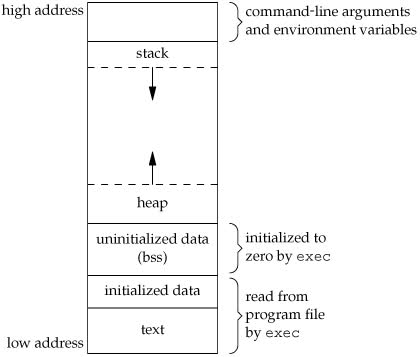
\includegraphics[width=.9\linewidth]{../../../files/program-image.jpg}
\caption{C程序的内存映像}
\end{figure}

这是一张典型的内存排列图,从高位到低位依次看,

\begin{enumerate}
\item 储存了命令行参数以及环境变量的区域/段;

\item Stack,在函数执行的时候,函数里所定义的变量(一般就是局部变量)以及相应的信息都会被储存到这里,当函数返回后这些变量以及信息就丢弃了.

并且每次调用函数时,该区域都会保存返回的地址以及调用者(caller)的环境信息.所以每次调用一个函数的时候都会在这个区域为函数的自动以及临时变量分配空间.

所以递归函数里面,每次调用一次就会使用一个栈帧,不同栈帧上的同名变量是不一样的.这个区域和叫做 \texttt{stack} 的数据结构一样有着同样的特性,而栈底位于高位,

内存从栈底开始增长.这个区域由编译器自动管理,与 \texttt{stack} 数据结构一样,栈帧是连续的,也就是说, \texttt{Stack} 上的内存分配是连续的.

(在某个函数的定义中,)在变量 \texttt{A} 之后定义的变量 \texttt{B} 必定是内存地址相邻的.

\item Heap,这个区域不像 \texttt{Stack} 一样有着同名数据结构的特性,动态内存分配就是发生在这个区域的,所谓动态分配就是分配的内存大小不定,甚至会在分配后发生改变,

所以这个区域上的内存分配不能够是连续的.比如 \texttt{char *s = malloc(s)},这个区域上面数据不会像 \texttt{Stack} 那样自动释放,

所以不在使用 \texttt{s} 的时候一定要手动释放: \texttt{free(s)}. Heap顶是位于高位的,与Stack相反,由于Heap底位于低位,所以Heap的内存是从低位往高位增长.

(\texttt{Stack} 也可以像 \texttt{Heap} 那样动态分配并且同时拥有 \texttt{Stack} 的自动管理特点, \texttt{alloca.h} 提供一个 \texttt{alloca} 的函数完成这样的事情).

\item 未初始数据 (Uninitialized Data Segment),又叫做 (bss, block started by symbol)区域/段,

包含了在函数外声明却未初始的变量,也就是未初始化的全局变量;

比如在函数外声明 \texttt{long sum[1000];}, \texttt{sum} 就是属于这个区域,

内核(kernel)会在程序执行前给这些数据给一个初始值, 0 或者 \texttt{null pointer}.

\item 已初始数据 (Initialized Data Segment)区域/段,包含了在函数外声明而且初始化了的变量,也就是已被初始化的变量;

比如在函数外声明 \texttt{int maxcount = 99}; \texttt{maxcount} 就是属于该区域;

\item Text 区域/段,包含了 \texttt{CPU} 能够执行的机器指令(machine instructions),也就是编译后的函数,

这块区域是可以共享的(sharable),所以这块才需要被加载进内存来方便频繁执行.

并且这块区域基本上是只读的,防止执行过程中被意外地修改.
\end{enumerate}


\\[0pt]


\texttt{a.out} 文件其它类型的区域有符号表(symbol table),调试信息(debugging information),动态共享库的连接表(linkage tables)等等,

但是只有上面6个区域才会被加载到内存中,所以这些额外区域不能算入内存映像中.

这里面的链接库值得一提,有两种类型的链接库,一种是静态的,还有一种动态的,动态的又叫共享库(shared libraries).

在编译时,编译器会把静态库链接到可执行文件上,这样可执行文件就会偏大,发布的时候只需要发布可执行文件.

而共享库则是在运行时被加载,发布程序的时候,共享库需要和可执行文件一起配套发布,可执行文件大小相对于使用静态时候小,

由于共享库不需要链接到可执行文件上,所以单独更新共享库只需要替换一下.

\begin{verbatim}
gcc -static source.c # 静态链接库
gcc source.c         # 使用共享库(默认)
\end{verbatim}


\subsection{EIEIO}
\label{sec:org06a2e32}

\section{Emacs 之深藏不漏}
\label{sec:org7340476}

\begin{verbatim}
写于 2019/12/12
\end{verbatim}

这部分专门记录本人对一些 Emacs 自带 mode 的学习记录,这些 mode 大部分都藏得很"深",

毕竟要一个一个试用需要很长时间,而且一些的学习成本很高,也并非每个人都有耐心学习,

但这些 mode 都能很方便的解决大部分问题,还是有学习的价值的,所以就专门有了这一个部分.

\subsection{Calc}
\label{sec:orgfc457b1}

\texttt{Calc} 是一个功能复杂而全面的 \texttt{mode},你可以用它来完成时区时间转换,绘图(需要gnuplot),各种代数运算(比如解决等式问题)等等各种数学任务.

就是因为 \texttt{Calc} 是太复杂了,时刻查阅文档是必须的,可能在过完官方的上手指南 \texttt{M-: (info "(Calc)Tutorial")} 时会觉得简单,

但实际上一用,或者说过一段时间再用的时候,都会有这种感觉: 做什么要用什么命令,要用哪个按键?

这就分情况了:

\textbf{如果知道要做什么计算的话}, 这文档就能解决这个问题了: \textbf{计算器命令索引} \texttt{M-: (info "(Calc)Command Index")}.

大部分情况都是知道做什么计算,但是不知道命令以及其对应的按键序列索引,

得益于 \texttt{Calc} 的开发者遵守 \textbf{语义一致} 以及 \textbf{定义的名字符合其含义} 的原则,

可以在 \textbf{计算器命令索引} 中通过 \texttt{\textbackslash{}C-s} 搜索关键字来查找出命令,再反查出命令对应的按键.

比如想要计算两个向量的叉积,那么通过 \texttt{\textbackslash{}C-s} 搜索叉积(\texttt{cross product})的英文中的关键字 \texttt{cross} 就可以找到 \texttt{calc-cross},

回车进去后可以看到它的描述是否符合要找的叉积(答案是肯定的),并且描述中还有命令对应按键.

\textbf{如果按键,想反查命令}, 那么这份文档可以很好的解决这个的问题: \texttt{(info "(Calc) Key Index")}.


\section{个人认为不错的的一些参考资源和博客}
\label{sec:org8e48402}

\begin{itemize}
\item 这篇文章给想进坑Emacs的人做思想工作

\url{https://github.com/redguardtoo/mastering-emacs-in-one-year-guide/blob/master/guide-en.org}

\item 挺不错的新手生存指南

\url{https://github.com/emacs-tw/emacs-101-beginner-survival-guide}

\item ElispCookbook,不过比PythonCookbook轻量,也就是不包括内置库的例子

\url{https://www.emacswiki.org/emacs/ElispCookbook}

\item EmacsWiki,虽然页面是比较乱,但是资源还是很赞的

\url{https://www.emacswiki.org/}

\item Xah Emacs,一个十分友好而全面的教程,作者是一个多年的Emacs用户,有很多不错的学习建议

\url{http://ergoemacs.org/index.html}

\item 一个挺有名的博客

\url{http://endlessparentheses.com/}

\item M-x Chris-An-Emacser,有不少有用的小技巧,比如摩斯密码

\url{https://chriszheng.science/}
\end{itemize}


\section{我与Emacs的一些事情}
\label{sec:org8b6fd27}

\begin{quote}
写于 2018/8/31
\end{quote}

\begin{itemize}
\item \textbf{最初}

我是在17年的4到6月中断断续续的接触Emacs,在这之前先是用VSCODE,本想长期使用VSCODE,一次意外改变了我的想法: \textbf{操作系统的桌面崩了}.

于是找了一个可以在CLI环境下面使用的编辑器,便有了一段很短的VIM经历,没记错的话就是4月份的时候,等到适应了VIM后就没想到过要用别的

编辑器了.然而一次偶然看到了一个贴提到了两个"神话"编辑器,其中一个就是VIM,另外一个就是Emacs.抱着好奇的想法去了解一下Emacs,不过

先入为主的想法让我并没有觉得Emacs有多好,特别是操作比起VIM的繁琐多了.由于当时手头上还有工作,所以Emacs就放一边了,继续利用VIM红

作.后面无聊的时候在一个周末里面找了各种关于Emacs配置Python开发环境的文章,配置好了用它来工作了,但还是不习惯,至于是什么时候习惯

的,那应该是我不再配置VIM的时候,当时已经把VIM负责的全部工作都交给Emacs处理了,整个过程花了一个月左右.其实VIM挺不错的,刚开始用

Emacs的时候我还用了 \texttt{Evil} 模拟VIM的按键,不过那个时候经常配置出错导致使用不了,而我又太依赖于VIM的按键导致了我一直没有熟悉Emacs

自带的按键,每次报错我都得使用别得编辑器修正配置.于是我下定决定不再依赖VIM了,正式进入人生中Emacs时代.

\item \textbf{现在}

现在开始学习如何写Package,其实之前也有尝试写过,写了几个"没用"的东西出来,现在看来就是在浪费时间,不过这让我自己明白了还有很多东西不懂和不足.

记录这些不足的目的是为了不断地提醒自己,不让自己偏离目标.

\begin{itemize}
\item 不足一: 学习态度不够端正,不够虚心.

总是认为在几天内熟练使用一门编程语言,在有其它语言基础的情况下,入门别语言的确是可以很快.

但是熟练使用就是另外一个个概念了:深入细节地学习语言的特性以及经过大量实践学习其中的细节.

还有就是不要老想着造轮子,造轮子并不具备创造性.而我也在这上面浪费了很多时间,抗拒使用别人的package,浪费大量时间花在所谓的"自己写"上面.

确实"自己写"的确可以学习到很多东西,但是效率太低了,而Emacs本身就是想给用户提供一个高效的工具,而不是让你去舍弃效率.可以选择在空余时间里深入学习.

在空余时间学习要注意做好知识管理,因为大部份人的空余时间都不会太多,因为学到的东西可能都很碎片,越是碎片就越容易忘掉,所以知识管理就很有必要了.

在这知识管理这点上我是做的不够好,导致很多知识忘了,以前付出时间和努力都白费了.还有不要忽视这一些碎片,时间久了回过头会发现收获很大.(因为我自己忘掉的

东西实在是太多了,我自己回过头来看都吓了一跳).

\item 不足二: 怕麻烦,行动力低下,总想一次做好

很多人都有这种心理: "这个很简单,做了只是浪费时间." 或者 "这个网上有解决方案,先休息一下稍后动手" 又或者 "这个工作量太大了,一两天做不完".

实践可能很简单,但是不真正操作一遍你是发现不了一些潜在的问题,比如系统环境的影响,一些软件依赖和版本问题.

还有尽早解决自己的拖延症,如果事情一点一点地拖下去,回过头你会发现明明是一件很简单地事情却拖了不少时间,更糟糕地是事情可能一直都不会完成甚至开始.拖延症/行动力低下是很多人在一件事情上面失败的主要原因.

至于工作量大的工作,要承认事实:"的确一两天是做不完的".别人的大地开源项目是怎么写出来的呢?通过 \texttt{commits} 可以发现别人也不是一两天做好的,他们也是一点点地写出来地.

如果事情/工作的确不能马上完成,那么请做好任务管理,记录要什么时候做什么,不这么做的话很有可能就回把这件事情给忘了.

\item 不足三: 害怕失败

曾经给 \texttt{fic-mode} 提交过两个 \texttt{pull request}, 第一个合并了,第二个被无视了.第二个是添加新功能的,第一次写地挺认真的,所以有点伤心,GitHub \texttt{issue} 和

\texttt{pull request} 产生了恐惧.现在想起来自己还是有点玻璃心,因为这是很平常的事情,很多人都有同样的经历,我只不过是其中一员.既然其他人能够挺过来,那么我也能.所以没必要

因为一次失败而气馁,现在觉得早点遇到失败也是好事.
\end{itemize}

\item \textbf{以后}

以后也会一直使用Emacs,因为这个开源项目已经改变我了:

\begin{enumerate}
\item 开始给别的项目提交 \texttt{pull request}

\item 跟别人交流

\item 能够静下心阅读代码和文档

\item 能够正视自己的缺点和不足

\item 开始虚心向别人学习
\end{enumerate}

有太多方面我想不起来,总的来说它对于我来说影响实在太大了,因此我也愿意把闲余时间投入到它的身上.

写这些的时候我才理解为什么有人说Emacs是一种生活态度了.
\end{itemize}
\end{document}
